
\errorcontextlines=200

\documentclass[finalspec]{sbmlpkgspec}
%% \documentclass[draftspec]{sbmlpkgspec}
\usepackage{microtype}
\usepackage{color}
\usepackage{todonotes}
\usepackage[color]{changebar}
\usepackage{xcolor}
\usepackage{soul}
\usepackage{subcaption}
\usepackage{longtable}

% Make changebars switchable to allow faster compilation:
%\def\fullchangebars{} % comment this out to simplify changebars and speed up compilation

% Macros just for this document:

\newcommand{\sbmlpkg}{\texorpdfstring{%
    \textls[-25]{\textsc{SBMLPkgSpec}}}{%
    \textsc{SBMLPkgSpec}}\xspace}
\newcommand{\sbmlpkghead}{\texorpdfstring{%
    \textls[-50]{\textsc{SBMLPkgSpec}}}{%
    \textsc{SBMLPkgSpec}}\xspace}
\newcommand{\sbmlpkgfile}{\literalFont{sbmlpkgspec.cls}\xspace}
\newcommand{\latex}{\LaTeX{}\xspace}
\newcommand{\tex}{\TeX{}\xspace}
\newcommand{\distURL}{http://sourceforge.net/projects/sbml/files/specifications/tex}
\newcommand{\srcURL}{https://sbml.svn.sourceforge.net/svnroot/sbml/trunk/project/tex/sbmlpkgspec}
\newcommand{\webURL}{http://sbml.org/Documents/Specifications/The_SBMLPkgSpec_LaTeX_class}
\newcommand{\cmd}[1]{\literalFont{\textbackslash #1}}

% Custom latex listing style, for use with the listings package.  The default
% highlights far too many things, IMHO.  This keeps it simple and only adjusts
% the appearance of comments within listings.

\lstdefinelanguage{mylatex}{%
  morekeywords={},%
  sensitive,%
  alsoother={0123456789$_},%$
  morecomment=[l]\%%
}[keywords,tex,comments]

\lstdefinestyle{latex}{language=mylatex}


%Command to format the listings containing SBOL RDF/XML serialization examples
\newcommand{\lstsetsbol}{
 \lstset{language=sbol,
        tabsize=2
 }
}

%Commands to format SBOL terms in the document

% Use sbolheading when you are referencing an SBOL data model class/field in a
% section heading.
\newcommand{\sbolheading}[1]{\texttt{#1}}

% Use sbol when you are referencing an SBOL data model class/field in text.
\newcommand{\sbol}[1]{\texttt{\hyperref[sec:#1]{#1}}}

% Use prov when you are using a class borrowed from Prov-O, this will prepend the "prov:" prefix as well
\newcommand{\prov}[1]{\texttt{\hyperref[sec:prov:#1]{prov:#1}}}

% Use provmult for Prov-O fields that appear in multiple classes, for example
% \sbolmult{hadRole:U}{hadRole}. This ensures the reference links to the correct
% section.
\newcommand{\provmult}[2]{\texttt{\hyperref[sec:prov:#1]{prov:#2}}}

% Use om when you are using a class borrowed from Ontology of Units & Measures, this will prepend the "om:" prefix as well
\newcommand{\om}[1]{\texttt{\hyperref[sec:om:#1]{om:#1}}}

% Use provmult for OM fields that appear in multiple classes, for example
% \sbolmult{hadUnit:M}{hadUnit}. This ensures the reference links to the correct
% section.
\newcommand{\ommult}[2]{\texttt{\hyperref[sec:om:#1]{om:#2}}}

% Use sbolmult for SBOL fields that appear in multiple classes, for example
% \sbolmult{types:CD}{types}. This ensures the reference links to the correct
% section.
\newcommand{\sbolmult}[2]{\texttt{\hyperref[sec:#1]{#2}}}

% Rarely used. Use refObj you want to put the field in angle brackets.
\newcommand{\refObj}[1]{$\langle$#1$\rangle$}

%Command to format external terms in the document
\newcommand{\external}[1]{\texttt{#1}}

%Commands to highlight SBOL versions
%\newcommand{\threeonezero}[1]{%
%	\cbcolor{red}
%	\cbstart%
%	{\color{red}%
%		\version{3.1.0}%
%		#1
%	}
%	\cbend
%}

% -----------------------------------------------------------------------------
% Start of document
% -----------------------------------------------------------------------------

\begin{document}

\packageTitle{\latex Class for SBML Package Specifications}		
\packageVersion{Version 3.0.1}		
\packageVersionDate{October 15, 2020}
 
\title{
  Synthetic Biology Open Language \texorpdfstring{\\[3pt]}{}\mbox{(SBOL) Version~3.0.1}}

\author{{\bf Editors:}\hfil\\
\begin{tabular}{l>{\hspace*{15pt}}r}
Hasan Baig & \emph{University of Connecticut, USA}\\   
Pedro Fontanarrosa & \emph{University of Utah, USA}\\   
Vishwesh Kulkarni & \emph{University of Warwick, UK}\\ 
James McLaughlin & \emph{Newcastle University, UK}\\
Prashant Vaidyanathan & \emph{Microsoft Research, UK}\\ 
\multicolumn{2}{c}{\href{mailto:editors@sbolstandard.org}{\sffamily editors@sbolstandard.org}}\\
\\
\multicolumn{2}{c}{ {\bf Chair:} } \\
Chris Myers		& \emph{University of Utah, USA}\\
\\
\multicolumn{2}{c}{{\bf Additional authors:}} \\
Bryan Bartley & \emph{Raytheon BBN Technologies, USA} \\
Jacob Beal & \emph{Raytheon BBN Technologies, USA}\\ 
Matthew Crowther & \emph{Newcastle University, UK} \\
Thomas Gorochowski & \emph{University of Bristol, UK}\\
Raik Gr\"unberg & \emph{KAUST, SA}\\
Goksel Misirli & \emph{Keele University, UK}\\ 
Thomas Mitchell & \emph{Raytheon BBN Technologies, USA} \\
Ernst Oberortner & \emph{DOE Joint Genome Institute, USA}\\
James Scott-Brown & \emph{University of Oxford, UK} \\
Anil Wipat & \emph{Newcastle University, UK}\\
\end{tabular}\\
}

\maketitlepage

\maketableofcontents

% -----------------------------------------------------------------------------
\section{Purpose}
% -----------------------------------------------------------------------------

Synthetic biology builds upon genetics, molecular biology, and metabolic engineering by applying engineering principles to the design of biological systems.
When designing a synthetic system, synthetic biologists need to exchange information about multiple types of molecules, the intended behavior of the system, and actual experimental measurements.
Furthermore, there are often multiple aspects to a design such as a specified nucleic acid sequence (e.g., a sequence that encodes an enzyme or transcription factor), the molecular interactions that a designer intends to result from the introduction of this sequence (e.g., chemical modification of metabolites or regulation of gene expression), and the experiments and data associated with the system. All these perspectives need to be connected together to facilitate the engineering of biological systems.

The \emph{Synthetic Biology Open Language} (SBOL) has been developed as a standard to support the specification and exchange of biological design information in synthetic biology,
following an open community process involving both ``wet'' bench scientists and ``dry'' scientific modelers and software developers, across academia, industry, and other institutions.
Previous nucleic acid sequence description formats lack key capabilities relative to SBOL, as shown in \ref{f:sequence}.
Simple sequence encoding formats such as FASTA encode little besides sequence information.
More sophisticated formats such as GenBank and Swiss-Prot provide a flat annotation of sequence features that is well suited to describing natural systems but unable to represent the functional relations and multi-layered design structure common to engineered systems.
Modeling languages, such as the Systems Biology Markup Language (SBML) ~\cite{SBML}, can be used represent biological processes, but are not sufficient to represent the associated nucleotide or amino acid sequences.
SBOL covers both of these needs, by providing a modular and hierarchical representation of the structure and function of a genetic design, as well as its relationship to and use within experiment plans, data, models, etc.

\begin{figure}[htbp!]
\centering
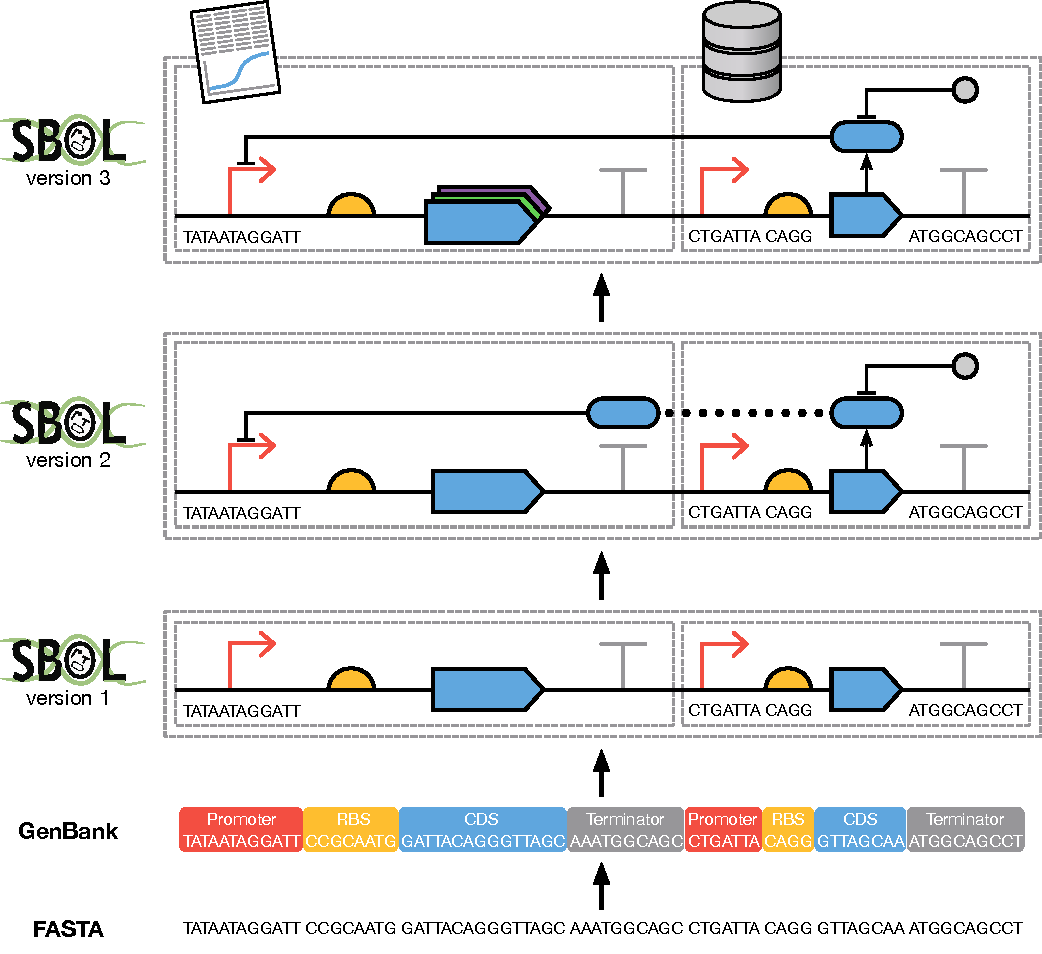
\includegraphics[width=0.8\textwidth]{images/SBOL3-evolution.pdf}
\caption{SBOL extends prior sequence description formats to represent both the structure and function of a genetic design in a modular, hierarchical manner, as well as its relationship to, and use within, experiments, plans, data, models, etc.}
\label{f:sequence}
\end{figure}

SBOL uses existing Semantic Web practices and resources, such as \emph{Uniform Resource Identifiers} (\sbol{IRI}s) and ontologies, to unambiguously identify and define biological system elements,
and to provide serialization formats for encoding this information in electronic data files.
The SBOL standard further describes the rules and best practices on how to use this data model and populate it with relevant design details.
The definition of the data model, the rules on the addition of data within the format, and the representation of this in electronic data files are intended to make the SBOL standard a useful means of promoting data exchange between laboratories and between software programs.

\subsection*{Differences from Prior Versions of SBOL}

SBOL 1 focused on representing the structural aspects of genetic designs: it allowed the exchange of information about DNA designs and their sequence features, but could not represent molecules other than DNA or the functional aspects of designs. SBOL 2 enabled the description and exchange of hierarchical, modular representations of both the intended structure and function of designed biological systems, as well as providing support for representing provenance, combinatorial designs, genetic design implementations, external file attachments, experimental data, and numerical measurements.
SBOL 3.0, defined by this document, condenses and simplifies these prior representations based on experiences in deployment across a variety of scientific and industrial settings.

Specifically, SBOL 3.0 improves on its predecessor SBOL 2.3 by:
\begin{itemize}
\item Separating sequence features from part/sub-part relationships.
\item Renaming ComponentDefinition/Component to Component/SubComponent.
\item Merging Component and Module classes.
\item Ensuring consistency between data model and ontology terms.
\item Extending the means to define and reference SubComponents.
\item Refining requirements on object IRIs.
\item Enabling graph-based serialization.
\item Moving to Systems Biology Ontology (SBO) for Component types.
\item Making all sequence associations explicit.
\item Making interfaces explicit.
\item Generalizing SequenceConstraints into a general structural Constraint class.
\item Expanding the set of allowed sequence constraints.
\end{itemize}



% -----------------------------------------------------------------------------
\section{A Brief History of SBOL}
% -----------------------------------------------------------------------------
%Add yourself if you have helped and aren't on the list

The SBOL effort was started in 2006 with the goal of developing a data exchange standard for genetic designs. Herbert Sauro (University of Washington) secured a grant from Microsoft in the field of computational synthetic biology, which was used to fund the initial meeting in Seattle on April 26-27, 2008. This workshop was organized by Herbert Sauro, Sean Sleight, and Deepak Chandran, and included talks by Raik Gruenberg, Kim de Mora, John Cumbers,  Christopher Anderson, Mac Cowell, Jason Morrison, Jean Peccoud, Ralph Santos, Andrew Milar, Vincent Rouilly, Mike Hucka, Michael Blinov, Lucian Smith, Sarah Richardson, Guillermo Rodrigo, Jonathan Goler, and Michal Galdzicki. 

% Go over past meetings and mention who funded them, eg Douglas Densmore.

Michal's early efforts were instrumental in making SBOL successful. As part of his doctoral work, he led the development of PoBol (Provisional BioBrick Language), as SBOL was originally known. He organized annual workshops from 2008 to 2011 and kept the idea of developing a genetic design standard alive. The original SBOL 1.0 was developed by a small group of dedicated researchers calling themselves the Synthetic Biology Data Exchange Working Group, meeting at Stanford in 2009 and Anaheim, CA in 2010.  During the Anaheim meeting, the community decided to write a letter to Nature Biotechnology highlighting the issue of reproducibility in synthetic biology~\cite{Peccoud2011}. This letter was initiated by Jean Peccoud and submitted by participants of the Anaheim meeting, including Deepak Chandran, Douglas Densmore, Dmytriv, Michal Galdzicki, Timothy Ham, Cesar Rodriquez, Jean Peccoud, Herbert Sauro, and Guy-Bart Stan. The overall pace of development quickened when several new members joined at the next workshop in Blacksburg, Virginia on January 7-10, 2011. This early work was also supported by an STTR grant from the National Institute of Health (NIH \#1R41LM010745 and \#9R42HG006737, from 2010-13) in collaboration with Clark \& Parsia, LLC (Co-PIs: John Gennari and Evren Sirin). New members included Cesar Rodriguez, Mandy Wilson, Guy-Bart Stan, Chris Myers, and Nicholas Roehner.

The SBOL Developers Group was officially established at a meeting in San Diego in June 2011.  Rules of governance were established, and the first SBOL editors were elected: Mike Galdzicki, Cesar Rodriguez, and Mandy Wilson. At our next meeting in Seattle in January 2012, Herbert Sauro was elected the SBOL chair, and two new editors were added: Matthew Pocock and Ernst Oberortner.  New developers joining at these workshops included several representatives from industry, Kevin Clancy, Jacob Beal, Aaron Adler, and Fusun Yaman Sirin. New members from Newcastle University included Anil Wipat, Matthew Pocock, and Goksel Misirli.

Development of the first software library (libSBOLj) based on the SBOL standard was initiated by Allan Kuchinsky, a research scientist from Agilent, at the 2011 meeting.  By the time of the 2012 meeting, the first data exchange between software tools using SBOL was conducted when a design was passed from Newcastle University's VirtualParts Repository to Boston University's Eugene tool, and finally to University of Utah's iBioSim tool. 

SBOL 1.0 was officially released in October 2011.  In March 2012, SBOL 1.1 was released, the version that this document replaces. SBOL 1.1 did not make any major changes, but provided a number of small adjustments and clarifications, particularly around the annotation of sequences.  Multi-institutional data exchange using SBOL 1.1 was later demonstrated in Nature Biotechnology \cite{galdzicki2014synthetic}. 

While SBOL 1.1 had a number of significant advantages over the GenBank representation of DNA sequences, such as representing hierarchical organization of DNA components, it was still limited in other respects. The major topic of discussion at the 8th SBOL Workshop at Boston University in November 2012 was how to address these shortcomings through extensions.  Several extensions were discussed at this meeting, such as a means to describe genetic regulation, which later became important classes in the current 2.x specification.  

A general framework for SBOL 2.0 emerged at the 9th SBOL workshop at Newcastle University in April 2013.  Subsequently, Nicholas Roehner, Matthew Pocock, and Ernst Oberortner drafted a proposal for SBOL 2.0, and Nicholas presented this proposal at the SEED conference in Los Angeles in July 2014 \cite{roehner2014proposed}.  The proposed 2.0 data model was discussed over the course of the 10th, 11th, and 12th workshops.  
The SBOL 2.0 specification document was drafted at the 13th workshop in Wittenberg, Germany. The SBOL 2.x data model presented was essentially the result of these meetings and ongoing discussions conducted through the SBOL Developers mailing lists, plus minor adjustments and updates approved by the community through subsequence meetings and mailing list discussions.

From 2014 to 2019, development of SBOL 2.x was funded in large part by a grant from the National Science Foundation (DBI-1355909 and DBI-1356041).  The SBOL 2.x specification documents and the supporting software libraries are due in no small part to this support. Any opinions, findings, and conclusions or recommendations expressed in SBOL materials are those of the author(s) and do not necessarily reflect the views of the National Science Foundation.

The Computational Modeling in Biology Network (\href{http://www.co.mbine.org}{COMBINE}) holds regular workshops at which synthetic biologists and systems biologists work toward a common goal of integrating biological knowledge through interoperable and non-overlapping data standards. Several SBOL Developers proposed that SBOL join this larger standards community after attended a COMBINE workshop in April 2014.  The proposal passed and SBOL workshops have been co-located with COMBINE meetings since the 11th workshop at the University of Southern California in August 2014.

In 2019 the SBOL Industrial Consortium was established as a pre-competitive non-profit organization supporting innovation, dissemination, and integration of SBOL standards, tools and practices for practical applications in an industrial environment. The SBOL Industrial Consortium meets regularly to coordinate its activities, and organises an Industrial Advisory Board to give an industrial perspective on SBOL, as well as providing financial support for projects, activities, and infrastructure within the SBOL community.
Member organsiations include Raytheon BBN Technologies, Doulix, Integrated DNA Technologies, Twist Bioscience, Amyris, Inscripta, Teselagen, Shipyard Toolchains, and Zymergen.

Discussions related to SBOL 3 began at the COMBINE meetings and on the mailing list beginning in the summer of 2018.  Over the next year and a half, several SBOL Enhancement Proposals (SEPs) were written and discussed.  During the early months of 2020, these SEPs were voted on and approved by the SBOL community.  The initial version of the SBOL 3 specification was drafted during HARMONY 2020 at the European Bioinformatics Institute (EBI) in Hinxton, United Kingdom in March 2020.

The authors would also like to thank Michael Hucka for developing the LaTeX style file used to develop this document~\citep{hucka2017sbmlpkgspec}.



% % -----------------------------------------------------------------------------
\section{Overview of SBOL}
% % -----------------------------------------------------------------------------

Synthetic biology designs can be described using:
\begin{itemize}
\item Structural terms, e.g., a set of annotated sequences or information about the chemical makeup of components.
\item Functional terms, e.g., the way that components might interact with each other. 
\end{itemize}

As an example, consider an expression cassette, such as the one found in the plasmid pUC18~\cite{L08752.1}.
The system is designed to visually indicate whether a gene has been inserted into the plasmid: 
in the presence of IPTG, it expresses an enzyme that hydrolyses X-gal to form a blue product, but successful insertion disrupts the expression cassette and prevents the formation of this product. 
Internally, it has a number of parts, including a promoter, the lac repressor binding site, and the lacZ coding sequence.
These parts have specific component-level interactions with IPTG and X-gal, as well as native host gene products, transcriptional machinery, and translational machinery that collectively cause the desired system-level behavior.

In SBOL 3, both the structural and functional aspects are described using a class called \sbol{Component}, as depicted in \ref{images:overview1}.  
Namely, to represent structural aspects, a \sbol{Component} can include \sbol{Feature}s, some of which may be at some \sbol{Location} within a \sbol{Sequence}.  
A \sbol{Component} can also include \sbol{Constraint}s between these features.  
To represent functional aspects, a \sbol{Component} can include \sbol{Interaction}s that can refer to relationships between participating \sbol{Feature}s.  
Finally, a \sbol{Component} can have its behavior described using a \sbol{Model}.

\begin{figure}[ht]
\begin{center}
  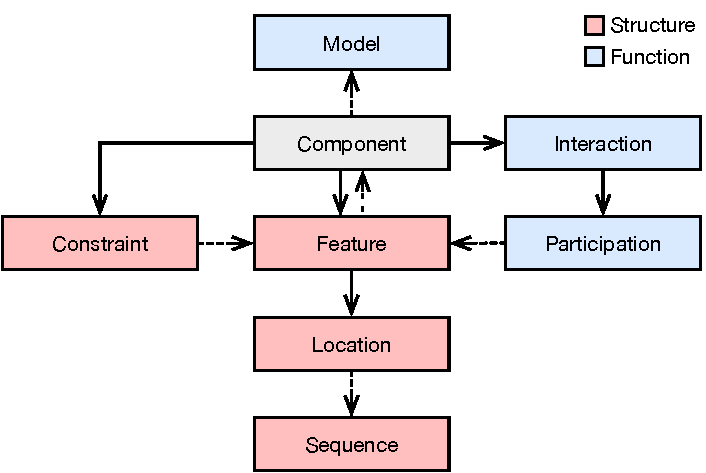
\includegraphics[scale=0.85]{images/SBOL3-main-classes.pdf}
\caption{The SBOL \sbol{Component} object and related objects.  
	Solid arrows indicates ownership, whereas a dashed arrow represents a reference to an object of another class.  
	Red boxes represent structural objects, while blue boxes represent functional objects.  
	To represent structural aspects, a \sbol{Component} can include \sbol{Feature}s, which may refer to \sbol{Location}s within a \sbol{Sequence}. 
	A \sbol{Component} can also include \sbol{Constraint}s between these features.  
	To represent functional aspects, a \sbol{Component} can include \sbol{Interaction}s that can refer to relationships between participating \sbol{Feature}s.  
	Finally, a \sbol{Component} can have its behavior described using a \sbol{Model}.}
\label{images:overview1}
\end{center}
\end{figure}

To continue with the pUC18 example, the description would begin with a top-level \sbol{Component} that represents the entire system.  
This \sbol{Component} specifies the structural elements that make up the cassette by referencing a number of \sbol{SubComponent} objects. These would include the DNA \sbol{SubComponent} for the promoter and the simple chemical
\sbol{SubComponent} for IPTG, for example.  
The \sbol{Component} objects can be organized hierarchically.  
For example, the plasmid \sbol{Component} might reference \sbol{SubComponent}s for the promoter, coding sequence, etc.  
Each \sbol{Component} object can also include the actual \sbol{Sequence} information (if available), as well as \sbol{SubComponent} objects that identify the \sbol{Location}s of the promoters, coding sequences, etc., on the \sbol{Sequence}.  
In order to specify functional information, the \sbol{Component} can also specify \sbol{Interaction} objects that describe any qualitative relationships among \sbol{SubComponent} \sbol{Participation}s, such as how IPTG and X-gal interact with the gene products.  Finally, a \sbol{Component} object can point to a \sbol{Model} object that provides a reference to a complete computational model expressed in a language such as SBML~\cite{SBML}, CellML~\cite{CellML}, or MATLAB~\cite{matlab}.

Whereas \ref{images:overview1} provides an overview of the classes used for describing designs within the SBOL 3 data model,  \ref{images:overview2} shows the rest of the classes used to describe the usage of a design within design-build-test-learn workflows in general.
In particular, designs can be expressed using \sbol{CombinatorialDerivation}s, \sbol{Component}s, and \sbol{Sequence}s.
These can describe not only genetic designs, but also designs for strains, multicellular systems, media, samples, etc.
A \sbol{CombinatorialDerivation} allows one to specify a design pattern where individual \sbol{SubComponent}s can be selected from a set of variants.  
The \sbol{Implementation} class is the build class, and it is used to represent physical artifacts like an actual sample of a plasmid.  
The \sbol{Experiment} and \sbol{ExperimentalData} classes are the test classes, allowing description of a collection of data generated in an experiment.  
The \sbol{Model} class, discussed earlier, associates learned information with a design.
The \prov{Activity} class is taken from the provenance ontology (PROV-O), which is described in~\ref{sec:provenance}.  For example, a build \prov{Activity} describes how an \sbol{Implementation} is constructed using a \sbol{Component} description.  On the other hand, a test \prov{Activity} describes how an \sbol{Experiment} is conducted using an \sbol{Implementation} artifact.  The \sbol{Collection} class has members, which can be of any of these types or \sbol{Collection}s themselves.  
Finally, all of these objects can refer to objects of the \sbol{Attachment} class, which are used to link out to external data (images, spreadsheets, textual documents, etc.). 
The next sections provide complete definitions and details for all of these classes.

\begin{figure}[ht]
\begin{center}
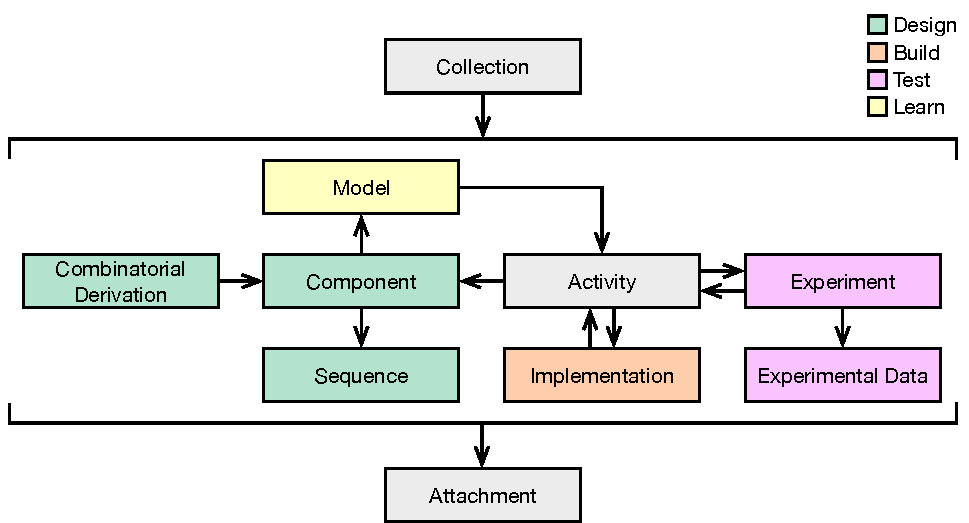
\includegraphics[scale=0.85]{images/SBOL3-top-levels.pdf}
\caption{Main classes of information represented by the SBOL 3 standard, and their relationships.  Green boxes represent design classes, orange boxes represent build classes, purple boxes represent test classes, yellow boxes represent learn classes, and the gray boxes represent additional utility classes.  Each of these classes will be described in more detail below.}
\label{images:overview2}
\end{center}
\end{figure}


% -----------------------------------------------------------------------------
\section{Conventions}
% -----------------------------------------------------------------------------

This section provides some preliminary information to aid in the understanding of the specification.
The SBOL data model is specified using Unified Modeling Language (UML) 2.0 diagrams \href{http://www.omg.org/spec/UML/2.0/}{(OMG 2005)}. This section reviews terminology conventions, the basics of UML diagrams, and our naming conventions.

\subsection{Terminology Conventions}

This document indicates requirement levels using the controlled vocabulary specified in \href{https://tools.ietf.org/html/rfc2119}{IETF RFC 2119}.
In particular, the key words ``MUST'', ``MUST NOT'', ``REQUIRED'', ``SHALL'', ``SHALL NOT'', ``SHOULD'', ``SHOULD NOT'', ``RECOMMENDED'', ``MAY'', and ``OPTIONAL'' in this document are to be interpreted as described in RFC 2119.

\begin{itemize}
\item The words ``MUST'', ``REQUIRED'', or ``SHALL'' mean that the item is an absolute requirement.
\item The phrases ``MUST NOT'' or ``SHALL NOT'' mean that the item is an absolute prohibition.
\item The word ``SHOULD'' or the adjective ``RECOMMENDED'' mean that there might exist valid reasons in particular circumstances to ignore a particular item, but the full implications need to be understood and carefully weighed before choosing a different course.
\item The phrases ``SHOULD NOT'' or ``NOT RECOMMENDED'' mean that there might exist valid reasons in particular circumstances when the particular behavior is acceptable or even useful, but the full implications need to be understood and the case carefully weighed before implementing any behavior described with this label.
\item The word ``MAY'' or the adjective ``OPTIONAL'' mean that an item is truly optional.
\end{itemize}

\subsection{UML Diagram Conventions}
\label{sec:umldiagrams}

The types of biological design data modeled by SBOL are commonly referred to as {\em classes}, especially when discussing the details of software implementation. Each SBOL class can be instantiated by many SBOL objects. These objects MAY contain data that differ in content, but they MUST agree on the type and form of their data as dictated by their common class. Classes are represented in UML diagrams as rectangles labeled at the top with class names (see \ref{fig:uml_sampler} for examples).

\begin{figure}[ht]
\begin{center}
  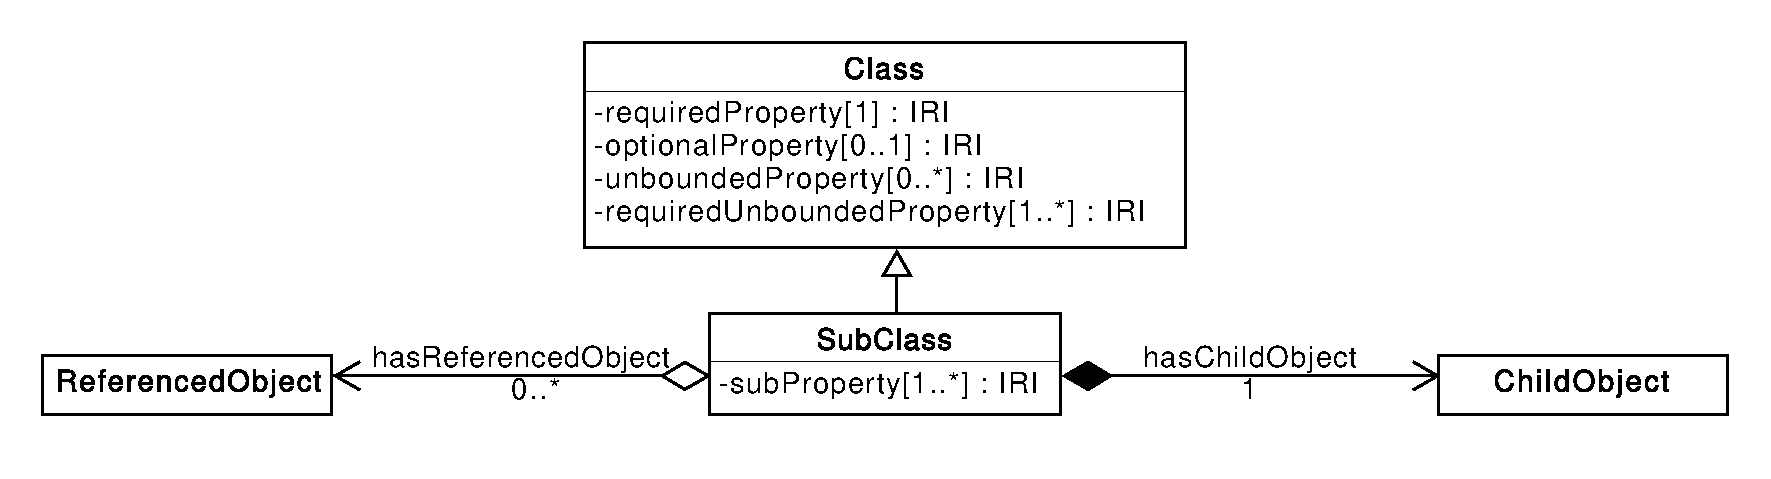
\includegraphics[width=\textwidth]{uml/uml_sampler.pdf}
\caption{Examples of UML diagram conventions used in this document}
\label{fig:uml_sampler}
\end{center}
\end{figure}

Classes can be connected to other classes by association properties, which are represented in UML diagrams as arrows. These arrows are labeled with data cardinalities in order to indicate how many values a given association property can possess (see below). The remaining (non-association) properties of a class are listed below its name. Each of the latter properties is labeled with its data type and cardinality.

In the case of an association property, the class from which the arrow originates is the owner of the association property. A diamond at the origin of the arrow indicates the type of association.
Open-faced diamonds indicate shared aggregation, also known as a reference, in which the owner of the association property exists independently of its value.

By contrast, filled diamonds indicate composite aggregation, also known as a part-whole relationship, in which the value of the association property MUST NOT exist independently of its owner.
In addition, in the SBOL data model, it is REQUIRED that the value of each composite aggregation property is a unique SBOL object (that is, not the value for more than one such property).
Note that in all cases, composite aggregation is used in such a way that there SHOULD NOT be duplication of such objects.
Such objects are also commonly referred to as ``child'' objects, and their owning objects as ``parent'' objects.

All SBOL properties are labeled with one of several restrictions on data cardinality. These are:

\begin{itemize}

\item $1$ - REQUIRED, one: there MUST be exactly one value for this property.

\item $0 \ldots 1$ - OPTIONAL: there MAY be a single value for this property, or it MAY be absent.

\item $0 \ldots *$ - unbounded: there MAY be any number of values for this property, including none.

\item $1 \ldots *$ - REQUIRED, unbounded: there MAY be any number of values for this property, as long as there is at least one.

\item $n \ldots *$ - at least: there MUST be at least $n$ values for this property.

\end{itemize}

Finally, classes can inherit the properties of other classes. Inheritance relationships are represented in UML diagrams as open-faced, triangular arrows that point from the inheriting class to the inherited class. Some classes in the SBOL data model cannot be instantiated as objects and exist only to group common properties for inheritance. These classes have italicized names and are known as abstract classes.

\subsection{Naming and Typographic Conventions}
\label{sec:nameconventions}

SBOL classes are named using upper ``camel case,'' meaning that each word is capitalized and all words are run together without spaces, e.g., \sbol{Identified}, \sbol{SequenceFeature}.
Properties, on the other hand, are named using lower camel case, meaning that they begin lowercase (e.g., \sbolmult{role:C}{role}) but if they consist of multiple words, all words after the first begin with an uppercase letter (e.g., \sbol{roleIntegration}).

SBOL properties are always given singular names irrespective of their cardinality, e.g., \sbolmult{role:C}{role} is used rather than \sbolmult{role:C}{role} even though a component can have multiple roles.
This is because each relation can potentially stand on its own, irrespective of the existence of others in the set.

\threezeroone{Two conventions are used for property names, {\tt name} and {\tt hasName}.  
When a property is pointing to a class using the same name, it uses the {\tt hasName} convention (e.g., the \sbol{Component} class uses \sbol{hasFeature} to point to a \sbol{Feature} object).
When the property uses a different name than the class of the object it points to, it uses the {\tt name} convention instead (e.g., the \sbol{Constraint} class uses \sbol{subject} to point to a \sbol{Feature} object).}


% -----------------------------------------------------------------------------
\section{Identifiers and Primitive Types}
% -----------------------------------------------------------------------------

\subsection{Uniform Resource Identifiers}
\label{sec:URIstructure}

As SBOL is built upon the Resource Description Framework (RDF), all class instances are identified by a Uniform Resource Identifier (URI).  In the SBOL data model, the value of an association property MUST be a \sbol{URI} or set of \sbol{URI}s that refer to SBOL objects belonging to the class at the tip of the arrow.  Every \sbol{Identified} object's URI MUST be globally unique among all other \sbol{Identified} object URIs. It is also highly RECOMMENDED that the \sbol{URI} structure follows the recommended best practices for compliant \sbol{URI}s specified in \ref{sec:compliant}.

Whenever a \sbol{TopLevel} object's URI is a URL (e.g., following the conventions of HTTP(S) rather than a UUID), its structure MUST comply with the following rules:

\begin{itemize}

 \item A \sbol{TopLevel} URL MUST use the following pattern:
  \texttt{[namespace]/[local]/[displayId]},  where \texttt{namespace} and \sbol{displayId} are required fragments, and the \texttt{local} fragment is an optional relative path.
  
  	For example, a \sbol{Component} might have the URL~\path{https://synbiohub.org/public/igem/BBa_J23070}, where \texttt{namespace} is \path{https://synbiohub.org}, \texttt{local} is \path{public/igem}, and \texttt{displayId} is \path{BBa_J23070}.

  \item A \sbol{TopLevel} object's URL MUST NOT be included as prefix for any other \sbol{TopLevel} object.
  
  	For example, the \path{BBa_J23070_seq} \sbol{Sequence} object cannot have a URL of \path{https://synbiohub.org/public/igem/BBa_J23070/BBa_J23070_seq}, since the \path{https://synbiohub.org/public/igem/BBa_J23070} prefix is already used as a URL for the \path{BBa_J23070} \sbol{Component} object.

  \item The URL of any child or nested object MUST use the following pattern:\texttt{[parent]/[displayId]}, where \texttt{parent} is the URL of its parent object.
	Multiple layers of child objects are allowed using the same\\ \texttt{[parent]/[displayId]} pattern recursively.
	
	For example, a \sbol{SequenceFeature} object owned by the \path{BBa_J23070} \sbol{Component} and having a \sbol{displayId} of \threezeroone{\st{annotation1}} \texttt{SequenceFeature1} will have a URL of \path{https://synbiohub.org/public/igem/BBa_J23070/SequenceFeature1}.
	Similarly, \threezeroone{\st{the loc1 Location child of the annotation1 SequenceFeature object will have the URL}} \threezeroone{if the \texttt{SequenceFeature1} object has a \sbol{Location} child object with a \sbol{displayId} of \texttt{Location1}, then that object will have the URL\\ \path{https://synbiohub.org/public/igem/BBa_J23070/SequenceFeature1/Location1}.}
  \end{itemize}

\threezeroone{\subsection{SBOL URIs}

The SBOL namespace, which is \url{http://sbols.org/v3\#}, is used to indicate which entities and properties in an SBOL document are defined by SBOL. 
For example, the URI of the type \sbol{Component} is \url{http://sbols.org/v3\#Component}. 
This convention is assumed throughout the specification.
The SBOL namespace MUST NOT be used for any entities or properties not defined in this specification.  

Other namespaces are also used by SBOL, however.
Where possible, we have re-used predicates from widely-used terminologies (such as Dublin Core~\cite{dcmi2012}) to expose as much of the data as practical to such standard RDF tooling.
Similarly, existing biological ontologies are used where applicable for specifying types, roles, etc.
Likewise, Section~\ref{sec:complementaryStandards} details complementary standards that are RECOMMENDED for use in combination with SBOL.}


\subsection{Primitive Data Types}
\label{sec:datatypes}
\label{sec:String}
\label{sec:Integer}
\label{sec:Long}
\label{sec:Double}
\label{sec:Boolean}
\label{sec:URI}
\label{sec:literal}

When SBOL uses simple ``primitive'' data types such as \sbol{String}s or \sbol{Integer}s, these are defined as the following specific formal types:
\threezeroone{
  \begin{itemize}
\item \sbol{String}: \href{http://www.w3.org/2001/XMLSchema}{http://www.w3.org/2001/XMLSchema\#string}\\
  {\em Example: ``LacI coding sequence''}
\item \sbol{Integer}: \href{http://www.w3.org/2001/XMLSchema}{http://www.w3.org/2001/XMLSchema\#integer}\\
  {\em Example: 3}
\item \sbol{Long}: \href{http://www.w3.org/2001/XMLSchema}{http://www.w3.org/2001/XMLSchema\#long}\\
  {\em Example: 9223372036854775806}
\item \sbol{Double}: \href{http://www.w3.org/2001/XMLSchema}{http://www.w3.org/2001/XMLSchema\#double}\\
  {\em Example: 3.14159}
\item \sbol{Boolean}: \href{http://www.w3.org/2001/XMLSchema}{http://www.w3.org/2001/XMLSchema\#boolean}\\
  {\em Example: \external{true}}
\end{itemize}
}
The term \sbol{literal} is used to denote an object that can be any of the five types listed above.

In addition to the simple types listed above, SBOL also uses objects with types \emph{Uniform Resource Identifier} (\sbol{URI}). It is important to realize that in RDF, a \sbol{URI} might or might not be a resolvable URL (web address).  A \sbol{URI} is always a globally unique identifier within a structured namespace.  In some cases, that name is also a reference to (or within) a document, and in some cases that document can also be retrieved (e.g., using a web browser).



\section{SBOL Data Model}\label{sec:model}

The section describes the SBOL data model in detail.  Best practices when using the standard can be found in \ref{sec:bestpractices}.

\subsection{Identified}
\label{sec:Identified}

All SBOL-defined classes are directly or indirectly derived from the \sbol{Identified}  abstract class.
This inheritance means that all SBOL objects are uniquely identified using \sbol{URI}s that uniquely refer to these objects within an SBOL document or at locations on the World Wide Web.

As shown in \ref{uml:identified}, the \sbol{Identified} class includes the following properties: \sbol{displayId},  \sbol{name}, \sbol{description}, \prov{wasDerivedFrom}, and \prov{wasGeneratedBy}. 

\begin{figure}[ht]
\begin{center}
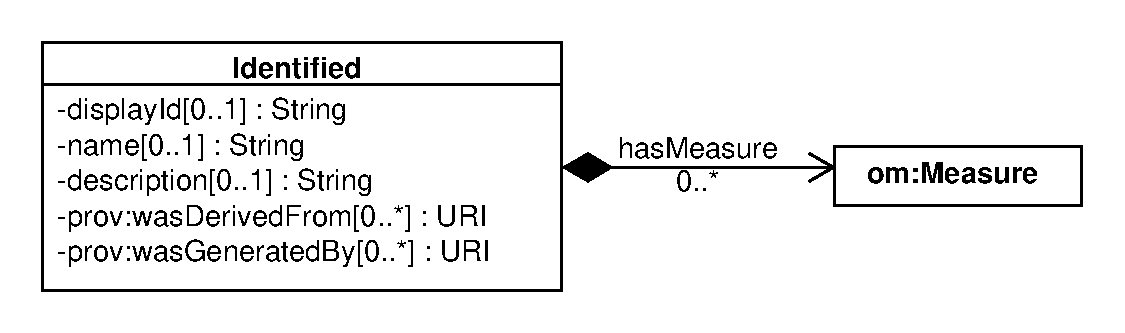
\includegraphics[scale=0.6]{uml/identified}
\caption[]{Diagram of the \sbol{Identified} abstract class and its associated properties}
\label{uml:identified}
\end{center}
\end{figure}
  
\subparagraph{The \sbolheading{displayId} property}
\label{sec:displayId}
The \sbol{displayId} property is an OPTIONAL identifier with a data type of \sbol{String}. This property is intended to be an intermediate between a URI and the \sbol{name} property that is machine-readable, but more human-readable than the full URI of an object.

If the \sbol{displayId} property is used, then its \sbol{String} value MUST be composed of only alphanumeric or underscore characters and MUST NOT begin with a digit.

Note that for objects whose URI is a URL, the requirements on URL structure in \ref{sec:URIstructure} imply that the \sbol{displayId} MUST be set.

\subparagraph{The \sbolheading{name} property}
\label{sec:name}

The \sbol{name} property is OPTIONAL and has a data type of \sbol{String}. This property is intended to be displayed to a human when visualizing an \sbol{Identified} object.

If an \sbol{Identified} object lacks a name, then software tools SHOULD instead display the object's \sbol{displayId} or URI.
It is RECOMMENDED that software tools give users the ability to switch perspectives between \sbol{name} properties that are human-readable and \sbol{displayId} properties that are less human-readable, but are more likely to be unique.

\subparagraph{The \sbolheading{description} property}
\label{sec:description}

The \sbol{description} property is OPTIONAL and has a data type of \sbol{String}. This property is intended to contain a more thorough text description of an \sbol{Identified} object.

\subparagraph{The \sbolheading{prov:wasDerivedFrom} property}
\label{sec:prov:wasDerivedFrom}
An \sbol{Identified} object MAY have zero or more \prov{wasDerivedFrom} properties, each of type URI. This property is defined by the PROV-O ontology and is located in the \url{https://www.w3.org/ns/prov#} namespace (Reference: \ref{sec:provenance}).

An \sbol{Identified} object with this property refers to one or more non-SBOL resources or SBOL \sbol{Identified} objects from which this object was derived. 
 An \sbol{Identified} object MUST NOT refer to itself via its own \prov{wasDerivedFrom} property or form a cyclical chain of references via its \prov{wasDerivedFrom} property and those of other \sbol{Identified} objects. For example, the reference chain ``$A$ was derived from $B$ and $B$ was derived from $A$'' is cyclical.

\subparagraph{The \sbolheading{prov:wasGeneratedBy} property}
\label{sec:prov:wasGeneratedBy}
An \sbol{Identified} object MAY have zero or more \prov{wasGeneratedBy} properties, each of type URI. This property is defined by the PROV-O ontology and is located in the \url{https://www.w3.org/ns/prov#} namespace (Reference: \ref{sec:provenance}).

An \sbol{Identified} object with this property refers to one or more \prov{Activity} objects that describe how this object was generated.
Provenance history formed by \prov{wasGeneratedBy} properties of \sbol{Identified} objects and entity references in \prov{Usage} objects MUST NOT form circular reference chains.

\subparagraph{The \sbolheading{hasMeasure} property}
\label{sec:hasMeasure}
\threezeroone{
An \sbol{Identified} object MAY have zero or more \sbol{hasMeasure} properties, each of which refers to a \om{Measure} object that describe measured parameters for this object.  \om{Measure} objects are defined by the OM ontology and is located in the \url{http://www.ontology-of-units-of-measure.org/resource/om-2/} namespace (Reference: \ref{sec:parameters}).
}



\subsection {TopLevel}
\label{sec:TopLevel}
\sbol{TopLevel} is an abstract class that is extended by any \sbol{Identified} class that can be found at the top level of an SBOL document or file.
In other words, \sbol{TopLevel} objects are not nested inside any other object via \textit{composite aggregation} (represented by a filled diamond arrowhead on the UML diagrams).
Instead of nesting, composite \sbol{TopLevel} objects refer to subordinate \sbol{TopLevel} objects by their \sbol{URI}s using \textit{shared aggregation} (represented by an open-faced/non-filled diamond arrowhead on the UML diagrams).
The \sbol{TopLevel} classes defined in this specification are \sbol{Sequence}, \sbol{Component}, \sbol{Model}, \sbol{Collection}, \sbol{CombinatorialDerivation}, \sbol{Implementation}, \sbol{Attachment}, \sbol{ExperimentalData}, \prov{Activity}, \prov{Agent}, \prov{Plan} (see \ref{uml:toplevel}).
Each of these classes is described in more detail below, except for the classes from the provenance ontology (PROV-O), which are described in \ref{sec:provenance}.


\begin{figure}[ht]
\begin{center}
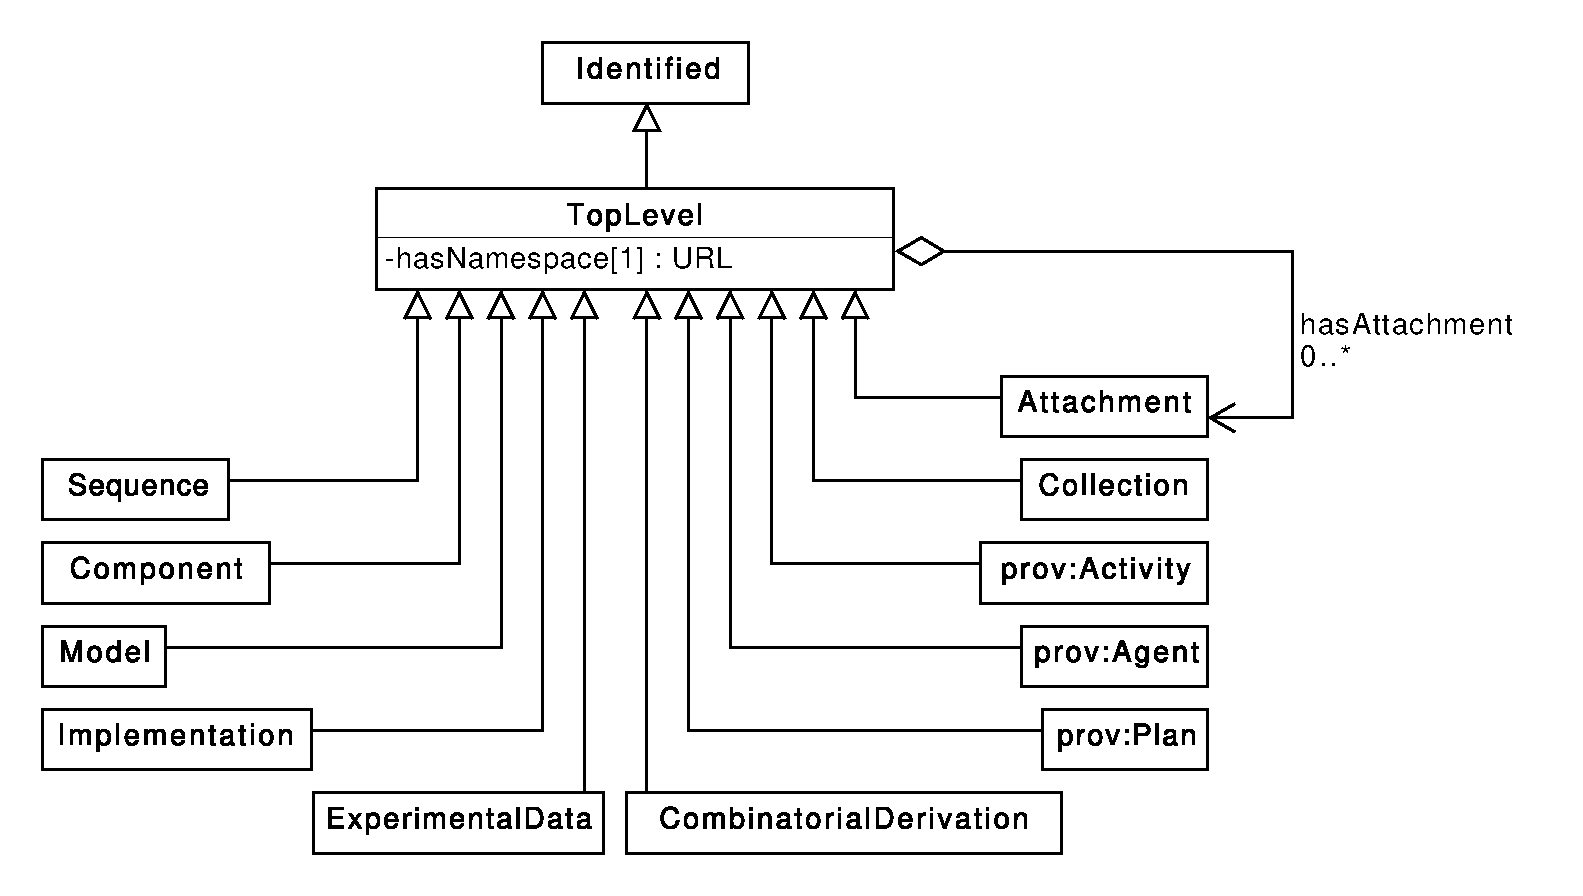
\includegraphics[width=\textwidth]{uml/toplevel}
\caption[]{Classes that inherit from the \sbol{TopLevel} abstract class.}
\label{uml:toplevel}
\end{center}
\end{figure}

\subparagraph{The hasNamespace property}
\label{sec:hasNamespace}
A \sbol{TopLevel} object MUST have precisely one \sbol{hasNamespace} property, which contains a \sbol{URI} that defines the namespace portion of URLs for this object and any child objects.
If the URI for the \sbol{TopLevel} object is a URL, then the URI of the \sbol{hasNamespace} property MUST prefix match that URL.

Note that the requirement for a \sbol{hasNamespace} property holds even for objects with URIs that are not URLs, in order to allow them to be copied into datastores that use URLs.  In this case, however, there is no prefix requirement.


\subparagraph{The hasAttachment property}
\label{sec:hasAttachment}
A \sbol{TopLevel} object can have zero or more \sbol{hasAttachment} properties, each of type URI specifying an \sbol{Attachment} object. The \sbol{Attachment} class is described in more detail in~\ref{sec:Attachment}.


\subsection{Sequence}
\label{sec:Sequence}
The purpose of the \sbol{Sequence} class is to represent the primary structure of a \sbol{Component} object and the manner in which it is encoded. This representation is accomplished  by means of the \sbol{elements} property and \sbol{encoding} property (\ref{uml:sequence}).

\begin{figure}[ht]
\begin{center}
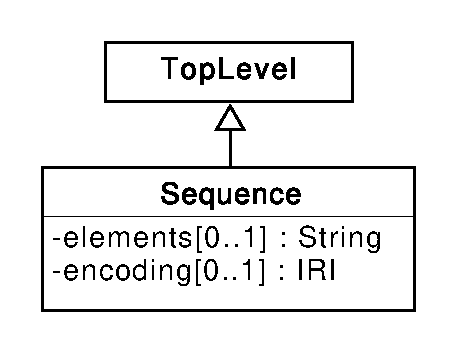
\includegraphics[scale=0.6]{uml/sequence}
\caption[]{Diagram of the \sbol{Sequence} class and its associated properties.}
\label{uml:sequence}
\end{center}
\end{figure}


\subparagraph{The \sbolheading{elements} property}
\label{sec:elements}
The \sbol{elements} property is an OPTIONAL \sbol{String} of characters that represents the constituents of a biological or chemical molecule. 
For example, these characters could represent the nucleotide bases of a molecule of DNA, the amino acid residues of a protein, or the atoms and chemical bonds of a small molecule.

If the \sbol{elements} property is not set, then it means the particulars of this \sbol{Sequence} have not yet been determined.

\subparagraph{The \sbolheading{encoding} property}
\label{sec:encoding}
The \sbol{encoding} property has a data type of \sbol{URI}, and is OPTIONAL unless \sbol{elements} is set, in which case it is REQUIRED.
This property MUST indicate how the \sbol{elements} property of a \sbol{Sequence} are formed and interpreted.

For example, the \sbol{elements} property of a \sbol{Sequence} with an IUPAC DNA encoding property MUST contain characters that represent nucleotide bases, such as {\tt a}, {\tt t}, {\tt c}, and {\tt g}. The \sbol{elements} property of a \sbol{Sequence} with a Simplified Molecular-Input Line-Entry System (SMILES) encoding, on the other hand, MUST contain characters that represent atoms and chemical bonds, such as {\tt C}, {\tt N}, {\tt O}, and {\tt =}.

\ref{tbl:sequence_encodings} provides a list of possible \sbol{URI} values for the \sbol{encoding} property. The terms in \ref{tbl:sequence_encodings} are organized by the type of \sbol{Component} (see \ref{tbl:component_types}) that typically refer to a \sbol{Sequence} with such an \sbol{encoding}. It is RECOMMENDED that the encoding property of a Sequence contains a URI from \ref{tbl:sequence_encodings}. When the \sbol{encoding} of a \sbol{Sequence} is well described by one of the \sbol{URI}s in \ref{tbl:sequence_encodings}, it MUST contain that \sbol{URI}.

More information on IUPAC encoding can be found at \url{http://www.bioinformatics.org/sms2/iupac.html}.

%A Summary of letters for nucleic acids and aminoacids
\begin{table}[ht]
  \begin{edtable}{tabular}{lll}
    \toprule
     \textbf{Encoding} & \textbf{URI} & \textbf{Component Type} \\
    \midrule
     IUPAC DNA, RNA & \url{http://sbols.org/v3#iupacNucleicAcid} & DNA, RNA \\
    IUPAC Protein & \url{http://sbols.org/v3#iupacAminoAcid} & Protein\\
   SMILES & \url{http://www.opensmiles.org/opensmiles.html} & Simple Chemical \\
    \bottomrule
  \end{edtable}
  \caption{\sbol{URI}s for specifying the \sbol{encoding} property of a \sbol{Sequence}, organized by the type of \sbol{Component} (see \ref{tbl:component_types}) that typically refer to a \sbol{Sequence} with such an \sbol{encoding}.}
  \label{tbl:sequence_encodings}
\end{table}


\subsection{Component}
\label{sec:Component}

The \sbol{Component} class represents the structural and/or functional entities of a biological design. The primary usage of this class is to represent entities with designed sequences, such as DNA, RNA, and proteins, but it can also be used to represent any other entity that is part of a design, such as simple chemicals, molecular complexes, strains, media, light, and abstract functional groupings of other entities.

As shown in \ref{uml:component}, the \sbol{Component} class describes a design entity using the following properties: \sbolmult{type:C}{type}, \sbolmult{role:C}{role}, \sbolmult{hasSequence:C}{hasSequence}, \sbol{hasFeature}, \sbol{hasConstraint}, \sbol{hasInteraction}, \sbol{hasInterface}, and \sbol{hasModel}.  
The \sbolmult{hasSequence:C}{hasSequence}, \sbol{hasFeature}, and \sbol{hasConstraint} properties are used to represent structural information, while the\\ \sbol{hasInteraction}, \sbol{hasInterface}, and \sbol{hasModel} are used to represent functional information.

\begin{figure}[ht]
\begin{center}
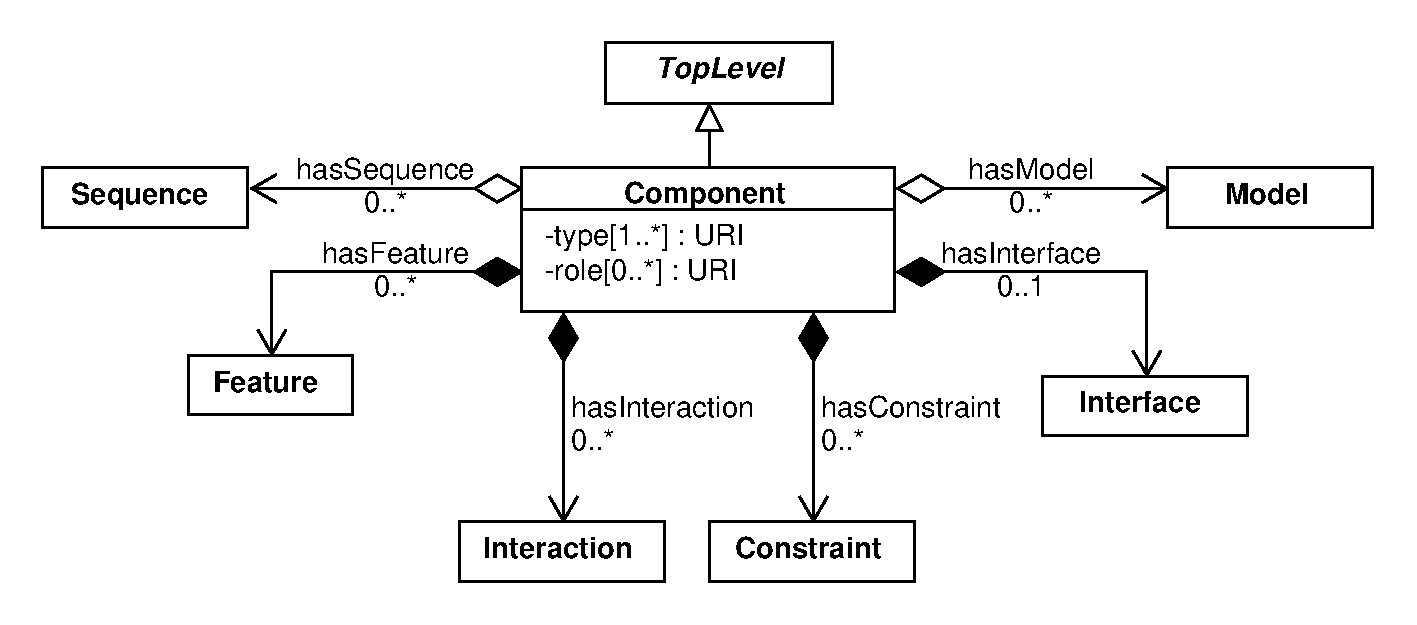
\includegraphics[width=0.95\textwidth]{uml/component}
\caption[]{Diagram of the \sbol{Component} class and its associated properties.}
\label{uml:component}
\end{center}
\end{figure} 

\subparagraph{The \sbolheading{type} property}
\label{sec:type:C}

A \sbol{Component} MUST have one or more \sbolmult{type:C}{type} properties, each of type \sbol{IRI} specifying the category of biochemical or physical entity (for example DNA, protein, or simple chemical) that a \sbol{Component} object abstracts
for the purpose of engineering design. For DNA or RNA entities, additional \sbolmult{type:C}{type} properties MAY be used to describe nucleic acid topology (circular / linear) and strandedness (double- or single-stranded).

The \sbolmult{type:C}{type} properties of every \sbol{Component} MUST include one or more \sbol{IRI}s that MUST identify terms from appropriate ontologies, such as the physical entity representation branch of the Systems Biology Ontology~\cite{SBO} or the ontology of Chemical Entities of Biological Interest (ChEBI)~\cite{chebi}.  
In order to maximize the compatibility of designs, the \sbolmult{type:C}{type} property of a \sbol{Component} SHOULD contain a \sbol{URL} from the physical entity representation branch of the Systems Biology Ontology~\cite{SBO}.
\ref{tbl:component_types} provides a partial list of ontology terms and their \sbol{URL}s,
and any \sbol{Component} that can be well-described by one of the terms in \ref{tbl:component_types} MUST use the \sbol{URL} for that term as a \sbolmult{type:C}{type}.
Finally, if the \sbolmult{type:C}{type} property contains multiple \sbol{IRI}s, then they MUST identify non-conflicting terms (otherwise, it might not be clear how to interpret them). For example, the SBO terms provided by \ref{tbl:component_types} would conflict because they specify classes of biochemical entities with different molecular structures.

\begin{table}[ht]
  \begin{edtable}{tabular}{ll}
    \toprule
    \textbf{Component Type} & \textbf{URL for SBO Term} \\
    \midrule
    DNA (Deoxyribonucleic acid)  & \url{https://identifiers.org/SBO:0000251}\\
    RNA (Ribonucleic acid) & \url{https://identifiers.org/SBO:0000250}\\
    Protein (Polypeptide chain)  & \url{https://identifiers.org/SBO:0000252}\\
    Simple Chemical  & \url{https://identifiers.org/SBO:0000247}\\
    Non-covalent complex  & \url{https://identifiers.org/SBO:0000253}\\
    Functional Entity  & \url{https://identifiers.org/SBO:0000241}\\
    \bottomrule
  \end{edtable}
  \caption{Partial list of the most common SBO terms to specify the molecule type using the \sbolmult{type:C}{type} property of a \sbol{Component}.  Systems of multiple interacting molecules (e.g., a plasmid expressing a protein) should use the functional entity type.}
 \label{tbl:component_types}
\end{table}

\emph{Nucleic Acid Topology types}\\
Any \sbol{Component} classified as DNA (see \ref{tbl:component_types}) is RECOMMENDED to encode circular/linear topology information in an additional \sbolmult{type:C}{type} field. 
This (topology) \sbolmult{type:C}{type} field SHOULD specify a URL from the Topology Attribute branch of the Sequence Ontology (SO): this is currently just `linear' or `circular' as given in \ref{tbl:component_topology}.
Topology information SHOULD be specified for DNA \sbol{Component} records with a fully specified sequence, except in three scenarios: if the DNA record does not have sequence information, or if the DNA record has incomplete sequence information, or if topology is genuinely unknown. 
For any \sbol{Component} classified as RNA (see \ref{tbl:component_types}), a topology type field is OPTIONAL. The default
assumption in this case is linear topology.  
In any case, conflicting topologies MUST NOT be specified.

Any \sbol{Component} classified as DNA or RNA MAY also have strand
information encoded in an additional (third) type field using a URL from the Strand Attribute branch of the SO (currently there are only two possible terms for single or double-stranded nucleic
acids, given in \ref{tbl:component_topology}). In absence of this field, the
default strand information assumed for DNA is `double-stranded' and for RNA is
`single-stranded'. 

Any other type of \sbol{Component} record (protein, simple chemical, etc.) SHOULD NOT
have any type field pointing to SO terms from the topology or strand attribute branches of SO.

Note that a \emph{circular} topology instructs software to interpret the
beginning / end position of a given sequence (be it DNA or RNA) as arbitrary, 
meaning that sequence features MAY be mapped or identified across this junction.
 \emph{Double stranded} instructs software to apply sequence searches to both strands (i.e., sequence and reverse complement of sequence).

\begin{table}[ht]
  \begin{edtable}{tabular}{ll}
    \toprule
    \textbf{Nucleic Acid Topology} & \textbf{URL for Nucleic Acid Topology
      Term in SO} \\
    \midrule
    linear  & \url{http://identifiers.org/SO:0000987}\\
    circular  & \url{http://identifiers.org/SO:0000988}\\
    single-stranded & \url{http://identifiers.org/SO:0000984}\\
    double-stranded & \url{http://identifiers.org/SO:0000985}\\
    \bottomrule
  \end{edtable}
  \caption{Sequence Ontology (SO) terms to encode DNA or RNA topology information in the \sbolmult{type:C}{type} properties of a \sbol{Component}.}
 \label{tbl:component_topology}
\end{table}

\subparagraph{The \sbolheading{role} property}
\label{sec:role:C}

A \sbol{Component} MAY have any number of \sbolmult{role:C}{role} properties, each of type \sbol{IRI}, that MUST identify terms from ontologies that are consistent with the \sbolmult{type:C}{type} property of the \sbol{Component}.  
For example, the \sbolmult{role:C}{role} property of a DNA or RNA \sbol{Component} could contain URLs identifying terms from the Sequence Ontology (SO). As a best practice, a DNA or RNA \sbol{Component} SHOULD contain exactly one \sbol{URL} that refers to a term from the sequence feature branch of the SO.
Similarly, the role properties of a protein and simple chemical \sbol{Component} SHOULD respectively contain \sbol{URL}s identifying terms from the \texttt{MolecularFunction} (\texttt{GO:0003674}) branch of the Gene Ontology (GO) and the \texttt{role} (\texttt{CHEBI:50906}) branch of the CHEBI ontology.
\ref{tbl:component_roles} contains a partial list of possible ontology terms for the \sbolmult{role:C}{role} properties and their \sbol{URL}s. These terms are organized by the type of \sbol{Component} to which they SHOULD apply (see \ref{tbl:component_types}). Any \sbol{Component} that can be well-described by one of the terms in \ref{tbl:component_roles} MUST use the \sbol{URL} for that term as a \sbolmult{role:C}{role}.

These \sbol{IRI}s might identify descriptive biological roles, such as ``metabolic pathway'' and ``signaling cascade,'' but they can also identify identify ``logical'' roles, such as ``inverter'' or ``AND gate'', or other abstract roles for describing the function of design. Interpretation of the meaning of such roles currently depends on the software tools that read and write them.

\begin{table}[ht]
  \begin{edtable}{tabular}{lll}
    \toprule
    \textbf{Component Role} & \textbf{URL for Ontology Term} & \textbf{Component Type} \\
    \midrule
   Promoter & \url{http://identifiers.org/SO:0000167} & DNA \\
   RBS & \url{http://identifiers.org/SO:0000139} & DNA \\
      CDS & \url{http://identifiers.org/SO:0000316} & DNA \\
      Terminator & \url{http://identifiers.org/SO:0000141} & DNA \\
      Gene & \url{http://identifiers.org/SO:0000704} & DNA \\
      Operator & \url{http://identifiers.org/SO:0000057} & DNA \\
      Engineered Region & \url{http://identifiers.org/SO:0000804} & DNA \\
      mRNA & \url{http://identifiers.org/SO:0000234} & RNA \\
      Effector & \url{http://identifiers.org/CHEBI:35224} & Small Molecule \\
      Transcription Factor & \url{http://identifiers.org/GO:0003700} & Protein\\
    \bottomrule
  \end{edtable}
  \caption{Partial list of ontology terms to specify the \sbolmult{role:C}{role} property of a \sbol{Component}, organized by the type of \sbol{Component} to which they are intended to apply (see \ref{tbl:component_types}).}
  \label{tbl:component_roles}
\end{table}

\subparagraph{The \sbolheading{hasSequence} property}
\label{sec:hasSequence:C}
A \sbol{Component} MAY have any number of \sbolmult{hasSequence:C}{hasSequence} properties, each of type \sbol{IRI}, that MUST reference a \sbol{Sequence} object (see \ref{sec:Sequence}).  These objects define the primary structure or structures of the \sbol{Component}.

If a \sbol{Feature} of a \sbol{Component} refers to a \sbol{Location}, and this \sbol{Location} refers to a \sbol{Sequence}, then the \sbol{Component} MUST also include a \sbolmult{hasSequence:C}{hasSequence} property that refers to this \sbol{Sequence}.

Many \sbol{Component} objects will have exactly one \sbolmult{hasSequence:C}{hasSequence} property that refers to a \sbol{Sequence} object.  In this case, if its has a \sbolmult{type:C}{type} from \ref{tbl:component_types} and there is an \sbol{encoding} that is cross-listed with this term in \ref{tbl:sequence_encodings}, then the \sbol{Sequence} objects MUST have this encoding (e.g., a \sbol{Component} of \sbolmult{type:C}{type} DNA must have a \sbol{Sequence} with an IUPAC DNA \sbol{encoding}).
This \sbol{Sequence} is implicitly the entire sequence for this \sbol{Component} (In other words, it is equivalent to a \sbol{SequenceFeature} with an \sbol{EntireSequence} \sbol{Location} that refers to this \sbol{Sequence}).

\subparagraph{The \sbolheading{hasFeature} property}
\label{sec:hasFeature}

A \sbol{Component} MAY have any number of \sbol{hasFeature} properties, each of type \sbol{IRI} that MUST reference a \sbol{Feature} object (see \ref{sec:Feature}). The set of relations between \sbol{Feature} and \sbol{Component} objects MUST be strictly acyclic.

Taking the \sbol{Component} class as analogous to a blueprint or specification sheet for a biological part or a system of interacting biological elements, the \sbol{Feature} class represents the specific occurrence of a part, subsystem, or other notable aspect within that design.  
This mechanism also allows a biological design to include multiple instances of a particular part (defined by reference to the same \sbol{Component}). 
For example, the \sbol{Component} of a polycistronic gene could contain two \sbol{SubComponent} objects that refer to the same \sbol{Component} of a CDS.  
As another example, consider the \sbol{Component} for a network of two-input repressor devices in which the particular repressors have not yet been chosen.
This \sbol{Component} could contain multiple \sbol{SubComponent} objects that refer to the same \sbol{Component} of an abstract two-input repressor device.

The \sbol{hasFeature} properties of \sbol{Component} objects can be used to construct a hierarchy of \sbol{SubComponent} and \sbol{Component} objects.  If a \sbol{Component} in such a hierarchy refers to a \sbol{Location} object, and there exists a \sbol{Component} object lower in the hierarchy that refers to a \sbol{Location} object that refers to the same \sbol{Sequence} with the same \sbol{encoding}, then the \sbol{elements} properties of these \sbol{Sequence} objects SHOULD be consistent with each other, such that well-defined mappings exist from the ``lower level'' \sbol{elements} to the ``higher level'' \sbol{elements} in accordance with their shared \sbol{encoding} properties. This mapping is also subject to any restrictions on the positions of the \sbol{Feature} objects in the hierarchy that are imposed by the \sbol{SubComponent}, \sbol{SequenceFeature}, or \sbol{Constraint} objects contained by the \sbol{Component} objects in the hierarchy.

For example, in a plasmid \sbol{Component} with a promoter \sbol{SubComponent}, the sequence at the promoter's \sbol{Location} within the plasmid should be the sequence for the promoter.
More concretely, consider DNA \sbol{Component} that refers to a \sbol{Sequence} with an \external{IUPAC DNA} \sbol{encoding} and an \sbol{elements} \external{String} of ``{\tt gattaca}.'' In turn, this \sbol{Component} could contain a \sbol{SubComponent} that refers to a ``lower level''  \sbol{Component} that also refers to a \sbol{Sequence} with an \external{IUPAC DNA} \sbol{encoding}. Consequently, a consistent \sbol{elements} \external{String} of this ``lower level'' \sbol{Sequence} could be ``{\tt gatta},'' or perhaps ``{\tt tgta}'' if the \sbol{SubComponent} is positioned by a \sbol{Location} with an \sbolmult{orientation:L}{orientation} of ``reverse complement'' (see \ref{sec:Location}).

\subparagraph{The \sbolheading{hasConstraint} property}
\label{sec:hasConstraint}

A \sbol{Component} MAY have any number of \sbol{hasConstraint} properties, each of type \sbol{IRI}, that MUST reference a \sbol{Constraint} object (see \ref{sec:Constraint}).  
These objects describe, among other things, any restrictions on the relative, sequence-based positions and/or orientations of the \sbol{Feature} objects contained by the \sbol{Component}, as well as spatial relations such as containment and identity relations.
For example, the \sbol{Component} of a gene might specify that the position of its promoter \sbol{SubComponent} precedes that of its CDS \sbol{SubComponent}. This is particularly useful when a \sbol{Component} lacks a \sbol{Sequence} and therefore cannot specify the precise, sequence-based positions of its \sbol{SubComponent} objects using \sbol{Location} objects.

\subparagraph{The \sbolheading{hasInteraction} property}\label{sec:hasInteraction}

A \sbol{Component} MAY have any number of \sbol{hasInteraction} properties, each of type \sbol{IRI}, that MUST reference an \sbol{Interaction} object (see \ref{sec:Interaction}).  

The \sbol{Interaction} class provides an abstract, machine-readable representation of behavior within a \sbol{Component} (whereas a more detailed model of the system might not be suited to machine reasoning, depending on its implementation).
Each \sbol{Interaction} contains \sbol{Participation} objects that indicate the roles of the \sbol{Feature} objects involved in the \sbol{Interaction}.

\subparagraph{The \sbolheading{hasInterface} property}\label{sec:hasInterface}

A \sbol{Component} MAY have zero or one \sbol{hasInterface} property of type \sbol{IRI} that MUST reference an \sbol{Interface} object (see \ref{sec:Interface}).  

An \sbol{Interface} object indicates the inputs, outputs, and non-directional points of connection to a \sbol{Component}.

\subparagraph{The \sbolheading{hasModel} property}\label{sec:hasModel}

A \sbol{Component} MAY have any number of \sbol{hasModel} properties, each of type \sbol{IRI}, that MUST reference a \sbol{Model} object (see \ref{sec:Model}).  

\sbol{Model} objects are placeholders that link \sbol{Component} objects to computational models of any format.
A \sbol{Component} object can link to more than one \sbol{Model} since each might encode system behavior in a different way or at a different level of detail.

\subsubsection{Feature}
\label{sec:Feature}

The \sbol{Feature} class, as shown in \ref{uml:subcomponent} is used to compose \sbol{Component} objects into a structural or functional hierarchy. 
\sbol{Feature} is an abstract class; only its child classes are actually instantiated.

\begin{figure}[ht]
\begin{center}
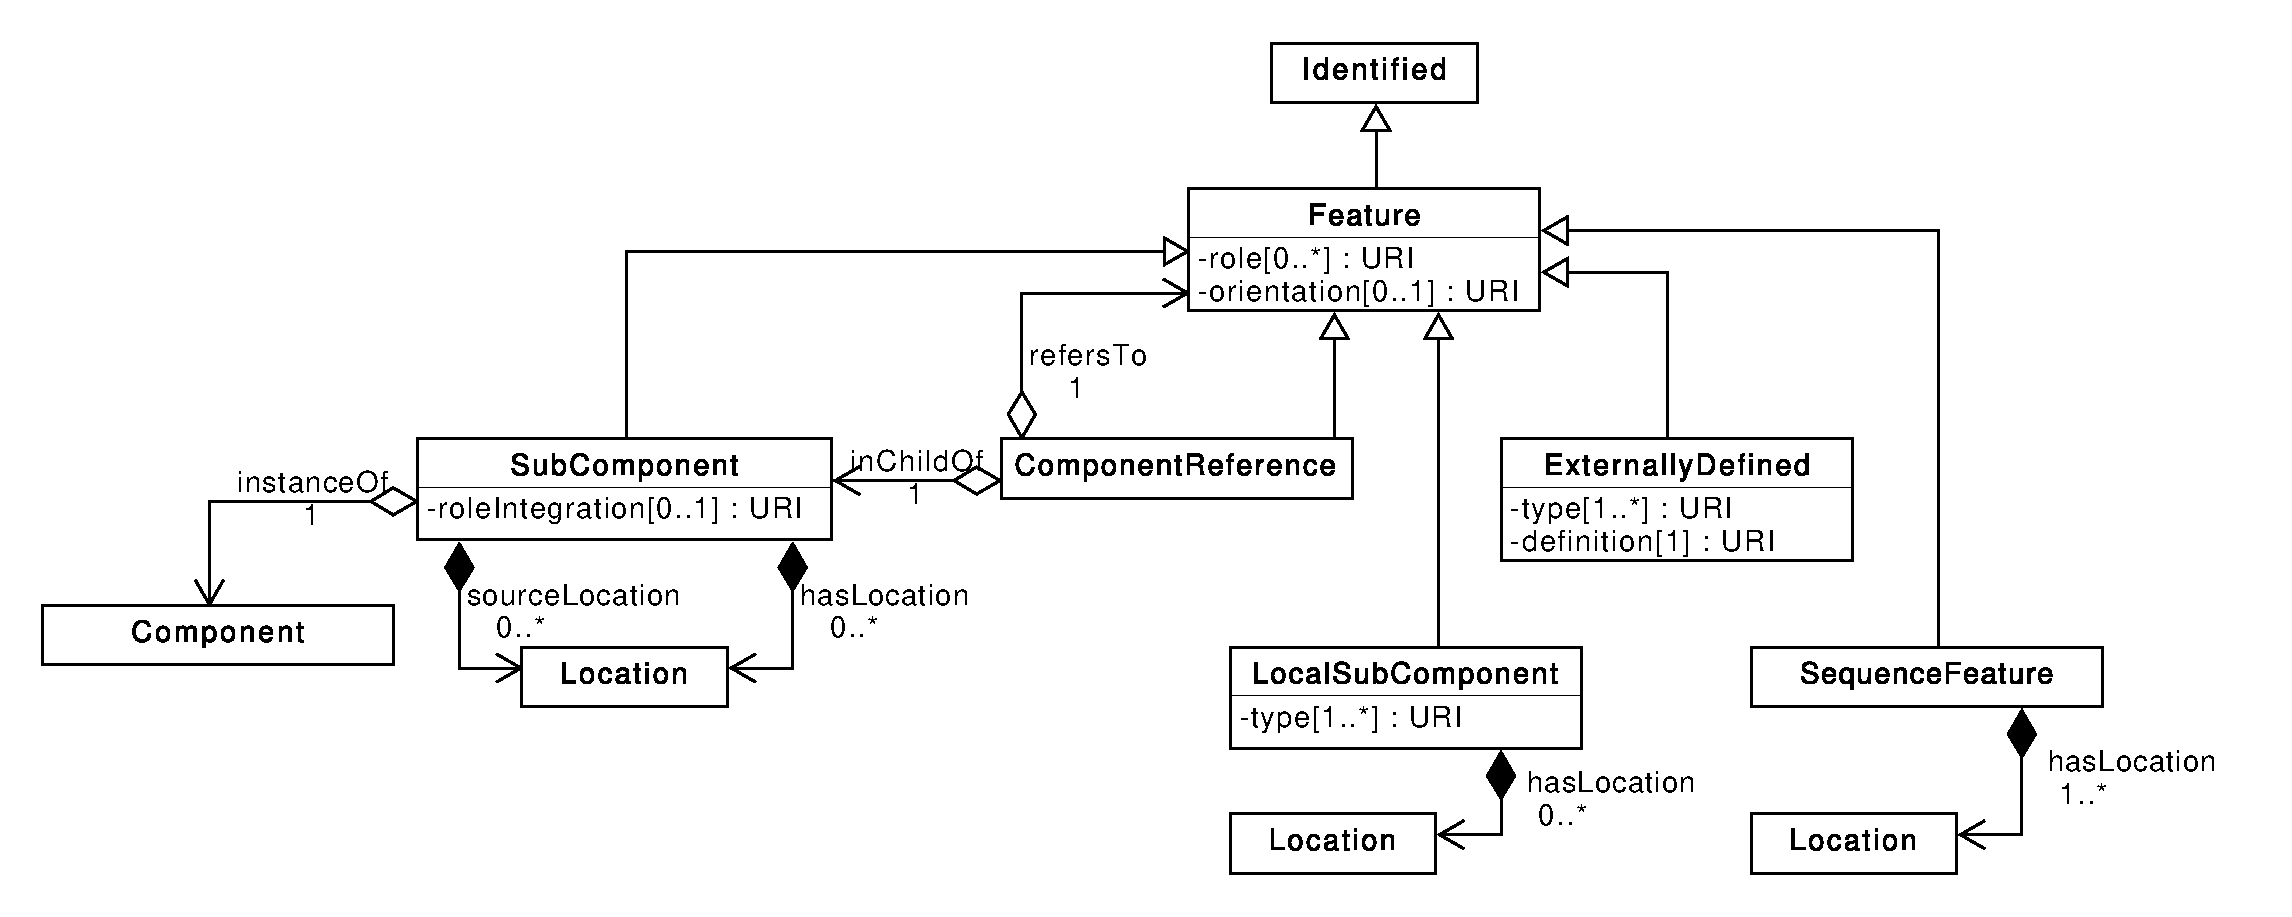
\includegraphics[width=\textwidth]{uml/feature}
\caption[]{Diagram of the \sbol{Feature} class, its children, and associated properties.}
\label{uml:subcomponent}
\end{center}
\end{figure}

\subparagraph{The \sbolheading{role} property}\label{sec:role:F}

Each \sbol{Feature} can have zero or more \sbolmult{role:F}{role} property \sbol{URI}s describing the purpose or potential function of this \sbol{Feature} in the \textit{context} of its parent \sbol{Component}.
If the \sbolmult{role:F}{role} for a \sbol{SubComponent} is left unspecified, then the \sbolmult{role:F}{role} is determined by the \sbolmult{role:C}{role} property of the \sbol{Component} that it is an \sbol{instanceOf}. 
If provided, these \sbolmult{role:F}{role} property \sbol{URI}s MUST identify terms from appropriate ontologies. Roles are not restricted to describing biological function; they may annotate a \sbol{Feature}'s function in any domain for which an ontology exists.
A table of recommended ontology terms for \sbolmult{role:F}{role} is given in \ref{tbl:component_roles}.

It is RECOMMENDED that these \sbolmult{role:F}{role} property \sbol{URI}s identify terms that are compatible with the \sbolmult{type:C}{type} properties of the \sbol{Feature}'s parent \sbol{Component}.
For example, a \sbolmult{role:F}{role} of a \sbol{Feature} which belongs to a \sbol{Component} of type DNA might refer to terms from the Sequence Ontology. 
Likewise, for any feature that is a \sbol{SubComponent}, the \sbolmult{role:F}{role} SHOULD be compatible with the \sbolmult{type:C}{type} of the \sbol{Component} that it links to through its \sbol{instanceOf} property.

\subparagraph{The \sbolheading{orientation} property}
\label{sec:orientation:F}
The \sbolmult{orientation:F}{orientation} property is OPTIONAL and has a data type of \sbol{URI}. This can be used to indicate how any associated double-stranded \sbol{Feature} is oriented on the \sbol{elements} of a \sbol{Sequence} from their parent \sbol{Component}.
If a \sbol{Feature} object has an \sbolmult{orientation:F}{orientation}, then it is RECOMMENDED that it come from \ref{tbl:orientation_types}; for reasons of backwards compatability it MAY instead come from \ref{tbl_orientation_types_alternative}.
 
\begin{table}[ht]
  \begin{edtable}{tabular}{lp{3.75in}}
    \toprule
    \textbf{Orientation URI} & \textbf{Description} \\
    \midrule
    \url{https://identifiers.org/SO:0001030} & The region specified by this \sbol{Feature} or \sbol{Location} is on the \sbol{elements} of a \sbol{Sequence}. \\
    \url{https://identifiers.org/SO:0001031} & The region specified by this \sbol{Feature} or \sbol{Location} is on the reverse-complement mapping of the \sbol{elements} of a \sbol{Sequence}. The exact nature of this mapping depends on the \sbol{encoding} of the \sbol{Sequence}. \\
    \bottomrule
  \end{edtable}
  \caption{RECOMMENDED \sbol{URI}s for the \sbolmult{orientation:F}{orientation} property}
  \label{tbl:orientation_types}
\end{table}



\begin{table}[ht]
  \begin{edtable}{tabular}{lp{3.75in}}
    \toprule
    \textbf{Orientation URI} & \textbf{Description} \\
    \midrule
    \url{http://sbols.org/v3\#inline} & The region specified by this \sbol{Feature} or \sbol{Location} is on the \sbol{elements} of a \sbol{Sequence}. \\
    \url{http://sbols.org/v3\#reverseComplement} & The region specified by this \sbol{Feature} or \sbol{Location} is on the reverse-complement mapping of the \sbol{elements} of a \sbol{Sequence}. The exact nature of this mapping depends on the \sbol{encoding} of the \sbol{Sequence}. \\
    \bottomrule
  \end{edtable}
  \caption{Permitted alternative \sbol{URI}s for the \sbolmult{orientation:F}{orientation} property. The URIS listed in Table~\ref{tbl:orientation_types} are preferred and SHOULD be used instead where possible.}
  \label{tbl:orientation_types_alternative}
\end{table}

\paragraph{SubComponent}
\label{sec:SubComponent}

The \sbol{SubComponent} class is a subclass of the \sbol{Feature} class that can be used to specify structural hierarchy.
For example, the \sbol{Component} of a gene might contain four \sbol{SubComponent} objects: a promoter, RBS, CDS, and terminator, each linked to a \sbol{Component} that provides the complete definition.
In turn, the \sbol{Component} of the promoter \sbol{SubComponent} might itself contain \sbol{SubComponent} objects defining various operator sites, etc.

\subparagraph{The \sbolheading{roleIntegration} property}\label{sec:roleIntegration}

A \sbol{roleIntegration} specifies the relationship between a \sbol{SubComponent} instance's own set of \sbolmult{role:F}{role} properties and the set of \sbolmult{role:C}{role} properties on the included \sbol{Component}.

The \sbol{roleIntegration} property has a data type of \sbol{URI}. A \sbol{SubComponent} instance with zero \sbolmult{role:F}{role} properties MAY OPTIONALLY specify a \sbol{roleIntegration}. A \sbol{SubComponent} instance with one or more \sbolmult{role:F}{role} properties MUST specify a \sbol{roleIntegration} from \ref{tbl:component_roleIntegration}.
If zero \sbol{SubComponent} \sbolmult{role:F}{role} properties are given and no \sbol{SubComponent} \sbol{roleIntegration} is given, then \url{http://sbols.org/v3\#mergeRoles} is assumed.
It is RECOMMENDED to specify \sbol{SubComponent} \sbolmult{role:F}{role} values only if the result would differ from the  \sbolmult{role:C}{role} values belonging to this \sbol{SubComponent}'s included \sbol{Component}.

\begin{table}[ht]
  \begin{edtable}{tabular}{lp{4in}}
    \toprule
    \textbf{roleIntegration URI} & \textbf{Description} \\
    \midrule
    \url{http://sbols.org/v3\#overrideRoles} & In the context of this \sbol{SubComponent}, ignore any \sbolmult{role:C}{role} given for the included \sbol{Component}. Instead use only the set of zero or more \sbolmult{role:F}{role} properties given for this \sbol{SubComponent}. \\
    \url{http://sbols.org/v3\#mergeRoles} & Use the union of the two sets: both the set of zero or more \sbolmult{role:F}{role} properties given for this \sbol{SubComponent} as well as the set of zero or more \sbolmult{role:C}{role} properties given for the included \sbol{Component}. \\
    \bottomrule
  \end{edtable}
  \caption{Each \sbol{roleIntegration} mode is associated with a rule governing how a \sbol{SubComponent}'s \sbolmult{role:F}{role} values are to be combined with the included \sbol{Component}'s \sbolmult{role:C}{role} values.}
  \label{tbl:component_roleIntegration}
\end{table}

\subparagraph{The \sbolheading{instanceOf} property}
\label{sec:instanceOf}

The \sbol{instanceOf} property is a REQUIRED \sbol{URI} that refers to the \sbol{Component} providing the definition for this \sbol{SubComponent}.
Among other things, as described in the previous section, this \sbol{Component} effectively provides information about the \sbolmult{type:C}{type} and \sbolmult{role:C}{role} of the \sbol{SubComponent}.

The \sbol{instanceOf} property MUST NOT refer to the same \sbol{Component} as the one that contains the \sbol{SubComponent}.
Furthermore, \sbol{SubComponent} objects MUST NOT form a cyclical chain of references via their \sbol{instanceOf} properties and the \sbol{Component} objects that contain them.
For example, consider the \sbol{SubComponent} objects $A$ and $B$ and the \sbol{Component} objects $X$ and $Y$. The reference chain ``$X$ has feature $A$, $A$ is an instance of $Y$, $Y$ has feature $B$, and $B$ is an instance of $X$'' is cyclical.


\subparagraph{The \sbolheading{hasLocation} property}\label{sec:hasLocation:SC}

A \sbol{SubComponent} MAY have any number of \sbolmult{hasLocation:SC}{hasLocation} properties, each of type \sbol{URI}, that MUST refer to \sbol{Location} objects that indicates the location of the \sbol{Sequence} from the \sbol{instanceOf} \sbol{Component} in a \sbol{Sequence} of the parent \sbol{Component}.

If any \sbolmult{hasLocation:SC}{hasLocation} is defined, then there MUST BE precisely one \sbol{Sequence} in the \sbol{instanceOf} \sbol{Component}, as otherwise this relationship is ill-defined.

If no \sbolmult{hasLocation:SC}{hasLocation} is defined, this indicates a part / sub-part relationship for which sequence details have not (yet) been determined or involving types for which sequence relationships are not relevant (e.g., inclusion of a reaction chain within a larger metabolic network).

Allowing multiple \sbol{Location} objects on a single \sbol{SubComponent} is intended to enable representation of discontinuous regions (for example, a coding sequence encoded across a set of exons with interspersed introns).
As such, the \sbol{Location} objects of a single \sbol{SubComponent} MUST NOT specify overlapping regions, since it is not clear what this would mean.
There is no such concern with different objects, however, which can freely overlap in \sbol{Location} (for example, specifying overlapping linkers for sequence assembly).


\subparagraph{The \sbolheading{sourceLocation} property}\label{sec:sourceLocation}

The \sbol{sourceLocation} property allows for only a portion of a \sbol{Component}'s \sbol{Sequence} to be included, rather than its entirety.
For example, when composing parts with certain assembly methods, some bases on the boundary may be removed or replaced.
Another example is describing a deletion or replacement of a portion of a sequence.

A \sbol{SubComponent} MAY have any number of \sbol{sourceLocation} properties, each of type \sbol{URI}, that MUST refer to  \sbol{Location} objects that indicate which \sbol{elements} of the \sbol{instanceOf} \sbol{Component}'s \sbol{Sequence} are used in defining the parent of the \sbol{SubComponent}.

If there are no \sbol{sourceLocation} properties, then the whole \sbol{Sequence} is assumed to be included. 


\paragraph{ComponentReference}
\label{sec:ComponentReference}

The \sbol{ComponentReference} class is a subclass of \sbol{Feature} that can be used to reference \sbol{Feature}s within\\ \sbol{SubComponent}s. 

\subparagraph{The \sbolheading{inChildOf} property}\label{sec:inChildOf}

The \sbol{inChildOf} property is a REQUIRED \sbol{URI} that refers to a \sbol{SubComponent}. 
The \sbol{inChildOf} property MUST refer to a \sbol{SubComponent} pointed directly to by the parent of the \sbol{ComponentReference}.
Specifically:
\begin{itemize}
\item If the parent of the \sbol{ComponentReference} is a \sbol{Component}, then \sbol{inChildOf} MUST be one of its \sbol{SubComponent}s.
\item If the parent of the \sbol{ComponentReference} is another \sbol{ComponentReference}, then \sbol{inChildOf} MUST be a \sbol{SubComponent} of the \sbol{Component} linked as \sbol{instanceOf} the parent's \sbol{inChildOf} \sbol{SubComponent}.
\end{itemize}

\subparagraph{The \sbolheading{refersTo} property}\label{sec:refersTo}

The \sbol{refersTo} property is a REQUIRED \sbol{URI} that refers to a \sbol{Feature}.

This can be used to either link to the \sbol{Feature} being referenced or to chain hierarchically through additional layers of \sbol{SubComponent}.
\begin{itemize}
\item If the \sbol{Feature} is a \sbol{ComponentReference}, then that \sbol{ComponentReference} acts as a hierarchical link in a chain of references, and MUST be either a child of the \sbol{ComponentReference} linking to it via \sbol{refersTo} or a child of the \sbol{Component} linked as \sbol{instanceOf} the \sbol{ComponentReference}'s \sbol{inChildOf} \sbol{SubComponent}.
\item Otherwise, if the \sbol{refersTo} refers to any other type of \sbol{Feature}, that \sbol{Feature} MUST be a child of the \sbol{Component} linked as \sbol{instanceOf} the \sbol{ComponentReference}'s \sbol{inChildOf} \sbol{SubComponent}.
\end{itemize}

For example, \sbol{ComponentReference} R1 looking into a \sbol{SubComponent} for a plasmid might link with \sbol{refersTo} to its own child \sbol{ComponentReference} R2, which in turn looks within the \sbol{Component} defining the plasmid to the plasmid's CDS \sbol{SubComponent}, in turn using \sbol{refersTo} to reference a \sbol{SequenceFeature} within the \sbol{Component} that defines that CDS.

\paragraph{LocalSubComponent}
\label{sec:LocalSubComponent}

The \sbol{LocalSubComponent} class is a subclass of \sbol{Feature}. 
This class serves as a way to create a placeholder in more complex \sbol{Component}s, such as a variable to be filled in later or a composite that exists only within the context of the parent \sbol{Component}.

\subparagraph{The \sbolheading{type} property}\label{sec:type:LSC}

The \sbolmult{type:LSC}{type} property is REQUIRED and contains one or more \sbol{URI}s. The \sbolmult{type:LSC}{type} property is identical to its use in \sbol{Component}.

\subparagraph{The \sbolheading{hasLocation} property}\label{sec:hasLocation:LSC}

A \sbol{LocalSubComponent} MAY have any number of \sbolmult{hasLocation:LSC}{hasLocation} properties, each of type \sbol{URI}, that MUST refer to \sbol{Location} objects. 
These follow the same restrictions as for the \sbolmult{hasLocation:SC}{hasLocation} of a \sbol{SubComponent}, notably that the \sbol{Location}s of \sbolmult{hasLocation:LSC}{hasLocation} properties attached to the same \sbol{LocalSubComponent} MUST NOT overlap.

\paragraph{ExternallyDefined}
\label{sec:ExternallyDefined}

The \sbol{ExternallyDefined} class has been introduced so that external definitions in databases like ChEBI or UniProt can be referenced.

\subparagraph{The \sbolheading{type} property}\label{sec:type:ED}

The \sbolmult{type:ED}{type} property is REQUIRED and contains one or more \sbol{URI}s. The \sbolmult{type:ED}{type} property is identical to its use in \sbol{Component}.

\subparagraph{The \sbolheading{definition} property}\label{sec:definition:ED}

The \sbolmult{definition:ED}{definition} property is REQUIRED and is of type \sbol{URI} that links to a canonical definition external to SBOL.
When possible, such definitions SHOULD use the recommended external resources in \ref{sec:recomm_ontologies}.
For example, an \sbol{ExternallyDefined} simple chemical might link to ChEBI and a protein might link to UniProt.

\paragraph{SequenceFeature}
\label{sec:SequenceFeature}

The \sbol{SequenceFeature} class describes one or more regions of interest on the \sbol{Sequence} objects referred to by its parent \sbol{Component}. 

\subparagraph{The \sbolheading{hasLocation} property}\label{sec:hasLocation:SF}

The \sbolmult{hasLocation:SF}{hasLocation} is REQUIRED and contains one or more \sbol{URI}s, which MUST refer to \sbol{Location} objects. 
These follow the same restrictions as for the \sbolmult{hasLocation:SC}{hasLocation} of a \sbol{SubComponent}, notably that the \sbol{Location}s of \sbolmult{hasLocation:SF}{hasLocation} properties attached to the same \sbol{SequenceFeature} MUST NOT overlap.



\subsubsection{Location}
\label{sec:Location}

The \sbol{Location} class (as shown in \ref{uml:location}) is used to represent the location of \sbol{Feature}s within \sbol{Sequence}s.  This class is extended by the \sbol{Range}, \sbol{Cut}, and \sbol{EntireSequence} classes
\sbol{Location} is an abstract class; only its child classes are actually instantiated.

\begin{figure}[ht]
\begin{center}
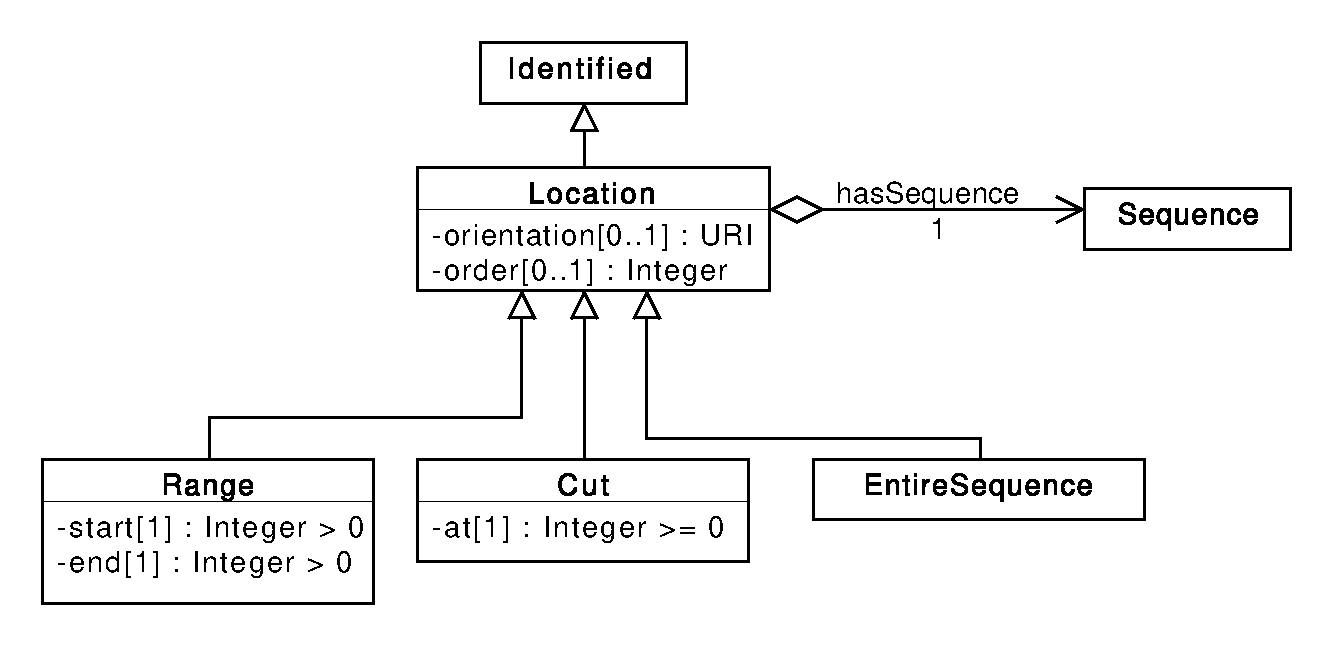
\includegraphics[scale=0.6]{uml/location}
\caption[]{Diagram of the \sbol{Location} class and its associated properties.}
\label{uml:location}
\end{center}
\end{figure} 

\subparagraph{The \sbolheading{orientation} property}
\label{sec:orientation:L}
The \sbolmult{orientation:L}{orientation} property is OPTIONAL and has a data type of \sbol{URI}. All subclasses of \sbol{Location} share this property, which can be used to indicate how any associated double-stranded \sbol{Feature} is oriented on the \sbol{elements} of a \sbol{Sequence} from their parent \sbol{Component}.
If a \sbol{Location} object has an \sbolmult{orientation:F}{orientation}, then it is RECOMMENDED that it come from \ref{tbl:orientation_types}; for reasons of backwards compatability it MAY instead come from \ref{tbl_orientation_types_alternative}.


As is typical practice in biology, any change in orientation is applied after indices are interpreted.
Thus, for example, in a DNA \sbol{Sequence} with \sbol{elements} {\tt AAAAACCCCCTTTTTGGGGGTTTTTGGGGG}, 
indices 1-6 with a reverse orientation will select {\tt AAAAAC}, which would then be reverse complemented to obtain {\tt GTTTTT}.

\subparagraph{The \sbolheading{order} property}
\label{sec:order}
The \sbol{order} property is OPTIONAL and has a data type of \sbol{Integer}.  If there are multiple \sbol{Location} objects associated with a \sbol{Feature}, the \sbol{order} property is used to specify the order (in increasing value) in which the specified \sbol{Location}s are to be joined to form the sequence of the \sbol{Feature}.
Note that order values MAY be non-sequential and non-positive, if desired.

\subparagraph{The \sbolheading{hasSequence} property}
\label{sec:hasSequence:L}
The \sbolmult{hasSequence:L}{hasSequence} property is REQUIRED and MUST contain the \sbol{URI} of a \sbol{Sequence} object. All subclasses of \sbol{Location} share this property, which indicates which \sbol{Sequence} object referenced by the containing \sbol{Component} is referenced by the \sbol{Location}.

\paragraph{Range}
\label{sec:Range}
A \sbol{Range} object specifies a region via discrete, inclusive \sbol{start} and \sbol{end} positions that correspond to indices for characters in the \sbol{elements} \sbol{String} of a \sbol{Sequence}.

Note that the index of the first location is 1, as is typical practice in biology, rather than 0, as is typical practice in computer science.

\subparagraph{The \sbolheading{start} property}\label{sec:start}
The \sbol{start} property specifies the inclusive starting position of the \sbol{Range}. This property is REQUIRED and MUST contain an \sbol{Integer} value greater than zero.

\subparagraph{The \sbolheading{end} property}\label{sec:end}
The \sbol{end} property specifies the inclusive ending position of the \sbol{Range}. This property is REQUIRED and MUST contain an \sbol{Integer} value greater than zero. In addition, this \sbol{Integer} value MUST be greater than or equal to that of the \sbol{start} property.

\paragraph{Cut}
\label{sec:Cut}
The \sbol{Cut} class has been introduced to enable the specification of a region between two discrete positions.
This specification is accomplished using the \sbol{at} property, which specifies a discrete position that corresponds to the index of a character in the \sbol{elements} \sbol{String} of a \sbol{Sequence} (except in the case when \sbol{at} is equal to zero---see below).

\subparagraph{The \sbolheading{at} property}
\label{sec:at}
The \sbol{at} property is REQUIRED and MUST contain an \sbol{Integer} value greater than or equal to zero. The region specified by the \sbol{Cut} is between the position specified by this property and the position that immediately follows it. When the \sbol{at} property is equal to zero, the specified region is immediately before the first discrete position or character in the \sbol{elements} \sbol{String} of a \sbol{Sequence}.


\paragraph{EntireSequence}
\label{sec:EntireSequence}
The \sbol{EntireSequence} class does not have any additional properties. Use of this class indicates that the linked Sequence describes the entirety of the \sbol{Component} or \sbol{Feature} parent of this Location object.




\subsubsection{Constraint}
\label{sec:Constraint}
The \sbol{Constraint} class can be used to assert restrictions on the relationships of pairs of \sbol{Feature} objects contained by the same parent \sbol{Component}.
Uses of this class include expressing containment (e.g., a plasmid transformed into a chassis strain), identity mappings (e.g., replacing a placeholder value with a complete definition), and expressing relative, sequence-based positions (e.g., the ordering of features within a template).
Each \sbol{Constraint} includes the \sbol{subject}, \sbol{object}, and \sbol{restriction} properties.

\begin{figure}[ht]
\begin{center}
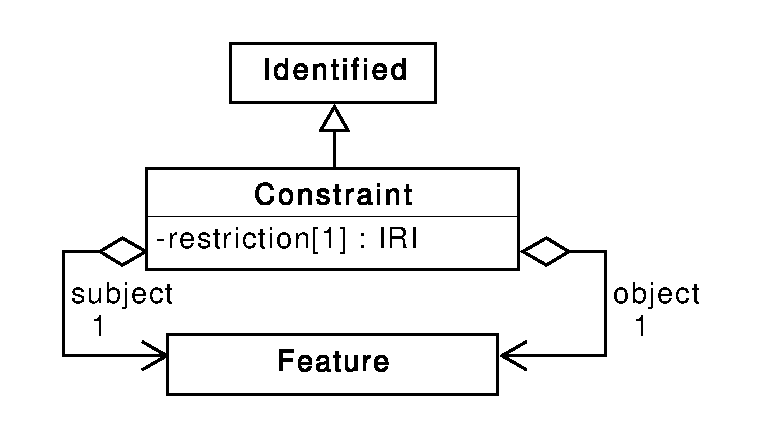
\includegraphics[scale=0.6]{uml/constraint}
\caption[]{Diagram of the \sbol{Constraint} class and its associated properties.}
\label{uml:sequence_constraint}
\end{center}
\end{figure}

\subparagraph{The \sbolheading{subject} property}\label{sec:subject}
The \sbol{subject} property is REQUIRED and MUST contain a \sbol{URI} that refers to a \sbol{Feature} contained by the same parent \sbol{Component} that contains the \sbol{Constraint}.

\subparagraph{The \sbolheading{object} property}\label{sec:object}
The \sbol{object} property is REQUIRED and MUST contain a \sbol{URI} that refers to a \sbol{Feature} contained by the same parent \sbol{Component} that contains the \sbol{Constraint}. This \sbol{Feature} MUST NOT be the same \sbol{Feature} that the \sbol{Constraint} refers to via its \sbol{subject} property.

\subparagraph{The \sbolheading{restriction} property}\label{sec:restriction}

The \sbol{restriction} property is REQUIRED and has a data type of \sbol{URI}. 
This property MUST indicate the type of restriction on the locations, orientations, or identities of the \sbol{subject} and \sbol{object} \sbol{Feature} objects in relation to each other. 
The \sbol{URI} value of this property SHOULD come from the RECOMMENDED \sbol{URI}s in \ref{tbl:restriction_types_identity}, \ref{tbl:restriction_types_topology}, and \ref{tbl:restriction_types_sequence}.

% identify and orientation
\begin{table}[ht]
  \begin{edtable}{tabular}{lp{3.25in}}
    \toprule
    \textbf{Restriction URI} & \textbf{Description} \\
    \midrule
    % identity relations
	\url{http://sbols.org/v3#verifyIdentical}  & The \sbol{subject} and \sbol{object}, after tracing through any layers of \sbol{ComponentReference}, MUST both refer to \sbol{SubComponent} objects with the same \sbol{instanceOf} value or both refer to \sbol{ExternallyDefined} objects with the same \sbolmult{definition:ED}{definition}.
	\emph{Example: a promoter included via two different subsystems must be the identical.} \\
	\url{http://sbols.org/v3\#differentFrom} & The \sbol{subject} and \sbol{object}, after tracing through any layers of \sbol{ComponentReference}, MUST NOT both refer to \sbol{SubComponent} objects with the same \sbol{instanceOf} value or both refer to \sbol{ExternallyDefined} objects with the same \sbolmult{definition:ED}{definition}.
	\emph{Example: two fluorescent reporters must be different.}\\
	\url{http://sbols.org/v3#replaces} &	In the context of the parent object of the \sbol{Constraint}, information about the \sbol{subject} should be used in place of all instances of the \sbol{object}. \emph{Example: the J23101 promoter replaces a generic promoter.} \\
    
    % orientation relations
	\url{http://sbols.org/v3\#sameOrientationAs} & The \sbol{subject} and \sbol{object} \sbol{Component} objects MUST have the same orientation. \emph{Example: a promoter has the same orientation as the coding sequence it controls.}\\
	\url{http://sbols.org/v3\#oppositeOrientationAs} & The \sbol{subject} and \sbol{object} \sbol{Component} objects MUST have opposite orientations. \emph{Example: a promoter has the opposite orientation as an invertase-activated coding sequence it controls.}\\

    \bottomrule
  \end{edtable}
  \caption{RECOMMENDED \sbol{URI}s for expressing identity and orientation with the \sbol{restriction} property.}
  \label{tbl:restriction_types_identity}
\end{table}

    % topology relations
\begin{table}[ht]
  \begin{edtable}{tabular}{lp{3.25in}}
    \toprule
    \textbf{Restriction URI} & \textbf{Description} \\
    \midrule
	\url{http://sbols.org/v3#isDisjointFrom}	& The \sbol{subject} and \sbol{object} do not overlap in space. \emph{Example: a plasmid is disjoint from a chromosome.} \\
	\url{http://sbols.org/v3#strictlyContains} &	The \sbol{subject} entirely contains the \sbol{object}: they do not share a boundary. \emph{Example: a cell contains a plasmid} \\
	\url{http://sbols.org/v3#contains} &	The \sbol{subject} contains the \sbol{object} and they might or might not share a boundary (i.e., union of {\tt strictlyContains}, {\tt equals}, and {\tt covers}. \emph{Example: a cell contains a protein that may or may not bind to its membrane.} \\
	\url{http://sbols.org/v3#equals} &	The \sbol{subject} and \sbol{object} occupy the same location in space. \emph{Example: a small molecule is distributed throughout an entire sample.} \\
	\url{http://sbols.org/v3#meets} &	The \sbol{subject} and \sbol{object} are connected at a shared boundary. \emph{Example: two strains of adherent cells meet at their membranes.} \\
	\url{http://sbols.org/v3#covers} &	The \sbol{subject} contains the \sbol{object} but also shares a boundary. \emph{Example: a cell covers its transmembrane proteins.} \\
	\url{http://sbols.org/v3#overlaps} &	The \sbol{subject} and \sbol{object} overlap in space, but portions of each are outside of the other. \emph{Example: a transmembrane protein overlaps the cell membrane.} \\
    \bottomrule
  \end{edtable}
  \caption{RECOMMENDED \sbol{URI}s for expressing topological relations with the \sbol{restriction} property.}
  \label{tbl:restriction_types_topology}
\end{table}

\begin{table}[ht]
  \begin{edtable}{tabular}{lp{3.25in}}
    \toprule
    \textbf{Restriction URI} & \textbf{Description} \\
    \midrule
    % linear relations
	\url{http://sbols.org/v3#precedes} &	The start of the location for \sbol{subject} is less than the start of the location for \sbol{object} (i.e., union of {\tt strictlyPrecedes}, {\tt meets}, and {\tt overlaps}). 
	\emph{Example: a promoter precedes a ribosome entry site, but the exact boundary between the two will be determined by sequence optimization and assembly planning}. \\
	
	\url{http://sbols.org/v3#strictlyPrecedes} &	The end of the location for \sbol{subject} is less than the start of the location for \sbol{object}. 
	\emph{Example: a promoter strictly precedes a terminator (with a CDS between them).} \\
	
	\url{http://sbols.org/v3#meets} &	The end of the location for \sbol{subject} is equal to the start of the location for \sbol{object}. 
	Note: this is a stronger interpretation of {\tt meets} from \ref{tbl:restriction_types_topology} in the context of a linear sequence.
	\emph{Example: the 3' region adjacent to a blunt restriction site meets the 5' region adjacent to the site.} \\
	
	\url{http://sbols.org/v3#overlaps} &	The start of the location for \sbol{subject} is before the start of the location for \sbol{object} and the end of the location for \sbol{subject} is before the end of the location for \sbol{object}. 
	Note: this is a stronger interpretation of {\tt overlaps} from \ref{tbl:restriction_types_topology} in the context of a linear sequence.
	\emph{Example: two adjacent oligos overlap in a Gibson assembly plan.} \\
	
	\url{http://sbols.org/v3#contains} &	The start of the location for \sbol{subject} is less than or equal to the start of the location for \sbol{object} and the end of the location for \sbol{subject} is greater than or equal to the end of the location for \sbol{object} (i.e., union of {\tt strictlyContains}, {\tt equals}, {\tt finishes}, and {\tt starts}). 
	Note: this is a stronger interpretation of {\tt contains} from \ref{tbl:restriction_types_topology} in the context of a linear sequence.
	\emph{Example: a composite part contains a promoter.} \\
	
	\url{http://sbols.org/v3#strictlyContains} &	The start of the location for \sbol{subject} is before the start of the location for \sbol{object} and the end of the location for \sbol{subject} is after the end of the location for \sbol{object}. 
	Note: this is a stronger interpretation of {\tt strictlyContains} from \ref{tbl:restriction_types_topology} in the context of a linear sequence.
	\emph{Example: an RNA transcript strictly contains an intron.} \\
	
	\url{http://sbols.org/v3#equals} &	The start and end of the location for \sbol{subject} are equal to the start and end of the location for \sbol{object}. 
	Note: this is a stronger interpretation of {\tt equals} from \ref{tbl:restriction_types_topology} in the context of a linear sequence.
	\emph{Example: the transcribed region of a CDS part equals the entire part.} \\
	
	\url{http://sbols.org/v3#finishes} &	The start of the location for \sbol{subject} is after the start of the location for \sbol{object} and the end of the location for \sbol{subject} is equal to the end of the location for \sbol{object}. 
	\emph{Example: a terminator finishes an expression cassette.} \\
	
	\url{http://sbols.org/v3#starts} &	The start of the location for \sbol{subject} is equal to the start of the location for \sbol{object} and the end of the location for \sbol{subject} is before the end of the location for \sbol{object}. 
	\emph{Example: a promoter starts an expression cassette.} \\
    \bottomrule
  \end{edtable}
  \caption{RECOMMENDED \sbol{URI}s for expressing sequential relations with the \sbol{restriction} property. 
  Note that these relations are only well-defined when the \sbol{subject} and \sbol{object} can be located on the same \sbol{Sequence} (though this may be something that is inferred rather than known {\it a priori}).
  In interpreting these relations, it is important to remember that for \sbol{Range} objects, the \sbol{start} and \sbol{end} indices refer to whole bases/residues such that a \sbol{Range} with \sbol{end} equal to 9 \external{meets}  a \sbol{Range} with \sbol{start} equal to 10, while it \external{strictlyPrecedes} a \sbol{Cut} with \sbol{at} equal to 10.
}
  \label{tbl:restriction_types_sequence}
\end{table}




\subsubsection{Interaction}
\label{sec:Interaction}

The \sbol{Interaction} class (as shown in \ref{uml:interaction}) provides more detailed description of how the \sbol{Feature} objects of a \sbol{Component} are intended to work together.  
For example, this class can be used to represent different forms of genetic regulation (e.g., transcriptional activation or repression), processes from the central dogma of biology (e.g. transcription and translation), and other basic molecular interactions (e.g., non-covalent binding or enzymatic phosphorylation).
Each \sbol{Interaction} includes \sbolmult{type:I}{type} properties that refer to descriptive ontology terms and \sbol{hasParticipation} properties that describe which \sbol{Feature} objects participate in which ways in the \sbol{Interaction}.

\begin{figure}[ht]
\begin{center}
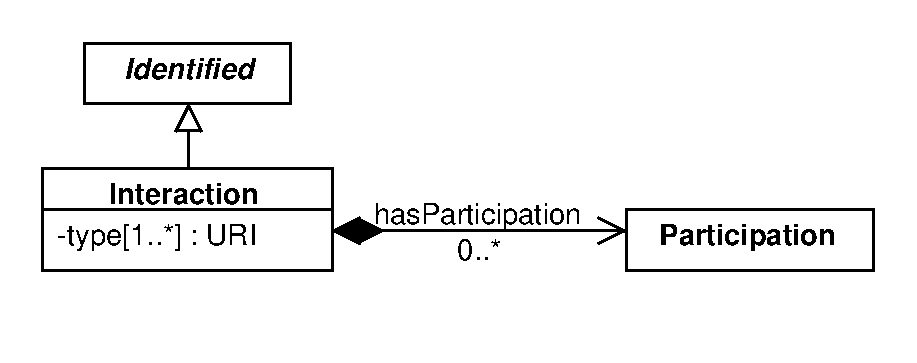
\includegraphics[scale=0.6]{uml/interaction}
\caption[]{Diagram of the \sbol{Interaction} class and its associated properties.}
\label{uml:interaction}
\end{center}
\end{figure}

\subparagraph{The \sbolheading{type} property}\label{sec:type:I}

An \sbol{Interaction} is REQUIRED to have one or more \sbolmult{type:I}{type} properties, each of type \sbol{URI}, that describes the behavior represented by an \sbol{Interaction}.

Each \sbolmult{type:I}{type} property MUST identify terms from appropriate ontologies. 
It is RECOMMENDED that exactly one \sbol{URI} specified by a \sbolmult{type:I}{type} property refer to a term from the occurring entity branch of the \href{http://www.ebi.ac.uk/sbo/main/}{Systems Biology Ontology (SBO)}.
\ref{tbl:interaction_types} provides a partial list of possible SBO terms for the \sbolmult{type:I}{type} property and their corresponding \sbol{URI}s.

\begin{table}[ht]
  \begin{edtable}{tabular}{ll}
    \toprule
    \textbf{Interaction Type} & \textbf{URI for SBO Term} \\
    \midrule
    Inhibition  & \url{http://identifiers.org/biomodels.sbo/SBO:0000169}\\
    Stimulation & \url{http://identifiers.org/biomodels.sbo/SBO:0000170}\\
    Biochemical Reaction & \url{http://identifiers.org/biomodels.sbo/SBO:0000176}\\
    Non-Covalent Binding & \url{http://identifiers.org/biomodels.sbo/SBO:0000177}\\
    Degradation & \url{http://identifiers.org/biomodels.sbo/SBO:0000179}\\
    Genetic Production & \url{http://identifiers.org/biomodels.sbo/SBO:0000589}\\
    Control  & \url{http://identifiers.org/biomodels.sbo/SBO:0000168} \\
    \bottomrule
  \end{edtable}
  \caption{Partial list of SBO terms to specify the \sbolmult{type:I}{type} property of an \sbol{Interaction}.}
  \label{tbl:interaction_types}
\end{table}

If an \sbol{Interaction} is well described by one of the terms from \ref{tbl:interaction_types}, then a \sbolmult{type:I}{type} property MUST refer to the \sbol{URI} that identifies this term. Lastly, if there are multiple \sbolmult{type:I}{type} properties for an \sbol{Interaction}, then they MUST identify non-conflicting terms. For example, the SBO terms ``stimulation'' and ``inhibition'' would conflict.

\subparagraph{The \sbolheading{hasParticipation} property}\label{sec:hasParticipation}

An \sbol{Interaction} MAY have any number of \sbol{hasParticipation} properties, each of type \sbol{URI}, that MUST reference a \sbol{Participation} object, each of which identifies the \sbolmult{role:P}{role} that its referenced \sbol{Feature} plays in the \sbol{Interaction}.

Even though an \sbol{Interaction} generally contains at least one \sbol{Participation}, the case of zero \sbol{Participation} objects is allowed because it is plausible that a designer might want to specify that an \sbol{Interaction} will exist, even if its \sbol{participant}s have not yet been determined.


\paragraph{Participation}
\label{sec:Participation}

Each \sbol{Participation} (see \ref{uml:participation}) represents how a particular \sbol{Feature} behaves in its parent \sbol{Interaction}.

\begin{figure}[ht]
\begin{center}
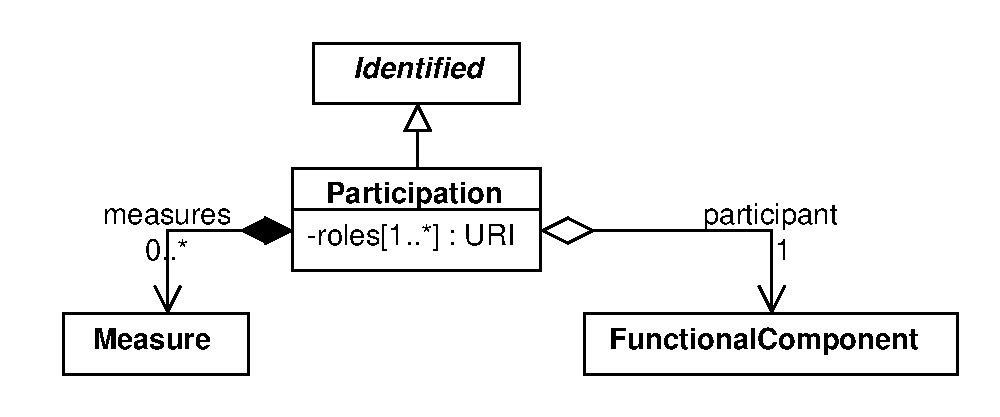
\includegraphics[scale=0.6]{uml/participation}
\caption[]{Diagram of the \sbol{Participation} class and its associated properties.}
\label{uml:participation}
\end{center}
\end{figure}

\subparagraph{The \sbolheading{role} property}\label{sec:role:P}

A \sbol{Participation} is REQUIRED to have one or more \sbolmult{role:P}{role} properties, each of type \sbol{URI}, that describes the behavior of a \sbol{Participation} (and by extension its referenced \sbol{Feature}) in the context of its parent \sbol{Interaction}.

Each \sbolmult{role:P}{role} property MUST identify terms from appropriate ontologies. It is RECOMMENDED that exactly one \sbol{URI} specified by a \sbolmult{role:P}{role} property refer to a term from the participant role branch of the SBO. \ref{tbl:participant_roles} provides a partial list of possible SBO terms for the \sbolmult{role:P}{role} properties and their corresponding \sbol{URI}s.

\begin{table}[ht]
  \begin{edtable}{tabular}{lll}
    \toprule
    \textbf{Participation Role} & \textbf{URI for SBO Term} & \textbf{Interaction Types}\\
    \midrule
    Inhibitor  & \url{http://identifiers.org/SBO:0000020} & Inhibition\\
    Inhibited  & \url{http://identifiers.org/SBO:0000642} & Inhibition\\
    Stimulator & \url{http://identifiers.org/SBO:0000459}  & Stimulation\\
    Stimulated & \url{http://identifiers.org/SBO:0000643}  & Stimulation\\
     Reactant & \url{http://identifiers.org/SBO:0000010}  & Non-Covalent Binding, Degradation \\
     & & Biochemical Reaction \\
    Product & \url{http://identifiers.org/SBO:0000011}  & Non-Covalent Binding, \\
    & & Genetic Production, Biochemical Reaction\\
    Promoter  & \url{http://identifiers.org/SBO:0000598} & Inhibition, Stimulation, Genetic Production\\
    Modifier  & \url{http://identifiers.org/SBO:0000019} & Biochemical Reaction, Control\\
    Modified  & \url{http://identifiers.org/SBO:0000644} & Biochemical Reaction, Control\\
    Template  & \url{http://identifiers.org/SBO:0000645} & Genetic Production\\
%    Ligand & \url{http://identifiers.org/SBO:0000280}\\
%    Non-Covalent Complex & \url{http://identifiers.org/SBO:0000253}\\
    \bottomrule
  \end{edtable}
  \caption{Partial list of SBO terms to specify the \sbolmult{role:P}{role} properties of a \sbol{Participation}.}
  \label{tbl:participant_roles}
\end{table}

If a \sbol{Participation} is well described by one of the terms from \ref{tbl:participant_roles}, then a \sbolmult{role:P}{role} property MUST refer to the \sbol{URI} that identifies this term.  Also, if a \sbol{Participation} belongs to an \sbol{Interaction} that has a type listed in \ref{tbl:interaction_types}, then the \sbol{Participation} SHOULD have a role that is cross-listed with this type in \ref{tbl:participant_roles}.  Lastly, if there are multiple \sbolmult{role:P}{role} properties for a \sbol{Participation}, then they MUST identify non-conflicting terms. For example, the SBO terms ``stimulator'' and ``inhibitor'' would conflict.

\subparagraph{The \sbolheading{participant} property}\label{sec:participant}

The \sbol{participant} property indicates a \sbol{Feature} object that plays the designated role in its parent \sbol{Interaction} object.
%
Precisely one value MUST be specified for precisely one of \sbol{participant}  or \sbol{higherOrderParticipant}.

\subparagraph{The \sbolheading{higherOrderParticipant} property}\label{sec:higherOrderParticipant}

The \sbol{higherOrderParticipant} property indicates an \sbol{Interaction} object that plays the designated role in its parent \sbol{Interaction} object.
%
Precisely one value MUST be specified for precisely one of \sbol{participant}  or \sbol{higherOrderParticipant}.




\subsubsection{Interface}
\label{sec:Interface}

The \sbol{Interface} class (shown in \ref{uml:interface}) is a way of explicitly specifying the interface of a \sbol{Component}. 

\begin{figure}[ht]
\begin{center}
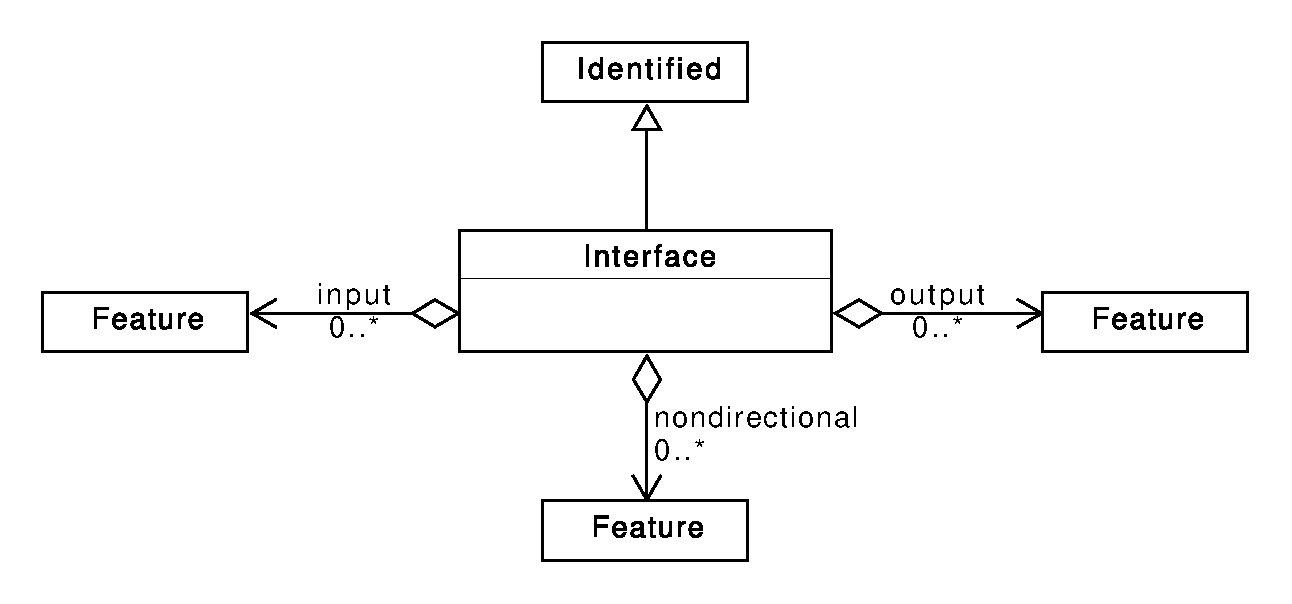
\includegraphics[scale=0.6]{uml/interface}
\caption[]{Diagram of the \sbol{Interface} class and its associated properties.}
\label{uml:interface}
\end{center}
\end{figure}

\subparagraph{The \sbolheading{input} property}
\label{sec:input}

An \sbol{Interface} MAY have any number of \sbol{input} properties, each of type \sbol{IRI}, that MUST reference a \sbol{Feature} object in the same \sbol{Component}.

\subparagraph{The \sbolheading{output} property}
\label{sec:output}

An \sbol{Interface} MAY have any number of \sbol{output} properties, each of type \sbol{IRI}, that MUST reference a \sbol{Feature} object in the same \sbol{Component}.

\subparagraph{The \sbolheading{nondirectional} property}
\label{sec:nondirectional}

An \sbol{Interface} MAY have any number of \sbol{nondirectional} properties, each of type \sbol{IRI}, that MUST reference a \sbol{Feature} object in the same \sbol{Component}. Note that nondirectional can imply both bidirectional as well as situations where there are no flows (for instance -- a physical interface).





\subsection{CombinatorialDerivation}
\label{sec:CombinatorialDerivation}

The purpose of the \sbol{CombinatorialDerivation} class is to specify combinatorial biological designs without having to specify every possible design variant. For example, a \sbol{CombinatorialDerivation} can be used to specify a library of reporter gene variants that include different promoters and RBSs without having to specify a \sbol{Component} for every possible combination of promoter, RBS, and CDS in the library. \sbol{Component} objects that realize a \sbol{CombinatorialDerivation} can be derived in accordance with the class properties \sbol{template}, \\
\sbol{hasVariableFeature}, and \sbol{strategy} (see \ref{uml:combinatorial_derivation}).

\begin{figure}[ht]
\begin{center}
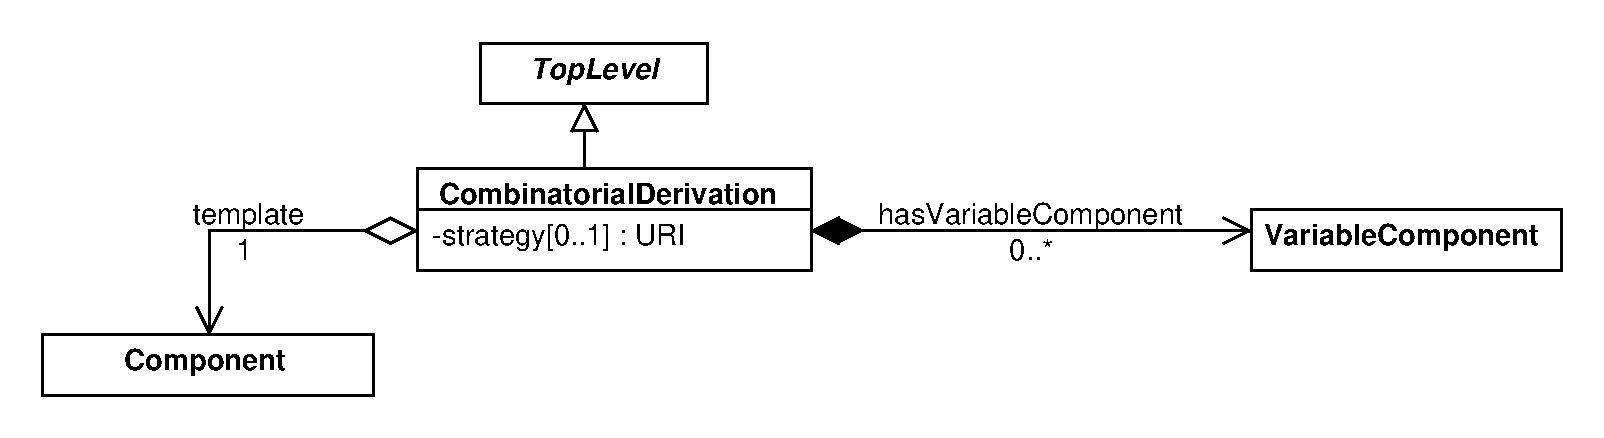
\includegraphics[scale=0.6]{uml/combinatorial_derivation}
\caption[]{Diagram of the \sbol{CombinatorialDerivation} class and its associated properties.}
\label{uml:combinatorial_derivation}
\end{center}
\end{figure}

\subparagraph{The \sbolheading{template} property}\label{sec:template}

The \sbol{template} property is REQUIRED and MUST contain a IRI that refers to a \sbol{Component}. 
This \sbol{Component} is expected to serve as a template for the derivation of new \sbol{Component} objects. 
Consequently, its \sbol{hasFeature} properties SHOULD contain one or more \sbol{Feature} objects that will serve as the variables whose values are set during derivation (referred to hereafter as template \sbol{Feature} objects).
Its other property values describe aspects of the template that will not change based on the values that may be varied.

\subparagraph{The \sbolheading{hasVariableFeature} property}
\label{sec:hasVariableFeature}

Each \sbol{VariableFeature} child of a \sbol{CombinatorialDerivation} defines the set of possible values for one of the variables in the \sbol{template}.
A \sbol{CombinatorialDerivation} object can have zero or more \sbol{hasVariableFeature} properties, each of type \sbol{IRI}, specifying a \sbol{VariableFeature}. 
The set of \sbol{hasVariableFeature} properties MUST NOT contain two or more \sbol{VariableFeature} objects that refer to the same template \\sbol{Feature} via their \sbol{variable} properties (i.e., do not define the same variable twice).

The \sbol{variable} properties of \sbol{VariableFeature} objects determined which \sbol{Feature} objects in the \sbol{template} are modified in a derived \sbol{Component}, and which ones will not be changed.
In particular, we will refer to a \sbol{Feature} in the template \sbol{Component} that is referred to by some \sbol{variable} property as a variable \sbol{Feature}, and one that is not referred to by any as a static \sbol{Feature}.

\subparagraph{The \sbolheading{strategy} property}\label{sec:strategy}
The \sbol{strategy} property is OPTIONAL and has a data type of IRI. \ref{tbl:strategy} provides a list of REQUIRED \sbol{strategy} URLs. If the \sbol{strategy} property is not empty, then it MUST contain a URL from \ref{tbl:strategy}. This property recommends how many \sbol{Component} objects SHOULD be derived from the template \sbol{Component}.

\begin{table}[ht]
  \begin{edtable}{tabular}{lp{4in}}
    \toprule
    \textbf{Strategy URL} & \textbf{Description} \\
    \midrule
    \url{http://sbols.org/v3#enumerate}  &  Derivation SHOULD produce all possible \sbol{Component} objects specified by the \sbol{CombinatorialDerivation}. \\
        \url{http://sbols.org/v3#sample}  & Derivation SHOULD produce a subset of possible \sbol{Component} objects specified by \sbol{CombinatorialDerivation}. The manner in which this subset is chosen is left unspecified. \\
    \bottomrule
  \end{edtable}
  \caption{REQUIRED \sbol{URL}s for the \sbol{strategy} property.}
  \label{tbl:strategy}
\end{table}

\subparagraph{Executing a derivation}

When a \sbol{CombinatorialDerivation} is evaluated to produce a set of derived \sbol{Component} objects, the relationship between the two SHOULD be recorded by means of \prov{wasDerivedFrom} properties. 
In particular:
\begin{itemize}
\item Any derived \sbol{Component} SHOULD have a \prov{wasDerivedFrom} property that refers to the \sbol{CombinatorialDerivation}. 
\item Any \sbol{Feature} in a derived \sbol{Component} SHOULD have a \prov{wasDerivedFrom} property that refers to its corresponding \sbol{Feature} in the template \sbol{Component}.
\item Any \sbol{Collection} produced by the derivation process and containing only derived \sbol{Component} objects SHOULD also have a \prov{wasDerivedFrom} property that refers to the \sbol{CombinatorialDerivation}.
\end{itemize}

All derived objects MUST be consistent with the specification provided in the \sbol{CombinatorialDerivation}.
In particular:
\begin{itemize}
\item Every value of the \sbolmult{type:C}{type} and \sbolmult{role:C}{role} properties of the template \sbol{Component} SHOULD be contained in the values of the corresponding properties in each derived \sbol{Component}.
\item Any static \sbol{Feature} in the template \sbol{Component} SHOULD correspond to a \sbol{Feature} with identical properties in each derived \sbol{Component}.
\item Any variable \sbol{Feature} in the template \sbol{Component} SHOULD be replaced in each derived \sbol{Component} by a number of \sbol{Feature} objects constrained by the number specified by the \sbol{cardinality} property of the \sbol{VariableFeature} (see \ref{tbl:cardinality}).
\item Each property of a \sbol{Feature} object in the derived \sbol{Component} that replaces a variable \sbol{Feature} in the template \sbol{Component} MUST be derived from the values of the associated \sbol{VariableFeature}. 
\item All derived \sbol{Feature} object MUST follow the \sbol{restriction} properties of any \sbol{Constraint} objects that refer to their corresponding template \sbol{Feature}. This will typically be used to rule out illegal combinations of variable values.
\item The \sbolmult{role:F}{role} property of a derived \sbol{Feature} SHOULD contain the same values as the \sbolmult{role:F}{role} property did in the template \sbol{Feature}. 
\item The \sbolmult{type:C}{type} property of a derived \sbol{Feature} or its type-determining referent 
(\sbol{instanceOf} for \sbol{SubComponent}, or that determined for the \sbol{Feature} referred to by a \sbol{ComponentReference})
SHOULD contain the same values as the \sbolmult{type:C}{type} property did in the template \sbol{Feature} or its type-determining referent.
\end{itemize}



\subsubsection{VariableFeature}
\label{sec:VariableFeature}

As described \sbolmult{hasVariableFeature}{above}, the \sbol{VariableFeature} class specifies a variable and set of values that will replace one of the \sbol{Feature} objects in the \sbol{template} of a \sbol{CombinatorialDerivation}.
The variable is specified by the \sbol{variable} property,
and the set of values is defined by the union of \sbol{Component} objects referred to by the \sbol{variant}, \sbol{variantCollection}, and \sbol{variantDerivation} properties.

Note that this union is intended to be a set and not a multi-set.
For example, if the \sbol{variant} property contains a \sbol{Component} $A$ and the \sbol{variantCollection} property has a \sbol{Collection} containing both \sbol{Component} $A$ and  \sbol{Component} $B$, then $A$ SHOULD NOT be selected twice during enumeration, and it SHOULD NOT be selected twice as much as $B$ during sampling.

Given a set of values linked from a \sbol{VariableFeature}, it SHOULD be the case that all value are of type \sbol{om:Measure} or else all values are of type \sbol{Feature}. At present, it is explicitly left undefined how derivation of new components ought to handle mixtures of \sbol{om:Measure} and \sbol{Feature} values.

\begin{figure}[ht]
\begin{center}
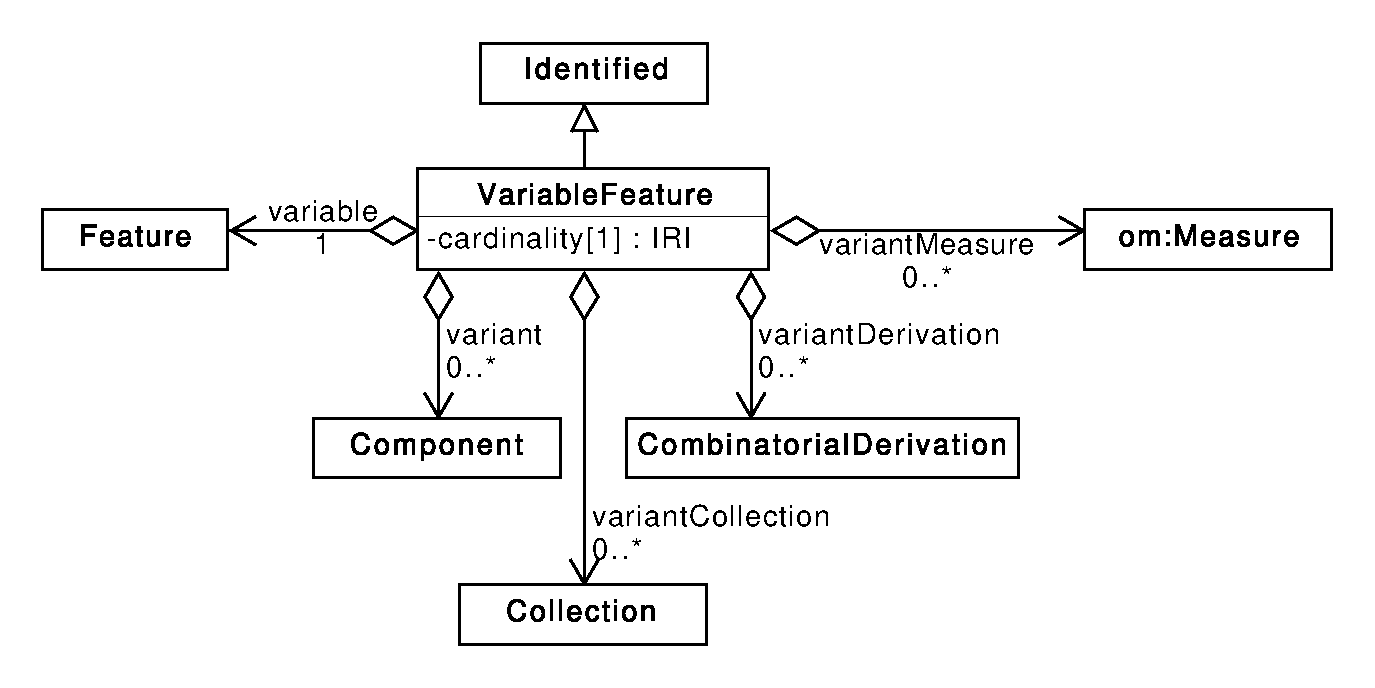
\includegraphics[scale=0.6]{uml/variable_component}
\caption[]{Diagram of the \sbol{VariableFeature} class and its associated properties.}
\label{uml:variable_component}
\end{center}
\end{figure}

\subparagraph{The \sbolheading{variable} property}\label{sec:variable}

The \sbol{variable} property is REQUIRED and MUST contain a IRI that refers to a template \sbol{Feature} in the \sbol{template} \sbol{Component} referred to by this \sbol{VariableFeature}'s parent \sbol{CombinatorialDerivation}

\subparagraph{The \sbolheading{variantMeasure} property}\label{sec:variantMeasure}

A \sbol{VariableFeature} object can have zero or more \sbol{variantMeasure} properties, each of type \sbol{IRI}, specifying a \sbol{om:Measure} object. This property specifies numerical values that are options to be applied to the \sbol{variable} \sbol{Feature} from the \sbol{template} when deriving a new \sbol{Component}.

Note that because a \sbol{om:Measure} is not a \sbol{TopLevel}, the vlaues of \sbol{variantMeasure} must be child objects of the \sbol{VariableFeature}.

\subparagraph{The \sbolheading{variant} property}\label{sec:variant}

A \sbol{VariableFeature} object can have zero or more \sbol{variant} properties, each of type \sbol{IRI}, specifying a \sbol{Component} object. This property specifies individual \sbol{Component} objects to serve as options when deriving a new \sbol{Feature} for the \sbol{variable} \sbol{Feature} from the \sbol{template}.

\subparagraph{The \sbolheading{variantCollection} property}\label{sec:variantCollection}

A \sbol{VariableFeature} object can have zero or more \sbol{variantCollection} properties, each of type \sbol{IRI}, specifying a \sbol{Collection} object.
Such a \sbol{Collection} MUST NOT contain any objects besides \sbol{Component} objects or \sbol{Collection} objects that themselves contain only \sbol{Component} or \sbol{Collection} objects.
This property enables the specification of existing groups of \sbol{Component} objects to serve as options.

\subparagraph{The \sbolheading{variantDerivation} property}\label{sec:variantDerivation}

A \sbol{VariableFeature} object can have zero or more \sbol{variantDerivation} properties, each of type \sbol{IRI}, specifying a \sbol{CombinatorialDerivation} object. 
This property enables the specification of \sbol{Component} objects derived in accordance with another \sbol{CombinatorialDerivation} to serve as options when deriving a new \sbol{Feature} for the \sbol{variable} \sbol{Feature} from the \sbol{template}. 
The \sbol{variantDerivation} properties of a \sbol{VariableFeature} MUST NOT refer to the \sbol{CombinatorialDerivation} that contains this \sbol{VariableFeature}. 
Furthermore, such \sbol{VariableFeature} objects MUST NOT form a cyclical chain of references via their \sbol{variantDerivation} properties and the \sbol{CombinatorialDerivation} objects that contain them. 

\subparagraph{The \sbolheading{cardinality} property}\label{sec:cardinality}

The \sbol{cardinality} property is REQUIRED and has type of IRI. This property specifies how many \sbol{Feature} objects SHOULD be derived from the template \sbol{Feature} during the derivation of a new \sbol{Component}. The value of this property MUST come from the URLs provided in~\ref{tbl:cardinality}.

\begin{table}[ht]
  \begin{edtable}{tabular}{lp{4in}}
    \toprule
    \textbf{Cardinality URL} & \textbf{Description} \\
    \midrule
    \url{http://sbols.org/v3#zeroOrOne} & No more than one \sbol{Feature} in the derived \sbol{Component} SHOULD have a \prov{wasDerivedFrom} property that refers to the template \sbol{Feature}. \\
        \url{http://sbols.org/v3#one} & Exactly one \sbol{Feature} in the derived \sbol{Component} SHOULD have a \prov{wasDerivedFrom} property that refers to the template \sbol{Feature}. \\
\url{http://sbols.org/v3#zeroOrMore} & Any number of \sbol{Feature} objects in the derived \sbol{Component} MAY have \prov{wasDerivedFrom} properties that refer to the template \sbol{Feature}. \\
\url{http://sbols.org/v3#oneOrMore} & At least one \sbol{Feature} in the derived \sbol{Component} SHOULD have a \prov{wasDerivedFrom} property that refers to the template \sbol{Feature}. \\
    \bottomrule
  \end{edtable}
  \caption{REQUIRED \sbol{URL}s for the \sbol{cardinality} property.}
  \label{tbl:cardinality}
\end{table}



\subsection{Implementation}
\label{sec:Implementation}


An \sbol{Implementation} represents a realized instance of a \sbol{Component}, such a sample of DNA resulting from fabricating a genetic design or an aliquot of a specified reagent.
Importantly, an \sbol{Implementation} can be associated with a laboratory sample that was already built, or that is planned to be built in the future. 
An \sbol{Implementation} can also represent virtual and simulated instances.  
An \sbol{Implementation} may be linked back to its original design using the \sbol{prov:wasDerivedFrom} property inherited from the \sbol{Identified} superclass. An \sbol{Implementation} may also link to a \sbol{Component} that specifies its realized structure and/or function.
% as described in Section2.1.1.

\begin{figure}[ht]
\begin{center}
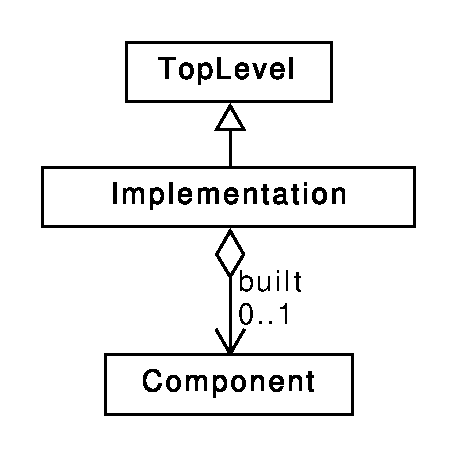
\includegraphics[scale=0.65]{uml/implementation}
\caption[]{Diagram of the \sbol{Implementation} class and its associated properties.}
\label{uml:implementation}
\end{center}
\end{figure}

\subparagraph{The \sbolheading{built} property}\label{sec:built}
The \sbol{built} property is OPTIONAL and MAY contain a URI that MUST refer to a \sbol{Component}. This \sbol{Component} is intended to describe the actual physical structure and/or functional behavior of the \sbol{Implementation}. When the built property refers to a \sbol{Component} that is also linked to the \sbol{Implementation} via PROV-O properties such as \prov{wasDerivedFrom} (see \ref{sec:provenance}), it can be inferred that the actual structure and/or function of the \sbol{Implementation} matches its original design. When the \sbol{built} property refers to a different \sbol{Component}, it can be inferred that the \sbol{Implementation} has deviated from the original design. For example, the latter could be used to document when the DNA sequencing results for an assembled construct do not match the original target sequence.





\subsection{ExperimentalData}
\label{sec:ExperimentalData}


\begin{figure}[ht]
\begin{center}
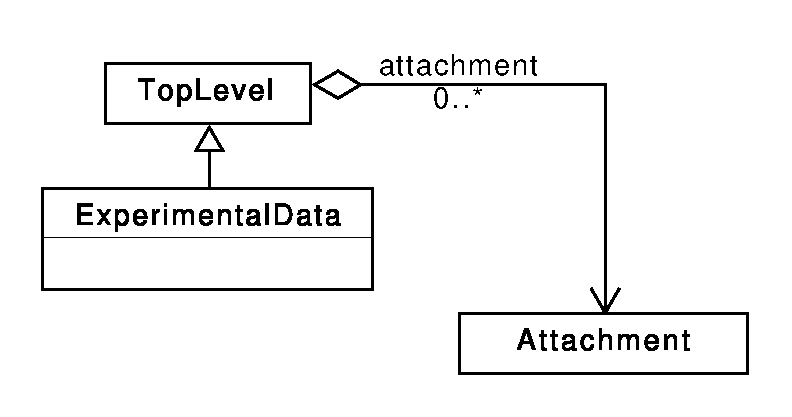
\includegraphics[scale=0.6]{uml/experimental_data}
\caption[]{Diagram of the \sbol{ExperimentalData} class and its associated properties.}
\label{uml:experimental_data}
\end{center}
\end{figure}

The purpose of the \sbol{ExperimentalData} class is to aggregate links to experimental data files. An \sbol{ExperimentalData} is typically associated with a single sample, lab instrument, or experimental condition and can be used to describe the output of the test phase of a design-build-test-learn workflow. For an example of the latter, see \ref{images:design-build-test-learn}.

As shown in \ref{uml:experimental_data}, the \sbol{ExperimentalData} class aggregates links to experimental data files using the OPTIONAL \sbol{hasAttachment} property that it inherits from the \sbol{TopLevel} class.


% -----------------------------------------------------------------------------
\section{SBOL Data Model}\label{sec:model}
% * <nicholas.roehner@gmail.com> 2015-06-03T17:32:14.465Z:
%
%
%
% -----------------------------------------------------------------------------

In this section, we describe the types of biological design data that can belong to an SBOL document and the relationships between these data types. The SBOL data model is specified using Unified Modeling Language (UML) 2.0 diagrams \href{http://www.omg.org/spec/UML/2.0/}{(OMG 2005)}. Subsections \ref{sec:umldiagrams}, \ref{sec:nameconventions}, \ref{sec:datatypes} review the basics of UML diagrams and explain the naming conventions and generic data types used in this specification. The remaining sections then describe the SBOL data model in detail. Complete SBOL examples and best practices when using the standard can be found in \ref{sec:examples} and \ref{sec:bestpractices}, respectively.

\subsection{Understanding the UML Diagrams}
\label{sec:umldiagrams}

The types of biological design data modeled by SBOL are commonly referred to as {\em classes}, especially when discussing the details of software implementation. Each SBOL class can be instantiated by many SBOL objects. These objects MAY contain data that differ in content, but they MUST agree on the type and form of their data as dictated by their common class. Classes are represented in UML diagrams as rectangles labeled at the top with class names.

Classes can be connected to other classes by association properties, which are represented in UML diagrams as arrows. These arrows are labeled with data cardinalities in order to indicate how many values a given association property can possess (see below). The remaining (non-association) properties of a class are listed below its name. Each of the latter properties is labeled with its data type and cardinality.

In the case of an association property, the class from which the arrow originates is the owner of the association property. A diamond at the origin of the arrow indicates the type of association. Open-faced diamonds indicate shared aggregation, in which the owner of the association property exists independently of its value. In the SBOL data model, the value of an association property MUST be a \sbol{URI} or set of \sbol{URI}s that refer to SBOL objects belonging to the class at the tip of the arrow.

By contrast, filled diamonds indicate composite aggregation, also known as a part-whole relationship, in which the value of the association property MUST NOT exist independently of its owner.
In addition, in the SBOL data model, it is REQUIRED that the value of each composite aggregation property is a unique SBOL object (that is, not the value for more than one such property).
Note that in all cases, composite aggregation is used in such a way that there SHOULD NOT be duplication of such objects.

All SBOL properties are labeled with one of several restrictions on data cardinality. These are:

\begin{itemize}

\item $1$ - REQUIRED, one: there MUST be exactly one value for this property.

\item $0 \ldots 1$ - OPTIONAL: there MAY be a single value for this property, or it MAY be absent.

\item $0 \ldots *$ - unbounded: there MAY be any number of values for this property, including none.

\item $1 \ldots *$ - REQUIRED, unbounded: there MAY be any number of values for this property, as long as there is at least one.

\item $n \ldots *$ - at least: there MUST be at least $n$ values for this property.

\end{itemize}

Finally, classes can inherit the properties of other classes. Inheritance relationships are represented in UML diagrams as open-faced, triangular arrows that point from the inheriting class to the inherited class. Some classes in the SBOL data model cannot be instantiated as objects and exist only to group common properties for inheritance. These classes have italicized names and are known as abstract classes.

\subsection{Naming and Font Conventions}
\label{sec:nameconventions}

SBOL classes are named using upper "camel case," meaning that each word is capitalized and all words are run together without spaces, e.g. \sbol{Identified}, \sbol{SequenceAnnotation}.
Properties, on the other hand, are named using lower camel case, meaning that they begin lowercase (e.g., \sbol{identity}) but if they consist of multiple words, all words after the first begin with an uppercase letter (e.g., \sbol{persistentIdentity}).

Within the SBOL data model, each property is given a singular or plural name in accordance with its data cardinalities.
The forms of these names follow the usual rules of English grammar. For example, sequenceAnnotation is the singular form of \sbol{sequenceAnnotations}.

SBOL properties are always given singular names, however, when SBOL objects are serialized (using \emph{Resource Description Framework} (RDF) as described in \ref{sec:serialization}).
This is because the SBOL data model does not contain classes that correspond directly to the RDF elements that group other elements into ordered or unordered sets. Consequently, if an SBOL property has multiple values, then it is serialized as multiple property entries, each with a singular name and a single value.
For example, if an SBOL property has five values, then its serialization contains five RDF triples, each with a singular predicate name and one of the five values as its object.

\subsection{Data Types}
\label{sec:datatypes}
\label{sec:String}
\label{sec:Integer}
\label{sec:Long}
\label{sec:Double}
\label{sec:Boolean}
\label{sec:URI}
\label{sec:literal}

When SBOL use simple ``primitive'' data types such as \sbol{String}s or \sbol{Integer}s, these are defined as the following specific formal types:
\begin{itemize}
\item \sbol{String}: \url{http://www.w3.org/TR/xmlschema11-2/#string}\\
  {\em Example: ``LacI coding sequence''}
\item \sbol{Integer}: \url{http://www.w3.org/TR/xmlschema11-2/#integer}\\
  {\em Example: 3}
\item \twotwozero{\sbol{Long}:} \url{http://www.w3.org/TR/xmlschema11-2/#long}\\
  \twotwozero{{\em Example: 9223372036854775806}}
\item \sbol{Double}: \url{http://www.w3.org/TR/xmlschema11-2/#double}\\
  {\em Example: 3.14159}
\item \sbol{Boolean}: \url{http://www.w3.org/TR/xmlschema11-2/#boolean}\\
  {\em Example: \external{true}}
\end{itemize}
The term \sbol{literal} is used to denote an object that can be any of the four types listed above.
In addition to the simple types listed above, SBOL also uses objects with types \emph{Uniform Resource Identifier} (\sbol{URI}) and \emph{XML Qualified Name} (\sbol{QName}):
\begin{itemize}
\item \sbol{URI}: \url{http://www.w3.org/TR/xmlschema11-2/#anyURI}\\
  {\em Example: \external{http://www.partsregistry.org/Part:BBa\_J23119}}
\item \sbol{QName}: \url{http://www.w3.org/TR/xmlschema11-2/#QName}\\
  {\em Example: \external{myapp:Datasheet}} where  \external{myapp="http://www.myapp.org/"}
\end{itemize}

Note that, in compliance with RDF standards, \sbol{URI}s are generally serialized using an \external{rdf:resource} property, e.g.:
\external{rdf:resource="http://www.partsregistry.org/Part:BBa\_J23119"}

It is important to realize that in RDF, a \sbol{URI} might or might not be a resolvable URL (web address).  A \sbol{URI} is always a globally unique identifier within a structured namespace.  In some cases, that name is also a reference to (or within) a document, and in some cases that document can also be retrieved (e.g., using a web browser).

\subsection{Identified}
\label{sec:Identified}

All SBOL-defined classes are directly or indirectly derived from the \sbol{Identified}  abstract class.
This inheritance means that all SBOL objects are uniquely identified using \sbol{URI}s that uniquely refer to these objects within an SBOL document or at locations on the World Wide Web.

As shown in \ref{uml:identified}, the \sbol{Identified} class includes the following properties: \sbol{identity}, \sbol{persistentIdentity}, \sbol{version}, \twotwozero{\sbol{wasDerivedFroms}}, \sbol{name}, \sbol{description}, and \sbol{annotations}. The latter property is described separately in \ref{sec:Annotations}.

When an SBOL resource reference takes the form of a \sbol{URI}, that \sbol{URI} can either be the value of an \sbol{identity} property or the value of a \sbol{persistentIdentity} property.
If the \sbol{URI} is equal to the value of an \sbol{identity} property, then it is guaranteed to be unique, and it refers to precisely one SBOL object with that \sbol{URI}.
If the \sbol{URI} is equal to the value of a \sbol{persistentIdentity} property, then it MAY refer to multiple SBOL objects that are different ``versions'' of each other. These objects SHOULD be compared to one another to determine which single object the \sbol{URI} resolves to (normally the most recent version - see \ref{sec:version}).
Throughout this document, when a \sbol{URI} is used to refer to an SBOL object, it could fall into either of these cases.

\begin{figure}[ht]
\begin{center}
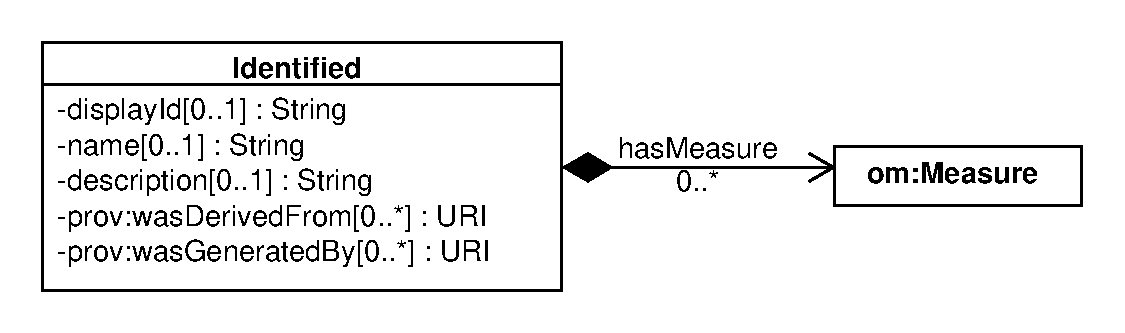
\includegraphics[scale=0.6]{uml/identified}
\caption[]{Diagram of the \sbol{Identified} abstract class and its associated properties}
\label{uml:identified}
\end{center}
\end{figure}

\subsubsection*{The \sbolheading{identity} property}
\label{sec:identity}
The \sbol{identity} property is REQUIRED by all \sbol{Identified} objects and has a data type of \sbol{URI}. A given \sbol{Identified} object's \sbol{identity} \sbol{URI} MUST be globally unique among all other \sbol{identity} \sbol{URI}s. It is also highly RECOMMENDED that the \sbol{URI} structure follows the recommended best practices for compliant \sbol{URI}s specified in \ref{sec:compliant}.

Although most SBOL properties are defined by SBOL and serialized with its namespace, the \sbol{identity} property is defined by the analogous RDF \external{about} property and is serialized with the RDF namespace as follows:

\url{http://www.w3.org/1999/02/22-rdf-syntax-ns\#about}.

The use of \external{about} is expressly for the purpose of making SBOL compliant with pre-existing standards: when you see \external{about} in an SBOL document, you SHOULD interpret it as meaning \sbol{identity}.

\subsubsection*{The \sbolheading{persistentIdentity} property}
\label{sec:persistentIdentity}
The \sbol{persistentIdentity} property is OPTIONAL and has a data type of \sbol{URI}. This \sbol{URI} serves to uniquely refer to a set of SBOL objects \twozeroone{of the same class} that are different versions of each other.

An \sbol{Identified} object MUST be referred to using either its \sbol{identity} \sbol{URI} or its \sbol{persistentIdentity} \sbol{URI}.

\subsubsection*{The \sbolheading{displayId} property}
\label{sec:displayId}
The \sbol{displayId} property is an OPTIONAL identifier with a data type of \sbol{String}. This property is intended to be an intermediate between \sbol{name} and \sbol{identity} that is machine-readable, but more human-readable than the full \sbol{URI} of an \sbol{identity}.

If the \sbol{displayId} property is used, then its \sbol{String} value \twozeroone{\st{SHOULD be locally unique (global uniqueness is not necessary) and}} MUST be composed of only alphanumeric or underscore characters and MUST NOT begin with a digit.

% compliant with the type \external{http://www.w3.org/TR/xmlschema-2/\#NCName}, except that it MUST not include the characters "-" and ".".

\subsubsection*{The \sbolheading{version} property}
\label{sec:version}

The \sbol{version} property is OPTIONAL and has a data type of \sbol{String}. This property can be used to compare two SBOL objects with the same \sbol{persistentIdentity}.

If the \sbol{version} property is used, then it is RECOMMENDED that version numbering follow the conventions of semantic versioning (\url{http://semver.org/}), particularly as implemented by Maven (\url{http://maven.apache.org/}).
This convention represents versions as sequences of numbers and qualifiers that are separated by the characters ``{\tt .}'' and ``{\tt -}'' and are compared in lexicographical order (for example, 1 < 1.3.1 < 2.0-beta).
For a full explanation, see the linked resources.

\subsubsection*{The \sbolheading{wasDerivedFroms} property}
\label{sec:wasDerivedFroms}

\twotwozero{
 The \sbol{wasDerivedFroms} property is OPTIONAL and MAY specify a set of \sbol{URI}s. An SBOL object with this property refers to one or more SBOL objects or non-SBOL resources from which this object was derived.

\twozeroone{The \sbol{wasDerivedFroms} property of a \sbol{TopLevel} SBOL object is subject to the following rules.}
If any members of the \sbol{wasDerivedFroms} property of an SBOL object $A$ that refers to an SBOL object $B$ has an identical \sbol{persistentIdentity}, and both $A$ and $B$ have a \sbol{version}, then the \sbol{version} of $B$ MUST precede that of $A$.
In addition, an SBOL object MUST NOT refer to itself via its own \sbol{wasDerivedFroms} property or form a cyclical chain of references via its \sbol{wasDerivedFroms} property and those of other SBOL objects. For example, the reference chain ``$A$ was derived from $B$ and $B$ was derived from $A$'' is cyclical.
}

\subsubsection*{The \sbolheading{name} property}
\label{sec:name}

The \sbol{name} property is OPTIONAL and has a data type of \sbol{String}. This property is intended to be displayed to a human when visualizing an \sbol{Identified} object.

If an \sbol{Identified} object lacks a name, then software tools SHOULD instead display the object's \sbol{displayId} or \sbol{identity}.
It is RECOMMENDED that software tools give users the ability to switch perspectives between \sbol{name} properties that are human-readable and \sbol{displayId} properties that are less human-readable, but are more likely to be unique.

\subsubsection*{The \sbolheading{description} property}
\label{sec:description}

The \sbol{description} property is OPTIONAL and has a data type of \sbol{String}. This property is intended to contain a more thorough text description of an \sbol{Identified} object.

\subsubsection*{The \sbolheading{annotations} property}
\label{sec:annotations}

The \sbol{annotations} property is OPTIONAL and MAY specify a set of \sbol{Annotation} objects that are contained by the \sbol{Identified} object. The \sbol{Annotation} class is described in more detail in Section~\ref{sec:Annotation}.

\subsubsection*{Serialization}

No complete serialization is defined for \sbol{Identified}, since this
class is only used indirectly through its child classes.  Any such
child class, however, has the following form for serializing
properties inherited from \sbol{Identified}, where CLASS\_NAME is
replaced by the name of the class:

\lstsetsbol
\begin{lstlisting}
<?xml version="1.0" ?>
<rdf:RDF xmlns:pr="http://partsregistry.org" xmlns:rdf="http://www.w3.org/1999/02/22-rdf-syntax-ns#" xmlns:dcterms="http://purl.org/dc/terms/" xmlns:prov="http://www.w3.org/ns/prov#" xmlns:sbol="http://sbols.org/v2#">
  <sbol:CLASS_NAME rdf:about="...">
    [\emph{zero or one}] <sbol:persistentIdentity rdf:resource="..."/> [\emph{element}]
    [\emph{zero or one}] <sbol:displayId>...</sbol:displayId> [\emph{element}]
    [\emph{zero or one}] <sbol:version>...</sbol:version> [\emph{element}]
    [\emph{zero or more}] <prov:wasDerivedFrom rdf:resource="..."/> [\emph{element}]
    [\emph{zero or one}] <dcterms:title>...</dcterms:title> [\emph{element}]
    [\emph{zero or one}] <dcterms:description>...</dcterms:description> [\emph{element}]
               ...
  </sbol:CLASS_NAME>
  ...
</rdf:RDF>
\end{lstlisting}

Note that several of the properties are not in the \external{sbol}
namespace, but are mapped to standardized terms defined elsewhere:
\begin{itemize}
\item \sbol{identity} is serialized as \external{rdf:about}
\item \twotwozero{\sbol{wasDerivedFroms} are} serialized as \external{prov:wasDerivedFrom}
\item \sbol{name} is serialized as \external{dcterms:title}
\item \sbol{description} is serialized as \external{dcterms:description}
\end{itemize}

% \subsection{Documented}
% \label{sec:Documented}
% The \sbol{Documented} abstract class is inherited by the classes of SBOL objects that can contain human-readable properties, such as name and description. This class extends \sbol{Identified} with two additional data properties: \sbol{name}, and \sbol{description} (\ref{uml:documented}).

% \begin{figure}[ht]
% \begin{center}
% \includegraphics[scale=0.6]{uml/documented}
% \caption[]{The \sbol{Documented} abstract class.}
% \label{uml:documented}
% \end{center}
% \end{figure}

% \subsubsection*{Serialization}

% No complete serialization is defined for \sbol{Documented}, since this
% class is only used indirectly through its child classes.  Any such
% child class, however, has the following form for serializing
% properties inherited from \sbol{Documented}, where CLASS\_NAME is
% replaced by the name of the class:

\subsection {TopLevel}
\label{sec:TopLevel}
\sbol{TopLevel} is an abstract class that is extended by any \sbol{Identified} class that can be found at the top level of an SBOL document or file. In other words, \sbol{TopLevel} objects are not nested inside any other object via a composite aggregation or black diamond arrow association property. Instead of nesting, composite \sbol{TopLevel} objects refer to subordinate \sbol{TopLevel} objects by their \sbol{URI}s using shared aggregation or white diamond arrow association properties. The \sbol{TopLevel} classes defined in this specification are \sbol{Sequence}, \sbol{ComponentDefinition}, \sbol{Model}, \sbol{ModuleDefinition},  \sbol{Collection}, \sbol{GenericTopLevel}, \sbol{CombinatorialDerivation}, and \sbol{Implementation}(\ref{uml:toplevel}).

\twotwoone{
\begin{figure}[ht]
\begin{center}
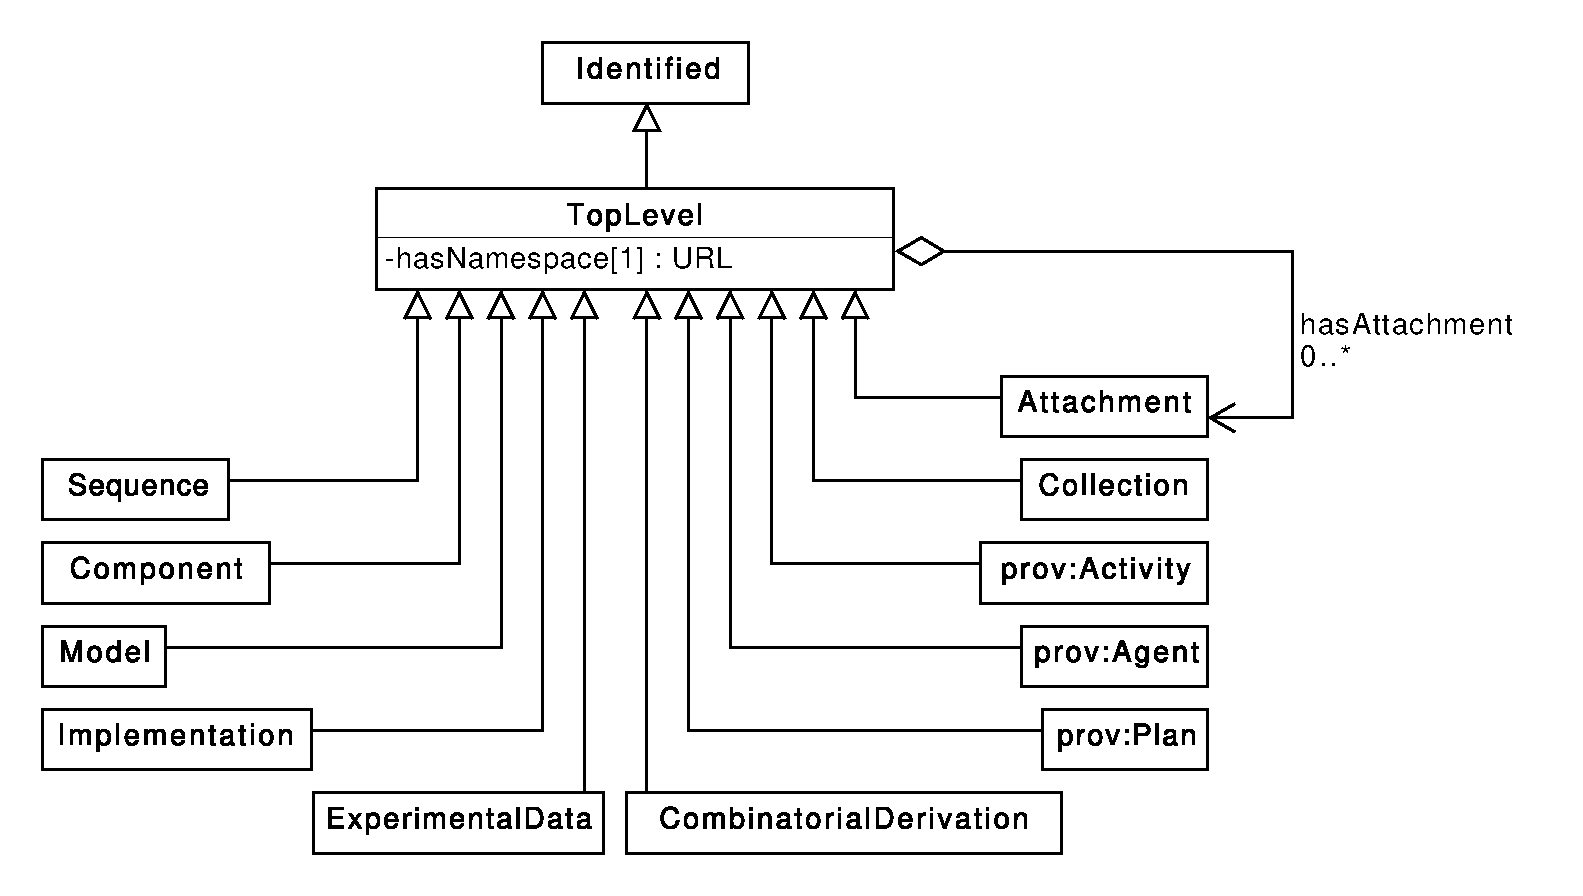
\includegraphics[width=\textwidth]{uml/toplevel}
\caption[]{Classes that inherit from the \sbol{TopLevel} abstract class.}
\label{uml:toplevel}
\end{center}
\end{figure}
}

\subsubsection*{The attachments property}
\label{sec:attachments}
The attachments property is OPTIONAL and MAY specify a set of Attachment objects that are referenced by the TopLevel object. The Attachment class is described in more detail in Section~\ref{sec:Attachment}.

\subsubsection*{Serialization}

No serialization is defined for \sbol{TopLevel}, since this class has no properties of its own and is only used indirectly through its child classes.  All \sbol{TopLevel} classes are serialized one level beneath the RDF document root.


\subsection{Sequence}
\label{sec:Sequence}
The purpose of the \sbol{Sequence} class is to represent the primary structure of a \sbol{ComponentDefinition} object and the manner in which it is encoded. This representation is accomplished  by means of the \sbol{elements} property and \sbol{encoding} property (\ref{uml:sequence}).

\begin{figure}[ht]
\begin{center}
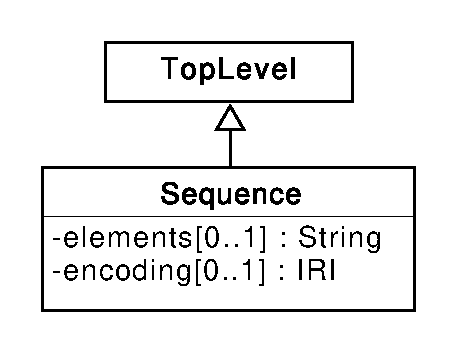
\includegraphics[scale=0.6]{uml/sequence}
\caption[]{Diagram of the \sbol{Sequence} class and its associated properties.}
\label{uml:sequence}
\end{center}
\end{figure}


\subsubsection*{The \sbolheading{elements} property}
\label{sec:elements}
The \sbol{elements} property is a REQUIRED \sbol{String} of characters that represents the constituents of a biological or chemical molecule. For example, these characters could represent the nucleotide bases of a molecule of DNA, the amino acid residues of a protein, or the atoms and chemical bonds of a small molecule.

\subsubsection*{The \sbolheading{encoding} property}
\label{sec:encoding}
The \sbol{encoding} property is REQUIRED and has a data type of \sbol{URI}. This property MUST indicate how the \sbol{elements} property of a \sbol{Sequence} MUST be formed and interpreted.

For example, the \sbol{elements} property of a \sbol{Sequence} with an \external{IUPAC DNA} encoding property MUST contain characters that represent nucleotide bases, such as {\tt a}, {\tt t}, {\tt c}, and {\tt g}. The \sbol{elements} property of a \sbol{Sequence} with a \external{Simplified Molecular-Input Line-Entry System (SMILES)} encoding, on the other hand, MUST contain characters that represent atoms and chemical bonds, such as {\tt C}, {\tt N}, {\tt O}, and {\tt =}.

\ref{tbl:sequence_encodings} provides a list of possible \sbol{URI} values for the \sbol{encoding} property. The terms in \ref{tbl:sequence_encodings} are organized by the type of \sbol{ComponentDefinition} (see \ref{tbl:componentdefinition_types}) that typically refer to a \sbol{Sequence} with such an \sbol{encoding}. \twozeroone{It is RECOMMENDED that the encoding property of a Sequence contains a URI from \ref{tbl:sequence_encodings}.} When the \sbol{encoding} of a \sbol{Sequence} is well described by one of the \sbol{URI}s in \ref{tbl:sequence_encodings}, it MUST contain that \sbol{URI}.

%A Summary of letters for nucleic acids and aminoacids
\begin{table}[ht]
  \begin{edtable}{tabular}{lll}
    \toprule
     \textbf{Encoding} & \textbf{URI} & \textbf{ComponentDefinition Type} \\
    \midrule
     IUPAC DNA, RNA & \url{http://www.chem.qmul.ac.uk/iubmb/misc/naseq.html} & DNA, RNA \\
    IUPAC Protein & \url{http://www.chem.qmul.ac.uk/iupac/AminoAcid/} & Protein\\
   SMILES & \url{http://www.opensmiles.org/opensmiles.html} & SmallMolecule \\
    \bottomrule
  \end{edtable}
  \caption{\sbol{URI}s for specifying the \sbol{encoding} property of a \sbol{Sequence}, organized by the type of \sbol{ComponentDefinition} (see \ref{tbl:componentdefinition_types}) that typically refer to a \sbol{Sequence} with such an \sbol{encoding}.}
  \label{tbl:sequence_encodings}
\end{table}

\subsubsection*{Serialization}
The serialization of a \sbol{Sequence} MUST have the following form:
\lstsetsbol
\begin{lstlisting}
<sbol:Sequence rdf:about="...">
  ... [\emph{properties inherited from identified}] ...
  [\emph{one}] <sbol:elements>...</sbol:elements> [\emph{element}]
  [\emph{one}] <sbol:encoding rdf:resource="..."/> [\emph{element}]
</sbol:Sequence>
\end{lstlisting}

The example below shows the serialization of the \sbol{Sequence} for a promoter. The nucleotide bases of the \sbol{Sequence} are serialized as the \sbol{String} value of its \sbol{elements} property, while its \external{IUPAC DNA} encoding is serialized as the \sbol{URI} value of its  \sbol{encoding} property.

\lstsetsbol
\begin{lstlisting}
<?xml version="1.0" ?>
<rdf:RDF xmlns:rdf="http://www.w3.org/1999/02/22-rdf-syntax-ns#" xmlns:dcterms="http://purl.org/dc/terms/" xmlns:prov="http://www.w3.org/ns/prov#" xmlns:sbol="http://sbols.org/v2#">
  <sbol:Sequence rdf:about="http://partsregistry.org/seq/BBa_J23119">
    <sbol:persistentIdentity rdf:resource="http://partsregistry.org/seq/BBa_J23119"/>
    <sbol:displayId>BBa_J23119</sbol:displayId>
    <prov:wasDerivedFrom rdf:resource="http://parts.igem.org/Part:BBa_J23119:Design"/>
    <sbol:elements>ttgacagctagctcagtcctaggtataatgctagc</sbol:elements>
    <sbol:encoding rdf:resource="http://www.chem.qmul.ac.uk/iubmb/misc/naseq.html"/>
  </sbol:Sequence>
</rdf:RDF>
\end{lstlisting}


\subsection{ComponentDefinition}
\label{sec:ComponentDefinition}

The \sbol{ComponentDefinition} class represents the structural entities of a biological design. The primary usage of this class is to represent structural entities with designed sequences, such as DNA, RNA, and proteins, but it can also be used to represent any other entity that is part of a design, such as small molecules, molecular complexes, and light.

As shown in \ref{uml:component_definition}, the \sbol{ComponentDefinition} class describes a structural design entity using the following properties: \sbolmult{types:CD}{types}, \sbolmult{roles:CD}{roles}, and \sbol{sequences}. In addition, this class has properties for describing and organizing the substructure of said design entity, including \sbol{components}, \sbol{sequenceAnnotations}, and \sbol{sequenceConstraints}.

\begin{figure}[ht]
\begin{center}
\includegraphics[width=0.95\textwidth]{uml/component_definition}
\caption[]{Diagram of the \sbol{ComponentDefinition} class and its associated properties.}
\label{uml:component_definition}
\end{center}
\end{figure}

\subsubsection*{The \sbolheading{types} property}
\label{sec:types:CD}

The \sbolmult{types:CD}{types} property is a REQUIRED set of \sbol{URI}s that
specifies the category of biochemical or physical entity (for example DNA,
protein, or small molecule) that a \sbol{ComponentDefinition} object abstracts
for the purpose of engineering design. For DNA or RNA entities,
additional \sbolmult{types:CD}{types} fields are used to describe nucleic acid
topology (circular / linear) and strandedness (double- or single-stranded).

The \sbolmult{types:CD}{types} property of every \sbol{ComponentDefinition} MUST contain one or more \sbol{URI}s that MUST identify terms from appropriate ontologies, such as the Biological Pathway Exchange (BioPAX) ontology ~\cite{biopax} or  the ontology of Chemical Entities of Biological Interest (ChEBI) ~\cite{chebi}.
\ref{tbl:componentdefinition_types} provides a list of possible ontology terms for the \sbolmult{types:CD}{types} property and their \sbol{URI}s.
In order to maximize the compatibility of designs, \twozeroone{the \sbolmult{types:CD}{types} property of a \sbol{ComponentDefinition} SHOULD contain a \sbol{URI} from \ref{tbl:componentdefinition_types}, and} any \sbol{ComponentDefinition} that can be well-described by one of the terms in \ref{tbl:componentdefinition_types} MUST use the \sbol{URI} for that term as one of its \sbolmult{types:CD}{types}.
Finally, if the \sbolmult{types:CD}{types} property contains multiple \sbol{URI}s, then they MUST identify non-conflicting terms (otherwise, it might not be clear how to interpret them). For example, the BioPAX terms provided by \ref{tbl:componentdefinition_types} would conflict because they specify classes of biochemical entities with different molecular structures.

\begin{table}[ht]
  \begin{edtable}{tabular}{ll}
    \toprule
    \textbf{ComponentDefinition Type} & \textbf{URI for BioPAX Term} \\
    \midrule
    DNA  & \url{http://www.biopax.org/release/biopax-level3.owl#DnaRegion}\\
    RNA  & \url{http://www.biopax.org/release/biopax-level3.owl#RnaRegion}\\
    Protein  & \url{http://www.biopax.org/release/biopax-level3.owl#Protein}\\
    Small Molecule  & \url{http://www.biopax.org/release/biopax-level3.owl#SmallMolecule}\\
    Complex  & \url{http://www.biopax.org/release/biopax-level3.owl#Complex}\\
    \bottomrule
  \end{edtable}
  \caption{BioPAX terms to specify the molecule type using the \sbolmult{types:CD}{types} property of a \sbol{ComponentDefinition}.}
 \label{tbl:componentdefinition_types}
\end{table}

\twoonezero{\emph{Nucleic Acid Topology types}\\
%\vspace{-7pt}
\-\hspace{0.8cm}
[New in 2.1.0; see SEP 011: \url{https://github.com/SynBioDex/SEPs/blob/master/sep_011.md}]

Any \sbol{ComponentDefinition} classified as DNA (see \ref{tbl:componentdefinition_types}) is RECOMMENDED to encode circular/linear topology information in an additional type field. This
(topology) type field SHOULD specify a URI from the Topology Attribute branch of the SO
(this is currently just 'linear' or 'circular' as given in \ref{tbl:componentdefinition_topology}). Topology information SHOULD be specified for DNA \sbol{ComponentDefinition} records with a fully specified sequence, except in three scenarios: if the DNA record doesn't have sequence information, or if the DNA record has incomplete sequence information, or if topology is genuinely unknown. For any \sbol{ComponentDefinition} classified as RNA (see \ref{tbl:componentdefinition_types}), a topology type field is OPTIONAL. The default
assumption in this case is linear topology.  In any case, no more than one topology should be specified.

Any \sbol{ComponentDefinition} classified as DNA or RNA MAY also have strand
information encoded in an additional (third) type field using a URI from the Strand Attribute branch of the SO (currently there are only two possible terms for single or double-stranded nucleic
acids given in \ref{tbl:componentdefinition_topology}). In absence of this field, the
default strand information assumed for DNA is 'double-stranded' and for RNA is
'single-stranded'.

Any other type of \sbol{ComponentDefinition} record (protein, small molecule, etc) SHOULD NOT
have any type field pointing to SO terms from the topology or strand attribute branches of SO.

Note that a \emph{circular} topology instructs software to interpret the
beginning / end position of a given sequence (be it DNA or RNA) as arbitrary so
that sequence features may be mapped or identified across this junction. \emph{Double stranded} instructs software to apply sequence searches to both strands (i.e. sequence and reverse complement of sequence).

\begin{table}[ht]
  \begin{edtable}{tabular}{ll}
    \toprule
    \textbf{Nucleic Acid Topology} & \textbf{URI for Nucleic Acid Topology
      Term in SO} \\
    \midrule
    linear  & \url{http://identifiers.org/so/SO:0000987}\\
    circular  & \url{http://identifiers.org/so/SO:0000988}\\
    single-stranded & \url{http://identifiers.org/so/SO:0000984}\\
    double-stranded & \url{http://identifiers.org/so/SO:0000985}\\
    \bottomrule
  \end{edtable}
  \caption{Sequence Ontology terms to encode DNA or RNA topology information in the \sbolmult{types:CD}{types} properties of a \sbol{ComponentDefinition}.}
 \label{tbl:componentdefinition_topology}
\end{table}
}

\subsubsection*{The \sbolheading{roles} property}
\label{sec:roles:CD}

The \sbolmult{roles:CD}{roles} property is an OPTIONAL set of \sbol{URI}s that clarifies the potential function of the entity represented by a \sbol{ComponentDefinition} in a biochemical or physical context.

The \sbolmult{roles:CD}{roles} property of a \sbol{ComponentDefinition} MAY contain one or more \sbol{URI}s that MUST identify terms from ontologies that are consistent with the \sbolmult{types:CD}{types} property of the \sbol{ComponentDefinition}.
For example, the \sbolmult{roles:CD}{roles} property of a DNA or RNA \sbol{ComponentDefinition} could contain URIs identifying terms from the Sequence Ontology (SO). \twozeroone{As a best practice, a DNA or RNA \sbol{ComponentDefinition} SHOULD contain exactly one \sbol{URI} that refers to a term from the sequence feature branch of the SO.}
\twotwoone{Similarly, the roles property of a Protein and SmallMolecule \sbol{ComponentDefinition} SHOULD respectively contain \sbol{URI}s identifying terms from the \texttt{MolecularFunction} branch (\texttt{GO:0003674}) of the Gene Ontology (GO) and the \texttt{role} branch (\texttt{CHEBI:50906}) of the CHEBI ontology.}
\ref{tbl:componentdefinition_roles} contains a list of possible ontology terms for the \sbolmult{roles:CD}{roles} property and their \sbol{URI}s. These terms are organized by the type of \sbol{ComponentDefinition} to which they SHOULD apply (see \ref{tbl:componentdefinition_types}). Any \sbol{ComponentDefinition} that can be well-described by one of the terms in \ref{tbl:componentdefinition_roles} MUST use the \sbol{URI} for that term as one of its \sbolmult{roles:CD}{roles}.


\begin{table}[ht]
  \begin{edtable}{tabular}{lll}
    \toprule
    \textbf{ComponentDefinition Role} & \textbf{URI for Ontology Term} & \textbf{ComponentDefinition Type} \\
    \midrule
   Promoter & \url{http://identifiers.org/so/SO:0000167} & DNA \\
   RBS & \url{http://identifiers.org/so/SO:0000139} & DNA \\
      CDS & \url{http://identifiers.org/so/SO:0000316} & DNA \\
      Terminator & \url{http://identifiers.org/so/SO:0000141} & DNA \\
      Gene & \url{http://identifiers.org/so/SO:0000704} & DNA \\
      Operator & \url{http://identifiers.org/so/SO:0000057} & DNA \\
      Engineered Gene & \url{http://identifiers.org/so/SO:0000280} & DNA \\
      mRNA & \url{http://identifiers.org/so/SO:0000234} & RNA \\
      Effector & \url{http://identifiers.org/chebi/CHEBI:35224} & Small Molecule \\
      Transcription Factor & \url{http://identifiers.org/go/GO:0003700} & Protein\\
    \bottomrule
  \end{edtable}
  \caption{Ontology terms to specify the \sbolmult{roles:CD}{roles} property of a \sbol{ComponentDefinition}, organized by the type of \sbol{ComponentDefinition} to which they are intended to apply (see \ref{tbl:componentdefinition_types}).}
  \label{tbl:componentdefinition_roles}
\end{table}

\subsubsection*{The \sbolheading{sequences} property}
\label{sec:sequences}
The \sbol{sequences} property is OPTIONAL and MAY include a set of \sbol{URI}s that refer to \sbol{Sequence} objects. These objects define the primary structure of the \sbol{ComponentDefinition}.

Many \sbol{ComponentDefinition} objects will refer to precisely one \sbol{Sequence} object.
For certain use cases, however, it can be appropriate to refer to multiple \sbol{Sequence} objects.
For example, a user might wish to provide two different representations of the structure of a DNA \sbol{ComponentDefinition}, one that represents its structure at the level of nucleotide bases and one that represents its structure at the level of atoms and bonds.

If a \sbol{ComponentDefinition} refers to more than one \sbol{Sequence} object, then these objects MUST be consistent with each other, such that well-defined mappings exist between their \sbol{elements} properties in accordance with their \sbol{encoding} properties. Furthermore, these objects MUST NOT have conflicting \sbol{encoding} properties. For example, the \external{IUPAC} \sbol{encoding} properties provided by \ref{tbl:sequence_encodings} conflict with each other because they do not specify how to encode the same class of biochemical entity. The \external{SMILES} \sbol{encoding}, however, does not conflict with them because it specifies how to encode biochemical entities in general, which includes DNA, RNA, and proteins. If a \sbol{ComponentDefinition} refers to more than one \sbol{Sequence} with the same \sbol{encoding}, then the \sbol{elements} of these \sbol{Sequence} objects SHOULD have equal lengths. These requirements and best practices are intended to make it easier for software tools to locate any regions specified by the \sbol{SequenceAnnotation} objects of a \sbol{ComponentDefinition} on its associated \sbol{Sequence} objects, as well as validate whether its \sbol{Sequence} objects are consistent with those associated with any \sbol{ComponentDefinition} objects that it composes via its \sbol{Component} objects.

Finally, if a \sbol{ComponentDefinition} refers to one or more \sbol{Sequence} objects and its \sbolmult{types:CD}{types} property refers to a term from \ref{tbl:componentdefinition_types}, then one of these \sbol{Sequence} objects MUST have the \sbol{encoding} that is cross-listed with this term in \ref{tbl:sequence_encodings}.
Conversely, if a \sbol{ComponentDefinition} refers to a \sbol{Sequence} with an \sbol{encoding} from \ref{tbl:sequence_encodings}, then its \sbolmult{types:CD}{types} property MUST refer to the term from \ref{tbl:componentdefinition_types} that is cross-listed with this \sbol{encoding} in \ref{tbl:sequence_encodings}.
For example, if the \sbolmult{types:CD}{types} property of a \sbol{ComponentDefinition} refers to the BioPAX term for DNA, then one of the \sbol{Sequence} objects to which it refers (if any) MUST have an \external{IUPAC DNA} \sbol{encoding}, and if a \sbol{ComponentDefinition} refers to a \sbol{Sequence} with an \external{IUPAC DNA} \sbol{encoding}, then its \sbolmult{types:CD}{types} property MUST refer to the BioPAX term for DNA. These requirements are meant to provide for some degree of consistency between the \sbolmult{types:CD}{types} property of a \sbol{ComponentDefinition} and the \sbol{encoding} properties of the \sbol{Sequence} objects to which the \sbol{ComponentDefinition} refers.

\subsubsection*{The \sbolheading{components} property}
\label{sec:components}

The \sbol{components} property is OPTIONAL and MAY specify a set of \sbol{Component} objects that are contained by the \sbol{ComponentDefinition}. The set of relations between \sbol{Component} and \sbol{ComponentDefinition} objects is strictly acyclic (see \ref{sec:ComponentInstance}).

While the \sbol{ComponentDefinition} class is analogous to a blueprint or specification sheet for a biological part, the \sbol{Component} class represents the specific occurrence of a part within a design.
Hence, this class allows a biological design to include multiple instances of a particular part (defined by reference to the same \sbol{ComponentDefinition}). For example, the \sbol{ComponentDefinition} of a polycistronic gene could contain two \sbol{Component} objects that refer to the same \sbol{ComponentDefinition} of a CDS.

The \sbol{components} properties of \sbol{ComponentDefinition} objects can be used to construct a hierarchy of \sbol{Component} and \sbol{ComponentDefinition} objects. If a \sbol{ComponentDefinition} in such a hierarchy refers to one or more \sbol{Sequence} objects, and there exist \sbol{ComponentDefinition} objects lower in the hierarchy that refer to \sbol{Sequence} objects with the same \sbol{encoding}, then the \sbol{elements} properties of these \sbol{Sequence} objects SHOULD be consistent with each other, such that well-defined mappings exist from the ``lower level'' \sbol{elements} to the ``higher level'' \sbol{elements} in accordance with their shared \sbol{encoding} properties. This mapping is also subject to any restrictions on the positions of the \sbol{Component} objects in the hierarchy that are imposed by the \sbol{SequenceAnnotation} or \sbol{SequenceConstraint} objects contained by the \sbol{ComponentDefinition} objects in the hierarchy.

A DNA \sbol{ComponentDefinition}, for example, could refer to a \sbol{Sequence} with an \external{IUPAC DNA} \sbol{encoding} and an \sbol{elements} \external{String} of ``{\tt gattaca}.'' In turn, this \sbol{ComponentDefinition} could contain a \sbol{Component} that refers to a ``lower level''  \sbol{ComponentDefinition} that also refers to a \sbol{Sequence} with an \external{IUPAC DNA} \sbol{encoding}. Consequently, a consistent \sbol{elements} \external{String} of this ``lower level'' \sbol{Sequence} could be ``{\tt gatta},'' or perhaps ``{\tt tgta}'' if the \sbol{Component} is positioned by a \sbol{SequenceAnnotation} that contains a \sbol{Location}  with an \sbol{orientation} of ``reverse complement'' (see \ref{sec:Location}).

% If the \sbol{ComponentDefinition} refers to a \sbol{Sequence} with an \external{IUPAC} \sbol{encoding} from \ref{tbl:sequence_encodings}, then each \sbol{Component} in its \sbol{components} property MUST refer to a \sbol{ComponentDefinition} that refers to a \sbol{Sequence} with the same \sbol{encoding}.
% In addition, it MUST be possible to align the \sbol{elements} of the latter \sbol{Sequence} objects to the \sbol{elements} of the \sbol{ComponentDefinition}'s \sbol{Sequence}, subject to any restrictions imposed by the \sbol{SequenceAnnotation} and \sbol{SequenceConstraint} objects that refer to the contents of the \sbol{components} property.
% A DNA \sbol{ComponentDefinition}, for example, could refer to a \sbol{Sequence} that has an \external{IUPAC DNA} \sbol{encoding} and an \sbol{elements} \external{String} of ``{\tt gattaca}.'' In this case, any \sbol{Component} contained by this \sbol{ComponentDefinition} would itself need to have a \sbol{ComponentDefinition} that refers to a \sbol{Sequence} that has an \external{IUPAC DNA} \sbol{encoding} and an \sbol{elements} \external{String} that can be aligned with ``{\tt gattaca},'' such as ``{\tt gatta}," or perhaps ``{\tt tgta}'' in the case of a \sbol{Component} that is positioned by a \sbol{SequenceAnnotation} with a \sbol{Location} \sbol{orientation} of ``reverse complement'' (see \ref{sec:Location}).

% Furthermore, this \sbol{Sequence} MUST have the same \external{IUPAC} \sbol{encoding} as a \sbol{Sequence} of the parent \sbol{ComponentDefinition} that contains the \sbol{SequenceAnnotation}.

\subsubsection*{The \sbolheading{sequenceAnnotations} property}
\label{sec:sequenceAnnotations}

The \sbol{sequenceAnnotations} property is OPTIONAL and MAY contain a set of \sbol{SequenceAnnotation} objects. Each \sbol{SequenceAnnotation} specifies and describes a potentially discontiguous region on the \sbol{Sequence} objects referred to by the \sbol{ComponentDefinition}.

In addition, each \sbol{SequenceAnnotation} can  position a \sbol{Component} of the \sbol{ComponentDefinition} at the region specified by its \sbol{Location} objects (see \ref{sec:Location}). The \sbol{sequenceAnnotations} property MUST NOT contain two or more \sbol{SequenceAnnotation} objects that refer to the same \sbol{Component} in this way.

Finally, as a best practice, if a \sbol{ComponentDefinition} refers to a \sbol{Sequence} with an \external{IUPAC} \sbol{encoding} from \ref{tbl:sequence_encodings}, then each of its \sbol{SequenceAnnotation} objects that contains a \sbol{Range} or \sbol{Cut} SHOULD specify a region on the \sbol{elements} of this \sbol{Sequence}.
For example, the \sbol{ComponentDefinition} of a eukaryotic gene could refer to a \sbol{Sequence} with an \external{IUPAC DNA} \sbol{encoding}. In order to specify the discontiguous region occupied by its CDS, this gene \sbol{ComponentDefinition} would need a \sbol{SequenceAnnotation} that contains one or more \sbol{Range} objects, each one specifying \sbol{start} and \sbol{end} positions that correspond to indices of the \sbol{elements} of its DNA \sbol{Sequence}.

\subsubsection*{The \sbolheading{sequenceConstraints} property}
\label{sec:sequenceConstraints}

The \sbol{sequenceConstraints} property is OPTIONAL and MAY contain a set of \sbol{SequenceConstraint} objects. These objects describe any restrictions on the relative, sequence-based positions and/or orientations of the \sbol{Component} objects contained by the \sbol{ComponentDefinition}.
For example, the \sbol{ComponentDefinition} of a gene might specify that the position of its promoter \sbol{Component} precedes that of its CDS \sbol{Component}. This is particularly useful when a \sbol{ComponentDefinition} lacks a \sbol{Sequence} and therefore cannot specify the precise, sequence-based positions of its \sbol{Component} objects using \sbol{SequenceAnnotation} objects.

\subsubsection*{Serialization}
The serialization of a \sbol{ComponentDefinition} MUST have the form below.
The \sbol{components},  \sbol{sequenceConstraints},  \sbol{sequenceAnnotations}, and \sbol{sequences} properties of a \sbol{ComponentDefinition} contain or reference objects belonging to the appropriate SBOL classes as their values, while the \sbolmult{types:CD}{types} and \sbolmult{roles:CD}{roles} properties contain \sbol{URI}s that identify ontology terms as their values.

As shown below, each of these objects and \sbol{URI}s are serialized as part of an implicit set of SBOL properties with singular rather then plural names.
In particular, each object is serialized as an RDF/XML node nested within a property, while each \sbol{URI} (except the \sbol{identity}) is serialized as an \external{rdf:resource} on a property.

\lstsetsbol
\begin{lstlisting}
<sbol:ComponentDefinition rdf:about="...">
  ... [\emph{properties inherited from identified}] ...
  [\emph{zero or more}]  <sbol:sequence rdf:resource="..."/> [\emph{element}]
  [\emph{one or more}]   <sbol:type rdf:resource="..."/> [\emph{elements}]
  [\emph{zero or more}]  <sbol:role rdf:resource="..."/> [\emph{elements}]
  [\emph{zero or more}]  <sbol:component>
                 <sbol:Component rdf:about="...">...</sbol:Component>
               </sbol:component> [\emph{elements}]
  [\emph{zero or more}] <sbol:sequenceAnnotation>
                 <sbol:SequenceAnnotation rdf:about="...">...</sbol:SequenceAnnotation>
               </sbol:sequenceAnnotation> [\emph{elements}]
  [\emph{zero or more}] <sbol:sequenceConstraint>
                 <sbol:SequenceConstraint rdf:about="...">...</sbol:SequenceConstraint>
               </sbol:sequenceConstraint> [\emph{elements}]
</sbol:ComponentDefinition>
\end{lstlisting}


The example below shows the serialization for the \sbol{ComponentDefinition} of a promoter. The BioPAX term \external{DnaRegion} and the ChEBI term \external{CHEBI:4705} (\external{double-stranded DNA}) are used to indicate that the type of biological entity represented by this \sbol{ComponentDefinition} is DNA. Its role is specified using the SO terms \external{SO:0000167} (\external{promoter}) and the more specific \external{SO:0000613} (\external{bacterial\_RNApol\_promoter}).

\lstsetsbol
\begin{lstlisting}
<?xml version="1.0" ?>
<rdf:RDF xmlns:rdf="http://www.w3.org/1999/02/22-rdf-syntax-ns#" xmlns:dcterms="http://purl.org/dc/terms/" xmlns:prov="http://www.w3.org/ns/prov#" xmlns:sbol="http://sbols.org/v2#">
  <sbol:ComponentDefinition rdf:about="http://partsregistry.org/cd/BBa_J23119">
    <sbol:persistentIdentity rdf:resource="http://partsregistry.org/cd/BBa_J23119"/>
    <sbol:displayId>BBa_J23119</sbol:displayId>
    <prov:wasDerivedFrom rdf:resource="http://partsregistry.org/Part:BBa_J23119"/>
    <dcterms:title>J23119 promoter</dcterms:title>
    <dcterms:description>Constitutive promoter</dcterms:description>
    <sbol:type rdf:resource="http://www.biopax.org/release/biopax-level3.owl#DnaRegion"/>
    <sbol:type rdf:resource="http://identifiers.org/so/SO:0000987">
    <sbol:role rdf:resource="http://identifiers.org/so/SO:0000167"/>
    <sbol:role rdf:resource="http://identifiers.org/so/SO:0000613"/>
    <sbol:sequence rdf:resource="http://partsregistry.org/seq/BBa_J23119"/>
  </sbol:ComponentDefinition>
</rdf:RDF>
\end{lstlisting}


\subsubsection{ComponentInstance}
\label{sec:ComponentInstance}

\begin{figure}[ht]
\begin{center}
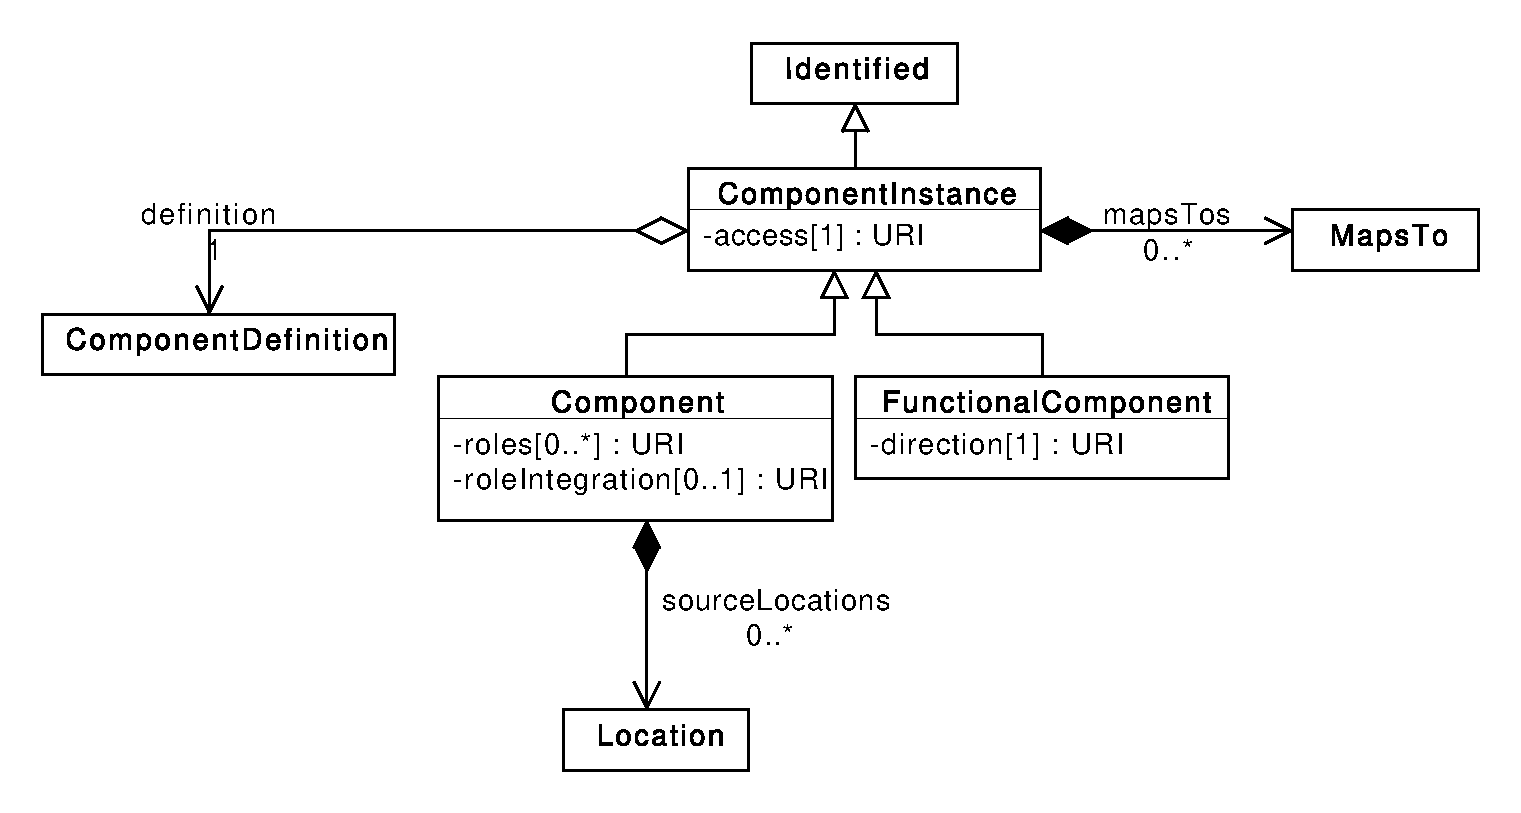
\includegraphics[scale=0.6]{uml/component_instance}
\caption[]{Diagram of the \sbol{ComponentInstance} class and its associated properties.}
\label{uml:component}
\end{center}
\end{figure}

The \sbol{ComponentInstance} abstract class is inherited by SBOL classes that represent the usage or occurrence of a \sbol{ComponentDefinition} within a larger design (that is, another \sbol{ComponentDefinition} or \sbol{ModuleDefinition}). Currently, there are two subclasses of \sbol{ComponentInstance}:
\begin{itemize}
\item The \sbol{Component} class is used to specify the structural usage of a \sbol{ComponentDefinition} inside another \sbol{ComponentDefinition} via the \sbol{components} property.
\item The \sbol{FunctionalComponent} class is used to specify the functional usage of a \sbol{ComponentDefinition} inside a \sbol{ModuleDefinition} via the \sbol{functionalComponents} property. This class is described in \ref{sec:FunctionalComponent}.
\end{itemize}

\paragraph{The \sbolheading{definition} property}
\label{sec:definition:CI}

The \sbolmult{definition:CI}{definition} property is a REQUIRED \sbol{URI} that refers to the \sbol{ComponentDefinition} of the \sbol{ComponentInstance}.
As described in the previous section, this \sbol{ComponentDefinition} effectively provides information about the \sbolmult{types:CD}{types} and \sbolmult{roles:CD}{roles} of the \sbol{ComponentInstance}.

The \sbolmult{definition:CI}{definition} property MUST NOT refer to the same \sbol{ComponentDefinition} as the one that contains the \sbol{ComponentInstance}.
Furthermore, \sbol{ComponentInstance} objects MUST NOT form a cyclical chain of references via their \sbolmult{definition:CI}{definition} properties and the \sbol{ComponentDefinition} objects that contain them.
For example, consider the \sbol{ComponentInstance} objects $A$ and $B$ and the \sbol{ComponentDefinition} objects $X$ and $Y$. The reference chain ``$X$ contains $A$, $A$ is defined by $Y$, $Y$ contains $B$, and $B$ is defined by $X$'' is cyclical.

\paragraph{The \sbolheading{mapsTos} property}\label{sec:mapsTos:CI}

The \sbolmult{mapsTos:CI}{mapsTos} property is OPTIONAL and MAY contain a set of \sbol{MapsTo} objects that refer to and link together \sbol{ComponentInstance} objects (both \sbol{Component} objects and \sbol{FunctionalComponent} objects) within a larger design.

\ref{sec:MapsTo} contains a more detailed description of the \sbol{MapsTo} class.

\paragraph{The \sbolheading{access} property}
\label{sec:access}
\label{sec:public}
\label{sec:private}

The \sbol{access} property is a REQUIRED \sbol{URI} that indicates whether the \sbol{ComponentInstance}
can be referred to remotely by a \sbol{MapsTo} on another \sbol{ComponentInstance} or \sbol{Module} contained by a different parent \sbol{ComponentDefinition} or \sbol{ModuleDefinition} (one that does not contain this \sbol{ComponentInstance}).

\ref{tbl:componentInstance_access} provides a list of REQUIRED \sbol{access} \sbol{URI}s. The value of the \sbol{access} property MUST be one of these \sbol{URI}s.

\begin{table}[ht]
  \begin{edtable}{tabular}{lp{4in}}
    \toprule
    \textbf{Access URI} & \textbf{Description} \\
    \midrule
    \url{http://sbols.org/v2#public}  & The \sbol{ComponentInstance} MAY be referred to by remote \sbol{MapsTo} objects. \\
        \url{http://sbols.org/v2#private}  & The \sbol{ComponentInstance} MUST NOT be referred to by remote \sbol{MapsTo} objects. \\
    \bottomrule
  \end{edtable}
  \caption{REQUIRED \sbol{URI}s for the \sbol{access} property.}
  \label{tbl:componentInstance_access}
\end{table}

In some cases, a designer might want to set the \sbol{access} property of a \sbol{ComponentInstance} such that others cannot map to the \sbol{ComponentInstance} when they reuse its parent \sbol{ComponentDefinition}. For example, a designer who is concerned about retroactivity might set the \sbol{access} of the \sbol{ComponentInstance} to ``private'' in order to prevent its mapping to another \sbol{ComponentInstance} that participates in a new \sbol{Interaction} as part of a composite design.

\paragraph{Serialization}

No serialization is defined for the \sbol{ComponentInstance} class, since this class is only used indirectly through the \sbol{Component} and \sbol{FunctionalComponent} subclasses.

\subsubsection{Component}
\label{sec:Component}
The \sbol{Component} class is used to compose \sbol{ComponentDefinition} objects into a structural hierarchy. For example, the \sbol{ComponentDefinition} of a gene could contain four \sbol{Component} objects: a promoter, RBS, CDS, and terminator. In turn, the \sbol{ComponentDefinition} of the promoter \sbol{Component} could contain \sbol{Component} objects defined as various operator sites.

% All \sbol{Component} objects directly referenced within a \sbol{ComponentDefinition}'s \sbol{SequenceAnnotation} or \sbol{SequenceConstraint} parts MUST be associated with that \sbol{ComponentDefinition} by means of its \sbol{components} property.

\twoonezero{

\paragraph{The \sbolheading{roles} property}\label{sec:roles:C}
\vspace{-7pt}
\-\hspace{0.8cm}[New in 2.1.0; see SEP 004: \url{https://github.com/SynBioDex/SEPs/blob/master/sep_004.md}]

The expected purpose and function of a genetic part are described by the
\sbolmult{roles:CD}{roles} property of \sbol{ComponentDefinition}. However, the same building block might be used for a different purpose in an actual design. In other words, purpose and function are sometimes determined by context.

The \sbolmult{roles:C}{roles} property comprises an OPTIONAL set of zero or more \sbolmult{roles:C}{role} \sbol{URI}s describing the purpose or potential function of this \sbol{Component}'s included sub-\sbol{ComponentDefinition} in the \textit{context} of its parent \sbol{ComponentDefinition}.
If provided, these \sbolmult{roles:C}{role} \sbol{URI}s MUST identify terms from appropriate ontologies. Roles are not restricted to describing biological function; they may annotate a \sbol{Component}'s function in any domain for which an ontology exists.

It is RECOMMENDED that these \sbolmult{roles:C}{role} \sbol{URI}s identify terms that are compatible with the \sbolmult{types:CD}{type} properties of both this \sbol{Component}'s parent \sbol{ComponentDefinition} and its included sub-\sbol{ComponentDefinition}. For example, a \sbolmult{roles:C}{role} of a \sbol{Component} which belongs to a \sbol{ComponentDefinition} of type DNA and includes a sub-\sbol{ComponentDefinition} of type DNA might refer to terms from the Sequence Ontology. A table of recommended ontology terms for \sbolmult{roles:C}{roles} is given in \ref{tbl:componentdefinition_roles}.
}

\twoonezero{
\paragraph{The \sbolheading{roleIntegration} property}\label{sec:roleIntegration:C}
\vspace{-7pt}
\-\hspace{0.8cm}
[New in 2.1.0; see SEP 004: \url{https://github.com/SynBioDex/SEPs/blob/master/sep_004.md}]

A \sbolmult{roleIntegration:C}{roleIntegration} specifies the relationship between a \sbol{Component} instance's own set of \sbolmult{roles:C}{roles} and the set of \sbolmult{roles:CD}{roles} on the included sub-\sbol{ComponentDefinition}.

The \sbolmult{roleIntegration:C}{roleIntegration} property has a data type of \sbol{URI}. A \sbol{Component} instance with zero \sbolmult{roles:C}{roles} MAY OPTIONALLY specify a \sbolmult{roleIntegration:C}{roleIntegration}. A \sbol{Component} instance with one or more \sbolmult{roles:C}{roles} MUST specify a \sbolmult{roleIntegration:C}{roleIntegration} from \ref{tbl:component_roleIntegration}.
If zero \sbol{Component} \sbolmult{roles:C}{roles} are given and no \sbol{Component} \sbolmult{roleIntegration:C}{roleIntegration} is given, then \url{http://sbols.org/v2\#mergeRoles} is assumed.
It is RECOMMENDED to specify a set of \sbol{Component} \sbolmult{roles:C}{roles} only if the integrated result set of roles would differ from the set of \sbolmult{roles:CD}{roles} belonging to this \sbol{Component}'s included sub-\sbol{ComponentDefinition}.
}

\twoonezero{
\begin{table}[ht]
  \begin{edtable}{tabular}{lp{4in}}
    \toprule
    \textbf{roleIntegration URI} & \textbf{Description} \\
    \midrule
    \url{http://sbols.org/v2\#overrideRoles} & In the context of this \sbol{Component}, ignore any \sbolmult{roles:CD}{roles} given for the included sub-\sbol{ComponentDefinition}. Instead use only the set of zero or more \sbolmult{roles:C}{roles} given for this \sbol{Component}. \\
    \url{http://sbols.org/v2\#mergeRoles} & Use the union of the two sets: both the set of zero or more \sbolmult{roles:C}{roles} given for this \sbol{Component} as well as the set of zero or more \sbolmult{roles:CD}{roles} given for the included sub-\sbol{ComponentDefinition}. \\
    \bottomrule
  \end{edtable}
  \caption{Each \sbolmult{roleIntegration:C}{roleIntegration} mode is associated with a rule governing how a \sbol{Component}'s roles are to be combined with the included
sub-\sbol{ComponentDefinition}'s roles.}
  \label{tbl:component_roleIntegration}
\end{table}
}


\twothreezero{

\paragraph{The \sbolheading{sourceLocations} property}\label{sec:sourceLocations}
\vspace{-7pt}
\-\hspace{0.8cm}[New in 2.3.0; see SEP 013: \url{https://github.com/SynBioDex/SEPs/blob/master/sep_013.md}]

The \sbol{sourceLocations} property is an OPTIONAL set of zero or more \sbol{Location} objects that indicate which \sbol{elements} of a\sbol{ComponentDefinition}'s \sbol{Sequence} are to be included in the \sbol{Component}'s parent. The \sbol{sourceLocations} property
allows for only a portion of a \sbol{ComponentDefinition}'s \sbol{Sequence} to be included, rather than its entirety.

If the \sbol{sourceLocations} property is not set, then the whole \sbol{Sequence} is assumed to be included. Alternatively,
if the \sbol{sourceLocations} property is set, then the relationship between the original \sbol{ComponentDefinition}'s
\sbol{Sequence} and the included \sbol{Sequence} is defined identically to the \sbol{locations}
property on the \sbol{SequenceAnnotation} object.
}

\paragraph{Serialization}

\twoonezero{The serialization of a \sbol{Component} MUST have the following form:}

\lstsetsbol
\begin{lstlisting}
<sbol:Component rdf:about="...">
  ... [\emph{properties inherited from identified}] ...
  [\emph{one}]          <sbol:access rdf:resource="..."/> [\emph{element}]
  [\emph{one}]          <sbol:definition rdf:resource="..."/> [\emph{element}]
  [\emph{zero or more}] <sbol:mapsTo rdf:resource="..."/> [\emph{elements}]
  [\emph{zero or more}] <sbol:role rdf:resource="..."/> [\emph{elements}]
  [\emph{zero or one}]  <sbol:roleIntegration rdf:resource="..."/> [\emph{element}]
  [\emph{zero or one}]  <sbol:sourceLocation rdf:resource="..."/> [\emph{element}]
</sbol:Component>
\end{lstlisting}

The example below shows the serialization of a \sbol{Component}
that represents an instance of a promoter:

\lstsetsbol
\begin{lstlisting}
<sbol:Component rdf:about="http://partsregistry.org/cd/BBa_F2620/pLuxR">
  <sbol:persistentIdentity rdf:resource="http://partsregistry.org/cd/BBa_F2620/pLuxR"/>
  <sbol:displayId>pLuxR</sbol:displayId>
  <sbol:access rdf:resource="http://sbols.org/v2#public"/>
  <sbol:definition rdf:resource="http://partsregistry.org/cd/BBa_R0062"/>
</sbol:Component>
\end{lstlisting}



\subsubsection{MapsTo}
\label{sec:MapsTo}

\begin{figure}[ht]
\begin{center}
\includegraphics[scale=0.6]{uml/maps_to}
\caption[]{Diagram of the \sbol{MapsTo} class and its associated properties.}
\label{uml:maps_to}
\end{center}
\end{figure}

When \sbol{ComponentDefinition} and \sbol{ModuleDefinition} objects are composed into structural and functional hierarchies using \sbol{ComponentInstance} and \sbol{Module} objects, it is often the case that some \sbol{ComponentInstance} objects are intended to represent the same entity in the overall design. The purpose of the \sbol{MapsTo} class is to make these identity relationships clear and explicit.  For example, consider a \sbol{ModuleDefinition} for a genetic inverter that includes a \sbol{FunctionalComponent} for an abstract repressor protein.  When this \sbol{ModuleDefinition} is instantiated within a ``higher level'' \sbol{ModuleDefinition} that includes a \sbol{FunctionalComponent} for a LacI protein, the \sbol{MapsTo} object can be used to indicate that the repressor protein in the first \sbol{ModuleDefinition} is LacI in the context of the composite design.

In particular, a \sbol{MapsTo} object provides two pieces of information:
\begin{itemize}
\item An identity relationship between two \sbol{ComponentInstance} objects, the first contained by the ``lower level'' definition of the \sbol{ComponentInstance} or \sbol{Module} that owns the
  \sbol{MapsTo}, and the second contained by the ``higher level'' definition that contains the \sbol{ComponentInstance} or \sbol{Module} that owns the \sbol{MapsTo}. The \sbol{remote} property of a \sbol{MapsTo} refers to the first ``lower level'' \sbol{ComponentInstance}, while the \sbol{local} property refers to the second ``higher level'' \sbol{ComponentInstance}.
\item Instructions on how to interpret \sbol{local} and \sbol{remote} \sbol{ComponentInstance} objects that refer to different \sbol{ComponentDefinition} objects (that is, non-identical objects). These are specified using the \sbol{refinement} property of the \sbol{MapsTo} class.
\end{itemize}

\begin{figure}[ht]
\begin{center}
\includegraphics[scale=0.95]{images/MapsTo_Diagram3}
\caption{Linking \sbol{Component} objects using \sbol{MapsTo} entities. Boxes with diagrams represent \sbol{ComponentDefinition} objects, boxes with the C label represent \sbol{Component} objects, and boxes with the M label represent \sbol{MapsTo} objects. In both diagrams, a promoter-RBS \sbol{ComponentDefinition} and a RBS-CDS \sbol{ComponentDefinition} are being composed to form the \sbol{ComponentDefinition} of a complete transcriptional unit. In the left-hand diagram, the two \sbol{Component} objects inside the promoter-RBS \sbol{ComponentDefinition} and RBS-CDS \sbol{ComponentDefinition} objects both refer to an abstract RBS \sbol{ComponentDefinition} that lacks a sequence (white semicircle). Through the use of \sbol{MapsTo} objects with \sbol{refinement} set to useLocal, these ``lower level'' \sbol{ComponentDefinition} objects are effectively overridden by that of the green RBS in the \sbol{ComponentDefinition} of the complete transcriptional unit. In the right-hand diagram, however, the two ``lower level'' RBS \sbol{ComponentDefinition} objects do not lack sequences and it is the ``higher level'' RBS \sbol{ComponentDefinition} that is abstract. In this case, one of the \sbol{MapsTo} objects has a useRemote \sbol{refinement}, resulting in the green RBS \sbol{ComponentDefinition} overriding that of the abstract RBS in the ``higher level'' \sbol{ComponentDefinition}.}
\label{image:maps_to_diagram2}
\end{center}
\end{figure}

To illustrate this concept, two examples are provided in \ref{image:maps_to_diagram2}, in which the \sbol{ComponentDefinition} of a transcriptional unit is specified by composing two ``lower level'' \sbol{ComponentDefinition} objects.
In both examples, the two ``lower level'' \sbol{ComponentDefinition} objects each contain a RBS \sbol{Component} that is intended to represent the same design entity in the ``higher level'' \sbol{ComponentDefinition} of the transcriptional unit.

In order to explicitly represent the identity relationships in this example, a new RBS \sbol{Component} needs to be created inside the ``higher level'' \sbol{ComponentDefinition}.
This ``higher level'' \sbol{Component} then needs to be linked to the equivalent ``lower level'' \sbol{Component} objects by means of the \sbol{MapsTo} class, using one \sbol{MapsTo} object per link.
For example, in order to link the ``higher level'' RBS \sbol{Component} to the ``lower level'' RBS \sbol{Component} of the promoter-RBS \sbol{ComponentDefinition}, a \sbol{MapsTo} has to be created on the ``higher level'' promoter-RBS \sbol{Component}. The \sbol{local} property of this \sbol{MapsTo} then has to refer to the ``higher level'' RBS \sbol{Component}, while its \sbol{remote} property has to refer to the ``lower level'' RBS \sbol{Component}.
In this way, many ``lower level'' \sbol{Component} objects can be linked together at the ``higher level'' using as an equal number of \sbol{MapsTo} objects, each one referring to a different \sbol{remote} \sbol{Component}, but all referring to the same \sbol{local} \sbol{Component}.

The same types of identity relationships can also be declared between \sbol{FunctionalComponent} objects contained by \sbol{ModuleDefinition} objects, or between \sbol{Component} objects and \sbol{FunctionalComponent} objects contained by \sbol{ComponentDefinition} objects and \sbol{ModuleDefinition} objects, respectively. See \ref{sec:examples} and \ref{ser:examples} for additional examples using the \sbol{MapsTo} class.

\paragraph{The \sbolheading{local} property}\label{sec:local}
This REQUIRED property has a data type of \sbol{URI} and is
used to refer to the \sbol{ComponentInstance} contained by the ``higher level'' \sbol{ComponentDefinition} or \sbol{ModuleDefinition}. This \sbol{local} \sbol{ComponentInstance} MUST be contained by the \sbol{ComponentDefinition} or \sbol{ModuleDefinition} that contains the \sbol{ComponentInstance} or \sbol{Module} that owns the \sbol{MapsTo}.

\paragraph{The \sbolheading{remote} property}\label{sec:remote}
This REQUIRED property has a data type of \sbol{URI} and is used to refer to the \sbol{ComponentInstance} contained by the ``lower level'' \sbol{ComponentDefinition} or \sbol{ModuleDefinition}.
This \sbol{remote} \sbol{ComponentInstance} MUST be contained by the \sbol{ComponentDefinition} or \sbol{ModuleDefinition} that is the \sbolmult{definition:CI}{definition} of the \sbol{ComponentInstance} or \sbol{Module} that owns the \sbol{MapsTo}.
Lastly, the \sbol{access} property of the \sbol{remote} \sbol{ComponentInstance} MUST be set to ``public.''

\paragraph{The \sbolheading{refinement} property}\label{sec:refinement}
The \sbol{refinement} property is REQUIRED and has a data type of \sbol{URI}. Each \sbol{MapsTo} object MUST specify the relationship between its \sbol{local} and \sbol{remote} \sbol{ComponentInstance} objects using one of the REQUIRED \sbol{refinement} \sbol{URI}s provided in \ref{tbl:mapsto_refinement}.
\twozeroone{Note that if multiple \sbol{MapsTo}s belonging to the \sbol{Component}s of a \sbol{ComponentDefinition} have \sbol{local} properties that refer to the same \sbol{Component}, then there MUST NOT be more than one such \sbol{MapsTo} that has a \sbol{refinement} property that contains the \sbol{URI} \url{http://sbols.org/v2\#useRemote}. Similarly, if multiple \sbol{MapsTo}s belonging the \sbol{Module}s and \sbol{FunctionalComponent}s of a \sbol{ModuleDefinition} have \sbol{local} properties that refer to the same \sbol{FunctionalComponent}, then there MUST NOT be more than one such \sbol{MapsTo} that has a \sbol{refinement} property that contains the \sbol{URI} \url{http://sbols.org/v2\#useRemote}.}


\begin{table}[ht]
  \begin{edtable}{tabular}{lp{3.95in}}
    \toprule
    \textbf{Refinement URI} & \textbf{Description} \\
    \midrule
    \url{http://sbols.org/v2#useRemote}  & All references to the \sbol{local}  \sbol{ComponentInstance} MUST dereference to the \sbol{remote} \sbol{ComponentInstance} instead.\\
    \url{http://sbols.org/v2#useLocal}  & In the context of the \sbol{ComponentDefinition} or \sbol{ModuleDefinition} that contains the owner of the \sbol{MapsTo}, all references to the \sbol{remote}  \sbol{ComponentInstance} MUST dereference to the \sbol{local} \sbol{ComponentInstance} instead.\\
    \url{http://sbols.org/v2#verifyIdentical}  & The \sbolmult{definition:CI}{definition} properties of the \sbol{local} and \sbol{remote} \sbol{ComponentInstance} objects MUST refer to the same \sbol{ComponentDefinition}.\\
        \url{http://sbols.org/v2#merge}  & In the context of the \sbol{ComponentDefinition} or \sbol{ModuleDefinition} that contains the owner of the \sbol{MapsTo}, all references to the \sbol{local} \sbol{ComponentInstance} or the \sbol{remote} \sbol{ComponentInstance} MUST dereference to both objects.\\
    \bottomrule
  \end{edtable}
  \caption{REQUIRED \sbol{URI}s for the \sbol{refinement} property.}
  \label{tbl:mapsto_refinement}
\end{table}

\paragraph{Serialization}
The serialization of \sbol{MapsTo} MUST have the following form.
\lstsetsbol
\begin{lstlisting}
<sbol:MapsTo rdf:about="...">
  ... [\emph{properties inherited from identified}] ...
  [\emph{one}] <sbol:refinement rdf:resource="..."/> [\emph{element}]
  [\emph{one}] <sbol:remote rdf:resource="..."/> [\emph{element}]
  [\emph{one}] <sbol:local rdf:resource="..."/> [\emph{element}]
</sbol:MapsTo>
\end{lstlisting}

In the example below, a \sbol{FunctionalComponent} in a ``higher level'' \sbol{ModuleDefinition} of a genetic toggle switch is linked to a \sbol{FunctionalComponent} in a ``lower level'' LacI inverter \sbol{ModuleDefinition}. The full example can be found in \ref{sec:examples}.
\lstsetsbol
\begin{lstlisting}
<sbol:MapsTo rdf:about="http://sbolstandard.org/example/toggle_switch/laci_inverter/LacI_mapping">
  <sbol:persistentIdentity rdf:resource="http://sbolstandard.org/example/toggle_switch/laci_inverter/LacI_mapping"/>
  <sbol:displayId>LacI_mapping</sbol:displayId>
  <sbol:refinement rdf:resource="http://sbols.org/v2#useRemote"/>
  <sbol:remote rdf:resource="http://sbolstandard.org/example/laci_inverter/TF"/>
  <sbol:local rdf:resource="http://sbolstandard.org/example/toggle_switch/LacI"/>
</sbol:MapsTo>
\end{lstlisting}


\subsubsection{SequenceAnnotation}
\label{sec:SequenceAnnotation}
The \sbol{SequenceAnnotation} class describes one or more regions of interest on the \sbol{Sequence} objects referred to by its parent \sbol{ComponentDefinition}. In addition, \sbol{SequenceAnnotation} objects can describe the substructure of their parent \sbol{ComponentDefinition} through association with the \sbol{Component} objects contained by this\\
\sbol{ComponentDefinition}.

\begin{figure}[ht]
\begin{center}
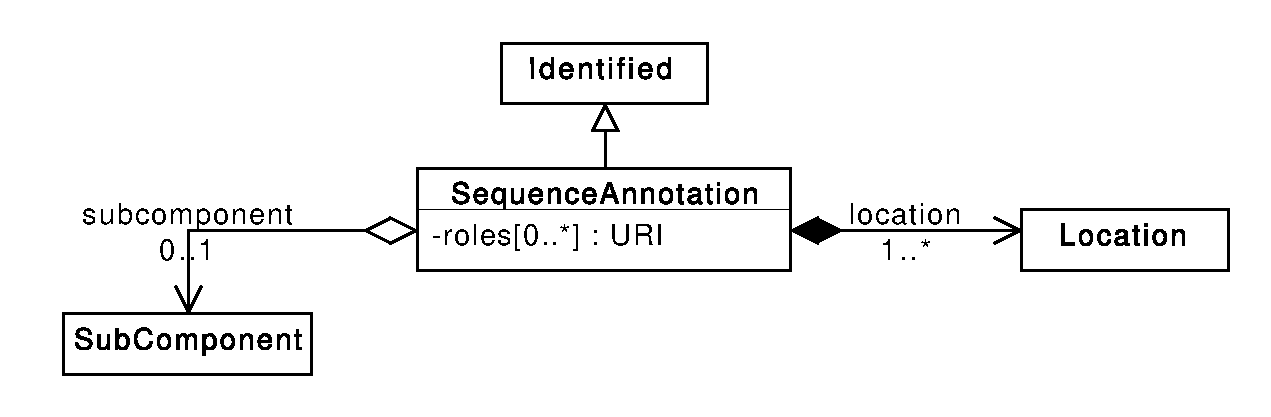
\includegraphics[scale=0.6]{uml/sequence_annotation}
\caption[]{Diagram of the \sbol{SequenceAnnotation} class and its associated properties.}
\label{uml:sequence_annotation}
\end{center}
\end{figure}

\paragraph{The \sbolheading{locations} property}\label{sec:locations}
The \sbol{locations} property is a REQUIRED set of one or more \sbol{Location} objects that indicate which \sbol{elements} of a \sbol{Sequence} are described by the \sbol{SequenceAnnotation}.

Allowing multiple \sbol{Location} objects on a single \sbol{SequenceAnnotation} is intended to enable representation of discontinuous regions (for example, a \sbol{Component} encoded across a set of exons with interspersed introns).
As such, the \sbol{Location} objects of a single \sbol{SequenceAnnotation} SHOULD NOT specify overlapping regions, since it is not clear what this would mean.
There is no such concern with different \sbol{SequenceAnnotation} objects, however, which can freely overlap in \sbol{Location} (for example, specifying overlapping linkers for sequence assembly).

\paragraph{The \sbolheading{component} property}\label{sec:component}
The \sbol{component} property is OPTIONAL and has a data type of \sbol{URI}. This \sbol{URI} MUST refer to a \sbol{Component} that is contained by the same parent \sbol{ComponentDefinition} that contains the \sbol{SequenceAnnotation}. In this way, the properties of the \sbol{SequenceAnnotation}, such as its \sbol{description} and \sbol{locations}, are associated with part of the substructure of its parent \sbol{ComponentDefinition}.

\twoonezero{
\paragraph{The \sbolheading{roles} property}\label{sec:roles:SA}
\vspace{-7pt}
\-\hspace{0.8cm}[New in 2.1.0; see SEP 004: \url{https://github.com/SynBioDex/SEPs/blob/master/sep_004.md}]\\
\-\hspace{0.8cm}[New in 2.1.0; see SEP 010: \url{https://github.com/SynBioDex/SEPs/blob/master/sep_010.md}]

Alternatively to describing substructure, a \sbol{SequenceAnnotation} can be utilized to identify a feature, such as a GenBank feature, of a specified \sbol{Sequence}.  In this use case, the \sbol{SequenceAnnotation} MUST NOT have a \sbol{component} property, but instead it would have a \sbolmult{roles:SA}{roles} property.

The \sbolmult{roles:SA}{roles} property comprises an OPTIONAL set of zero or more \sbol{URI}s describing the specified sequence feature being annotated.  If provided, these \sbolmult{roles:SA}{role} \sbol{URI}s MUST identify terms from appropriate ontologies. Roles are not restricted to describing biological function; they may annotate \sbol{Sequence}s' function in any domain for which an ontology exists.

It is RECOMMENDED that these \sbolmult{roles:SA}{role} \sbol{URI}s identify terms that are compatible with the \sbolmult{types:CD}{type} properties of this \sbol{SequenceAnnotation}'s parent \sbol{ComponentDefinition}. For example, a \sbolmult{roles:SA}{role} of a \sbol{SequenceAnnotation} which belongs to a \sbol{ComponentDefinition} of type DNA might refer to terms from the Sequence Ontology. A table of recommended ontology terms for \sbolmult{roles:SA}{roles} is given in \ref{tbl:componentdefinition_roles}.
}

\paragraph{Serialization}

\twoonezero{
The serialization of a \sbol{SequenceAnnotation} MUST have the form below. In this template, {\tt A\_LOCATION\_SUBCLASS} represents one of the \sbol{Location} subclasses.
}
\lstsetsbol
\begin{lstlisting}
<sbol:SequenceAnnotation rdf:about="...">
  ... [\emph{properties inherited from identified}] ...
  [\emph{zero or one}] <sbol:component rdf:resource="..."/> [\emph{element}]
  [\emph{one or more}] <sbol:location>
                 <sbol:A_LOCATION_SUBCLASS rdf:about="...">...</sbol:A_LOCATION_SUBCLASS>
              </sbol:location> [\emph{elements}]
  [\emph{zero or more}] <sbol:role rdf:resource="..."/> [\emph{elements}]
</sbol:SequenceAnnotation>
\end{lstlisting}

The example below shows the serialization of a \sbol{SequenceAnnotation} object. It specifies the region occupied by  a \sbol{Component} named BBa\_F2620.
\lstsetsbol
\begin{lstlisting}
<sbol:SequenceAnnotation rdf:about="http://partsregistry.org/cd/BBa_F2620/anno2">
  <sbol:persistentIdentity rdf:resource="http://partsregistry.org/cd/BBa_F2620/anno2"/>
  <sbol:displayId>anno2</sbol:displayId>
  <sbol:location>
    <sbol:Range rdf:about="http://partsregistry.org/cd/BBa_F2620/anno2/range">
      <sbol:persistentIdentity rdf:resource="http://partsregistry.org/cd/BBa_F2620/anno2/range"/>
      <sbol:displayId>range</sbol:displayId>
      <sbol:start>56</sbol:start>
      <sbol:end>68</sbol:end>
      <sbol:orientation rdf:resource="http://sbols.org/v2#inline"/>
    </sbol:Range>
  </sbol:location>
  <sbol:component rdf:resource="http://partsregistry.org/cd/BBa_F2620/rbs"/>
</sbol:SequenceAnnotation>
\end{lstlisting}

\subsubsection{Location}
\label{sec:Location}
The \sbol{Location} class is extended by the \sbol{Range}, \sbol{Cut}, and \sbol{GenericLocation} classes.

\begin{figure}[ht]
\begin{center}
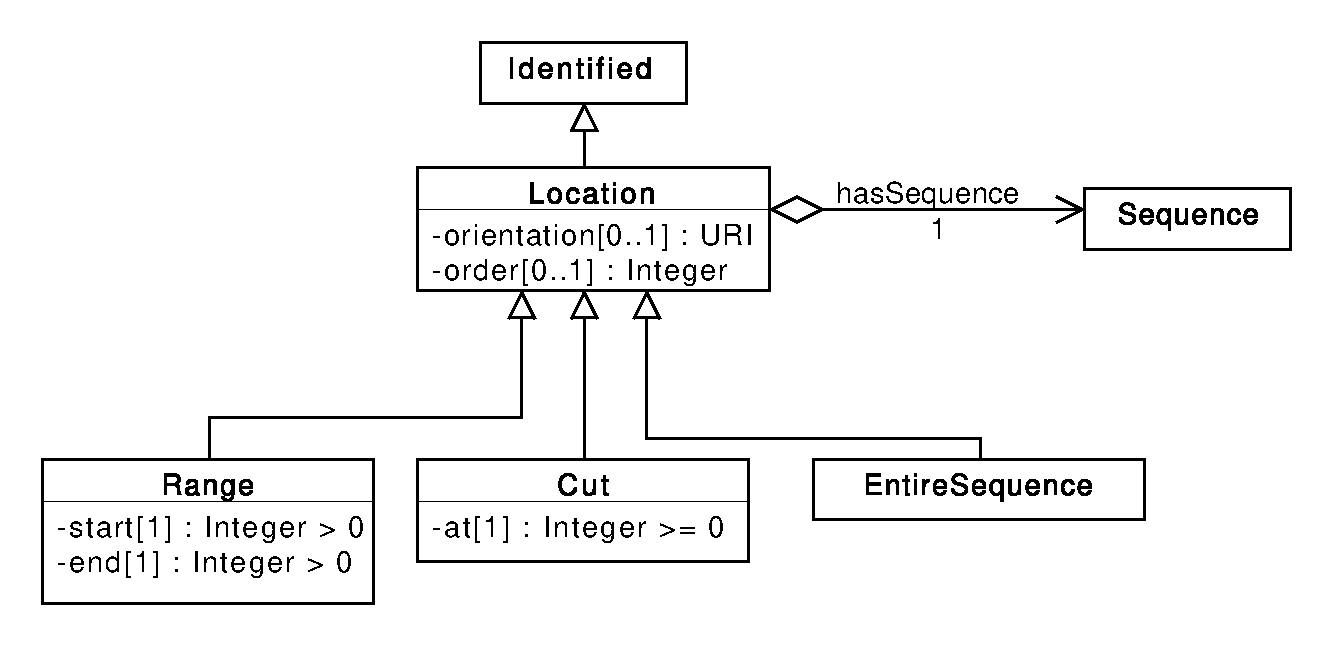
\includegraphics[scale=0.6]{uml/location}
\caption[]{Diagram of the \sbol{Location} class and its associated properties.}
\label{uml:location}
\end{center}
\end{figure}

\paragraph{The \sbolheading{orientation} property}
\label{sec:orientation}
The \sbol{orientation} property is OPTIONAL and has a data type of \sbol{URI}. All subclasses of \sbol{Location} share this property, which can be used to indicate how the region specified by the \sbol{SequenceAnnotation} and any associated double-stranded \sbol{Component} is oriented on the \sbol{elements} of a \sbol{Sequence}  from their parent \sbol{ComponentDefinition}. \ref{tbl:orientation_types} provides a list of REQUIRED \sbol{orientation} \sbol{URI}s. If a \sbol{Location} object has an \sbol{orientation}, then it MUST come from \ref{tbl:orientation_types}.

\begin{table}[ht]
  \begin{edtable}{tabular}{lp{3.75in}}
    \toprule
    \textbf{Orientation URI} & \textbf{Description} \\
    \midrule
    \url{http://sbols.org/v2\#inline} & The region specified by this \sbol{Location} is on the \sbol{elements} of a \sbol{Sequence}. \\
    \url{http://sbols.org/v2\#reverseComplement} & The region specified by this \sbol{Location} is on the reverse-complement translation of the \sbol{elements} of a \sbol{Sequence}. The exact nature of this translation depends on the \sbol{encoding} of the \sbol{Sequence}. \\
    \bottomrule
  \end{edtable}
  \caption{REQUIRED \sbol{URI}s for the \sbol{orientation} property}
  \label{tbl:orientation_types}
\end{table}


\paragraph{Range}
\label{sec:Range}
A \sbol{Range} object specifies a region via discrete, inclusive \sbol{start} and \sbol{end} positions that correspond to indices for characters in the \sbol{elements} \sbol{String} of a \sbol{Sequence}.

Note that the index of the first location is 1, as is typical practice in biology, rather than 0, as is typical practice in computer science.

\paragraph{The \sbolheading{start} property}\label{sec:start}
The \sbol{start} property specifies the inclusive starting position of the \sbol{Range}. This property is REQUIRED and MUST contain an \sbol{Integer} value greater than zero.

\paragraph{The \sbolheading{end} property}\label{sec:end}
The \sbol{end} property specifies the inclusive ending position of the \sbol{Range}. This property is REQUIRED and MUST contain an \sbol{Integer} value greater than zero. In addition, this \sbol{Integer} value MUST be greater than or equal to that of the \sbol{start} property.

\paragraph{Serialization}

The serialization of a \sbol{Range} MUST have the following form:
\lstsetsbol
\begin{lstlisting}
<sbol:Range rdf:about="...">
  ... [\emph{properties inherited from identified}] ...
  [\emph{one}]         <sbol:start>...</sbol:start> [\emph{element}]
  [\emph{one}]         <sbol:end>...</sbol:end> [\emph{element}]
  [\emph{zero or one}] <sbol:orientation rdf:resource="..."/> [\emph{element}]
</sbol:Range>
\end{lstlisting}

The example below shows the serialization of a \sbol{Range} object. It specifies the region between the inclusive positions 56 and 68, with an \sbol{orientation} of ``inline.''
\lstsetsbol
\begin{lstlisting}
<sbol:Range rdf:about="http://partsregistry.org/cd/BBa_F2620/anno2/range">
  <sbol:persistentIdentity rdf:resource="http://partsregistry.org/cd/BBa_F2620/anno2/range"/>
  <sbol:displayId>range</sbol:displayId>
  <sbol:start>56</sbol:start>
  <sbol:end>68</sbol:end>
  <sbol:orientation rdf:resource="http://sbols.org/v2#inline"/>
</sbol:Range>
\end{lstlisting}

\paragraph{Cut}
\label{sec:Cut}
The \sbol{Cut} class has been introduced to enable the specification of a region between two discrete positions.
This specification is accomplished using the \sbol{at} property, which specifies a discrete position that that corresponds to the index of a character in the \sbol{elements} \sbol{String} of a \sbol{Sequence} (except in the case when \sbol{at} is equal to zero---see below).

\paragraph{The \sbolheading{at} property}
\label{sec:at}
The \sbol{at} property is REQUIRED and MUST contain an \sbol{Integer} value greater than or equal to zero. The region specified by the \sbol{Cut} is between the position specified by this property and the position that immediately follows it. When the \sbol{at} property is equal to zero, the specified region is immediately before the first discrete position or character in the \sbol{elements} \sbol{String} of a \sbol{Sequence}.

\paragraph{Serialization}

The serialization of a \sbol{Cut} MUST have the following form:
\lstsetsbol
\begin{lstlisting}
<sbol:Cut rdf:about="...">
  ... [\emph{properties inherited from identified}] ...
  [\emph{one}]         <sbol:at>...</sbol:at> [\emph{element}]
  [\emph{zero or one}] <sbol:orientation rdf:resource="..."/> [\emph{element}]
</sbol:Cut>
\end{lstlisting}

The example below shows the serialization of a \sbol{Cut} object. It specifies a region in between positions 10 and 11, with an \sbol{orientation} of ``inline.''
\lstsetsbol
\begin{lstlisting}
<sbol:Cut rdf:about="http://partsregistry.org/cd/BBa_J23119/cutat10/cut">
  <sbol:persistentIdentity rdf:resource="http://partsregistry.org/cd/BBa_J23119/cutat10/cut"/>
  <sbol:displayId>cut</sbol:displayId>
  <sbol:at>10</sbol:at>
  <sbol:orientation rdf:resource="http://sbols.org/v2#inline"/>
</sbol:Cut>
\end{lstlisting}


\paragraph{GenericLocation}
\label{sec:GenericLocation}

While the \sbol{Range} and \sbol{Cut} classes are best suited to
specifying regions on \sbol{Sequence} objects with \external{IUPAC} encodings, the
\sbol{GenericLocation} class is included as a starting point for specifying regions on \sbol{Sequence} objects with different \sbol{encoding} properties and potentially nonlinear structure. This class can also be used to set the \sbol{orientation} of a \sbol{SequenceAnnotation} and any associated \sbol{Component} when their parent \sbol{ComponentDefinition} is a partial design that lacks a \sbol{Sequence}.

\paragraph{Serialization}

The serialization of a \sbol{GenericLocation} MUST have the following form:
\lstsetsbol
\begin{lstlisting}
<sbol:GenericLocation rdf:about="...">
  ... [\emph{properties inherited from identified}] ...
  [\emph{zero or one}] <sbol:orientation rdf:resource="..."/> [\emph{element}]
</sbol:GenericLocation>
\end{lstlisting}

The example below shows the serialization of a \sbol{GenericLocation} object with an \sbol{orientation} of ``reverse complement'':
\lstsetsbol
\begin{lstlisting}
<sbol:GenericLocation rdf:about="http://www.partsregistry.org/Part:BBa_F2620/anno5/location">
  <sbol:orientation rdf:resource="http://sbols.org/v2#reverseComplement"/>
</sbol:GenericLocation>
\end{lstlisting}

\subsubsection{SequenceConstraint}
\label{sec:SequenceConstraint}
The \sbol{SequenceConstraint} class can be used to assert restrictions on the relative, sequence-based positions of pairs of \sbol{Component} objects contained by the same parent \sbol{ComponentDefinition}.
The primary purpose of this class is to enable the specification of partially designed \sbol{ComponentDefinition} objects, for which the precise positions or orientations of their contained \sbol{Component} objects are not yet fully determined. Each \sbol{SequenceConstraint} includes the \sbol{restriction}, \sbol{subject}, and \sbol{object} properties.

\begin{figure}[ht]
\begin{center}
\includegraphics[scale=0.6]{uml/sequence_constraint}
\caption[]{Diagram of the \sbol{SequenceConstraint} class and its associated properties.}
\label{uml:sequence_constraint}
\end{center}
\end{figure}

\paragraph{The \sbolheading{subject} property}\label{sec:subject}
The \sbol{subject} property is REQUIRED and MUST contain a \sbol{URI} that refers to a \sbol{Component} contained by the same parent \sbol{ComponentDefinition} that contains the \sbol{SequenceConstraint}.

\paragraph{The \sbolheading{object} property}\label{sec:object}
The \sbol{object} property is REQUIRED and MUST contain a \sbol{URI} that refers to a \sbol{Component} contained by the same parent \sbol{ComponentDefinition} that contains the \sbol{SequenceConstraint}. This \sbol{Component} MUST NOT be the same \sbol{Component} that the \sbol{SequenceConstraint} refers to via its \sbol{subject} property.

\paragraph{The \sbolheading{restriction} property}\label{sec:restriction}

The \sbol{restriction} property is REQUIRED and has a data type of \sbol{URI}. This property MUST indicate the type of structural restriction on the positions, orientations, or structural identities of the \sbol{subject} and \sbol{object} \sbol{Component} objects in relation to each other. The \sbol{URI} value of this property SHOULD come from the RECOMMENDED \sbol{URI}s in \ref{tbl:restriction_types}.

% Note: With regards to SBOL Version 1.1., this is a generalization of former \sbol{SequenceAnnotation} property \external{precedes}.

\twotwozero{
\begin{table}[ht]
  \begin{edtable}{tabular}{lp{3.25in}}
    \toprule
    \textbf{Restriction URI} & \textbf{Description} \\
    \midrule
    \url{http://sbols.org/v2\#precedes} & The position of the \sbol{subject} \sbol{Component} MUST precede that of the \sbol{object} \sbol{Component}. If each one is associated with a \sbol{SequenceAnnotation}, then the \sbol{SequenceAnnotation} associated with the \sbol{subject} \sbol{Component} MUST specify a region that starts before the region specified by the \sbol{SequenceAnnotation} associated with the \sbol{object} \sbol{Component}. \\
    \url{http://sbols.org/v2\#sameOrientationAs} & The \sbol{subject} and \sbol{object} \sbol{Component} objects MUST have the same orientation. If each one is associated with a \sbol{SequenceAnnotation}, then the \sbol{orientation} \sbol{URI}s of the \sbol{Location} objects of the first \sbol{SequenceAnnotation} MUST be among those of the second \sbol{SequenceAnnotation}, and vice versa. \\
    \url{http://sbols.org/v2\#oppositeOrientationAs} & The \sbol{subject} and \sbol{object} \sbol{Component} objects MUST have opposite orientations. If each one is associated with a \sbol{SequenceAnnotation}, then the \sbol{orientation} \sbol{URI}s of the \sbol{Location} objects of one \sbol{SequenceAnnotation} MUST NOT be among those of the other \sbol{SequenceAnnotation}. \\
    \url{http://sbols.org/v2\#differentFrom} & The \sbolmult{definition:CI}{definition} property of the \sbol{subject} \sbol{Component} MUST NOT refer to the same \sbol{ComponentDefinition} as that of the \sbol{object} \sbol{Component}. \\
    \bottomrule
  \end{edtable}
  \caption{RECOMMENDED \sbol{URI}s for the \sbol{restriction} property.}
  \label{tbl:restriction_types}
\end{table}
}

\paragraph{Serialization}

The serialization of a \sbol{SequenceConstraint} MUST have the following form:
\lstsetsbol
\begin{lstlisting}
<sbol:SequenceConstraint rdf:about="...">
  ... [\emph{properties inherited from identified}] ...
  [\emph{one}] <sbol:restriction rdf:resource="..."/> [\emph{element}]
  [\emph{one}] <sbol:subject rdf:resource="..."/> [\emph{element}]
  [\emph{one}] <sbol:object rdf:resource="..."/> [\emph{element}]
</sbol:SequenceConstraint>
\end{lstlisting}

The example below shows the serialization of a \sbol{SequenceConstraint} belonging to the \sbol{ComponentDefinition} of a LacI-repressible promoter. This \sbol{SequenceConstraint} has a ``precedes'' \sbol{restriction} that indicates that the \sbol{subject} \sbol{Component}, which represents the core of the promoter, is positioned before the \sbol{object} \sbol{Component}, which represents the LacI operator of the promoter.
\lstsetsbol
\begin{lstlisting}
<sbol:SequenceConstraint rdf:about="http://partsregistry.org/cd/BBa_K174004/r1">
  <sbol:persistentIdentity rdf:resource="http://partsregistry.org/cd/BBa_K174004/r1"/>
  <sbol:displayId>r1</sbol:displayId>
  <sbol:restriction rdf:resource="http://sbols.org/v2#precedes"/>
  <sbol:subject rdf:resource="http://partsregistry.org/cd/pspac"/>
  <sbol:object rdf:resource="http://partsregistry.org/cd/LacI_operator"/>
</sbol:SequenceConstraint>
\end{lstlisting}

\subsection{Model}
\label{sec:Model}

\begin{figure}[ht]
\begin{center}
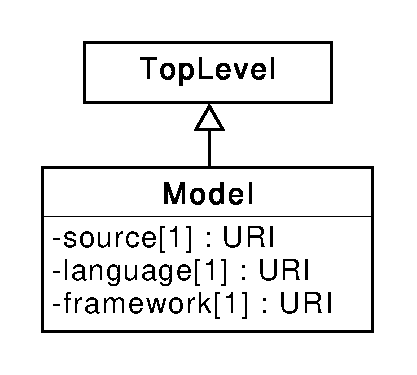
\includegraphics[scale=0.6]{uml/model}
\caption[]{Diagram of the \sbol{Model} class and its associated properties.}
\label{uml:model}
\end{center}
\end{figure}

The purpose of the \sbol{Model} class is to serve as a placeholder for an external computational model and provide additional meta-data to enable better reasoning about the contents of this model.
In this way, there is minimal duplication of standardization efforts and users of SBOL can formalize the function of a \sbol{ModuleDefinition} in the language of their choice.

The meta-data provided by the \sbol{Model} class include the following properties: the \sbolmult{source:M}{source} or location of the actual content of the model, the \sbol{language} in which the model is implemented, and the model's \sbol{framework}.

\subsubsection*{ The \sbolheading{source} property}\label{sec:source:M}
The \sbolmult{source:M}{source} property is REQUIRED and MUST contain a \sbol{URI} reference to the source file for a model.

\subsubsection*{ The \sbolheading{language} property}\label{sec:language}
The \sbol{language} property is REQUIRED and MUST contain a \sbol{URI} that specifies the language in which the model is implemented. It is RECOMMENDED that this \sbol{URI} refer to a term from the EMBRACE Data and Methods (EDAM) ontology. \ref{tbl:model_types} provides a list of terms from this ontology and their \sbol{URI}s. If the \sbol{language} property of a \sbol{Model} is well-described by one these terms, then it MUST contain the \sbol{URI} for this term as its value.

\begin{table}[ht]
  \begin{edtable}{tabular}{ll}
    \toprule
    \textbf{Model Language} & \textbf{URI for EDAM Term} \\
    \midrule
    SBML  & \url{http://identifiers.org/edam/format_2585}\\
    CellML		 & \url{http://identifiers.org/edam/format_3240}\\
    BioPAX    & \url{http://identifiers.org/edam/format_3156}\\
    \bottomrule
  \end{edtable}
  \caption{Terms from the EDAM ontology to specify the \sbol{language} property of a \sbol{Model}.}
  \label{tbl:model_types}
\end{table}


\subsubsection*{ The \sbolheading{framework} property}\label{sec:framework}
The \sbol{framework} property is REQUIRED and MUST contain a \sbol{URI} that specifies the framework in which the model is implemented.
It is RECOMMENDED this \sbol{URI} refer to a term from the modeling framework branch of the SBO when possible. A few suggested modeling frameworks and their corresponding \sbol{URI}s are shown in \ref{tbl:model_frameworks}. If the \sbol{framework} property of a \sbol{Model} is well-described by one these terms, then it MUST contain the \sbol{URI} for this term as its value.

\begin{table}[ht]
  \begin{edtable}{tabular}{ll}
    \toprule
    \textbf{Framework} & \textbf{URI for SBO Term} \\
    \midrule
    Continuous  & \url{http://identifiers.org/biomodels.sbo/SBO:0000062}\\
    Discrete & \url{http://identifiers.org/biomodels.sbo/SBO:0000063}\\
    \bottomrule
  \end{edtable}
  \caption{SBO terms to specify the \sbol{framework} property of a \sbol{Model}.}
  \label{tbl:model_frameworks}
\end{table}

\subsubsection*{Serialization}

The serialization of a \sbol{Model} MUST have the following form:

\lstsetsbol
\begin{lstlisting}
<sbol:Model rdf:about="http://www.sbolstandard.org/examples/toggleswitch">
  ... [\emph{properties inherited from identified}] ...
  [\emph{one}] <sbol:source rdf:resource="..."/> [\emph{element}]
  [\emph{one}] <sbol:language rdf:resource="..."/> [\emph{element}]
  [\emph{one}] <sbol:framework rdf:resource="..."/> [\emph{element}]
</sbol:Model>
\end{lstlisting}

The example below shows the serialization of a \sbol{Model} object that refers to a quantitative model of a genetic toggle switch. The model is implemented in the SBML \sbol{language} and adheres to a continuous modeling \sbol{framework}. Lastly, the model can be retrieved from a model repository via its \sbolmult{source:M}{source} \sbol{URI}, which is a \external{URL}.
\lstsetsbol
\begin{lstlisting}
<?xml version="1.0" ?>
<rdf:RDF xmlns:rdf="http://www.w3.org/1999/02/22-rdf-syntax-ns#" xmlns:dcterms="http://purl.org/dc/terms/" xmlns:prov="http://www.w3.org/ns/prov#" xmlns:sbol="http://sbols.org/v2#">
  <sbol:Model rdf:about="http://www.sbolstandard.org/examples/pIKE_Toggle_1">
    <sbol:persistentIdentity rdf:resource="http://www.sbolstandard.org/examples/pIKE_Toggle_1"/>
    <sbol:displayId>pIKE_Toggle_1</sbol:displayId>
    <dcterms:title>pIKE_Toggle_1 toggle switch</dcterms:title>
    <sbol:source rdf:resource="http://virtualparts.org/part/pIKE_Toggle_1"/>
    <sbol:language rdf:resource="http://identifiers.org/edam/format_2585"/>
    <sbol:framework rdf:resource="http://identifiers.org/biomodels.sbo/SBO:0000062"/>
  </sbol:Model>
</rdf:RDF>
\end{lstlisting}
\label{ser:Model}

\subsection{ModuleDefinition}
\label{sec:ModuleDefinition}

\begin{figure}[ht]
\begin{center}
\includegraphics[scale=0.6]{uml/module_definition}
\caption[]{Diagram of the \sbol{ModuleDefinition} class and its associated properties.}
\label{uml:module_definition}
\end{center}
\end{figure}

The \sbol{ModuleDefinition} class represents a grouping of structural and functional entities in a biological design. The primary usage of this class is to assert the molecular interactions and abstract function of its child entities.

As shown in \ref{uml:module_definition}, these child entities are aggregated via the \sbol{functionalComponents} \sbol{modules} properties, while representation of their abstract function is accomplished via the \sbolmult{roles:MD}{roles}  property. More detailed descriptions of the function of a \sbol{ModuleDefinition} are provided by its \sbol{interactions} and \sbol{models} properties. Lastly, since \sbol{ModuleDefinition} objects can be more abstract and represent entities of  engineering design rather than biology, they can have designated ``inputs'' and ``outputs'' expressed by the \sbol{direction} properties on its\\
\sbol{FunctionalComponent} objects.

\subsubsection*{The \sbolheading{roles} property}\label{sec:roles:MD}
The \sbolmult{roles:MD}{roles} property is an OPTIONAL set of \sbol{URI}s that clarifies the intended function of a \sbol{ModuleDefinition}.

These \sbol{URI}s might identify descriptive biological roles, such as ``metabolic pathway'' and ``signaling cascade,'' but they can also identify identify ``logical'' roles, such as ``inverter'' or ``AND gate'', or other abstract roles for describing the function of design. Interpretation of the meaning of such roles currently depends on the software tools that read and write them.

\subsubsection*{The \sbolheading{modules} property}\label{sec:modules}

The \sbol{modules} property is OPTIONAL and MAY specify a set of \sbol{Module} objects contained by the \sbol{ModuleDefinition}.
Note that the set of relations between \sbol{Module} and \sbol{ModuleDefinition} objects is strictly acyclic.

While the \sbol{ModuleDefinition} class is analogous to a specification sheet for a system of interacting biological elements, the \sbol{Module} class represents the occurrence of a particular subsystem within the system.
Hence, this class allows a system design to include multiple instances of a subsystem, all defined by reference to the same \sbol{ModuleDefinition}.
For example, consider the \sbol{ModuleDefinition} for a network of two-input repressor devices in which the particular repressors have not been chosen yet. This \sbol{ModuleDefinition} could contain multiple \sbol{Module} objects that refer to the same \sbol{ModuleDefinition} of an abstract two-input repressor device.

\subsubsection*{The \sbolheading{functionalComponents} property}
\label{sec:functionalComponents}

The \sbol{functionalComponents} property is OPTIONAL and MAY specify a set of \sbol{FunctionalComponent} objects contained by the \sbol{ModuleDefinition}.

Just as a \sbol{Module} represents an instance of a subsystem in the overall system represented by a  \sbol{ModuleDefinition}, a \sbol{FunctionalComponent} represents an instance of a structural entity (represented by a \sbol{ComponentDefinition}) in the system. This concept allows a \sbol{ModuleDefinition} to assert different interactions for separate copies of the same structural entity if needed. For example, a \sbol{ModuleDefinition} might contain multiple \sbol{FunctionalComponent}  objects that refer to the same promoter \sbol{ComponentDefinition}, but assert different interactions for these promoter copies based on their separate positions in another \sbol{ComponentDefinition} that represents the structure of the entire system.

\subsubsection*{The \sbolheading{interactions} property}\label{sec:interactions}

The \sbol{interactions} property is OPTIONAL and MAY specify a set of \sbol{Interaction} objects within the\\
\sbol{ModuleDefinition}.

The \sbol{Interaction} class provides an abstract, machine-readable representation of entity behavior within a\\ \sbol{ModuleDefinition} (whereas a more detailed model of the system might not be suited to machine reasoning, depending on its implementation).
Each \sbol{Interaction} contains \sbol{Participation} objects that indicate the roles of the \sbol{FunctionalComponent} objects involved in the \sbol{Interaction}.

\subsubsection*{The \sbolheading{models} property}\label{sec:models}
The \sbol{models} property is OPTIONAL and MAY specify a set of \sbol{URI} references to \sbol{Model} objects.

\sbol{Model} objects are placeholders that link \sbol{ModuleDefinition} objects to computational models of any format.
A \sbol{ModuleDefinition} object can link to more than one \sbol{Model} since each might encode system behavior in a different way or at a different level of detail.

\subsubsection*{Serialization}

The serialization of \sbol{ModuleDefinition} has the following form:
\lstsetsbol
\begin{lstlisting}
<sbol:ModuleDefinition rdf:about="...">
  ... [\emph{properties inherited from identified}] ...
  [\emph{zero or more}]  <sbol:role rdf:resource="..."/> [\emph{elements}]
  [\emph{zero or more}]  <sbol:model rdf:resource="..."/> [\emph{elements}]
  [\emph{zero or more}] <sbol:functionalComponent>
                 <sbol:FunctionalComponent rdf:about="...">...</sbol:FunctionalComponent >
               </sbol:functionalComponent> [\emph{elements}]
  [\emph{zero or more}] <sbol:module>
                 <sbol:Module rdf:about="...">...</sbol:Module>
               </sbol:module> [\emph{elements}]
  [\emph{zero or more}] <sbol:interaction>
                 <sbol:Interaction rdf:about="...">...</sbol:Interaction>
               </sbol:interaction> [\emph{elements}]
</sbol:ModuleDefinition>
\end{lstlisting}

The example below shows a simple \sbol{ModuleDefinition} containing two components, a \sbol{FunctionalComponent} for a DNA sequence encoding constitutive expression of GFP and another for the GFP protein expressed from this sequence, plus an interaction describing that relation.

\lstsetsbol
\begin{lstlisting}
<sbol:ModuleDefinition rdf:about="http://sbolstandard.org/example/md/GFP_expression">
  <sbol:functionalComponent>
    <sbol:FunctionalComponent rdf:about="http://sbolstandard.org/example/md/GFP_expression/GFP_protein">
      <sbol:definition rdf:resource="http://sbolstandard.org/example/GFP"/>
      <sbol:access rdf:resource="http://sbols.org/v2#public"/>
      <sbol:direction rdf:resource="http://sbols.org/v2#output"/>
    </sbol:FunctionalComponent>
  </sbol:functionalComponent>
  <sbol:functionalComponent>
    <sbol:FunctionalComponent rdf:about="http://sbolstandard.org/example/md/GFP_expression/Constitutive_GFP">
      <sbol:definition rdf:resource="http://sbolstandard.org/example/GFP_generator"/>
      <sbol:access rdf:resource="http://sbols.org/v2#public"/>
      <sbol:direction rdf:resource="http://sbols.org/v2#none"/>
    </sbol:FunctionalComponent>
  </sbol:functionalComponent>
  <sbol:interaction>
    <sbol:Interaction rdf:about="http://sbolstandard.org/example/md/GFP_expression/express_GFP">
      ...
    </sbol:Interaction>
  </sbol:interaction>
</sbol:ModuleDefinition>
\end{lstlisting}

\subsubsection{Module}
\label{sec:Module}

\begin{figure}[ht]
\begin{center}
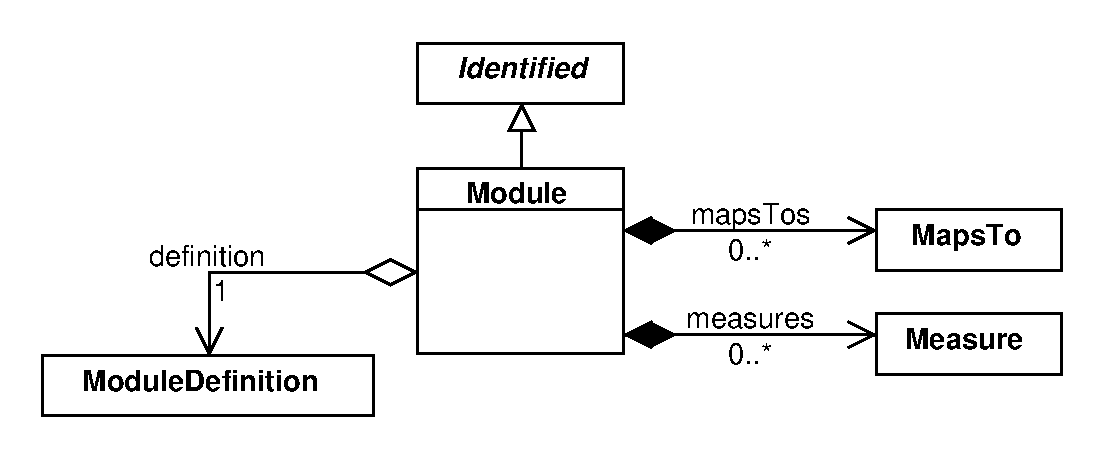
\includegraphics[scale=0.6]{uml/module}
\caption[]{Diagram of the \sbol{Module} class and its associated properties.}
\label{uml:module}
\end{center}
\end{figure}

The \sbol{Module} class represents the usage or occurrence of a \sbol{ModuleDefinition} within a larger design (that is, another \sbol{ModuleDefinition}).

\paragraph{The \sbolheading{definition} property}
\label{sec:definition:M}

The \sbolmult{definition:M}{definition} property is a REQUIRED \sbol{URI} that refers to the \sbol{ModuleDefinition} for the \sbol{Module}.

The \sbolmult{definition:M}{definition} property MUST NOT refer to the same \sbol{ModuleDefinition} as that which contains the \sbol{Module}.
Furthermore, \sbol{Module} objects MUST NOT form a cyclical chain of references via their \sbolmult{definition:M}{definition} properties and the \sbol{ModuleDefinition} objects that contain them. For example, consider the \sbol{Module} objects $A$ and $B$ and the \sbol{ModuleDefinition} objects $X$ and $Y$. The reference chain ``$X$ contains $A$, $A$ is defined by $Y$, $Y$ contains $B$, and $B$ is defined by $X$'' is cyclical.

\paragraph{The \sbolheading{mapsTo} property}
\label{sec:mapsTos:M}

The \sbolmult{mapsTos:M}{mapsTos} property is an OPTIONAL set of \sbol{MapsTo} objects that refer to and link \sbol{ComponentInstance} objects together within the heterarchy of \sbol{Module}, \sbol{ModuleDefinition}, \sbol{ComponentInstance}, and \sbol{ComponentDefinition} objects.

\ref{sec:MapsTo} contains a detailed description of the \sbol{MapsTo} class.

\paragraph{Serialization}
The serialization of \sbol{Module}s has the following form.
\lstsetsbol
\begin{lstlisting}
<sbol:Module rdf:about="...">
  ... [\emph{properties inherited from identified}] ...
  [\emph{one}]          <sbol:definition rdf:resource="..."/> [\emph{element}]
  [\emph{zero or more}] <sbol:mapsTo>
                 <sbol:MapsTo rdf:about="...">...</sbol:MapsTo>
               </sbol:mapsTo> [\emph{element}]
</sbol:Module>
\end{lstlisting}

The example below specifies a TetR inverter that is being used as
a part of a genetic toggle switch:

\lstsetsbol
\begin{lstlisting}
<sbol:Module rdf:about="http://sbolstandard.org/example/toggle_switch/tetr_inverter">
  <sbol:definition rdf:resource="http://sbolstandard.org/example/tetr_inverter"/>
  ...
</sbol:Module>
\end{lstlisting}

\subsubsection{FunctionalComponent}
\label{sec:FunctionalComponent}
A \sbol{FunctionalComponent} is an instance of a \sbol{ComponentDefinition} being used as part of a \sbol{ModuleDefinition}. The \sbol{ModuleDefinition} describes how the that describes how the \sbol{FunctionalComponent} interacts with others and summarizes their aggregate function.

The \sbol{FunctionalComponent} class inherits from the \sbol{ComponentInstance} class and therefore has the \sbolmult{definition:CI}{definition}, \sbol{access}, and \sbolmult{mapsTos:CI}{mapsTos} properties.
In addition, it has a \sbol{direction} property that specifies whether it serves as an input, output, both, or neither with regards to the \sbol{ModuleDefinition} that contains it.

\paragraph{The \sbolheading{direction} property}\label{sec:direction}
Each \sbol{FunctionalComponent} MUST specify via the \sbol{direction} property whether it serves as an  input, output, both, or neither for its parent \sbol{ModuleDefinition} object.
The value for this property MUST be one of the \sbol{URI}s given in \ref{tbl:functionalcomponent_directions}.


\begin{table}[ht]
  \begin{edtable}{tabular}{ll}
    \toprule
    \textbf{Direction URI} & \textbf{Description} \\
    \midrule

    \url{http://sbols.org/v2#in}  & Indicates that the \sbol{FunctionalComponent} is an input.\\
    \url{http://sbols.org/v2#out}  & Indicates that the \sbol{FunctionalComponent} is an output.\\
   \url{http://sbols.org/v2#inout}  & Indicates that the \sbol{FunctionalComponent} is both an input and output\\ \url{http://sbols.org/v2#none}  & Indicates that the \sbol{FunctionalComponent} is neither an input or output.\\
    \bottomrule
  \end{edtable}
  \caption{REQUIRED \sbol{URI}s for the \sbol{direction} property.}
  \label{tbl:functionalcomponent_directions}
\end{table}

The \sbol{direction} property is a means to encode how a  designer thinks about the ``purpose'' of a connection in a system.  In SBOL, such a connection is represented with a \sbol{FunctionalComponent}, and a system is represented as  with a \sbol{ModuleDefinition}.
For example, consider a system that has been designed to sense the concentration of the cell-to-cell signaling molecule 3OC$_6$HSL and report it via the concentration of another gene product.
In this system, the concentration of 3OC$_6$HSL is being sensed by the system, so the \sbol{FunctionalComponent} for 3OC$_6$HSL would have a \sbol{direction} of ``input.''
In turn, the concentration of the reporter gene product is intended to be read/consumed by other biological systems, so the \sbol{FunctionalComponent} for this product would have a \sbol{direction} of ``output.''
The CDS encoding the product, however, is not intended to directly transfer information into or out of the \sbol{ModuleDefinition} for the system, so its \sbol{FunctionalComponent} would have a \sbol{direction} of ``neither.''

\paragraph{Serialization}

The serialization of a \sbol{FunctionalComponent} has the following form.
\lstsetsbol
\begin{lstlisting}
<sbol:FunctionalComponent rdf:about="...">
  ... [\emph{properties inherited from identified}] ...
  [\emph{one}]          <sbol:definition rdf:resource="..."/> [\emph{element}]
  [\emph{one}]          <sbol:access rdf:resource="..."/> [\emph{element}]
  [\emph{one}]          <sbol:direction rdf:resource="..."/> [\emph{element}]
  [\emph{zero or more}] <sbol:mapsTo rdf:resource="..."/> [\emph{elements}]
</sbol:FunctionalComponent>
\end{lstlisting}

In the example below, the functional component is defined as a public input/output. The component refers to the \texttt{Part:BBa\_R0010} promoter from the iGEM Parts Registry.
\lstsetsbol
\begin{lstlisting}
<sbol:FunctionalComponent rdf:about="http://sbolstandard.org/example/laci_inverter/promoter">
  <sbol:definition rdf:resource="http://www.partsregistry.org/BBa_R0010"/>
  <sbol:access rdf:resource="http://sbols.org/v2#public"/>
  <sbol:direction rdf:resource="http://sbols.org/v2#inout"/>
</sbol:FunctionalComponent>
\end{lstlisting}

\subsubsection{Interaction}
\label{sec:Interaction}

\begin{figure}[ht]
\begin{center}
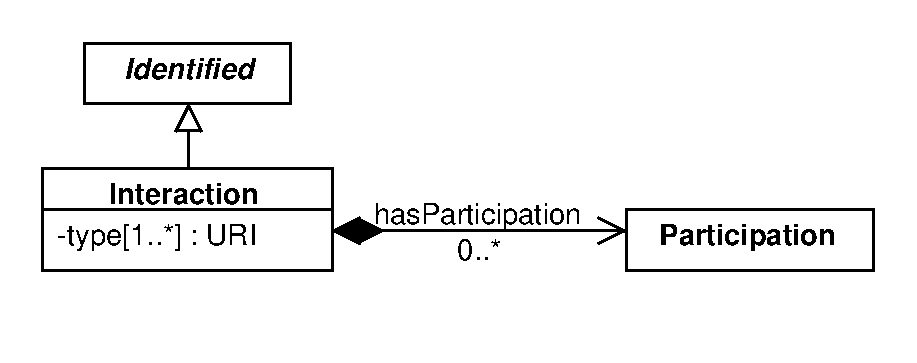
\includegraphics[scale=0.6]{uml/interaction}
\caption[]{Diagram of the \sbol{Interaction} class and its associated properties.}
\label{uml:interaction}
\end{center}
\end{figure}

The \sbol{Interaction} class provides more detailed description of how the \sbol{FunctionalComponent} objects of a\\ \sbol{ModuleDefinition} are intended to work together.
For example, this class can be used to represent different forms of genetic regulation (e.g., transcriptional activation or repression), processes from the central dogma of biology (e.g. transcription and translation), and other basic molecular interactions (e.g., non-covalent binding or enzymatic phosphorylation).
Each \sbol{Interaction} includes a \sbolmult{types:I}{types} property that refers to descriptive ontology terms and a \sbol{participations} property that describes which \sbol{FunctionalComponent} objects participate in the \sbol{Interaction}.

\paragraph{The \sbolheading{types} property}\label{sec:types:I}

The \sbolmult{types:I}{types} property is a REQUIRED set of \sbol{URI}s that describes the behavior represented by an \sbol{Interaction}.

The \sbolmult{types:I}{types} property MUST contain one or more \sbol{URI}s that MUST identify terms from appropriate ontologies. It is RECOMMENDED that \twozeroone{exactly one \sbol{URI}} contained by the \sbolmult{types:I}{types} property refer to a term from the occurring entity branch of the Systems Biology Ontology (SBO). (See \url{http://www.ebi.ac.uk/sbo/main/}) \ref{tbl:interaction_types} provides a list of possible SBO terms for the \sbolmult{types:I}{types} property and their corresponding \sbol{URI}s.

\twozeroone{
\begin{table}[ht]
  \begin{edtable}{tabular}{ll}
    \toprule
    \textbf{Interaction Type} & \textbf{URI for SBO Term} \\
    \midrule
    Inhibition  & \url{http://identifiers.org/biomodels.sbo/SBO:0000169}\\
    Stimulation & \url{http://identifiers.org/biomodels.sbo/SBO:0000170}\\
    Biochemical Reaction & \url{http://identifiers.org/biomodels.sbo/SBO:0000176}\\
    Non-Covalent Binding & \url{http://identifiers.org/biomodels.sbo/SBO:0000177}\\
    Degradation & \url{http://identifiers.org/biomodels.sbo/SBO:0000179}\\
    Genetic Production & \url{http://identifiers.org/biomodels.sbo/SBO:0000589}\\
    Control  & \url{http://identifiers.org/biomodels.sbo/SBO:0000168} \\
    \bottomrule
  \end{edtable}
  \caption{SBO terms to specify the \sbolmult{types:I}{types} property of an \sbol{Interaction}.}
  \label{tbl:interaction_types}
\end{table}
}

If an \sbol{Interaction} is well described by one of the terms from \ref{tbl:interaction_types}, then its \sbolmult{types:I}{types} property MUST contain the \sbol{URI} that identifies this term. Lastly, if the \sbolmult{types:I}{types} property of an \sbol{Interaction} contains multiple
 \sbol{URI}s, then they MUST identify non-conflicting terms. For example, the SBO terms ``stimulation'' and ``inhibition'' would conflict.

\paragraph{The \sbolheading{participations} property}\label{sec:participations}

The \sbol{participations} property is an OPTIONAL and MAY contain a set of \sbol{Participation} objects, each of which identifies the \sbolmult{roles:P}{roles} that its referenced \sbol{FunctionalComponent} plays in the \sbol{Interaction}.

Even though an \sbol{Interaction} generally contains at least one \sbol{Participation}, the case of zero \sbol{Participation} objects is allowed because it is plausible that a designer might want to specify that an \sbol{Interaction} will exist, even if its \sbol{participant}s have not yet been determined.

\paragraph{Serialization}

The serialization of an \sbol{Interaction} has the following form.
\lstsetsbol
\begin{lstlisting}
<sbol:Interaction rdf:about="...">
  ... [\emph{properties inherited from identified}] ...
  [\emph{one or more}]  <sbol:type rdf:resource="..."/> [\emph{elements}]
  [\emph{zero or more}] <sbol:participation>
                 <sbol:Participation rdf:about="...">...</sbol:Participation>
               </sbol:participation> [\emph{elements}]
</sbol:Interaction>
\end{lstlisting}

The example below shows an \sbol{Interaction} representing an inhibition relationship (SBO:0000169) between a repressor (SBO:0000020, full \sbol{Participation} details shown) and a promoter:

\lstsetsbol
\begin{lstlisting}
<sbol:Interaction rdf:about="http://sbolstandard.org/example/laci_inverter/LacI_pLacI">
  <sbol:type rdf:resource="http://identifiers.org/biomodels.sbo/SBO:0000169"/>
  <sbol:participation>
    <sbol:Participation rdf:about="http://sbolstandard.org/example/laci_inverter/LacI_pLacI/P03023">
      <sbol:role rdf:resource="http://identifiers.org/biomodels.sbo/SBO:0000020"/>
      <sbol:participant rdf:resource="http://sbolstandard.org/example/laci_inverter/TF"/>
    </sbol:Participation>
  </sbol:participation>
  <sbol:participation>
    <sbol:Participation rdf:about="...">
      ...
    </sbol:Participation>
  </sbol:participation>
</sbol:Interaction>
\end{lstlisting}

\twozeroone{
\begin{figure}[ht]
\begin{center}
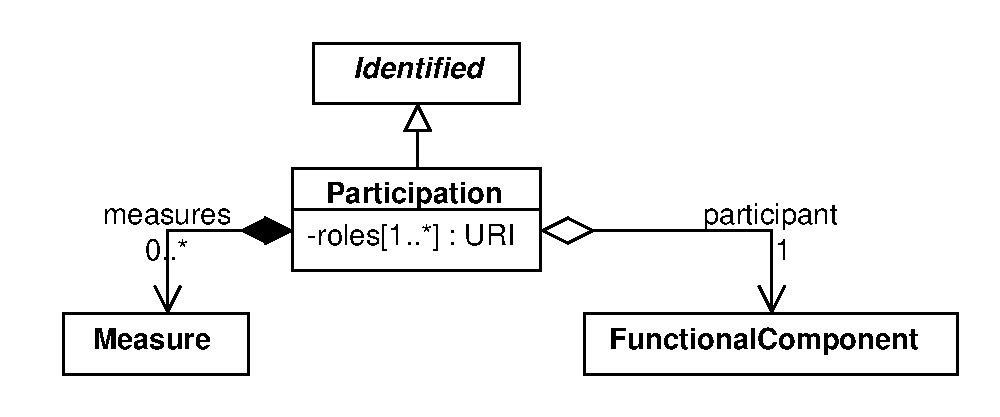
\includegraphics[scale=0.6]{uml/participation}
\caption[]{Diagram of the \sbol{Participation} class and its associated properties.}
\label{uml:participation}
\end{center}
\end{figure}
}

\subsubsection{Participation}
\label{sec:Participation}

Each \sbol{Participation} represents how a particular \sbol{FunctionalComponent} behaves in its parent
\sbol{Interaction}.

\paragraph{The \sbolheading{roles} property}\label{sec:roles:P}

\twozeroone{The \sbolmult{roles:P}{roles} property is a REQUIRED set of \sbol{URI}s that describes the behavior of a \sbol{Participation} (and by extension its referenced \sbol{FunctionalComponent}) in the context of its parent \sbol{Interaction}.

The \sbolmult{roles:P}{roles} property MUST contain one or more \sbol{URI}s that MUST identify terms from appropriate ontologies. It is RECOMMENDED that exactly one \sbol{URI} contained by the \sbolmult{roles:P}{roles} property refer to a term from the participant role branch of the SBO.} \ref{tbl:participant_roles} provides a list of possible SBO terms for the \sbolmult{roles:P}{roles} property and their corresponding \sbol{URI}s.

\begin{table}[ht]
  \begin{edtable}{tabular}{lll}
    \toprule
    \textbf{Participation Role} & \textbf{URI for SBO Term} & \textbf{Interaction Types}\\
    \midrule
    Inhibitor  & \url{http://identifiers.org/biomodels.sbo/SBO:0000020} & Inhibition\\
    Inhibited  & \url{http://identifiers.org/biomodels.sbo/SBO:0000642} & Inhibition\\
    Stimulator & \url{http://identifiers.org/biomodels.sbo/SBO:0000459}  & Stimulation\\
    Stimulated & \url{http://identifiers.org/biomodels.sbo/SBO:0000643}  & Stimulation\\
     Reactant & \url{http://identifiers.org/biomodels.sbo/SBO:0000010}  & Non-Covalent Binding, Degradation \\
     & & Biochemical Reaction \\
    Product & \url{http://identifiers.org/biomodels.sbo/SBO:0000011}  & Non-Covalent Binding, \\
    & & Genetic Production, Biochemical Reaction\\
    Promoter  & \url{http://identifiers.org/biomodels.sbo/SBO:0000598} & Inhibition, Stimulation, Genetic Production\\
    Modifier  & \url{http://identifiers.org/biomodels.sbo/SBO:0000019} & Biochemical Reaction, Control\\
    Modified  & \url{http://identifiers.org/biomodels.sbo/SBO:0000644} & Biochemical Reaction, Control\\
    Template  & \url{http://identifiers.org/biomodels.sbo/SBO:0000645} & Genetic Production\\
%    Ligand & \url{http://identifiers.org/biomodels.sbo/SBO:0000280}\\
%    Non-Covalent Complex & \url{http://identifiers.org/biomodels.sbo/SBO:0000253}\\
    \bottomrule
  \end{edtable}
  \caption{SBO terms to specify the \sbolmult{roles:P}{roles} property of a \sbol{Participation}.}
  \label{tbl:participant_roles}
\end{table}

If a \sbol{Participation} is well described by one of the terms from \ref{tbl:participant_roles}, then its \sbolmult{roles:P}{roles} property MUST contain the \sbol{URI} that identifies this term.
\twozeroone{Also, if a \sbol{Participation} belongs to an \sbol{Interaction} that has a type listed in \ref{tbl:interaction_types}, then the \sbol{Participation} SHOULD have a role that is cross-listed with this type in \ref{tbl:participant_roles}.}
Lastly, if the \sbolmult{roles:P}{roles} property of a \sbol{Participation} contains multiple
 \sbol{URI}s, then they MUST identify non-conflicting terms. For example, the SBO terms ``stimulator'' and ``inhibitor'' would conflict.


\paragraph{The \sbolheading{participant} property}\label{sec:participant}

The \sbol{participant} property MUST specify precisely one \sbol{FunctionalComponent} object that plays the designated role in its parent \sbol{Interaction} object.


\paragraph{Serialization}

The serialization of \sbol{Participation} objects has the following form.
\lstsetsbol
\begin{lstlisting}
<sbol:Participation rdf:about="...">
  ... [\emph{properties inherited from identified}] ...
  [\emph{zero or more}] <sbol:role rdf:resource="..."/> [\emph{elements}]
  [\emph{one}]          <sbol:participant rdf:resource="..."/> [\emph{element}]
</sbol:Participation>
\end{lstlisting}

In the example below, the role of participating \sbol{FunctionalComponent} is defined to be \external{inhibitor}, using the \external{SBO:0000020} term. This component is specified using the \sbol{participant} property of the \sbol{Participation} entity.
\lstsetsbol
\begin{lstlisting}
<sbol:Participation rdf:about="http://sbolstandard.org/example/laci_inverter/LacI_pLacI/P03023">
  <sbol:role rdf:resource="http://identifiers.org/biomodels.sbo/SBO:0000020"/>
  <sbol:participant rdf:resource="http://sbolstandard.org/example/laci_inverter/TF"/>
</sbol:Participation>
\end{lstlisting}

\subsection {Collection}
\label{sec:Collection}
The \sbol{Collection} class is a class that groups together a set of \sbol{TopLevel} objects that have something in common.
Some examples of \sbol{Collection} objects:
\begin{itemize}
\item Results of a query to find all \sbol{ComponentDefinition} objects in a repository that function as promoters.
\item A set of \sbol{ModuleDefinition} objects representing a library of genetic logic gates.
\item A \sbol{ModuleDefinition} for a complex design, and all of the \sbol{ModuleDefinition}, \sbol{ComponentDefinition},\\ \sbol{Sequence}, and \sbol{Model} objects used to provide its full specification.
\end{itemize}

\begin{figure}[ht]
\begin{center}
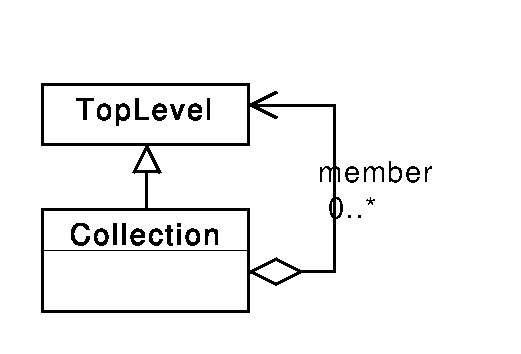
\includegraphics[scale=0.6]{uml/collection}
\caption[]{Diagram of the \sbol{Collection} class and its associated properties.}
\label{uml:collection}
\end{center}
\end{figure}

\subsubsection*{The \sbolheading{members} property}\label{sec:members}
The \sbol{members} property of a \sbol{Collection} is OPTIONAL and MAY contain a set of \sbol{URI} references to zero or more \sbol{TopLevel} objects.

\subsubsection*{Serialization}

The serialization of a \sbol{Collection} has the following form:

\lstsetsbol
\begin{lstlisting}
<sbol:Collection rdf:about="...">
  ... [\emph{properties inherited from identified}] ...
  [\emph{zero or more}] <sbol:member rdf:resource="..."/> [\emph{element}]
</sbol:Collection>
\end{lstlisting}

The example below shows the serialization of a \sbol{Collection} object grouping together a library of constitutive promoters.
\lstsetsbol
\begin{lstlisting}
<?xml version="1.0" ?>
<rdf:RDF xmlns:rdf="http://www.w3.org/1999/02/22-rdf-syntax-ns#" xmlns:dcterms="http://purl.org/dc/terms/" xmlns:prov="http://www.w3.org/ns/prov#" xmlns:sbol="http://sbols.org/v2#">
  <sbol:Collection rdf:about="http://parts.igem.org/Promoters/Catalog/Anderson">
    <sbol:persistentIdentity rdf:resource="http://parts.igem.org/Promoters/Catalog/Anderson"/>
    <sbol:displayId>Anderson</sbol:displayId>
    <dcterms:title>Anderson promoters</dcterms:title>
    <dcterms:description>The Anderson promoter collection</dcterms:description>
    <sbol:member rdf:resource="http://partsregistry.org/Part:BBa_J23119"/>
    ...
    <sbol:member rdf:resource="http://partsregistry.org/Part:BBa_J23118"/>
  </sbol:Collection>
</rdf:RDF>
\end{lstlisting}
\label{ser:Collection}

\twotwozero{
\subsection{CombinatorialDerivation}
\label{sec:CombinatorialDerivation}
\vspace{-7pt}
\-\hspace{0.8cm}[New in 2.2.0; see SEP 007: \url{https://github.com/SynBioDex/SEPs/blob/master/sep_007.md}]

The purpose of the \sbol{CombinatorialDerivation} class is to specify combinatorial genetic designs without having to specify every possible design variant. For example, a \sbol{CombinatorialDerivation} can be used to specify a library of reporter gene variants that include different promoters and RBSs without having to specify a \sbol{ComponentDefinition} for every possible combination of promoter, RBS, and CDS in the library. \sbol{ComponentDefinition} objects that realize a \sbol{CombinatorialDerivation} can be derived in accordance with the class properties \sbol{template}, \\
\sbol{variableComponents}, and \sbol{strategy} (see \ref{uml:combinatorial_derivation}).

\begin{figure}[ht]
\begin{center}
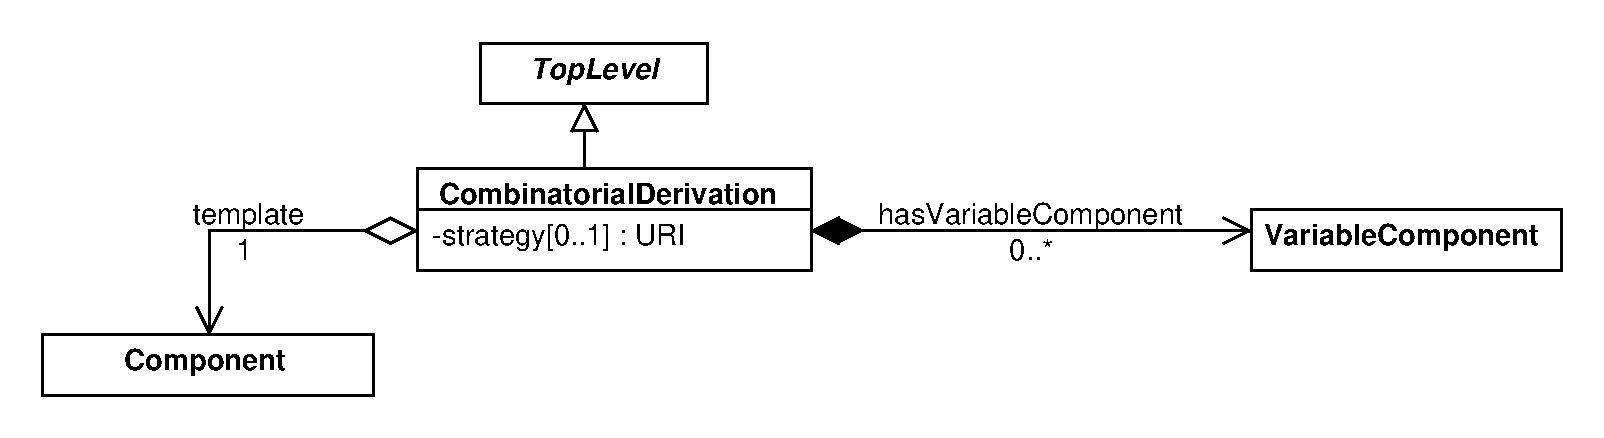
\includegraphics[scale=0.6]{uml/combinatorial_derivation}
\caption[]{Diagram of the \sbol{CombinatorialDerivation} class and its associated properties.}
\label{uml:combinatorial_derivation}
\end{center}
\end{figure}

\subsubsection*{ The \sbolheading{template} property}\label{sec:template}

The \sbol{template} property is REQUIRED and MUST contain a URI that refers to a \sbol{ComponentDefinition}. This \sbol{ComponentDefinition} is expected to serve as a template for the derivation of new \sbol{ComponentDefinition} objects. Consequently, its \sbol{components} property SHOULD contain one or more \sbol{Component} objects that describe its substructure (referred to hereafter as template \sbol{Component} objects), and its \sbol{sequenceConstraints} property MAY also contain one or more \sbol{SequenceConstraint} objects that constrain this substructure.

When a \sbol{ComponentDefinition} is derived in accordance with a \sbol{CombinatorialDerivation}, the \sbol{wasDerivedFroms} property of the derived \sbol{ComponentDefinition} SHOULD refer to the \sbol{CombinatorialDerivation}. When multiple \sbol{ComponentDefinition} objects are derived in accordance with the same \sbol{CombinatorialDerivation}, they MAY be referred to by the \sbol{members} property of a \sbol{Collection}, in which case the \sbol{wasDerivedFroms} property of the \sbol{Collection} SHOULD also refer to this \sbol{CombinatorialDerivation}.

If the \sbolmult{types:CD}{types} property of the template \sbol{ComponentDefinition} contains one or more URIs, then the \sbolmult{types:CD}{types} property of the derived \sbol{ComponentDefinition} SHOULD also contain those URIs. The same holds true for the \sbolmult{roles:CD}{roles} properties of these \sbol{ComponentDefinition} objects.

\subsubsection*{ The \sbolheading{variableComponents} property}\label{sec:variableComponents}

The \sbol{variableComponents} property is OPTIONAL and MAY contain a set of \sbol{VariableComponent} objects. These \sbol{VariableComponent} objects are expected to denote the choices available when deriving the substructure of a new \sbol{ComponentDefinition} in accordance with a \sbol{CombinatorialDerivation}. The \sbol{variableComponents} property MUST NOT contain two or more \sbol{VariableComponent} objects that refer to the same template \sbol{Component} via their \sbol{variable} properties.

If the \sbol{variable} property of one of these \sbol{VariableComponent} objects refers to a template \sbol{Component}, then the \sbol{components} property of the derived \sbol{ComponentDefinition} SHOULD contain as many \sbol{Component} objects derived from the template \sbol{Component} as specified by the \sbol{operator} property of the \sbol{VariableComponent} (see \ref{tbl:operator}). In addition, the \sbolmult{definition:CI}{definition} properties of these derived \sbol{Component} objects MUST refer to \sbol{ComponentDefinition} objects specified by the \sbol{variants}, \sbol{variantCollections}, or \sbol{variantDerivations} property of the \sbol{VariableComponent}.

If no \sbol{variable} property of one of these \sbol{VariableComponent} objects refers to a template \sbol{Component}, then the \sbol{components} property of the derived \sbol{ComponentDefinition} SHOULD contain exactly one \sbol{Component} with a \sbol{wasDerivedFroms} property that refers to the template \sbol{Component}. The \sbolmult{definition:CI}{definition} property of this derived \sbol{Component} MUST refer to the \sbol{ComponentDefinition} referred to by the \sbolmult{definition:CI}{definition} property of the template \sbol{Component}.

Finally, all of these derived \sbol{Component} objects MUST follow the \sbol{restriction} properties of any \\
\sbol{SequenceConstraint} objects that refer to their corresponding template \sbol{Component} objects.

\subsubsection*{ The \sbolheading{strategy} property}\label{sec:strategy}
The \sbol{strategy} property is OPTIONAL and has a data type of URI. \ref{tbl:strategy} provides a list of REQUIRED \sbol{strategy} URIs. If the \sbol{strategy} property is not empty, then it MUST contain a URI from \ref{tbl:strategy}. This property recommends how many \sbol{ComponentDefinition} objects a user SHOULD derive from the template \sbol{ComponentDefinition}.

}

\begin{table}[ht]
  \begin{edtable}{tabular}{lp{4in}}
    \toprule
    \textbf{Strategy URI} & \textbf{Description} \\
    \midrule
    \url{http://sbols.org/v2#enumerate}  &  A user SHOULD derive all possible \sbol{ComponentDefinition} objects specified by the \sbol{CombinatorialDerivation}. \\
        \url{http://sbols.org/v2#sample}  & A user SHOULD derive a subset of all possible \sbol{ComponentDefinition} objects specified by \sbol{CombinatorialDerivation}. The manner in which this subset is chosen is for the user to decide. \\
    \bottomrule
  \end{edtable}
  \caption{REQUIRED \sbol{URI}s for the \sbol{strategy} property.}
  \label{tbl:strategy}
\end{table}

\twotwozero{
\subsubsection*{Serialization}

The serialization of a \sbol{CombinatorialDerivation} MUST have the following form:

}

\lstsetsbol
\begin{lstlisting}
<sbol:CombinatorialDerivation rdf:about="...">
  ... [\emph{properties inherited from identified}] ...
  [\emph{one}] <sbol:template rdf:resource="..."/> [\emph{element}]
  [\emph{zero or more}]  <sbol:variableComponent>
                 <sbol:VariableComponent rdf:about="...">...</sbol:VariableComponent>
               </sbol:variableComponent> [\emph{elements}]
  [\emph{zero or one}] <sbol:strategy rdf:resource="..."/> [\emph{element}]
</sbol:CombinatorialDerivation>
\end{lstlisting}

\twotwozero{
The example below shows the serialization of a \sbol{CombinatorialDerivation} that specifies the combinatorial design for a library of GFP reporter variants. Each GFP reporter \sbol{ComponentDefinition} sampled from this\\ \sbol{CombinatorialDerivation} would be driven by one of two possible glucose-sensitive promoters and contain one GFP variant from a library of CDSs.

}

\lstsetsbol
\begin{lstlisting}
<?xml version="1.0" ?>
<rdf:RDF xmlns:rdf="http://www.w3.org/1999/02/22-rdf-syntax-ns#" xmlns:dcterms="http://purl.org/dc/terms/" xmlns:prov="http://www.w3.org/ns/prov#" xmlns:sbol="http://sbols.org/v2#">
  <sbol:CombinatorialDerivation rdf:about="http://www.sbolstandard.org/gfp_reporter_derivation/1.0.0">
    <sbol:persistentIdentity rdf:resource="http://www.sbolstandard.org/gfp_reporter_derivation"/>
    <sbol:displayId>gfp_reporter_derivation</sbol:displayId>
    <dcterms:title>GFP Reporter Derivation</dcterms:title>
    <sbol:template rdf:resource="http://www.sbolstandard.org/gfp_reporter_template/1.0.0"/>
    <sbol:strategy rdf:resource="http://sbols.org/v2#sample"/>
    <sbol:variableComponent>
      <sbol:VariableComponent rdf:about="http://www.sbolstandard.org/gfp_reporter_derivation/promoter_variable/1.0.0">
        <sbol:operator rdf:resource="http://sbols.org/v2#one"/>
        <sbol:variable rdf:resource="http://www.sbolstandard.org/gfp_reporter_template/p1/1.0.0"/>
        <sbol:variant rdf:resource="http://www.sbolstandard.org/glucose_sensitive_1/1.0.0"/>
        <sbol:variant rdf:resource="http://www.sbolstandard.org/glucose_sensitive_2/1.0.0"/>
      </sbol:VariableComponent>
    </sbol:variableComponent>
    <sbol:variableComponent>
      <sbol:VariableComponent rdf:about="http://www.sbolstandard.org/gfp_reporter_derivation/cds_variable/1.0.0">
        <sbol:operator rdf:resource="http://sbols.org/v2#one"/>
        <sbol:variable rdf:resource="http://www.sbolstandard.org/gfp_reporter_template/c1/1.0.0"/>
        <sbol:variantCollection rdf:resource="http://www.sbolstandard.org/gfp_cds_library/1.0.0"/>
      </sbol:VariableComponent>
    </sbol:variableComponent>
  </sbol:CombinatorialDerivation>
</rdf:RDF>
\end{lstlisting}

%\label{ser:Attachment}

\twotwozero{
\subsubsection{VariableComponent}
\label{sec:VariableComponent}

The \sbol{VariableComponent} class can be used to specify a choice of \sbol{ComponentDefinition} objects for any new \sbol{Component} derived from a template \sbol{Component} in the template \sbol{ComponentDefinition}. This specification is made using the class properties \sbol{variable}, \sbol{variants}, \sbol{variantCollections}, and \sbol{variantDerivations} (see \ref{uml:variable_component}). While the \sbol{variants}, \sbol{variantCollections}, and \sbol{variantDerivations} properties are OPTIONAL, at least one of them MUST NOT be empty. If these properties contain duplicate URIs, then they SHOULD be treated as a single URI for the purpose of selection. For example, if the \sbol{variants} property contains two copies of URI $A$ and one copy of URI $B$, $A$ SHOULD NOT be selected twice during enumeration, and it SHOULD NOT be selected twice as much as $B$ during sampling.

\begin{figure}[ht]
\begin{center}
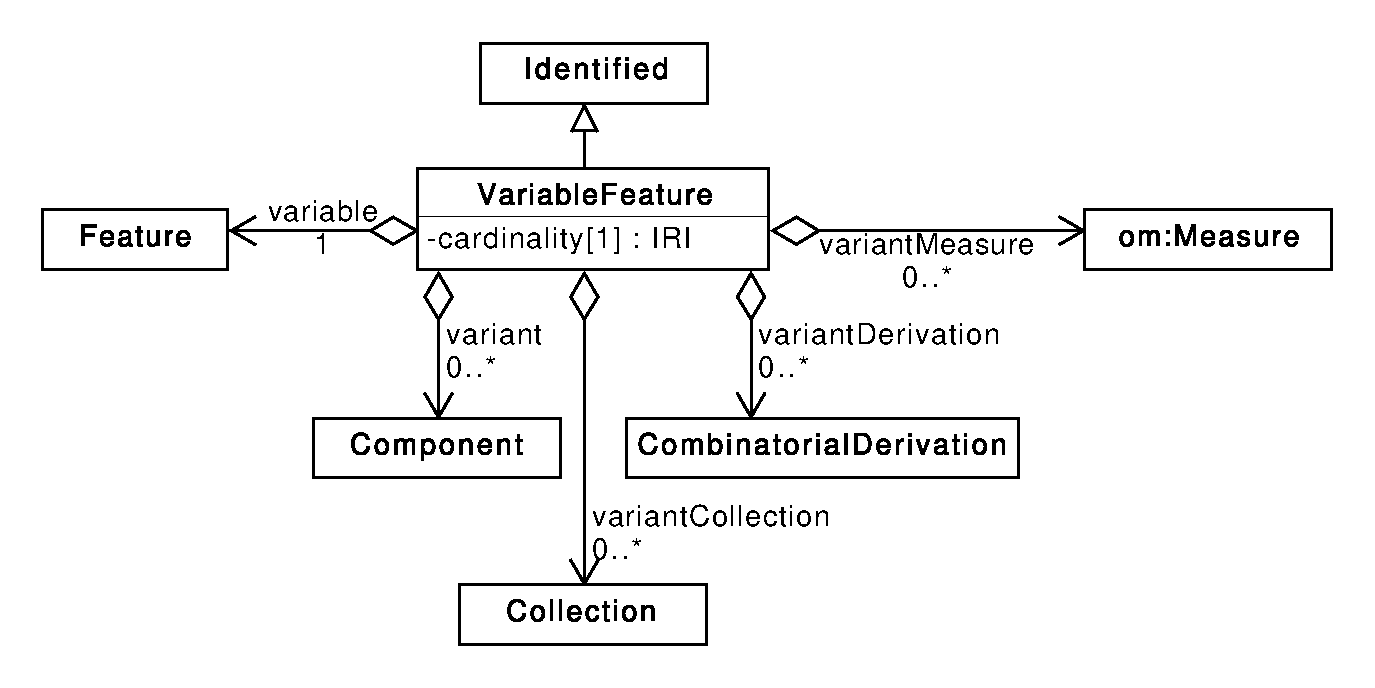
\includegraphics[scale=0.6]{uml/variable_component}
\caption[]{Diagram of the \sbol{VariableComponent} class and its associated properties.}
\label{uml:variable_component}
\end{center}
\end{figure}

\subsubsection*{ The \sbolheading{variable} property}\label{sec:variable}

The \sbol{variable} property is REQUIRED and MUST contain a URI that refers to a template \sbol{Component} in the template \sbol{ComponentDefinition}. If the \sbol{wasDerivedFroms} property of a \sbol{Component} refers to this template \sbol{Component}, then the \sbolmult{definition:CI}{definition} property of the derived \sbol{Component} MUST refer to either (1) a \sbol{ComponentDefinition} referred to by the \sbol{variants} property of the \sbol{VariableComponent}, (2) a \sbol{ComponentDefinition} from a \sbol{Collection} referred to by the \sbol{variantCollections} property of the \sbol{VariableComponent}, or (3) a \sbol{ComponentDefinition} derived from a \sbol{CombinatorialDerivation} referred to by the \sbol{variantDerivations} property of the \sbol{VariableComponent}.

If the \sbolmult{roles:CD}{roles} property of the template \sbol{Component} contains one or more URIs, then the \sbolmult{roles:CD}{roles} property of the derived \sbol{Component} SHOULD also contain those URIs.

\subsubsection*{ The \sbolheading{variants} property}\label{sec:variants}

The \sbol{variants} property is OPTIONAL and MAY contain zero or more URIs that each refer to a \sbol{ComponentDefinition}. This property specifies individual \sbol{ComponentDefinition} objects to serve as options when deriving a new\\
\sbol{Component} from the template \sbol{Component}.

\subsubsection*{ The \sbolheading{variantCollections} property}\label{sec:variantCollections}

The \sbol{variantCollections} property is OPTIONAL and MAY contain zero or more URIs that each refer to a\\
\sbol{Collection}. The \sbol{members} property of each \sbol{Collection} referred to in this way MUST NOT be empty. This property enables the convenient specification of existing groups of \sbol{ComponentDefinition} objects to serve as options when deriving a new \sbol{Component} from the template \sbol{Component}.

\subsubsection*{ The \sbolheading{variantDerivations} property}\label{sec:variantDerivations}

The \sbol{variantDerivations} property is OPTIONAL and MAY contain zero or more URIs that each refer to a\\ \sbol{CombinatorialDerivation}. This property enables the convenient specification of \sbol{ComponentDefinition} objects derived in accordance with another \sbol{CombinatorialDerivation} to serve as options when deriving a new \sbol{Component} from the template \sbol{Component}. The \sbol{variantDerivations} property of a \sbol{VariableComponent} MUST NOT refer to the \sbol{CombinatorialDerivation} that contains this \sbol{VariableComponent}. Furthermore, \sbol{VariableComponent} objects MUST NOT form a cyclical chain of references via their \sbol{variantDerivations} properties and the\\ \sbol{CombinatorialDerivation} objects that contain them. For example, consider the \sbol{VariableComponent} objects A and B and the \sbol{CombinatorialDerivation} objects X and Y. The reference chain X contains A, A has variant derivation Y, Y contains B, and B has variant derivation X is cyclical.

\subsubsection*{ The \sbolheading{operator} property}\label{sec:operator}

The \sbol{operator} property is REQUIRED and has a data type of URI. This property specifies how many \sbol{Component} objects SHOULD be derived from the template \sbol{Component} during the derivation of a new \sbol{ComponentDefinition}. The URI value of this property MUST come from the URIs provided in~\ref{tbl:operator}.

}

\begin{table}[ht]
  \begin{edtable}{tabular}{lp{4in}}
    \toprule
    \textbf{Operator URI} & \textbf{Description} \\
    \midrule
    \url{http://sbols.org/v2#zeroOrOne} & No more than one \sbol{Component} in the derived \sbol{ComponentDefinition} SHOULD have a \sbol{wasDerivedFroms} property that refers to the template \sbol{Component}. \\
        \url{http://sbols.org/v2#one} & Exactly one \sbol{Component} in the derived \sbol{ComponentDefinition} SHOULD have a \sbol{wasDerivedFroms} property that refers to the template \sbol{Component}. \\
\url{http://sbols.org/v2#zeroOrMore} & Any number of \sbol{Component} objects in the derived \sbol{ComponentDefinition} MAY have \sbol{wasDerivedFroms} properties that refer to the template \sbol{Component}. \\
\url{http://sbols.org/v2#oneOrMore} & At least one \sbol{Component} in the derived \sbol{ComponentDefinition} SHOULD have a \sbol{wasDerivedFroms} property that refers to the template \sbol{Component}. \\
    \bottomrule
  \end{edtable}
  \caption{REQUIRED \sbol{URI}s for the \sbol{operator} property.}
  \label{tbl:operator}
\end{table}

\twotwozero{
\subsubsection*{Serialization}

The serialization of a \sbol{VariableComponent} MUST have the following form:

}

\lstsetsbol
\begin{lstlisting}
<sbol:VariableComponent rdf:about="...">
  ... [\emph{properties inherited from identified}] ...
  [\emph{one}] <sbol:variable rdf:resource="..."/> [\emph{element}]
  [\emph{zero or more}] <sbol:variant rdf:resource="..."/> [\emph{element}]
  [\emph{zero or more}] <sbol:variantCollection rdf:resource="..."/> [\emph{element}]
  [\emph{zero or more}] <sbol:variantDerivation rdf:resource="..."/> [\emph{element}]
  [\emph{one}] <sbol:operator rdf:resource="..."/> [\emph{element}]
</sbol:VariableComponent>
\end{lstlisting}

\twotwozero{
The example below shows the serialization of a \sbol{VariableComponent} that specifies a choice of one or more operator sites from a library of variants for the derivation of a synthetic CMV promoter.

}

\lstsetsbol
\begin{lstlisting}
<sbol:VariableComponent rdf:about="http://www.sbolstandard.org/cmv_promoter_derivation/operator_variable/1.0.0">
  <sbol:operator rdf:resource="http://sbols.org/v2#oneOrMore"/>
  <sbol:variable rdf:resource="http://www.sbolstandard.org/cmv_promoter_template/o1/1.0.0"/>
  <sbol:variantCollection rdf:resource="http://www.sbolstandard.org/operator_library/1.0.0"/>
</sbol:VariableComponent>
\end{lstlisting}

\twotwozero{
\subsection{Implementation}
\label{sec:Implementation}
\vspace{-7pt}
\-\hspace{0.8cm}[New in 2.2.0; see SEP 019: \url{https://github.com/SynBioDex/SEPs/blob/master/sep_019.md}]

An \sbol{Implementation} represents an instance of a synthetic biological construct, and describes the build phase of a design-built-test-learn workflow. Importantly, an \sbol{Implementation} can be associated with a laboratory sample that was already built, or that is to be built in the future. An \sbol{Implementation} can also represent virtual and simulated instances.  An \sbol{Implementation} may be linked back to its original design (either a \sbol{ModuleDefinition} or \sbol{ComponentDefinition}) using the \sbol{wasDerivedFroms} property inherited from the \sbol{Identified} superclass. An \sbol{Implementation} may also link to a \sbol{ModuleDefinition} or \sbol{ComponentDefinition} that specifies its realized structure and/or function.
% as described in Section2.1.1.

\begin{figure}[ht]
\begin{center}
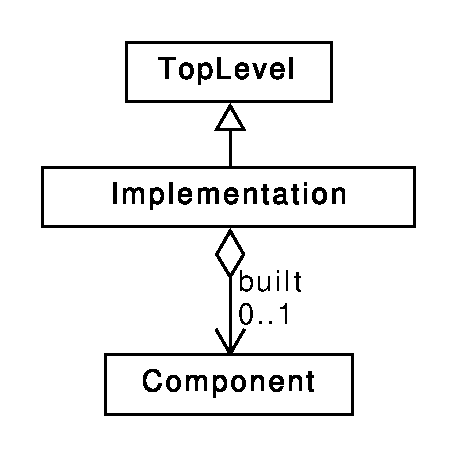
\includegraphics[scale=0.5]{uml/implementation}
\caption[]{Diagram of the \sbol{Implementation} class and its associated properties.}
\label{uml:implementation}
\end{center}
\end{figure}

\subsubsection*{ The \sbolheading{built} property}\label{sec:built}
The \sbol{built} property is OPTIONAL and MAY contain a URI that MUST refer to a \sbol{TopLevel} object that is either a \sbol{ComponentDefinition} or \sbol{ModuleDefinition}. This \sbol{ComponentDefinition} or \sbol{ModuleDefinition} is intended to describe the actual physical structure and/or functional behavior of the \sbol{Implementation}. When the built property refers to a \sbol{ComponentDefinition} or \sbol{ModuleDefinition} that is also linked to the \sbol{Implementation} via PROV-O properties such as \sbol{wasDerivedFroms} (see \ref{sec:provenance}), it can be inferred that the actual structure and/or function of the \sbol{Implementation} matches its original design. When the \sbol{built} property refers to a different \sbol{ComponentDefinition} or \sbol{ModuleDefinition}, it can be inferred that the \sbol{Implementation} has deviated from the original design. For example, the latter could be used to document when the DNA sequencing results for an assembled construct do not match the original target sequence.
}

\twotwozero{
\subsubsection*{Serialization}

The serialization of an \sbol{Implementation} has the following form:
}
\lstsetsbol
\begin{lstlisting}
<sbol:Implementation rdf:about="...">
  ... [\emph{properties inherited from Identified}] ...
  [\emph{one}]          <sbol:built rdf:resource="..."/> [\emph{element}]
</sbol:Implementation>
\end{lstlisting}

\twotwozero{
 In the example below, an \sbol{Implementation} links back to its target design via the \sbol{wasDerivedFroms} property. Since this particular sample did not match its target structure when synthesized in the lab, a \sbol{ComponentDefinition} representing its mutated structure is linked by the \sbol{built} field.
}

\lstsetsbol
\begin{lstlisting}
  <sbol:Implementation rdf:about="http://examples.org/Implementation/build/1.0.0">
   <sbol:displayId>build</sbol:displayId>
    <sbol:persistentIdentity rdf:resource="http://examples.org/Implementation/build"/>
    <sbol:version>1.0.0</sbol:version>
    <prov:wasDerivedFrom rdf:resource="http://examples.org/ComponentDefinition/design/1.0.0"/>
    <sbol:built rdf:resource="http://examples.org/ComponentDefinition/mutant/1.0.0"/>
  </sbol:Implementation>
\end{lstlisting}

\twotwozero{
\subsection{Attachment}
\label{sec:Attachment}
\vspace{-7pt}
\-\hspace{0.8cm}[New in 2.2.0; see SEP 018: \url{https://github.com/SynBioDex/SEPs/blob/master/sep_018.md}]

\begin{figure}[ht]
\begin{center}
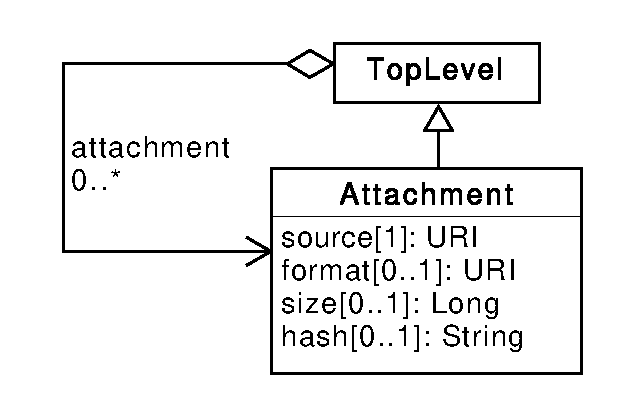
\includegraphics[scale=0.6]{uml/attachment}
\caption[]{Diagram of the \sbol{Attachment} class and its associated properties.}
\label{uml:attachment}
\end{center}
\end{figure}

The purpose of the \sbol{Attachment} class is to serve as a general container for data files, especially experimental data files.
It provides a means for linking files and metadata to SBOL designs.

The meta-data provided by the \sbol{Attachment} class include the following properties: the \sbolmult{source:A}{source} or location of the actual file of the attachment, the \sbol{format} of the file, the \sbol{size} of the file, and the \sbol{hash} for the file.

\subsubsection*{ The \sbolheading{source} property}\label{sec:source:A}
The \sbolmult{source:A}{source} property is REQUIRED and MUST contain a \sbol{URI} reference to the source file.

\subsubsection*{ The \sbolheading{format} property}\label{sec:format}
The \sbol{format} property is OPTIONAL and MAY contain a \sbol{URI} that specifies the format of the attached file. It is RECOMMENDED that this \sbol{URI} refer to a term from the EMBRACE Data and Methods (EDAM) ontology.

\subsubsection*{ The \sbolheading{size} property}\label{sec:size}
The \sbol{size} property is OPTIONAL and MAY contain a long indicating the file size in bytes.

\subsubsection*{ The \sbolheading{hash} property}\label{sec:hash}
The \sbol{hash} property is OPTIONAL and MAY contain a SHA-1 hash of the file contents represented as a hexadecimal digest.

\subsubsection*{Serialization}

The serialization of an \sbol{Attachment} MUST have the following form:

}

\lstsetsbol
\begin{lstlisting}
<sbol:Attachment rdf:about="...">
  ... [\emph{properties inherited from identified}] ...
  [\emph{one}] <sbol:source rdf:resource="..."/> [\emph{element}]
  [\emph{zero or one}] <sbol:format rdf:resource="..."/> [\emph{element}]
  [\emph{zero or one}] <sbol:size>...</sbol:size> [\emph{element}]
  [\emph{zero or one}] <sbol:hash>...</sbol:hash> [\emph{element}]
</sbol:Attachment>
\end{lstlisting}

\twotwozero{
The example below shows the serialization of an \sbol{Attachment} object that refers to a PNG file containing a plot of simulation data.  The attachment in this example can be retrieved from a repository via its \sbolmult{source:A}{source} \sbol{URI}, which is a \external{URL}.
}
\lstsetsbol
\begin{lstlisting}
<?xml version="1.0" ?>
<rdf:RDF xmlns:rdf="http://www.w3.org/1999/02/22-rdf-syntax-ns#" xmlns:dcterms="http://purl.org/dc/terms/" xmlns:prov="http://www.w3.org/ns/prov#" xmlns:sbol="http://sbols.org/v2#">
  <sbol:Attachment rdf:about="https://synbiohub.org/public/ACS_SynBio/attachment_00009Les8pDTQCmKA7A5T6">
    <sbol:persistentIdentity rdf:resource="https://synbiohub.org/public/ACS_SynBio/attachment_00009Les8pDTQCmKA7A5T6"/>
    <sbol:displayId>attachment_00009Les8pDTQCmKA7A5T6</sbol:displayId>
    <dcterms:title>NicePlot.png</dcterms:title>
    <sbol:source rdf:resource="https://synbiohub.org/public/ACS_SynBio/attachment_00009Les8pDTQCmKA7A5T6/1/download"/>
    <sbol:format rdf:resource="http://identifiers.org/edam/format_3603"/>
    <sbol:size>31399</sbol:size>
    <sbol:hash>404966a5062857f63edb5c3ba16bb581d7fb6a1e</sbol:hash>
  </sbol:Attachment>
</rdf:RDF>
\end{lstlisting}
\label{ser:Attachment}

\subsection{Annotation and Extension of SBOL}
\label{sec:Annotations}

SBOL does not currently represent all types of biological design data, since many of these data types (e.g., biological context and design performance metrics) lack a clear consensus on their proper representation. In addition, some types of biological data are not directly relevant to design and are therefore outside of the scope of SBOL.

To enable representation of these data, SBOL allows developers to embed custom data within SBOL objects and documents, such that these data can be exchanged without being damaged or lost. This annotation and extension mechanism is designed to enable new types of data to be easily incorporated into the SBOL standard once there is community consensus on their proper representation.

Several methods are supported for connecting the SBOL data model with other types of application-specific data:
\begin{itemize}
\item Custom data can be added to an SBOL object by annotating that object with non-conflicting properties. These properties could contain \sbol{literal} data types such as \sbol{String}s or \sbol{URI}s that require a resolution mechanism to obtain external data. An example is annotating a \sbol{ComponentDefinition} with  a property that contains a \sbol{String} description and \sbol{URI} for the parts registry from which its source data was originally imported.
\item Custom data in the form of independent objects can be added to an SBOL document by  creating\\
\sbol{GenericTopLevel} objects and annotating them as described above. An example is a \sbol{GenericTopLevel} object that is annotated such that it represents a data sheet that describes the performance of a \sbol{ModuleDefinition} in a particular context.
\item Finally, just as custom objects can be embedded in an  SBOL document, external documents can embed or refer to SBOL objects. Support for this last case is not explicitly provided in this specification. Rather, this case depends on the external non-SBOL system managing its relationship to SBOL and data serialized in RDF/XML, and is included here for completeness.
\end{itemize}

\subsubsection{Annotating SBOL objects}
% whole set of labels for the properties defined herein
\label{sec:qName}
\label{sec:QName}
\label{sec:value}
\label{sec:Annotation}
\label{sec:AnnotationValue}
\label{sec:NestedAnnotations}
\label{sec:nestedQName}
\label{sec:nestedURI}

Each \sbol{Identified} object MAY contain any number of \sbol{Annotation} objects that store data in the form of name/value property pairs. The \sbol{qName} is REQUIRED and MUST contain a \sbol{QName}, which is composed of a namespace, an OPTIONAL prefix, and a local name. The \sbol{qName} property MUST be stored in the data model to allow for proper serialization as described below.
The \sbol{value} property is also REQUIRED and MUST contain a \sbol{literal} (i.e., a \sbol{String}, \sbol{Integer}, \sbol{Double}, \sbol{Boolean}), \sbol{URI}, or \sbol{NestedAnnotations} object. A \sbol{NestedAnnotations} object MUST contain \sbol{nestedQName} and \sbol{nestedURI} properties, and it MAY contain an \sbol{annotations} property that contains zero or more \sbol{Annotation} objects.

\begin{figure}[!ht]
\begin{center}
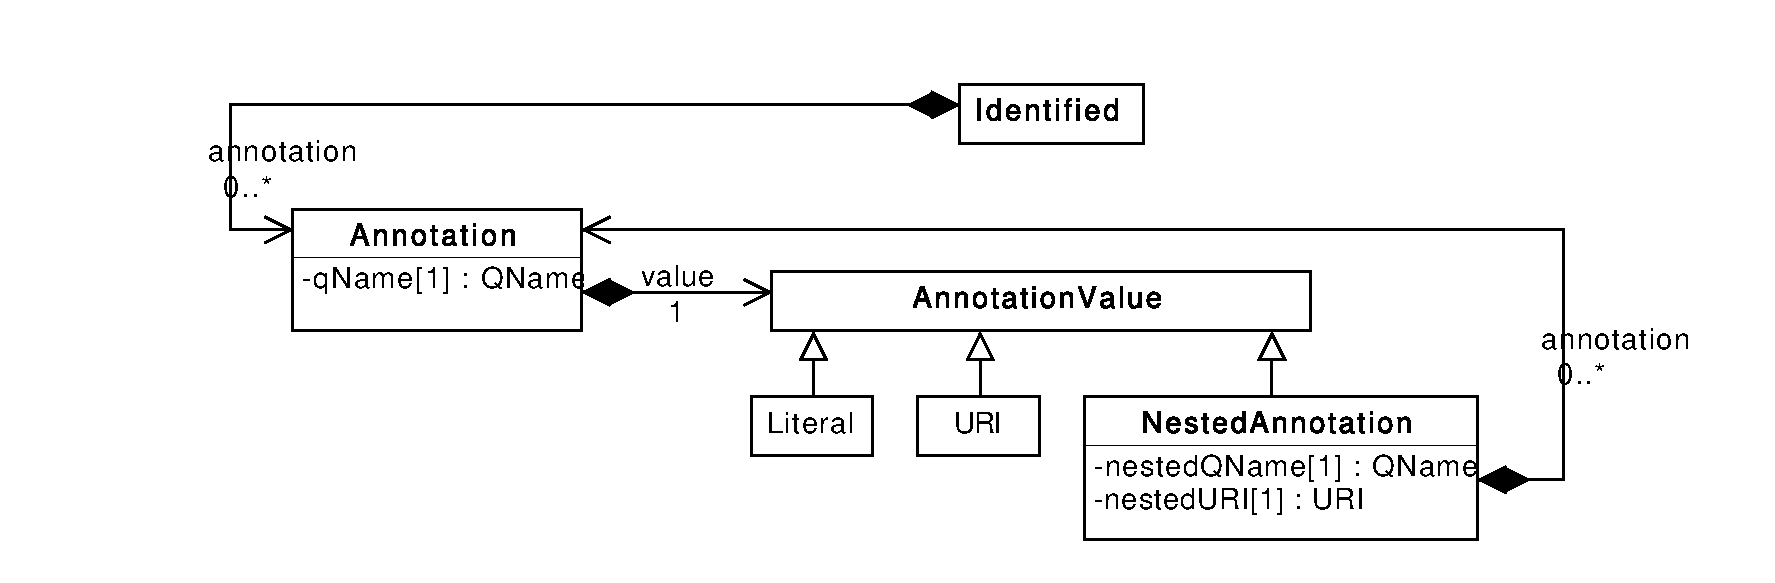
\includegraphics[scale=0.525]{uml/identified_annotations}
\caption[]{Diagram of the \sbol{Annotation} class and its association with \sbol{Identified} and \sbol{AnnotationValue} objects, which is used for annotating SBOL entities with application specific data.}
\label{uml:identified_annotations}
\end{center}
\end{figure}

\subsubsection*{Serialization}

The serialization of an \sbol{Annotation} has the following form:

\lstsetsbol
\begin{lstlisting}
<?xml version="1.0" ?>
<rdf:RDF xmlns:rdf="http://www.w3.org/1999/02/22-rdf-syntax-ns#"
  xmlns:sbol="http://sbols.org/v2#"
  xmlns:prefix1="NAMESPACE_1"
  xmlns:prefix2="NAMESPACE_2"
  xmlns:nestedObjectPrefix="A_NESTED_OBJECT_NAMESPACE"
  ...
 >
<sbol:A_TOPLEVELOBJECT rdf:about="...">
                ...
  [\emph{zero or more}] <prefix1:LOCAL_NAME_1>A_LITERAL</prefix1:LOCAL_NAME_1> [\emph{elements}]
  [\emph{zero or more}] <prefix1:LOCAL_NAME_2 rdf:resource=URI/> [\emph{elements}]
  [\emph{zero or more}] <prefix2:LOCAL_NAME_3>
                  <nestedObjectPrefix:NESTED_LOCAL_NAME rdf:about="...">
                    ...
                  </nestedObjectPrefix:NESTED_LOCAL_NAME>
                </prefix2:LOCAL_NAME_3> [\emph{elements}]
</sbol:TOPLEVELOBJECT>
\end{lstlisting}
The \sbol{qName} property specifies a namespace, prefix, and local part/name. The use of such qualified names is described in detail by the W3C (\url{http://www.w3.org/TR/1999/REC-xml-names-19990114/#ns-using}). Essentially, the ``xmlns'' property defines the prefix \sbol{String} to use as an alias for the namespace.  The prefix can be any \sbol{String}. Its use is OPTIONAL, since it simply replaces the full namespace, thereby making the serialization easier for a human to read.

The first form of \sbol{Annotation} shown above is for an \sbol{Annotation} that contains a \sbol{literal} as its \sbol{value}. The second form is for an  \sbol{Annotation} that contains a \sbol{URI} as its value. Finally, the third form is for an \sbol{Annotation} that contains a  \sbol{NestedAnnotations} object as its value. In the last case, the \sbol{nestedQName} property specifies the nested namespace, nested prefix, and nested local part/name, while the \sbol{nestedURI} property species the \sbol{URI} for the \sbol{NestedAnnotations} object.

The example below shows how the serialization for a promoter \sbol{ComponentDefinition} can be annotated with custom data. \sbol{Annotation}s are added containing the relevant information from the iGEM Parts Registry. Each property serialization of an \sbol{Annotation} is qualified with the \external{http://www.partsregistry.org/} namespace, which is prefixed using \external{pr}. The first \sbol{Annotation} is named \external{pr:group}. It specifies the iGEM group that has designed the promoter and has a \sbol{String} value.
The second \sbol{Annotation} is named \external{pr:experience}. It contains a \sbol{URI} value that is serialized as an RDF resource and can be resolved to the information Web page on the Parts Registry for the promoter.
Finally, the third \sbol{Annotation} is named \external{pr:information}. It contains a \sbol{NestedAnnotations} object that is serialized as shown and includes information about the regulatory details of the promoter using \sbol{Annotations} that correspond to Parts Registry categories.

\begin{figure} [ht]
\lstsetsbol
\begin{lstlisting}
<?xml version="1.0" ?>
<rdf:RDF xmlns:pr="http://partsregistry.org/" xmlns:rdf="http://www.w3.org/1999/02/22-rdf-syntax-ns#" xmlns:dcterms="http://purl.org/dc/terms/" xmlns:prov="http://www.w3.org/ns/prov#" xmlns:sbol="http://sbols.org/v2#">
  <sbol:ComponentDefinition rdf:about="http://partsregistry.org/cd/BBa_J23119">
    <sbol:persistentIdentity rdf:resource="http://partsregistry.org/cd/BBa_J23119"/>
    <sbol:displayId>BBa_J23119</sbol:displayId>
    <pr:group>iGEM2006_Berkeley</pr:group>
    <pr:experience rdf:resource="http://parts.igem.org/cgi/partsdb/part_info.cgi?part_name=BBa_J23119"/>
    <pr:information>
      <pr:Information rdf:about="http://partsregistry.org/cd/BBa_J23119/information">
        <pr:sigmafactor>//rnap/prokaryote/ecoli/sigma70</pr:sigmafactor>
        <pr:regulation>//regulation/constitutive</pr:regulation>
      </pr:Information>
    </pr:information>
    <dcterms:title>J23119</dcterms:title>
    <dcterms:description>Constitutive promoter</dcterms:description>
    <sbol:type rdf:resource="http://www.biopax.org/release/biopax-level3.owl#DnaRegion"/>
    <sbol:role rdf:resource="http://identifiers.org/so/SO:0000167"/>
  </sbol:ComponentDefinition>
</rdf:RDF>
\end{lstlisting}
\label{ser:Annotation}
\end{figure}

\subsubsection{GenericTopLevel}
\label{sec:GenericTopLevel}
\label{sec:rdfType}

Custom data can also be embedded at the top level of an SBOL document. The \sbol{GenericTopLevel} class is used to represent top-level entities whose purpose is to contain a set of annotations that are independent of any other class of SBOL object.
Entities that have independent existence and are not recognized by the SBOL standard are deserialized to \sbol{GenericTopLevel} objects.
These \sbol{GenericTopLevel} objects can be safely used by tools to exchange non-SBOL data.

As with other \sbol{TopLevel} objects, \sbol{GenericTopLevel} objects MAY include the properties \sbol{displayId}, \sbol{name},\\ \sbol{description}, etc. The type of data annotating a \sbol{GenericTopLevel} object is indicated using the REQUIRED \sbol{rdfType} property, which MUST contain a \sbol{QName}. As before with the \sbol{qName} property, the \sbol{rdfType} property is used to set the namespace, prefix, and local part/name during serialization.

\begin{figure}[ht]
\begin{center}
\includegraphics[scale=0.6]{uml/generictoplevel}
\caption[]{Diagram of the \sbol{GenericTopLevel} class and its associated properties, which is used for embedding externally defined entities into SBOL documents.}
\label{uml:generictoplevel}
\end{center}
\end{figure}

\subsubsection*{Serialization}

The serialization of the \sbol{GenericTopLevel} class has the following form, where the prefix, namespace, and local part/name are defined by the \sbol{rdfType} property:

%<?xml version="1.0" ?>
%<rdf:RDF ... xmlns:prefix=namespace ...>
%<prefix:localPart rdf:about="...">
%              ...
%</prefix:localPart>

\lstsetsbol
\begin{lstlisting}
<?xml version="1.0" ?>
<rdf:RDF xmlns:rdf="http://www.w3.org/1999/02/22-rdf-syntax-ns#"
  xmlns:sbol="http://sbols.org/v2#"
  xmlns:applicationPrefix="APPLICATION_NAMESPACE"
  ...
 >
<applicationPrefix:APPLICATION_OBJECT_NAME rdf:about="...">
  ... [\emph{properties inherited from identified}] ...
  ... [\emph{any non-conflicting application-specific properties}] ...
</applicationPrefix:APPLICATION_OBJECT_NAME>
\end{lstlisting}

The example below shows how a datasheet object can be added to an SBOL document using the \sbol{GenericTopLevel} class.
The J23119 promoter \sbol{ComponentDefinition} is annotated with the \external{myapp:datasheet} property that contains the \sbol{URI} of a \sbol{TopLevel} Datasheet object. The Datasheet object is further annotated with the transcription rate and \sbol{URI} for the actual characterization data using the \external{myapp:transcriptionRate} and \external{myapp:characterizationData} properties, respectively. As specified by their \sbol{rdfType} and \sbol{qName} properties, the \sbol{TopLevel} Datasheet object and all \sbol{Annotation} objects in this example are serialized with the custom \external{\path{http://www.myapp.org/}} namespace and \external{myapp} prefix.

\begin{figure}[ht]
\lstsetsbol
\begin{lstlisting}
<?xml version="1.0" ?>
<rdf:RDF xmlns:myapp="http://www.myapp.org/" xmlns:rdf="http://www.w3.org/1999/02/22-rdf-syntax-ns#" xmlns:dcterms="http://purl.org/dc/terms/" xmlns:prov="http://www.w3.org/ns/prov#" xmlns:sbol="http://sbols.org/v2#">
  <sbol:ComponentDefinition rdf:about="http://www.partsregistry.org/cd/BBa_J23119">
    <sbol:persistentIdentity rdf:resource="http://www.partsregistry.org/cd/BBa_J23119"/>
    <sbol:displayId>BBa_J23119</sbol:displayId>
    <prov:wasDerivedFrom rdf:resource="http://www.partsregistry.org/Part:BBa_J23119"/>
    <myapp:datasheet rdf:resource="http://www.partsregistry.org/gen/datasheet1"/>
    <dcterms:title>J23119</dcterms:title>
    <dcterms:description>Constitutive promoter</dcterms:description>
    <sbol:type rdf:resource="http://www.biopax.org/release/biopax-level3.owl#DnaRegion"/>
    <sbol:role rdf:resource="http://identifiers.org/so/SO:0000167"/>
  </sbol:ComponentDefinition>
  <myapp:Datasheet rdf:about="http://www.partsregistry.org/gen/datasheet1">
    <sbol:persistentIdentity rdf:resource="http://www.partsregistry.org/gen/datasheet1"/>
    <sbol:displayId>datasheet1</sbol:displayId>
    <myapp:characterizationData rdf:resource="http://www.myapp.org/measurement/1"/>
    <myapp:transcriptionRate>1</myapp:transcriptionRate>
    <dcterms:title>Datasheet 1</dcterms:title>
  </myapp:Datasheet>
</rdf:RDF>
\end{lstlisting}
\label{ser:GenericTopLevel}
\end{figure}

\section{Mapping Between SBOL 1.1 and SBOL 2.x}
\label{sec:mapping}

\ref{SBOL1TO2} depicts the mapping of SBOL 1.1 classes to SBOL 2.x classes, indicating corresponding classes/properties by color.
The SBOL 2.x \sbol{Model} and \sbol{ModuleDefinition} classes have no SBOL 1.1 equivalent, and thus are not shown.
In particular:
\begin{itemize}
\item SBOL 1.1 \external{Collection} objects containing \external{DnaComponent} objects map to SBOL 2.x \sbol{Collection} objects that contain \sbol{ComponentDefinition} objects with DNA \sbolmult{types:CD}{types} properties.
\item SBOL 1.1 \external{DnaComponent} objects maps to SBOL 2.x \sbol{ComponentDefinition} objects with DNA \sbolmult{types:CD}{types} properties.
\item SBOL 1.1 \external{DnaSequence} objects maps to an SBOL 2.x \sbol{Sequence} objects with \external{IUPAC DNA} \sbol{encoding} properties.
\item SBOL 1.1 \external{SequenceAnnotation} objects with \external{bioStart} and \external{bioEnd} properties map to SBOL 2.x\\
\sbol{SequenceAnnotation} objects that contain \sbol{Range} objects.
\item SBOL 1.1 \external{SequenceAnnotation} objects that lack \external{bioStart} and \external{bioEnd} properties map to an SBOL 2.x \sbol{SequenceAnnotation} objects that contain \sbol{GenericLocation} objects.
\item Each SBOL 1.1 \external{SequenceAnnotation} also maps to an SBOL 2.x \sbol{Component}, which represents the instantiation or usage of the appropriate \sbol{ComponentDefinition}.
\item Each SBOL 1.1 \external{precedes} property maps to an SBOL 2.x \sbol{SequenceConstraint} that specifies a precedes \sbol{restriction} property.
\end{itemize}

\begin{figure*}[h]
\begin{center}
  \includegraphics[width=\textwidth]{images/sbol_v1_to_v2}
\end{center}
\caption{\label{SBOL1TO2}The mapping from the SBOL 1.1 data model to the SBOL 2.x  data model, indicating corresponding classes/properties by color.}
\end{figure*}


\subsection {Collection}
\label{sec:Collection}
The \sbol{Collection} class is a class that groups together a set of \sbol{TopLevel} objects that have something in common.
Some examples of \sbol{Collection} objects:
\begin{itemize}
\item Results of a query to find all \sbol{Component} objects in a repository that function as promoters.
\item A set of \sbol{Component} objects representing a library of genetic logic gates.
\item A ``parts list'' for \sbol{Component} with a complex design, containing both that component and all of the \sbol{Component}, \sbol{Sequence}, and \sbol{Model} objects used to provide its full specification.
\end{itemize}

\begin{figure}[ht]
\begin{center}
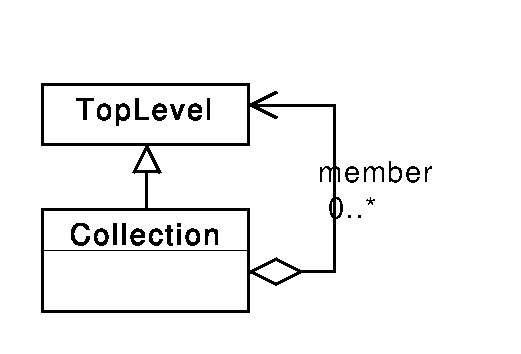
\includegraphics[scale=0.6]{uml/collection}
\caption[]{Diagram of the \sbol{Collection} class and its associated properties.}
\label{uml:collection}
\end{center}
\end{figure}

\subparagraph{The \sbolheading{member} property}\label{sec:member}
A \sbol{Collection} object can have zero or more \sbol{member} properties, each of type \sbol{IRI} specifying a \sbol{TopLevel} object.

\subsubsection{Experiment}
\label{sec:Experiment}

The purpose of the \sbol{Experiment} class is to aggregate \sbol{ExperimentalData} objects for subsequent analysis, usually in accordance with an experimental design.  Namely, the \sbol{member} properties of an \sbol{Experiment} MUST refer to \sbol{ExperimentalData} objects.




\subsection{Attachment}
\label{sec:Attachment}

\begin{figure}[ht]
\begin{center}
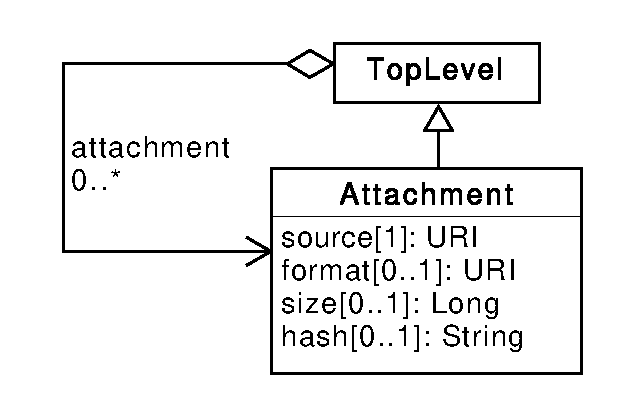
\includegraphics[scale=0.6]{uml/attachment}
\caption[]{Diagram of the \sbol{Attachment} class and its associated properties.}
\label{uml:attachment}
\end{center}
\end{figure}

The purpose of the \sbol{Attachment} class is to serve as a general container for data files, especially experimental data files.
It provides a means for linking files and metadata to SBOL designs.

The meta-data provided by the \sbol{Attachment} class include the following properties: the \sbolmult{source:A}{source} or location of the actual file of the attachment, the \sbol{format} of the file, the \sbol{size} of the file, and the \sbol{hash} for the file.

\subparagraph{The \sbolheading{source} property}\label{sec:source:A}
The \sbolmult{source:A}{source} property is REQUIRED and MUST contain a \sbol{IRI} reference to the source file.

\subparagraph{The \sbolheading{format} property}\label{sec:format}
The \sbol{format} property is OPTIONAL and MAY contain a \sbol{IRI} that specifies the format of the attached file. It is RECOMMENDED that this \sbol{IRI} refer to a term from the EMBRACE Data and Methods (EDAM) ontology.

\subparagraph{The \sbolheading{size} property}\label{sec:size}
The \sbol{size} property is OPTIONAL and MAY contain a long indicating the file size in bytes.

\subparagraph{The \sbolheading{hash} property}\label{sec:hash}
The \sbol{hash} property is OPTIONAL and MAY contain a hash value for the file contents represented as a hexadecimal digest.

\subparagraph{The \sbolheading{hashAlgorithm} property}\label{sec:hashAlgorithm}
The \sbol{hashAlgorithm} property is OPTIONAL and MAY contain the name of the hash algorithm used to generate the value of the \sbol{hash} property.
The value of this property SHOULD be a hash name string from the \href{https://www.iana.org/assignments/named-information/named-information.xhtml}{IANA Named Information Hash Algorithm Registry}, of which \texttt{sha3-256} is currently RECOMMENDED.
If the \sbol{hash} property is set, then \sbol{hashAlgorithm} MUST be set as well.


\subsection{Annotation and Extension of SBOL}
\label{sec:Annotations}

SBOL intentionally does not attempt to describe how all types of biological design data should be captured, since many of these data types (e.g., biological context and design performance metrics) are already covered by other standards, or lack a clear consensus on their proper representation, or are outside of the scope of SBOL.

SBOL is built upon the Resource Description Framework (RDF), and therefore can be used in conjunction with complementary standards as described in \ref{sec:complementaryStandards}.  For example, use of the PROV-O ontology is recommended to capture provenance (see \ref{sec:provenance}).  
Additionally, user-defined RDF can be used in conjunction with SBOL objects to capture custom application-specific information that does not yet have a standardized representation.  
This annotation and extension mechanism is designed to enable new types of data to be easily incorporated into the SBOL standard once there is community consensus on their proper representation.

Several methods are supported for connecting the SBOL data model with other types of application-specific data:

\begin{itemize}
\item Custom data can be added to an SBOL object by annotating that object with non-conflicting properties. These properties could contain \sbol{literal} data types such as \sbol{String}s or \sbol{URI}s that require a resolution mechanism to obtain external data. An example is annotating a \sbol{Component} with  a property that contains a \sbol{String} description and \sbol{URI} for the parts registry from which its source data was originally imported.
\item SBOL object classes can be extended to custom classes that add additional information. This works just like adding custom data via non-conflicting properties, except that the object receives both an \external{rdf:type} for the SBOL class that has been extended and also an \external{rdf:type} specifying the extension class.
\item Custom data in the form of independent objects can participate in the SBOL data model if they are assigned one of the SBOL types \sbol{Identified} or \sbol{TopLevel}.  An example is an RDF object that is annotated such that it represents a data sheet that describes the performance of a \sbol{Component} in a particular context.
\item Finally, just as custom objects can be embedded in an  SBOL document, external documents can embed or refer to SBOL objects. Support for this last case is not explicitly provided in this specification. Rather, this case depends on the external non-SBOL system managing its relationship to SBOL and data serialized in RDF, and is included here for completeness.
\end{itemize}

Each \sbol{Identified} object MAY be annotated with application-specific properties, which MUST be labelled using RDF predicates outside of the SBOL namespace.  Additionally, application-specific types may be used in conjunction with the SBOL data model. These application-specific types MUST have at least two \external{rdf:type} properties: one type outside of the SBOL namespace AND an additional SBOL type of either:

\begin{itemize}
  \item \sbol{TopLevel}, if the object is to be considered an SBOL top level (i.e., not owned by another object)
  \item \sbol{Identified}, if the object is not to be considered an SBOL top level (i.e., is owned by another object)
  \item The most specific applicable SBOL type, if the object is an instance of a custom class extending an SBOL class.
\end{itemize}

As with SBOL \sbol{Identified} objects, custom \sbol{Identified} objects (and thus also all other custom objects) MAY also include the properties \sbol{displayId}, \sbol{name}, \sbol{description}, etc. 


% -----------------------------------------------------------------------------
\section{Recommended Best Practices}
\label{sec:bestpractices}
% -----------------------------------------------------------------------------
\subsection{SBOL Versions}

To differentiate between major versions of SBOL, different namespaces are used.  For example, SBOL3 has the namespace \url{http://sbols.org/v3#}, while SBOL2 has the namespace \url{http://sbols.org/v2#}.  These different versions of SBOL SHOULD NOT be semantically mixed. For example, an SBOL 3.x \sbol{SubComponent} SHOULD NOT refer to an SBOL 2.x \external{ComponentInstance}, and, likewise, an SBOL 2.x \external{ComponentInstance} SHOULD NOT refer to an SBOL 1.x \external{DnaComponent}.

\subsection{Compliant SBOL Objects}
\label{sec:compliant}

Maintaining unique URIs for all SBOL objects can be challenging.  To reduce this burden, users of SBOL 3.x are encouraged to follow a few simple rules when constructing the URIs and related properties for SBOL objects.  When these rules are followed in constructing an SBOL object, we say that this object is \emph{compliant}. These rules are as follows:

Compliant URIs for \sbol{TopLevel} objects MUST conform to the following pattern:
\begin{quotation} 
\refObj{namespace}/\refObj{collection\_structure}/\refObj{displayId}
\end{quotation}

The \refObj{namespace} token MAY further decompose into \refObj{domain}/\refObj{root} tokens. The \refObj{root} and \refObj{collection\_structure} tokens may optionally be omitted; alternatively, they may consist of an arbitrary number of delimiter-separated layers. Note that this pattern means that SBOL-compliant \sbol{URI}s can be automatically decomposed with the aid of a \sbol{TopLevel} object's \sbol{hasNamespace} property. SBOL-compliant objects can be easily remapped into new namespaces by changing only the \refObj{namespace}.

Consider, for example, the SBOL-compliant \sbol{URI}:
\begin{quote}``https://synbiohub.org/igem/2017\_distribution/promoters/constitutive/BBa\_J23101''\end{quote} 
for a \sbol{Component} with a \sbol{hasNamespace} value ``https://synbiohub.org/igem/2017\_distribution''.
This \sbol{URI} can be decomposed as follows:
\begin{quote} 
namespace: ``https://synbiohub.org/igem/2017\_distribution'' \linebreak
domain: ``https://synbiohub.org'' \linebreak
root: ``igem/2017\_distribution'' \linebreak
collection: ``promoters/constitutive'' \linebreak
displayId: ``BBa\_J23101'' \linebreak
\end{quote}

SBOL-compliant URIs also facilitate auto-construction of child objects with unique \sbol{URI}s. 
Child objects of \sbol{TopLevel} objects with compliant \sbol{URI}s MUST conform to the following pattern:\\ ``\refObj{parent\_uri}/\refObj{child\_type}\refObj{child\_type\_counter}'' where the \refObj{parent\_uri} refers to the URI of the parent object, the \refObj{child\_type} refers to the SBOL class of the child object, and \refObj{child\_type\_counter} is a unique index for the child object. 
The \refObj{child\_type\_counter} of a new object SHOULD be calculated at time of object creation as 1 + the maximum \refObj{child\_type\_counter} for each \refObj{child\_type} object in the parent (e.g., ``\refObj{parent\_uri}/SequenceAnnotation37''). 
Note that numbering is independent for each type, so a \sbol{Component} can have children ``SubComponent37'' and ``Constraint37''.

All examples in this specification use compliant \sbol{URI}s.

\subsection{Versioning SBOL Objects}

SBOL 3.x does not specify an explicit versioning scheme. Rather it is left for experimentation across different tools. This allows version information to be included in the root (e.g., GitHub style: ``igem/HEAD/''), collection structure (e.g., ``promoters/constitutive/2/''), in tool-specific conventions on \sbol{displayId} (e.g., ``BBa\_J23101\_v2'') or in information outside of the \sbol{URI} (e.g., by attaching \external{prov:wasRevisionOf} properties).

\subsection{Annotations: Embedded Objects vs. External References}

When annotating an SBOL document with additional information, there are
two general methods that can be used:
\begin{itemize}
\item Embed the information in the SBOL document using properties outside of the SBOL namespace.
\item Store the information separately and annotate the SBOL document with \sbol{URI}s that point to it.
\end{itemize}
In theory, either method can be used in any case. (Note that a third case not
discussed here is to annotate external objects with links
to SBOL documents, rather than annotating SBOL documents with links to external objects.)

In practice, 
embedding large amounts of non-SBOL data into SBOL documents is likely
to cause problems for people and software tools trying to manage and
exchange such documents.  Therefore, it is RECOMMENDED that small amounts of information (e.g., design notes or preferred graphical layout) be embedded in the SBOL model, while large amounts of information (e.g., the contents of the scientific publication from which a model was derived or flow cytometry data that characterizes performance) be linked with URIs pointing to external resources.  The boundary between ``small'' and ``large'' is left deliberately vague, recognizing that it will likely depend on the particulars of a given SBOL application.

\subsection{Completeness and Validation}

RDF documents containing serialized SBOL objects might or might not be
entirely self-contained.  A SBOL document is self-contained or ``complete'' if every SBOL object referred to in the document is contained in the document.  It is RECOMMENDED that serializations be complete whenever practical.  In order words, when serializing an SBOL object, serialize all of the other objects that it points to, then serialize all of the other objects that these objects point to, etc., until the document is complete.

It is important to note that there is no guarantee that an RDF document
contains valid SBOL. When SBOL objects are read from an RDF document,
 the program doing so SHOULD verify that all of the property
values encoded therein have the correct data type (e.g., that the object
pointed to by the \sbol{Sequence} property of a
\sbol{Component} is really a \sbol{Sequence}).
For complete files, this validation can be carried out entirely locally. For files that are not complete, an implementation either needs to have a means of validating those external references (e.g., by
retrieving them from a repository), or it needs to mark them as
unverified and not depend on their correctness.

\subsection{Recommended Ontologies for External Terms}
\label{sec:recomm_ontologies}

External ontologies and controlled vocabularies are an integral part of SBOL. SBOL uses \sbol{URI}s to access existing biological information through these resources. 
New SBOL-specific terms are defined only when necessary. 
For example, \sbol{Component} \sbolmult{type:C}{type}s, such as DNA or protein, are described using Systems Biology Ontology (SBO) terms. Similarly, the \sbolmult{role:C}{role}s of a DNA or RNA \sbol{Component} are described via Sequence Ontology (SO) terms. Although RECOMMENDED ontologies have been indicated in relevant sections where possible, other resources providing similar terms can also be used. A summary of these external sources can be found in \ref{tbl:preferred_external_resources}.

\begin{table}[htp]
  \begin{edtable}{tabular}{p{2cm}p{1.5cm}p{5cm}p{6cm}}
    \toprule
    \textbf{SBOL Entity} & \textbf{Property} & \textbf{Preferred External Resource}
    & \textbf{More Information} \\
    \midrule
    \textbf{Component}  & type & SBO (physical entity branch)& \url{http://www.ebi.ac.uk/sbo/main/}\\
                                  & type & SO (nucleic acid topology)& \url{http://www.sequenceontology.org}\\
    						   	  & role & SO (\textit{DNA} or \textit{RNA}) & \url{http://www.sequenceontology.org}   \\
    						   	  & role & CHEBI (\textit{small molecule}) & \url{https://www.ebi.ac.uk/chebi/}   \\
							  & role & PubChem (\textit{small molecule}) & \url{https://pubchem.ncbi.nlm.nih.gov/} \\
    						   	  & role & UniProt (\textit{protein}) & \url{https://www.uniprot.org/}  \\   
    						   	  & role & NCIT (\textit{samples}) & \url{https://ncithesaurus.nci.nih.gov/}  \\   
    \textbf{Interaction}	      & type & SBO (occurring entity branch) & 
    \url{http://www.ebi.ac.uk/sbo/main/} \\
    \textbf{Participation}	      & role & SBO (participant roles branch) &
    \url{http://www.ebi.ac.uk/sbo/main/} \\
    \textbf{Model}	      		  & language & EDAM & \url{http://bioportal.bioontology.org/ontologies/EDAM}     \\
    				      		  & framework & SBO (modeling framework branch) &
    \url{http://www.ebi.ac.uk/sbo/main/} \\
    \textbf{om:Measure}	& type & SBO (systems description parameters) &
    \url{http://www.ebi.ac.uk/sbo/main/} \\
    \bottomrule
  \end{edtable}
  \caption{Preferred external resources from which to draw values for various SBOL properties.}
  \label{tbl:preferred_external_resources}
\end{table}

The URIs for ontological terms SHOULD come from identifiers.org.  However, it is acceptable to use terms from purl.org as an alternative, for example when RDF tooling requires URIs to be represented as compliant QNames.  SBOL software may convert between these forms as required.

\subsection{Annotating Entities with Date \& Time}\label{sec:DateTime}

Entities in an SBOL document can be annotated with creation and modification dates. It is RECOMMENDED that predicates, or properties, from DCMI Metadata Terms SHOULD be used to include date and time information. The \texttt{created} and \texttt{modified} terms SHOULD respectively be used to annotate SBOL entities with creation and modification dates. Date and time values SHOULD be expressed using the XML Schema \texttt{DateTime} datatype~\citep{Biron2004}. For example, ``\texttt{2016-03-16T20:12:00Z}'' specifies that the day is 16 March 2016 and the time is 20:12pm in UTC (Coordinated Universal Time).

\subsection{Annotating Entities with Authorship information}\label{sec:Authorship}

Authorship information should ideally be added to \sbol{TopLevel} entities where possible. It is RECOMMENDED that the \texttt{creator} DCMI Metadata term SHOULD be used to annotate SBOL entities with authorship information using free text. This property can be repeated for each author.
%The example below shows the use of this property for two authors and the values shown are free text \texttt{String} literals.

\subsection{Host Context / Ontologies for Experiments}

\subsubsection{Mixtures via Components}

Any \sbol{Component} can be interpreted as specifying a mixture of the material entity (SBO:0000240) \sbol{Feature}s that it includes.  The amount of each such instance included in the mixture SHOULD be specified by attaching a \om{Measure} with a \sbolmult{type:Measure}{type} set to the appropriate SBO term. The SBO terms that are RECOMMENDED as appropriate are members of the Systems Description Parameter (SBO:0000545) branch of SBO. Examples include:
\begin{itemize}
\item SBO:0000540: fraction of an entity pool (e.g., 1/3 CHO cells, 2/3 HEK cells)
\item SBO:0000472: molar concentration of an entity (e.g., 1 mM arabinose)
\item SBO:0000361: amount of an entity pool (e.g., 200 uL M9 media)
\end{itemize}

Mixtures MAY be defined recursively, as mixtures of mixtures of mixtures, etc.

\subsubsection{Media, Inducers, and Other Reagents}

Each reagent, whether ``atomic'' (e.g., rainbow bead control) or mixture (e.g., M9 media), SHOULD be represented as a \sbol{Component} and/or as a \sbol{Feature} of a \sbol{Component} in which the reagent is used.
For example, a custom media mixture might be defined as a \sbol{Component} and used as a \sbol{SubComponent}, while a commercially supplied reagent might be used as an \sbol{ExternallyDefined} feature linking to its PubChem identifiers.

The roles of reagents may vary in context: for example, arabinose may serve as an inducer or as a media carbon source. As such, contextual role SHOULD be indicated by an NCI Thesaurus (NCIT) term in a \sbolmult{role:F}{role} property of the \sbol{Feature}. Examples include:
\begin{itemize}
\item NCIT:C64356: Positive Control
\item NCIT:C48694: Cell
\item NCIT:C85504: Media
\item NCIT:C14419: Strain
\item NCIT:C120268: Inducer
\end{itemize}

For more information on representing cells, strains, plasmids, and genomes, see \ref{bp:cells}

%\todo[inline]{Should we switch the GO term recommendation below to match the NCIT recommendation below?}

\subsubsection{Samples}

A complete specification of a sample SHOULD be a \sbol{Component} that includes at least:
\begin{itemize}
\item A \sbol{Feature} instantiating each strain in the sample
\item A \sbol{Feature} for the media or buffer
\item A \sbol{Feature} for each additional reagent added to the media (e.g., inducers, antibiotics)
\item \om{Measure}s on each of these specifying the amount in the sample
\item \om{Measure}s on the \sbol{Component} for each environmental parameter (e.g., temperature, pH, culturing time)
\end{itemize}

\subsubsection{Other Experimental Parameters}

In order to deal with parameters associated with the context in general but not specific instances, e.g., temperature, pH, total sample volume, the \sbol{hasMeasure} property of \sbol{Identified} can be used.  The \sbol{hasMeasure} of a \sbol{Component} provides context-free information (e.g., the pH of M9 media, the GC-content of a GFP coding sequence), while the \sbol{hasMeasure} of a material entity (SBO:0000240) \sbol{Feature} provides a measurement in context (e.g., the dosage of arabinose in a sample).

Values of these parameters SHOULD be specified by attaching a \om{Measure} with a \sbolmult{type:Measure}{type} set to the appropriate SBO term. The SBO terms that are RECOMMENDED as appropriate are members of the Systems Description Parameter (SBO:0000545) branch of SBO. Examples include:
\begin{itemize}
\item SBO:0000147: thermodynamic temperature (e.g., culturing at 27 C)
\item SBO:0000332: half-life of an exponential decay (e.g., decay rate of a gRNA)
\item SBO:0000304: pH (e.g., pH of M9 media)
\end{itemize}


\subsection{Multicellular System Designs}

SBOL has been used extensively to represent designs in homogeneous systems, where the same design is implemented in every cell. However, in recent years there has been increasing interest in multicellular systems, where biological designs are split across multiple cells to optimize the system behavior and function. Therefore, there is a need to define a set of best practices so that multicellular systems can be captured using SBOL in a standard way.

\subsubsection{Representing Cell Types}
\label{bp:cells}

To represent multicellular systems using SBOL, it is first necessary to represent cells. 
When doing so, it is important to be able to capture the following information: (i) taxonomy of the strain used, (ii) interactions occurring within cells of this type, and (iii) components inside the type of cell (e.g. genomes, plasmids). 
The approach RECOMMENDED in this section is capable of capturing this information, as shown in the example in \ref{uml:cell_representation}. 
It uses a \sbol{Component} to represent a system that contains cells of the given type.
The cells themselves are represented by a \sbol{Feature} inside the \sbol{Component}, in this case a \sbol{SubComponent} that is an \sbol{instanceOf} 
a \sbol{Component} capturing information about the species and strain of the cell in the design. 
This \sbol{Component} has a \sbolmult{type:C}{type} of ``cell'' from the Cell Ontology (CL:0000000), and a \sbolmult{role:C}{role} of ``physical compartment'' (SBO:0000290).
%\todo[inline]{What property are we actually recommending to use for the annotation?}
Taxonomic information is captured by annotating the class instance with a URI for an entry in the NCBI Taxonomy Database. 

As usual, other entities besides the cell that are relevant to the design are also captured as \sbol{Feature}s.
When these are contained within the cell, they are captured using a \sbol{Constraint} with restriction \texttt{contains} with the cell as \sbol{subject} and contained object as \sbol{object}.
Interactions which occur in this system are captured using the \sbol{Interaction} and \sbol{Participation} classes. 
Interactions which occur within the cell are specified by \sbol{Interaction} classes which contain the \sbol{Feature} instance representing the cell as a \sbol{participant} with a \sbolmult{role:P}{role} of ``physical compartment'' (SBO:0000290).

\begin{figure}[htp]
	\begin{center}
		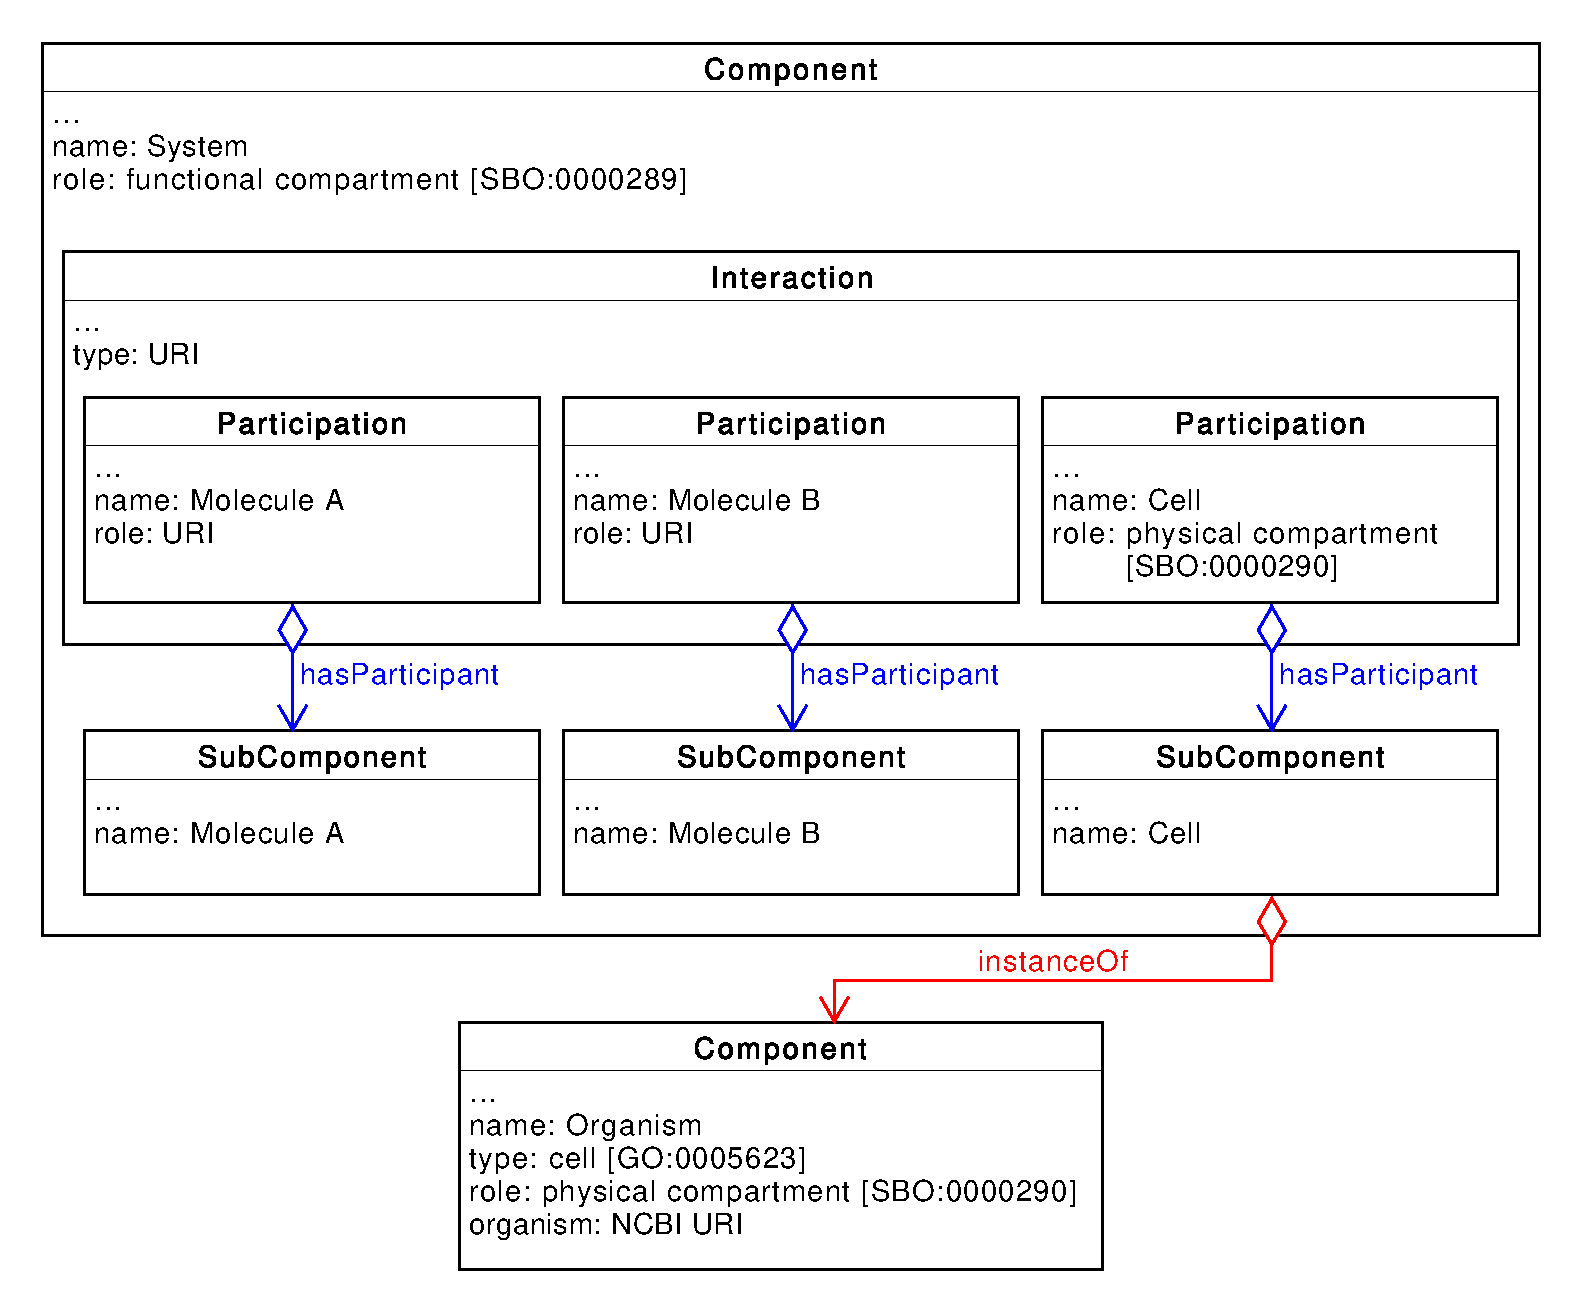
\includegraphics[width=\textwidth]{uml/cell_representation}
		\caption[Repressenting a cell]{This is a proposed approach for capturing cell designs in SBOL. A \sbol{Component} annotated with a URI pointing to an entry in the NCBI Taxonomy Database is used to capture information about the cell's strain/species. 
		The \sbol{Component} has a type of ``Cell'' from the Gene Ontology (GO), and a role of ``physical compartment''. 
		Another \sbol{Component} is used to represent a system in which the cell is implemented. 
		Entities, including the cell, are instantiated as \sbol{Feature}s, and processes are captured using the \sbol{Interaction} class.
		Processes that are contained within the cell are represented by including the cell as a participant with a role of ``physical compartment''. }
		\label{uml:cell_representation}
	\end{center}
\end{figure}

\subsubsection{Multiple Cell Types in a Single Design}

The same approach can be extended to represent systems with multiple types of cells.
The multicellular system can be represented as a \sbol{Component} that includes each strain of cell as a \sbol{Feature}, in this example a \sbol{SubComponent} that is an \sbol{instanceOf} a \sbol{Component} defining its strain.
Interactions and constraints, such as a molecule that both strains interact with, are implemented using \sbol{ComponentReference}s to link to the definitions within each cell system description.
An example is shown in \ref{uml:multiple_cell_representation}.

\begin{figure}[htp]
	\begin{center}
		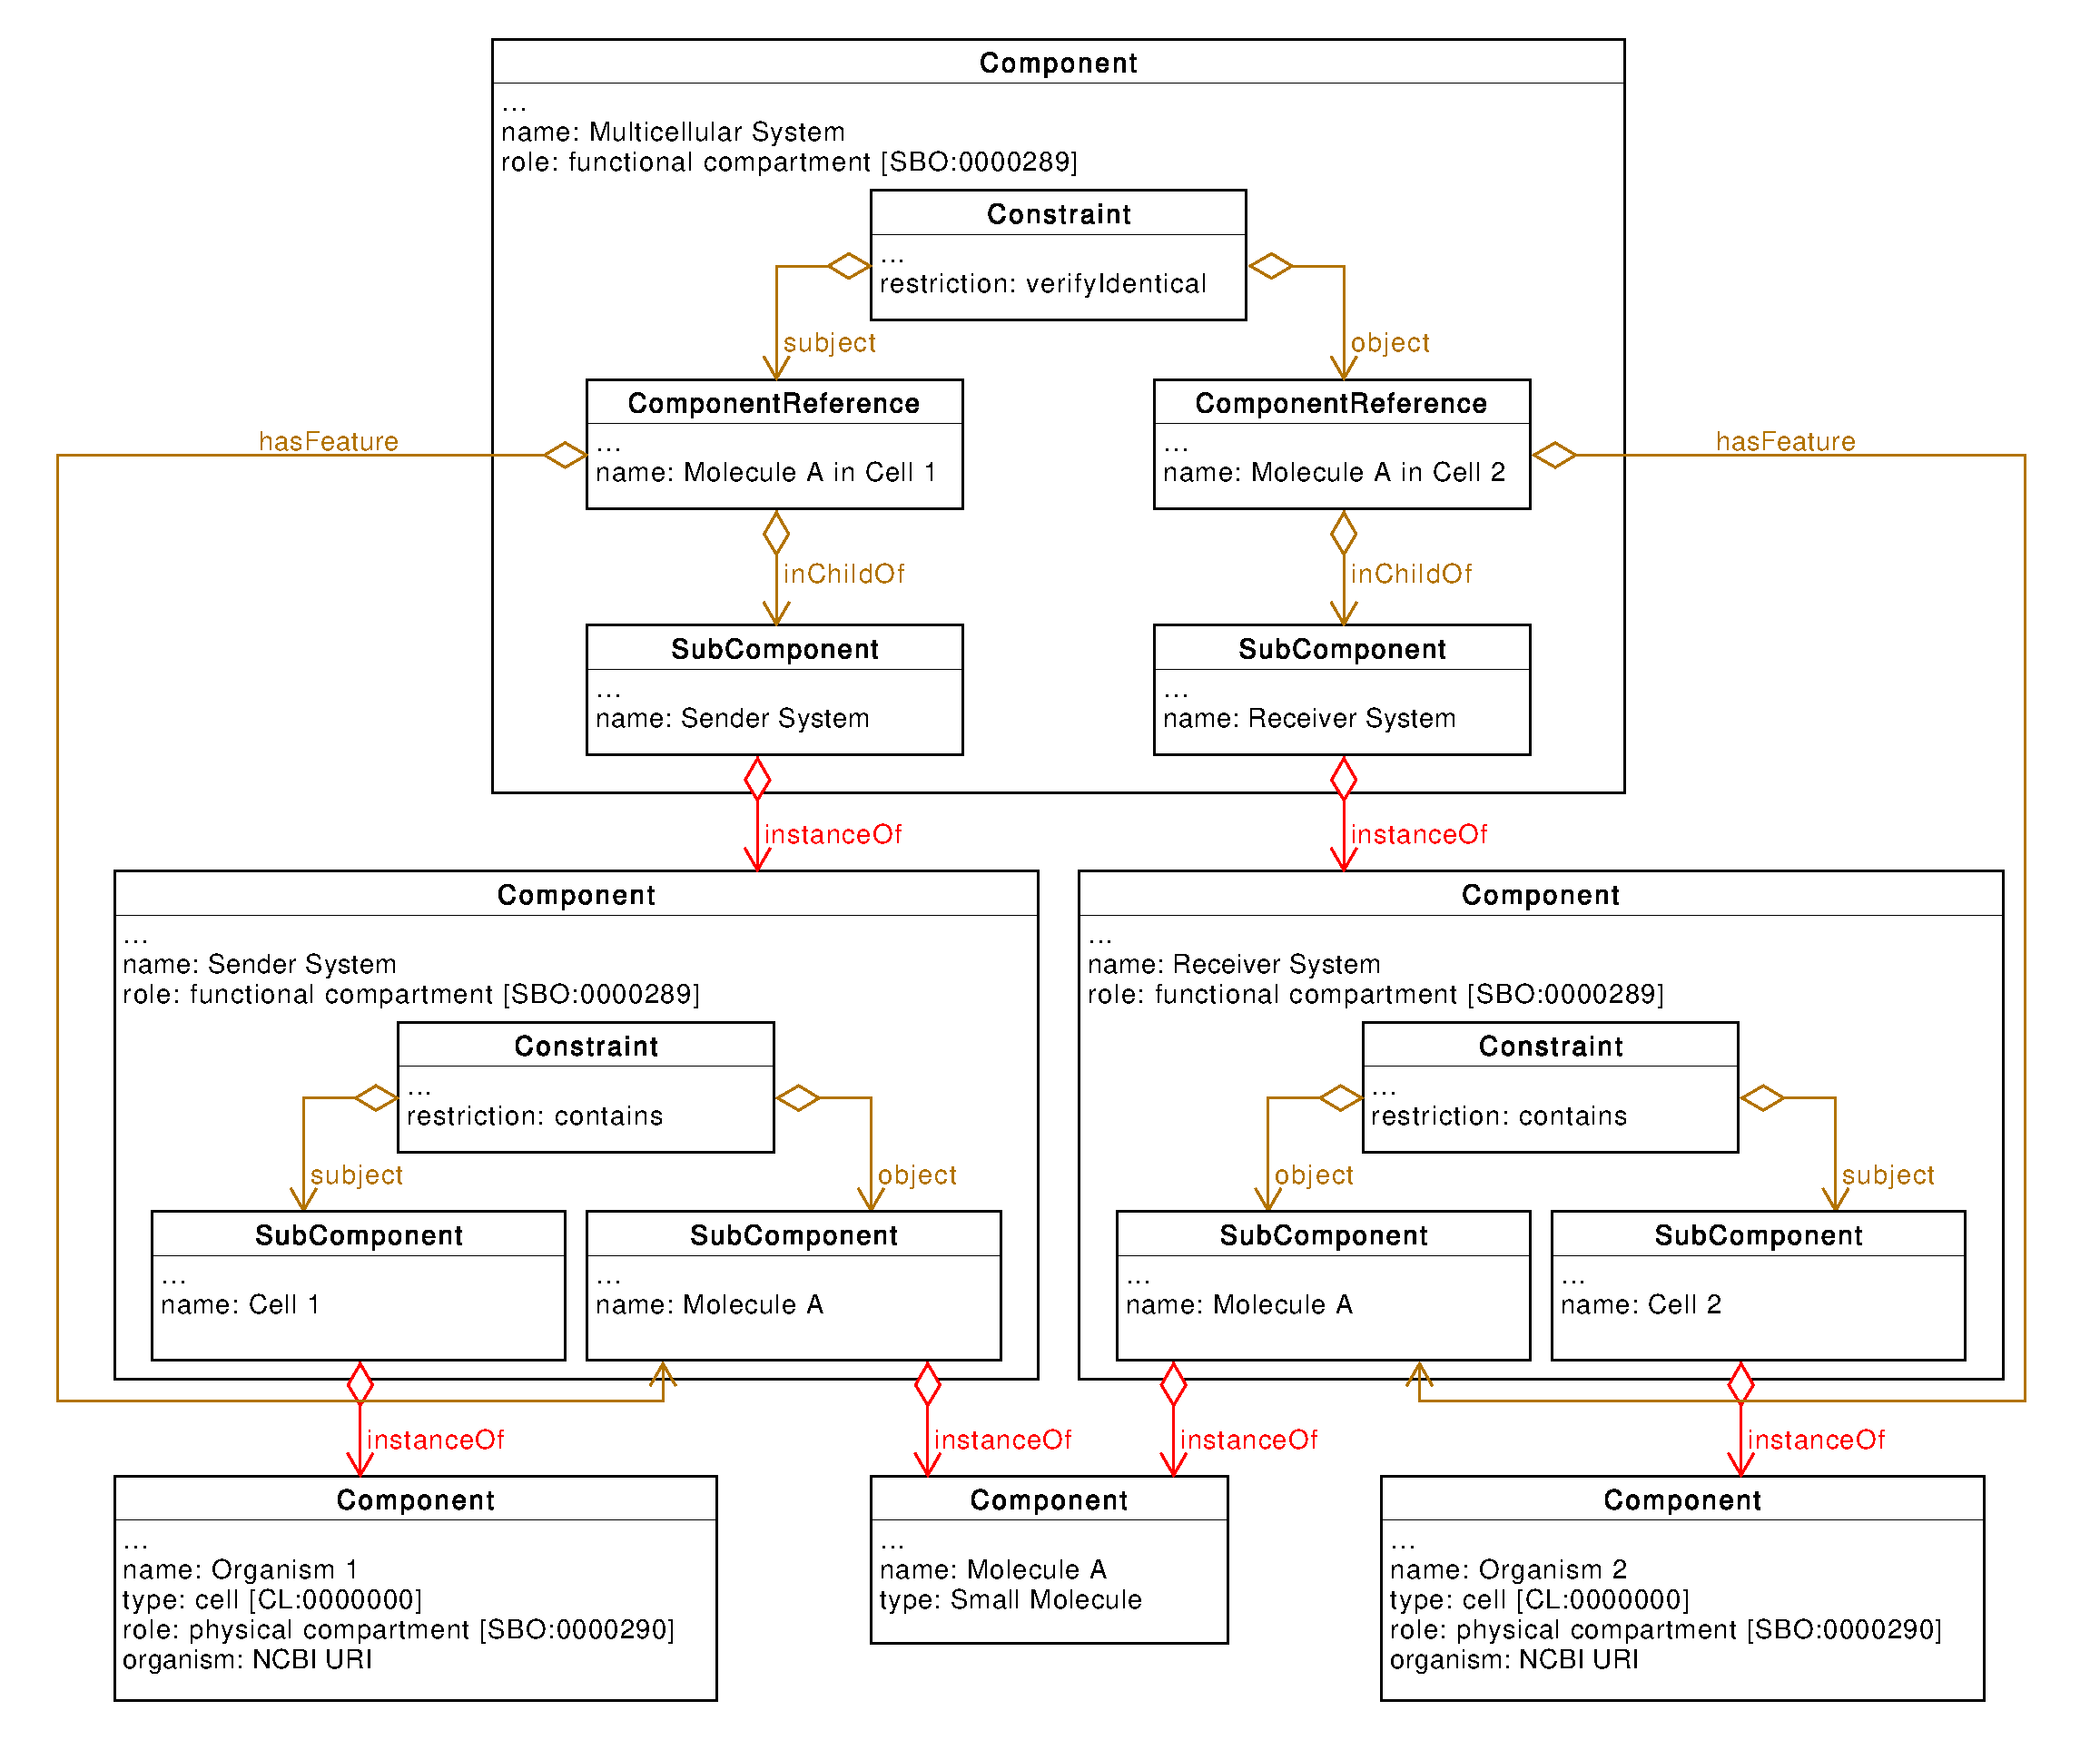
\includegraphics[width=\textwidth]{uml/two_cell_representation}
		\caption[]{Captured here is a design involving two cells which both interact with the small molecule ``Molecule A''. 
		Designs for the sender and receiver systems are captured using constraint to show that each of these cells interacts with the Molecule A contained within it.
		The overall multicellular system is represented by a \sbol{Component} with a \sbolmult{role:C}{role} of ``functional compartment'', which is an SBO term.
		The two systems are included in this multicellular design as \sbol{Feature}s, and the fact that Molecule A is shared between systems is indicated with a constraint.}
		\label{uml:multiple_cell_representation}
	\end{center}
\end{figure}

\subsubsection{Cell Ratios}

The proportion of cell types present in a multicellular system can be captured using \om{Measure} on the representations of cells in the design.
As a best practice, the value of these measure classes is a percentage less than or equal to 100\%, representing the amount of a cell type present in the system compared to all other cell types present. 
Therefore, the sum of all these values specified in the system will typically be equal to 100\%, though this may not be the case if the system is not completely defined. 
An example is shown in \ref{uml:cell_ratios}.

\begin{figure}[htp]
	\begin{center}
		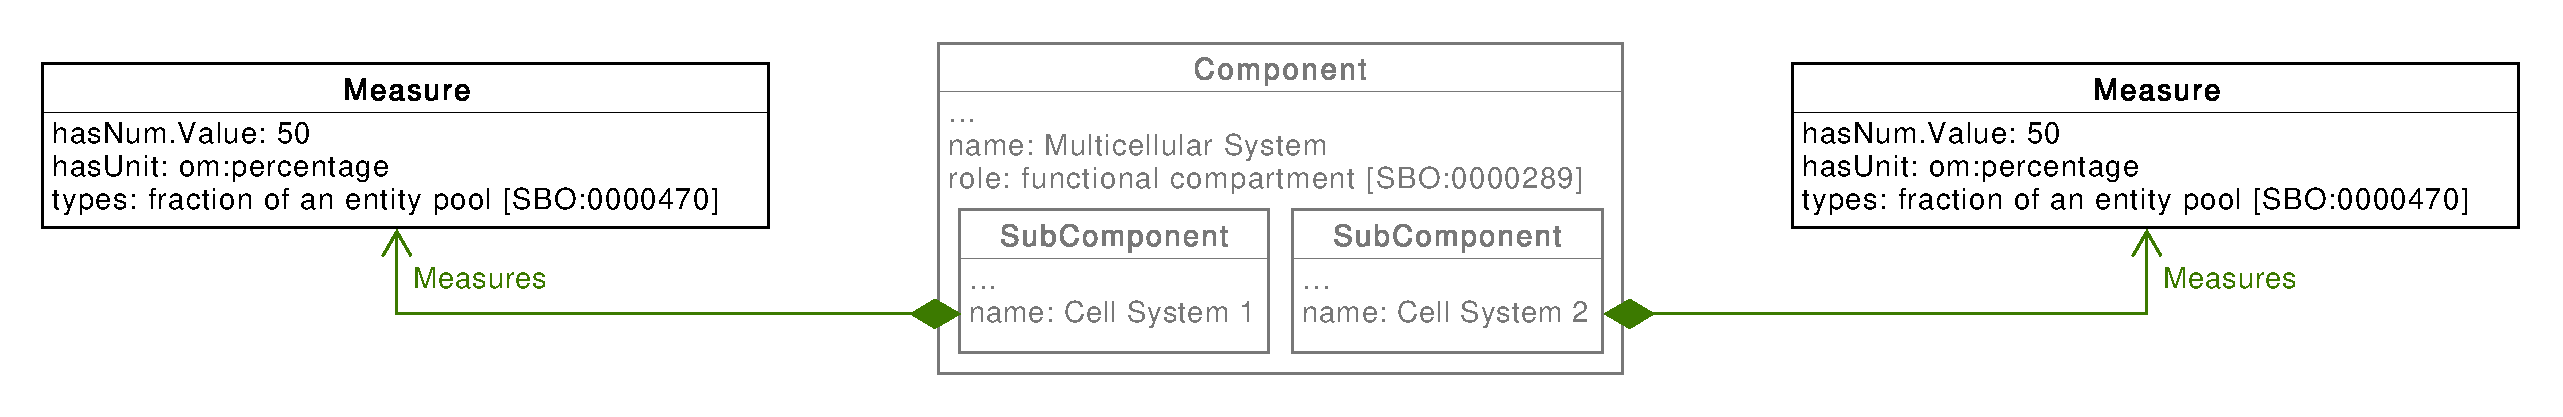
\includegraphics[width=\textwidth]{uml/cell_ratios}
		\caption[]{Annotating class instances with cellular proportions. Instances of the Measure class are used to capture the percentage of each cell type present in the multicellular system design.
		}
		\label{uml:cell_ratios}
	\end{center}
\end{figure}


% % -----------------------------------------------------------------------------
\section{Data Model Examples}
\label{sec:examples}
% -----------------------------------------------------------------------------

%\subsection{LacI/TetR Toggle Switch}

This section illustrates how to use the SBOL data model by specifying the design of a LacI/TetR toggle switch similar to those constructed in \cite{Gardner2000}. This design is visualized conceptually in \ref{images:toggle} and in detail in \ref{images:toggleswitch_modular}. 

Conceptually, the toggle switch is constructed from two mutually repressing genes.  
With repressors LacI and TetR, this results in a bi-stable system that will tend to settle into a state where precisely one of the two repressors is strongly expressed, repressing the other.
Each of these repressors can have its activity disrupted by a small molecule (IPTG for LacI, aTc for TetR), which enables the system to be ``toggled'' from one state to the other by dosing it with the appropriate small molecule.


\begin{figure}[ht]
\begin{center}
\includegraphics[width=0.33\textwidth]{images/toggle-highlevel2.pdf}
\caption[]{Conceptual diagram of LacI/TetR toggle switch: the LacI 
  and TetR transcription factors are arranged to mutually repress each other's expression, 
  creating a bi-stable system.  Transition between the two states
  is triggered by the small-molecule signals aTc (which disrupts TetR
  repression) and IPTG (which disrupts LacI repression).}
\label{images:toggle}
\end{center}
\end{figure}

\begin{figure}[ht]
\begin{center}
\includegraphics[width=\textwidth]{images/toggleswitch_modular2}
\caption[]{Design of a LacI/TetR toggle switch. This design is composed of two inverter sub-designs, each containing a single gene. These genes mutually repress each other's expression via their encoded protein transcription factors, LacI and TetR. Furthermore, both LacI and TetR are bound by specific small molecules that sequester them and prevent them from acting as repressors. In this design, arrows represent different molecular interactions, including the repression of pLac via LacI, the non-covalent binding of IPTG to LacI, the transcription of TetR mRNA, and the translation of TetR. Dashed lines serve to map between transcription factors in the inverter sub-designs and those in the overall toggle switch design.}
\label{images:toggleswitch_modular}
\end{center}
\end{figure}


The LacI/TetR toggle switch is modeled in SBOL as two parallel hierarchies of structure and function. The structural hierarchy of the toggle switch is represented using \sbol{Component}s:
\begin{itemize}
\item The base elements of the hierarchy are DNA components, transcription factor proteins, and small molecules. As an example, \ref{uml:ex_comp_defs} is a UML diagram of the \sbol{Component} objects that represent these elements.
\item Base elements are composed to form more complex structures at the top of the hierarchy, including genes and non-covalent complexes between transcription factor proteins and small molecules. As an example, \ref{uml:ex_comp_def_compo} is a UML diagram of the composite \sbol{Component} objects that represent the TetR gene and IPTG-LacI complex.
\end{itemize}

\begin{figure}[ht]
\begin{center}
\includegraphics[width=\textwidth]{example_uml/toggle_1}
\caption[]{\sbol{Component} objects for the LacI inverter. These include \sbol{Component} objects based on DNA parts from the iGEM Parts Registry and  \sbol{Component} objects that represent TetR mRNA, TetR, LacI, and IPTG. Each \sbol{Component} is associated with a \sbol{Sequence} that has an \external{IUPAC DNA/RNA} or \external{IUPAC protein} \sbol{encoding}, except the \sbol{Component} of IPTG, which is associated with a \sbol{Sequence} that has a \external{SMILES} \sbol{encoding}.}
\label{uml:ex_comp_defs}
\end{center}
\end{figure}


\begin{figure}[ht]
\begin{center}
\includegraphics[width=\textwidth]{example_uml/toggle_2}
\caption[]{Composite \sbol{Component} objects for the LacI inverter. In the case of the \sbol{Component} that represents the TetR gene, its sub-\sbol{SubComponent} objects are located as \sbol{Range}s along its \sbol{Sequence} using \sbol{SequenceFeature} objects. The \sbol{Component} that represents the IPTG-LacI complex, however, has no \sbol{Sequence} and its sub-\sbol{SubComponent} objects are composed without any data about their relative positions.}
\label{uml:ex_comp_def_compo}
\end{center}
\end{figure}
\todo{Change SequenceAnnotations to SequenceFeatures}

The functional hierarchy of the toggle switch is represented using
\sbol{Component}s:
\begin{itemize}
\item The base elements of the hierarchy are LacI-dependent repression of TetR expression (the LacI inverter) and TetR-dependent repression of LacI (the TetR inverter). As an example, \ref{uml:ex_mod_def} is a UML diagram of the \sbol{Component} that represents the LacI inverter.
\item Base elements are composed to form the toggle switch at the top of the hierarchy.  As an example, \ref{uml:ex_mod_def_compo} is a UML diagram of the \sbol{Component} that represents the toggle switch.
\end{itemize}

\begin{figure}[ht]
\begin{center}
\includegraphics[width=\textwidth]{example_uml/toggle_3}
\caption[]{\sbol{Component} of the LacI inverter. This \sbol{Component} contains \sbol{SubComponent} objects that instantiate the \sbol{Component} objects for the LacI/TetR transcription factors and TetR gene. These \sbol{SubComponent} objects participate in a repression \sbol{Interaction} and a genetic production \sbol{Interaction}, thereby indicating which biological structures carry out the function of the LacI inverter \sbol{Component}. In this case, the transcription and translation of TetR are represented as a single genetic production \sbol{Interaction} that abstracts away the presence of the intermediate TetR mRNA.  In addition, this \sbol{Component} is also associated with a continuous \sbol{Model} written in the SBML source file ``LacI\_Inverter.xml.''}
\label{uml:ex_mod_def}
\end{center}
\end{figure}

\begin{figure}[ht]
\begin{center}
\includegraphics[width=\textwidth]{example_uml/toggle_4}
\caption[]{Composite \sbol{Component} of the LacI/TetR toggle switch. This \sbol{Component} contains the \sbol{SubComponent} objects that instantiate LacI and TetR inverter \sbol{Component} objects. It also contains \sbol{SubComponent} objects that instantiate the \sbol{Component} objects for the LacI/TetR transcription factors and IPTG/aTc small molecules. These \sbol{SubComponent} objects each participate in a non-covalent binding \sbol{Interaction}. To complete the composition of the toggle switch, \sbol{MapsTo} objects are used to indicate that the output of the LacI inverter \sbol{Component} is identical to the input of the TetR inverter \sbol{Component} and vice versa.}
\label{uml:ex_mod_def_compo}
\end{center}
\end{figure}

\todo[inline]{revise figure 29! No MapsTos}

% Each \sbol{Component} also contains the \sbol{SubComponent}s that participate in \sbol{Interaction}s and are defined by the same \sbol{Component}s as the parallel \sbol{SubComponent}s in the structural hierarchy of the toggle switch. Finally, \sbol{MapsTo} entities are used to refine which \sbol{SubComponent}s of the functional hierarchy are identical or map them to \sbol{SubComponent}s in the structural hierarchy.

%  The first use case is to indicate with greater fidelity how a module describes the function of a composite component, namely by asserting that particular component instantiations within the module correspond to particular component instantiations within the component. 

% As an example of this use case, one might compose the structure and function of the LacI-repressible gene of the genetic toggle switch. In this example, the LacI-repressible gene and two of its subcomponents, the pLac promoter and cTetR CDS, are to be composed with the LacI inverter module. In order to compose these components with the LacI inverter module and indicate that it describes their behavior, they are instantiated inside the module. In addition, port maps are placed on the instantiation of the LacI-repressible gene to connect between its pLac plus cTetR subcomponent instantiations and the corresponding component instantiations in the module. Doing so makes it clear which subcomponent instantiations in the gene are being described by which component instantiations in the module. In this way, GDA tools for sequence editing and biochemical modeling can guarantee that their users are handling corresponding elements of a given genetic design, while GDA tools for genetic technology mapping can make explicit connections between the structural and functional elements of a design.


% -----------------------------------------------------------------------------
\section{SBOL RDF Serialization}
\label{sec:serialization}
% -----------------------------------------------------------------------------

In order for SBOL objects to be readily stored and exchanged, it is important that they are able to be {\em serialized}, i.e., converted to a sequence of bytes that can be stored in a file or exchanged over a network.  The serialization format for SBOL is designed to meet several competing requirements. 
First, SBOL needs to support ad-hoc annotations and extensions. 
Second, SBOL needs to support processing by general database and semantic web software tools that have little or no knowledge of the SBOL data model. 
Finally, it ought to be relatively simple to write a new software implementation, so that SBOL can be readily used even in software environments where community-maintained implementations are not available.

To meet these goals, SBOL builds upon the Resource Description Framework (RDF).  RDF is an abstract language for describing conceptual graph-oriented data models, and therefore does not mandate any specific serialization format.  Instead, a number of different serialization formats are provided as separate specifications, such as RDF/XML, N-Triples, JSON-LD, and Turtle.  These serialization formats are widely supported by RDF libraries such as rdflib for Python and Apache Jena for Java.   For example, a simple SBOL definition of pLac can be serialized in RDF/XML as follows:

\vspace{3mm}
\includegraphics{example_serialization/example_rdfxml.pdf}

Alternatively, the same example can be serialized in Turtle as follows:

\vspace{3mm}
\includegraphics{example_serialization/example_turtle.pdf}

The SBOL namespace, which is \url{http://sbols.org/v3\#}, is used to indicate which entities and properties in the SBOL document are defined by SBOL. For example, the URI of the type \sbol{Component} is \url{http://sbols.org/v3\#Component}. The SBOL namespace MUST NOT be used for any entities or properties not defined in this specification.  Where possible, we have re-used predicates from widely-used terminologies (such as Dublin Core~\cite{dcmi2012}) to expose as much of the data as practical to such standard RDF tooling.



\section{SBOL Compliance}

There are different types of software compliance with respect to the SBOL specification.  First, a software tool can either support all classes of the SBOL 3 data model or only its structural subset.  The structural subset includes the following classes:
\begin{itemize}
\item \sbol{Sequence}
\item \sbol{Component}
\begin{itemize}
\item \sbol{SubComponent}
\item \sbol{ComponentReference}
\item \sbol{LocalSubComponent}
\item \sbol{SequenceFeature}
\item \sbol{Location}
\item \sbol{Constraint}
\end{itemize}
\item \sbol{Collection}
\end{itemize}
Second, an SBOL-compliant software tool can support import of SBOL, export of SBOL, or both.  
If it supports both import and export, it can do so in either a lossy or lossless fashion.

In order to test import compliance, developers are encouraged to use the SBOL test files found here:\\ {\url{https://github.com/SynBioDex/SBOLTestSuite}}\\
Examples of every meaningful subset of objects are provided, including both structural-only SBOL (that is, annotated DNA sequence data) and complete tests.  

In order to test export compliance, developers are encouraged to validate SBOL files generated by their software with the SBOL Validator found here:\\
\url{https://validator.sbolstandard.org}\\
This validator can also be used to check lossless import/export support, since it can compare the data content of files imported and exported by a software tool.

Finally, developers of SBOL-compliant tools are encouraged to notify the SBOL editors\\(sbol-editors@googlegroups.com) when they have determined that their tool is SBOL compliant, so their tool can be publicly categorized as such on the SBOL website.




\section{Mapping Between SBOL 1, SBOL 2, and SBOL3}
\label{sec:mapping}

In broad strokes, the SBOL 1 standard focused on conveying physical, structural information, whereas SBOL 2 expanded the scope to include functional aspects as well.  
The physical information about a designed genetic construct includes the order of its constituents and their descriptions. 
Specifying the exact locations of these constituents and their sequences allows genetic constructs to be defined unambiguously and reused in other designs. 
SBOL 2 extended SBOL 1 in several ways: it extends physical descriptions to include entities beyond DNA sequences, and it added support for functional descriptions of designs.  
SBOL 3 refines the SBOL 2 data model to simplify the representation of common use cases.

\subsection{Mapping between SBOL 1 and SBOL 2}

\ref{SBOL1TO2} depicts the mapping of SBOL 1.1 classes to SBOL 2.x classes, indicating corresponding classes/properties by color.
The SBOL 2.x \external{Model} and \external{ModuleDefinition} classes have no SBOL 1.1 equivalent, and thus are not shown.
The mapping from SBOL 1.1 to SBOL 2.x proceeds as follows:
\begin{itemize}
\item SBOL 1.1 \external{Collection} objects containing \external{DnaComponent} objects map to SBOL 2.x \external{Collection} objects that contain \external{CompenentDefinition} objects with DNA \sbolmult{type:C}{type} properties.
\item SBOL 1.1 \external{DnaComponent} objects map to SBOL 2.x \external{CompenentDefinition} objects with DNA \sbolmult{type:C}{type} properties.
\item SBOL 1.1 \external{DnaSequence} objects map to an SBOL 2.x \external{Sequence} objects with \external{IUPAC DNA} \external{encoding} properties.
\item SBOL 1.1 \external{SequenceAnnotation} objects with \external{bioStart} and \external{bioEnd} properties map to SBOL 2.x\\
\external{SequenceAnnotation} objects that contain \external{Range} objects.
\item SBOL 1.1 \external{SequenceAnnotation} objects that lack \external{bioStart} and \external{bioEnd} properties map to an SBOL 2.x \external{SequenceFeature} objects that contain \external{GenericLocation} objects.
\item Each SBOL 1.1 \external{SequenceAnnotation} also maps to an SBOL 2.x \external{Component}, which represents the instantiation or usage of the appropriate \external{CompenentDefinition}.
\item Each SBOL 1.1 \external{precedes} property maps to an SBOL 2.x \external{SequenceConstraint} that specifies a \external{precedes} \external{restriction} property.
\end{itemize}

\begin{figure*}[htp]
\begin{center}
  \includegraphics[width=0.95\textwidth]{images/sbol_v1_to_v2}
\end{center}
\caption{\label{SBOL1TO2}The mapping from the SBOL 1.1 data model to the SBOL 2.x  data model, indicating corresponding classes/properties by color.}
\end{figure*}



\subsection{Mapping between SBOL 2 and SBOL 3}

\ref{SBOL2TO3} depicts the mapping of SBOL 2.3 classes to SBOL 3.x classes, indicating corresponding classes/properties by color.   
The SBOL 3.x \sbol{Namespace} class has no SBOL 2.x equivalent, and thus is not shown.
The SBOL 2.x \sbol{Attachment}, \sbol{CombinatorialDerivation}, \sbol{ExperimentalData}, \sbol{Experiment}, \sbol{Implementation}, \sbol{Model}, \sbol{Participation}, \\
\sbol{Sequence}, and \sbol{VariableComponent} classes are omitted or abstracted, since they are essentially unchanged in SBOL 3.x except for the following property renamings:
\begin{itemize}
\item In \sbol{Sequence}, the \sbol{encoding} property values for IUPAC map according to  \ref{tbl:sequence_encoding_mapping}. 
\item In \sbol{VariableComponent}, the SBOL 2.x \external{operator} property maps to the SBOL 3.x \sbol{cardinality} property.
\item In \sbol{Experiment}, the SBOL 2.x \external{experimentalData} property maps to the SBOL 3.x \sbol{member} property.
\end{itemize}

The mapping from SBOL 2.x to SBOL 3.x proceeds as follows:
\begin{itemize}
    \item SBOL 2.x \external{ComponentDefinition} objects map to SBOL 3.x \sbol{Component} objects.  The \sbolmult{type:C}{type} property is mapped according to  \ref{tbl:component_type_mapping}.
    \item SBOL 2.x \external{ModuleDefinition} objects map to SBOL 3.x \sbol{Component} objects with a \sbolmult{type:C}{type} of \texttt{SBO:0000241} (functional entity)
    \item Every \external{FunctionalComponent} in an SBOL 2.x \external{ModuleDefinition} with a "direction" property that is not "none" is listed in the \sbol{Interface} of its SBOL 3.x \sbol{Component}. The mapping from direction to interface properties is: "in"-->"inputs", "out"-->"outputs", "inout" --> "nondirectional". Finally, every Component with "access"="public" and "direction"="none" is listed as "nondirectional" in the Interface.
    \item Every \external{Component} in an SBOL 2.x \external{ComponentDefinition} with "access"="public" is listed as "nondirectional" in the \sbol{Interface} of its SBOL 3.x \sbol{Component}.
    \item SBOL 2.x \external{Component}, \external{Module}, and \external{FunctionalComponent} objects map to SBOL 3.x \sbol{SubComponent} objects
    \item SBOL 2.x \external{SequenceAnnotation} objects map to SBOL 3.x \sbol{SequenceFeature} objects if they do not have a \external{component}. If they do have a \external{component}, their locations are added to the corresponding SBOL3 \sbol{SubComponent}.
%    \item \external{Location} objects are assigned an \sbol{order} integer.  In the case of multiple locations, the order may be inferred, e.g. from the \external{start} and \external{end} properties of ranges.  However, such behavior is tooling-specific.
    \item SBOL 2.x \external{SequenceConstraint} objects map to SBOL 3.x \sbol{Constraint} objects
    \item SBOL 2.x \external{MapsTo} objects are converted by transforming each \external{MapsTo} into two SBOL 3.x objects: \\ a \sbol{ComponentReference} and a \sbol{Constraint}.
      \begin{itemize}
      \item For the \sbol{ComponentReference}, the \sbol{inChildOf} attribute of this \sbol{ComponentReference} attribute references the object that has the \external{MapsTo} as a child, and the \sbol{hasFeature} attribute references the object referred by the \external{remote} attribute from the \external{MapsTo} object.
      \item The \sbol{Constraint} links this \sbol{ComponentReference} and the \sbol{SubComponent} referred to be the \external{local} attribute from the \external{MapsTo} object.  The property values of the \sbol{Constraint} depend on the value of the \external{refinement} value for the \external{MapsTo} object:
      	\begin{itemize}
	\item If the refinement is \external{useRemote}, then the \sbol{restriction} is \external{replaces}, the \sbol{subject} is the \\ \sbol{ComponentReference} and the \sbol{object} is the \sbol{SubComponent}.
	\item If the refinement is \external{useLocal}, then the \sbol{restriction} is \external{replaces}, the \sbol{subject} is the \sbol{SubComponent} and the \sbol{object} is the \sbol{ComponentReference}.
	\item If the refinement is \external{verifyIdentical}, then the \sbol{restriction} is \external{verifyIdentical}, the \sbol{subject} is the \sbol{ComponentReference} and the \sbol{object} is the \sbol{SubComponent}.
	\item The \external{merge} \external{refinement} was never well defined and rarely if ever used, so it has been removed from SBOL 3.x.  If a \external{merge} is encountered, it SHOULD be handled as a \external{useRemote}.      
        \end{itemize}
     \item As an OPTIONAL optimization, if the \sbol{SubComponent} referred to by the \external{local} property of the \external{MapsTo} is a ``placeholder'' with no significant content apart from its \external{MapsTo} relationships, then it may be eliminated, all objects that pointed to it can point directly to the new \sbol{ComponentReference} instead, and all transitive constraints using it as a bridge reduced to link the endpoints directly. 
     \end{itemize}
\end{itemize}

\begin{table}[ht]
  {\scriptsize
  \begin{edtable}{tabular}{ll}
    \toprule
    \textbf{SBOL 2.x Type} & \textbf{SBOL 3.x Type} \\
    \midrule
      \url{http://www.chem.qmul.ac.uk/iubmb/misc/naseq.html} & \url{http://sbols.org/v3#iupacNucleicAcid}\\
      \url{http://www.chem.qmul.ac.uk/iupac/AminoAcid/} & \url{http://sbols.org/v3#iupacAminoAcid}\\
    \bottomrule
  \end{edtable}
  }
  \caption{Mapping of \sbol{Sequence} \sbol{encoding} values for IUPAC from SBOL2 to SBOL3}
 \label{tbl:sequence_encoding_mapping}
\end{table}

\begin{table}[htp]
  {\scriptsize
  \begin{edtable}{tabular}{ll}
    \toprule
    \textbf{SBOL 2.x Type} & \textbf{SBOL 3.x Type} \\
    \midrule
      \url{http://www.biopax.org/release/biopax-level3.owl\#Dna} & \url{https://identifiers.org/SBO:0000251} (DNA)\\
      \url{http://www.biopax.org/release/biopax-level3.owl\#DnaRegion} & \url{https://identifiers.org/SBO:0000251} (DNA)\\
      \url{http://www.biopax.org/release/biopax-level3.owl\#Rna} & \url{https://identifiers.org/SBO:0000250} (RNA)\\
      \url{http://www.biopax.org/release/biopax-level3.owl\#RnaRegion} & \url{https://identifiers.org/SBO:0000250} (RNA)\\
      \url{http://www.biopax.org/release/biopax-level3.owl\#Protein} & \url{https://identifiers.org/SBO:0000252} (Protein)\\
      \url{http://www.biopax.org/release/biopax-level3.owl\#SmallMolecule} & \url{https://identifiers.org/SBO:0000247} (Simple Chemical)\\
      \url{http://www.biopax.org/release/biopax-level3.owl\#Complex} & \url{https://identifiers.org/SBO:0000253} (Non-covalent Complex)\\
    \bottomrule
  \end{edtable}
  }
  \caption{Mapping of SBOL2 \external{ComponentDefinition} types to SBOL3 \sbol{Component} types}
 \label{tbl:component_type_mapping}
\end{table}


\begin{figure*}[htp]
	\begin{subfigure}{\textwidth}
		\centering
		\includegraphics[width=0.75\linewidth]{uml/sbol_v2_to_v3_left_subfigure}  
		\caption{SBOL 2.3}
		\label{fig:sub-first}
              \end{subfigure}\\
              \begin{subfigure}{\textwidth}
		\centering
		\includegraphics[width=0.75\linewidth]{uml/sbol_v2_to_v3_right_subfigure}  
		\caption{SBOL 3.x}
		\label{fig:sub-second}
	\end{subfigure}
	\caption{\label{SBOL2TO3}The mapping from the SBOL 2.3 data model to the SBOL 3.x  data model, indicating corresponding classes/properties by color.}
\end{figure*}


\newpage
\bibliography{sbol}

\appendix

% -----------------------------------------------------------------------------
\section{Complementary Standards}
\label{sec:complementaryStandards}

Here we discuss two complementary standards that have been adapted for use as part of SBOL representation, following the pattern for extension of SBOL described in Section~\ref{sec:Annotations}.
In both cases, the extension uses the pattern in which object from another ontology are also assigned to either the SBOL \sbol{Identified} or \sbol{TopLevel} types.

% -----------------------------------------------------------------------------
\subsection{Adding Provenance with PROV-O}
\label{sec:provenance}
\label{sec:prov:Entity}

The PROV-O ontology (\url{https://www.w3.org/ns/prov#}) defines a complementary data model that is leveraged by SBOL to describe provenance. Provenance is central to a range of workflow management, quality control, and attribution tasks within the Synthetic Biology design process. Tracking attribution and derivation of one resource from another is paramount for managing intellectual property purposes. Source designs are often modified in systematic ways to generate derived designs, for example, by applying codon optimization or systematically removing all of a class of restriction enzyme sites.  Documenting the transformation used, and any associated parameters, makes this explicit and potentially allows the process to be reproduced systematically. If a design has been used within other designs, and is later found to be defective, it is paramount that all uses of it, including uses of edited versions of the design, can be identified, and ideally replaced with a non-defective alternative. When importing data from external sources, it is important not only to attribute the original source (for example, GenBank), but also the tool used to perform the import, as this may have made arbitrary choices as to how to represent the source knowledge as SBOL. All these activities have in common that it is necessary to track what resource, and what transformation process was applied by whom to derive an SBOL design.

This section describes a minimal subset of PROV-O terms and classes that may be used by SBOL tools to support representation of provenance\footnote{We thank Dr Paolo Missier from the School of Computing Science, Newcastle University for discussions regarding the use of PROV-O.}, 
and how it has been adapted for use with SBOL by assigning PROV-O classes to SBOL \sbol{Identified} or \sbol{TopLevel} types per  Section~\ref{sec:Annotations}.
%
 Although the full-set of PROV-O terms can be used in SBOL documents, a subset of PROV-O is adopted as a best practice. It is advised that SBOL tools should at least understand this subset, defined in \ref{uml:provenance}. Providers of provenance information are free to make use of more of PROV-O than is described here. It is acceptable for tools that understand more than this subset to use as much as they are able. Tools that only understand this subset must treat any additional data as annotations. Tools that are not aware of SBOL provenance at all MUST maintain and provide access to this information as annotations. This specification does not state what the newly added properties must point to. As long as they are resources that are consistent with the PROV-O property domains, they are legal. For example, a \sbol{Component} may be derived from another \sbol{Component}, but it would probably not make sense for it to be derived from a \sbol{Collection}.

The most basic and general type of provenance relationship can be represented using the \prov{wasDerivedFrom} property. This relationship describes derivation of an SBOL entity from another. 
Any \sbol{Identified} object may be annotated with this property. More specific provenance relationships can also be defined using PROV-O, such as \prov{wasGeneratedBy}. Generation of a new object is defined by the W3C PROV-O specification as follows:
\begin{quote}
	...the completion of production of a new entity by an activity. This entity did not exist before generation and becomes available for usage after this generation.
\end{quote}
These relationships are leveraged in SBOL tooling for describing multi-stage synthetic biology workflows.

Synthetic biology workflows may involve multiple stages, multiple users, multiple organizations, and interdisciplinary collaborations. These workflows can be described using four core PROV-O classes: \prov{Entity}, \\ \prov{Activity}, \prov{Agent}, and \prov{Plan}. Any SBOL \sbol{Identified} object can implicitly act as an instance of PROV-O's \prov{Entity} class. Workflow histories (retrospective provenance) and workflow specifications (prospective provenance) can be described in SBOL using \prov{Activity} objects to link \sbol{Identified} objects into workflows. An \prov{Agent} (for example a software or a person) runs an \prov{Activity} according to a \prov{Plan} to generate new entities. Resources representing \prov{Agent}, \prov{Activity} and \prov{Plan} classes should be handled as \sbol{TopLevel}, whilst \prov{Usage} and \prov{Association} resources should be treated as child \sbol{Identified} objects within their parent \prov{Activity} objects.  

A design-build-test-learn SBOL ontology has been adopted for use with PROV-O classes (see \ref{tbl:activity_types}). The terms \textit{design}, \textit{build}, \textit{test}, and \textit{learn} provide a high level workflow abstraction that allows tool-builders to quickly search for and isolate provenance histories relevant to their domain, while keeping track of the flow of data between different users working in different domains of synthetic biology. These terms SHOULD BE used on the \sbolmult{type:Activity}{type} property of the \prov{Activity} class. (Note that this property is a special property added by the SBOL specification, and is not part of the original PROV-O specification.) Additionally, these terms SHOULD BE used in the \provmult{hadRole:U}{hadRole} properties on \prov{Usage} to qualify how the referenced \prov{entity} is used by the parent \prov{Activity}. 

\begin{table}[ht]
	\begin{edtable}{tabular}{llp{3.5in}}
		\toprule
		\textbf{Activity Type} & \textbf{URL}  & \textbf{Description}\\
		\midrule
		Design  & \url{http://sbols.org/v3\#design}  & Design describes the process by which a conceptual representation of an engineer's imagined and intended design for a biological system is created or derived.\\
		Build  & \url{http://sbols.org/v3\#build}  & Build describes the process by which a biological construct, sample, or clone is implemented in the laboratory.\\
		Test  & \url{http://sbols.org/v3\#test} & Test describes the process of performing experimental measurements to characterize a synthetic biological construct.\\
		Learn  & \url{http://sbols.org/v3\#learn} & Learn describes the process of analyzing experimental measurements to produce a new entity that represents biological knowledge.\\
		\bottomrule
	\end{edtable}
	\caption{Synthetic biology workflow ontology}
	\label{tbl:activity_types}
\end{table}

Logical constraints are placed on the order in which different types of \prov{Activity}s are chained into design-build-test-learn workflows. These rules additionally place constraints on the types of objects that may be used as inputs for a particular type of \prov{Activity}. For example, a \textit{design} \prov{Usage} may be used as an input for either a \textit{design} or \textit{build} \prov{Activity} but SHOULD NOT be used as an input for a \textit{test} \prov{Activity}. An example of how these terms are used is provided in \ref{images:design-build-test-learn}. 
The ordering of stages and constraints on referred object type are given in \ref{tbl:dbtl_stages}.

\begin{table}[ht]
\begin{tabular}{lll}
\toprule
\textbf{Stage} & \textbf{Preceding Stage} & \textbf{Referred Object Type} \\
\midrule
\url{http://sbols.org/v3\#design}	& \url{http://sbols.org/v3\#learn}		& \sbol{TopLevel} other than \sbol{Implementation} \\
\url{http://sbols.org/v3\#build}	& \url{http://sbols.org/v3\#design}	& \sbol{Implementation} \\
\url{http://sbols.org/v3\#test}	& \url{http://sbols.org/v3\#build}		& \sbol{ExperimentalData} \\
\url{http://sbols.org/v3\#learn}	& \url{http://sbols.org/v3\#test}		& \sbol{Identified} other than \sbol{Implementation} \\
\bottomrule
\end{tabular}
\caption{Ordering of design-build-test-learn stages, and the types of objects RECOMMENDED to be associated with them.}
\label{tbl:dbtl_stages}
\end{table}


In addition to the design-build-test-learn terms, users may also wish to include more specific terms to specify how SBOL objects are used in-house in their own recipes, protocols, or computational analyses. In fact, it is expected that the SBOL workflow ontology will be expanded over time, as users experiment with and develop their own custom ontologies. For now, however, it is RECOMMENDED that SBOL tools also include the high-level terms in \ref{tbl:activity_types} to support data exchange across interdisciplinary boundaries.

\begin{figure}[ht]
\begin{center}
\includegraphics[scale=0.6]{uml/provenance}
\caption[]{Relationships between SBOL and PROV-O classes. The PROV-O classes \external{prov:Activity}, \external{prov:Plan}, and \external{prov:Agent} all derive from \sbol{TopLevel} in the context of the SBOL data model.
\label{uml:provenance}}
\end{center}
\end{figure}

\subsubsection{prov:Activity}
\label{sec:prov:Activity}

A generated \prov{Entity} is linked through a \prov{wasGeneratedBy} relationship to an \prov{Activity}, which is used to describe how different \prov{Agent}s and other entities were used. An \prov{Activity} is linked through a \prov{qualifiedAssociation} to \prov{Association}s, to describe the role of agents, and is linked through \\ \prov{qualifiedUsage} to \prov{Usage}s to describe the role of other entities used as part of the activity. Moreover, each \prov{Activity} includes optional \prov{startedAtTime} and \prov{endedAtTime} properties. When using \prov{Activity} to capture how an entity was derived, it is expected that any additional information needed will be attached as annotations. This may include software settings or textual notes. Activities can also be linked together using the \prov{wasInformedBy} relationship to provide dependency without explicitly specifying start and end times.

\subparagraph{The \sbolheading{type} property}\label{sec:type:Activity}

An \prov{Activity} MAY have one or more \sbolmult{type:Activity}{type} properties, each of type \sbol{IRI} that explicitly specifies the type of the provenance \prov{Activity} in more detail.  If specified, it is RECOMMENDED that at least one \sbolmult{type:Activity}{type} property refers to a \sbol{URL} from \ref{tbl:activity_types}.

\subparagraph{The \sbolheading{prov:startedAtTime} property}\label{sec:prov:startedAtTime}

The \prov{startedAtTime} property is OPTIONAL and contains a DateTime (see~\ref{sec:DateTime}) value, indicating when the activity started.  If this property is present, then the \prov{endedAtTime} property is REQUIRED.

\subparagraph{The \sbolheading{prov:endedAtTime} property}\label{sec:prov:endedAtTime}

The \prov{endedAtTime} property is OPTIONAL and contains a DateTime (see~\ref{sec:DateTime}) value, indicating when the activity ended.

\subparagraph{The \sbolheading{prov:qualifiedAssociation} property}\label{sec:prov:qualifiedAssociation}

An \prov{Activity} MAY have one or more \prov{qualifiedAssociation} properties, each of type \sbol{IRI} that refers to an \prov{Association} object.

\subparagraph{The \sbolheading{prov:qualifiedUsage} property}\label{sec:prov:qualifiedUsage}

An \prov{Activity} MAY have one or more \prov{qualifiedUsage} properties, each of type \sbol{IRI} that refers to an \prov{Usage} object.

\subparagraph{The \sbolheading{prov:wasInformedBy} property}\label{sec:prov:wasInformedBy}

An \prov{Activity} MAY have one or more \prov{wasInformedBy} properties, each of type \sbol{IRI} that refers to another \prov{Activity} object.

\subsubsection{prov:Usage}
\label{sec:prov:Usage}

How different entities are used in an \prov{Activity} is specified with the \prov{Usage} class, which is linked from an \prov{Activity} through the \prov{Usage} relationship. A \prov{Usage} is then linked to an \prov{Entity} through the \prov{entity} property \sbol{IRI} and the \provmult{hadRole:U}{hadRole} property species how the \prov{Entity} is used.  When the \prov{wasDerivedFrom} property is used together with the full provenance described here, the entity pointed at by the \prov{wasDerivedFrom} property MUST be included in a \prov{Usage}.

\subparagraph{The \sbolheading{prov:entity} property}\label{sec:prov:entity}

The \prov{entity} property is REQUIRED and MUST contain a \sbol{IRI} which MAY refer to an \sbol{Identified} object.

\subparagraph{The \sbolheading{prov:hadRole} property}\label{sec:prov:hadRole:U}

An \prov{Usage} MAY have one or more \provmult{hadRole:U}{hadRole} properties, each of type \sbol{IRI} that refers to particular term(s) describing the usage of an \prov{Entity} referenced by the \prov{entity} property. Recommended terms that are defined in \ref{tbl:activity_types} can be used to indicate how the referenced \prov{Entity} is being used in this \prov{Activity}.

\subsubsection{prov:Association}
\label{sec:prov:Association}

An \prov{Association} is linked to an \prov{Agent} through the \prov{agent} relationship. The \prov{Association} includes the \provmult{hadRole:A}{hadRole} property to qualify the role of the \prov{Agent} in the \prov{Activity}.

\subparagraph{The \sbolheading{prov:agent} property}\label{sec:prov:agent}

The \prov{agent} property is REQUIRED and MUST contain a \sbol{IRI} that refers to an \prov{Agent} object.

\subparagraph{The \sbolheading{prov:hadRole} property}\label{sec:prov:hadRole:A}

An \prov{Association} MAY have one or more \provmult{hadRole:A}{hadRole} properties, each of type \sbol{IRI} that refers to particular term(s) that describes the role of the \prov{Agent} in the parent \prov{Activity}. 

\subparagraph{The \sbolheading{prov:hadPlan} property}\label{sec:prov:hadPlan}

The \prov{hadPlan} property is OPTIONAL and contains a \sbol{IRI} that refers to a \prov{Plan}.

\subsubsection{prov:Plan}
\label{sec:prov:Plan}

 The \prov{Plan} entity can be used as a place holder to describe the steps (for example scripts or lab protocols) taken when an \prov{Agent} is used in a particular \prov{Activity}. 

\subsubsection{prov:Agent}
\label{sec:prov:Agent}

Examples of agents are a person, organization, or software tool. 
These agents should be annotated with additional information, such as software version, needed to be able to run the same \prov{Activity} again.

\subparagraph{Example - Codon optimization}

Codon optimization is an example of where provenance properties can be applied. 
The relationship between an original CDS and the codon-optimized version could simply be represented using the \prov{wasDerivedFrom} predicate, in a light-weight form. With more comprehensive use of the PROV ontology, the codon optimization can be represented as an \prov{Activity}. This \prov{Activity} can then include additional information, such as the \prov{Agent} responsible (in this case, codon-optimizing software), and additional parameters.

\subparagraph{Example - Deriving strains}

Bacterial strains are often derived from other strains through modifications such as gene knockouts or mutations. For example, the \textit{Bacillus subtilis} 168 strain was derived from the NCIMB3610 strain in the 1940s through x-radiation. \textit{B. subtilis} 168 is a laboratory strain and has several advantages as a model organism in synthetic biology. 
The relationship between the original strain and the 168 strain can be represented using the \prov{wasDerivedFrom} predicate or, more comprehensively, with an \prov{Activity} describing the protocols used.

\subparagraph{Example - Design-build-test-learn Workflow}

\ref{images:design-build-test-learn} illustrates one complete iteration through a design-build-test-learn cycle.
The workflow begins with a \sbol{Model} which describes the hypothesized behavior of a biological device. 
Using a computational tool, a new Design (\sbol{Component}) is composed from biological parts, which links back to its \sbol{Model}. A genetic construct is then produced in the laboratory via an assembly protocol, and this biological sample is represented by a Build (\sbol{Implementation}). Once constructed, the Build is then characterized in the laboratory using an automated measurement protocol on a Tecan plate reader, thus generating Test data (represented by an \sbol{ExperimentalData}). Finally, a new \sbol{Model} is derived from these data using a fitting algorithm implemented in the Python programming language. The final \sbol{Model} may not match the beginning \sbol{Model}, as the observed behavior may not match the prediction. 

\begin{figure}[ht]
\begin{center}
\includegraphics[width=0.75\linewidth]{uml/design-build-test}
\caption[]{An example data structure representing an idealized workflow for model-based design.}
\label{images:design-build-test-learn}
\end{center}
\end{figure}

%% proposed by issue #137
\clearpage

\subparagraph{Example - Combinatorial Derivation}

As specified in the description of \sbol{CombinatorialDerivation}, provenance can be used to link each generated \sbol{Component} (or \sbol{Collection} thereof) back to the source form which it was derived.
In particular, each derived design links with \prov{wasDerivedFrom} to the \sbol{CombinatorialDerivation} that it was derived from.  Also, each \sbol{SubComponent} has a \prov{wasDerivedFrom} linking it to the \sbol{SubComponent} within the \sbol{template} that it is derived from.  The advantage of these provenance links is that they provide sufficient information to validate that this derived design has been properly derived from the specified \sbol{CombinatorialDerivation}s.

\subsection{Adding Measures/Parameters with OM}
\label{sec:parameters}

There are at least two well-established cases for including measures/parameters and their associated units in SBOL design specifications. These use cases are the specification of genetic circuit designs and their associated parameters (such as rates of transcription) and the specification of environmental conditions for biological system designs (such as growth media concentrations and temperatures). In the first use case, parameters are necessary to enable the generation of quantitive models of circuit behavior from circuit design specifications. In the second use case, measures are necessary to define experimental conditions and enable the analysis of system behavior or characterization with respect to environmental context.

The Ontology of Units of Measure (OM) (\url{http://www.ontology-of-units-of-measure.org/resource/om-2}) already defines a data model for representing measures and their associated units. Here, a subset of OM is adopted by SBOL to describe these concepts for biological design specifications, 
by assigning PROV-O classes to SBOL \sbol{Identified} or \sbol{TopLevel} types per  Section~\ref{sec:Annotations}.
%
As shown in \ref{uml:om}, SBOL leverages three of the base classes defined by the OM: \om{Measure}, \om{Unit} and \om{Prefix}. A \om{Measure} links a numerical value to a \om{Unit}, which may or may not have a \om{Prefix} (e.g. centi, milli, micro, etc.). As these classes are adopted by SBOL, \om{Measure} is treated as a subclass of \sbol{Identified}, while \om{Unit} and \om{Prefix} are treated as subclasses of \sbol{TopLevel}. In addition, SBOL adopts the following OM \om{Unit} subclasses: \om{SingularUnit}, \om{CompoundUnit}, \om{UnitMultiplication}, \om{UnitDivision}, \om{UnitExponentiation}, and \om{PrefixedUnit}. Lastly, SBOL adopts the following \om{Prefix} subclasses from OM: \om{SIPrefix} and \om{BinaryPrefix}.

OM also provides a large number of predefined \om{Unit} instances, so in most cases there is no need to create anything other than \om{Measure} objects that refer to pre-existing instances.
This can simplify the comparison and interpretation of units, so for this reason, a pre-existing \om{Unit} instance SHOULD be used whenever one is applicable.
If a unit does not already exist in the ontology, however, then the \om{Unit} subclasses MAY be used to create new units.


\begin{figure}[ht]
\begin{center}
\includegraphics[width=\linewidth]{uml/om}
\caption[]{OM classes adopted by SBOL and their subclass relationships to \sbol{Identified} and \sbol{TopLevel}}
\label{uml:om}
\end{center}
\end{figure}

SBOL-compliant tools are allowed to read, write, and modify data belonging to OM classes other than those described here, but this specification does not provide any guidance for the interpretation or use of these data in the context of SBOL.

\subsubsection{om:Measure} \label{sec:om:Measure}

The purpose of the \om{Measure} class is to link a numerical value to a \om{Unit}. 

\subparagraph{The \sbolheading{om:hasNumericalValue} property}\label{sec:om:hasNumericalValue}
The \om{hasNumericalValue} property is REQUIRED and MUST contain a single xsd:float.

\subparagraph{The \sbolheading{om:hasUnit} property}\label{sec:om:hasUnit:Measure}
The \ommult{hasUnit:Measure}{hasUnit} property is REQUIRED and MUST contain a \sbol{IRI} that refers to a \om{Unit}. The OM provides \sbol{IRI}s for many existing instances of the \om{Unit} class for reference (for example,\\ \url{http://www.ontology-of-units-of-measure.org/resource/om-2/gramPerLitre}).

\subparagraph{The \sbolheading{type} property}\label{sec:type:Measure}

A \om{Measure} MAY have one or more \sbolmult{type:Measure}{type} properties, each is of type \sbol{IRI}. It is RECOMMENDED that one of these \sbol{IRI}s identify a term from the Systems Description Parameter branch of the Systems Biology Ontology (SBO) (\url{http://www.ebi.ac.uk/sbo/main/}). This \sbolmult{type:Measure}{type} property of the \om{Measure} class is not specified in the OM and is added by SBOL to describe different types of parameters 
(for example, rate of reaction is identified by the SBO term \url{http://identifiers.org/SBO:0000612}).

\subsubsection{om:Unit}
\label{sec:om:Unit}

As adopted by SBOL, \om{Unit} is an abstract class that is extended by other classes to describe units of measure using a shared set of properties. 

\subparagraph{The \sbolheading{om:symbol} property}\label{sec:om:symbol:Unit}
The \ommult{symbol:Unit}{symbol} property is REQUIRED and MUST contain a \sbol{String}. This \sbol{String} is commonly used to abbreviate the unit of measure's name. For example, the unit of measure named ``gram per liter'' is commonly abbreviated using the \sbol{String} ``g/l''.

\subparagraph{The \sbolheading{om:alternativeSymbols} property}\label{sec:om:alternativeSymbols:Unit}
The \ommult{alternativeSymbols:Unit}{alternativeSymbols} property is OPTIONAL and MAY contain a set of \sbol{String}s. This property can be used to specify alternative abbreviations other than that specified using the \ommult{symbol:Unit}{symbol} property.

\subparagraph{The \sbolheading{om:label} property}\label{sec:om:label:Unit}
The \ommult{label:Unit}{label} property is REQUIRED and MUST contain a \sbol{String}. This \sbol{String} is a common name for the unit of measure and SHOULD be identical to any \sbol{String} contained by the \sbol{name} property inherited from \sbol{Identified}.

\subparagraph{The \sbolheading{om:alternativeLabels} property}\label{sec:om:alternativeLabels:Unit}
The \ommult{alternativeLabels:Unit}{alternativeLabels} property is OPTIONAL and MAY contain a set of \sbol{String}s. This property can be used to specify alternative common names other than that specified using the \ommult{label:Unit}{label} property.

\subparagraph{The \sbolheading{om:comment} property}\label{sec:om:comment:Unit}
The \ommult{comment:Unit}{comment} property is OPTIONAL and MAY contain a \sbol{String}. This \sbol{String} is a description of the unit of measure and SHOULD be identical to any \sbol{String} contained by the \sbol{description} property inherited from \sbol{Identified}.

\subparagraph{The \sbolheading{om:longcomment} property}\label{sec:om:longcomment:Unit}
The \ommult{longcomment:Unit}{longcomment} property is OPTIONAL and MAY contain a \sbol{String}. This \sbol{String} is a long description of the unit of measure and SHOULD be longer than any \sbol{String} contained by the \ommult{comment:Unit}{comment} property.

\subsubsection{om:SingularUnit}
\label{sec:om:SingularUnit}

The purpose of the \om{SingularUnit} class is to describe a unit of measure that is not explicitly represented as a combination of multiple units, but could be equivalent to such a representation. For example, a joule is considered to be a \om{SingularUnit}, but it is equivalent to the multiplication of a newton and a meter.  

\subparagraph{The \sbolheading{om:hasUnit} property}\label{sec:om:hasUnit:SingularUnit}
The \ommult{hasUnit:SingularUnit}{hasUnit} is OPTIONAL and MAY contain a \sbol{IRI}. This \sbol{IRI} MUST refer to another \om{Unit}. The \ommult{hasUnit:SingularUnit}{hasUnit} propery can be used in conjunction with the \ommult{hasFactor:SingularUnit}{hasFactor} property to specify whether a \om{SingularUnit} is equivalent to another \om{Unit} multiplied by a factor. For example, an angstrom is equivalent to $10^{-10}$ meters.

\subparagraph{The \sbolheading{om:hasFactor} property}\label{sec:om:hasFactor:SingularUnit}
The \ommult{hasFactor:SingularUnit}{hasFactor} property is OPTIONAL and MAY contain a xsd:float. If the \ommult{hasFactor:SingularUnit}{hasFactor} property of a \om{SingularUnit} is non-empty, then its \ommult{hasUnit:SingularUnit}{hasUnit} property SHOULD also be non-empty.

\subsubsection{om:CompoundUnit}
\label{sec:om:CompoundUnit}

As adopted by SBOL, \om{CompoundUnit} is an abstract class that is extended by other classes to describe units of measure that can be represented as combinations of multiple other units of measure.

\subsubsection{om:UnitMultiplication}
\label{sec:om:UnitMultiplication}

The purpose of the \om{UnitMultiplication} class is to describe a unit of measure that is the multiplication of two other units of measure. 

\subparagraph{The \sbolheading{om:hasTerm1} property}\label{sec:om:hasTerm1}
The \om{hasTerm1} property is REQUIRED and MUST contain a \sbol{IRI} that refers to another \om{Unit}. This \om{Unit} is the first multiplication term.

\subparagraph{The \sbolheading{om:hasTerm2} property}\label{sec:om:hasTerm2}
The \om{hasTerm2} property is REQUIRED and MUST contain a \sbol{IRI} that refers to another \om{Unit}. This \om{Unit} is the second multiplication term. It is okay if the \om{Unit} referred to by \om{hasTerm1} is the same as that referred to by \om{hasTerm2}.

\subsubsection{om:UnitDivision}
\label{sec:om:UnitDivision}

The purpose of the \om{UnitDivision} class is to describe a unit of measure that is the division of one unit of measure by another.

\subparagraph{The \sbolheading{om:hasNumerator} property}\label{sec:om:hasNumerator}
The \om{hasNumerator} property is REQUIRED and MUST contain a \sbol{IRI} that refers to another \om{Unit}.

\subparagraph{The \sbolheading{om:hasDenominator} property}\label{sec:om:hasDenominator}
The \om{hasDenominator} property is REQUIRED and MUST contain a \sbol{IRI} that refers to another \om{Unit}.

\subsubsection{om:UnitExponentiation}
\label{sec:om:UnitExponentiation}

The purpose of the \om{UnitExponentiation} class is to describe a unit of measure that is raised to an integer power.

\subparagraph{The \sbolheading{om:hasBase} property}\label{sec:om:hasBase}
The \om{hasBase} property is REQUIRED and MUST contain a \sbol{IRI} that refers to another \om{Unit}.

\subparagraph{The \sbolheading{om:hasExponent} property}\label{sec:om:hasExponent}
The \om{hasExponent} property is REQUIRED and MUST contain an \texttt{xsd:integer}.

\subsubsection{om:PrefixedUnit}
\label{sec:om:PrefixedUnit}

The purpose of the \om{PrefixedUnit} class is to describe a unit of measure that is the multiplication of another unit of measure and a factor represented by a standard prefix such as ``milli,'' ``centi,'' ``kilo,'' etc. 

\subparagraph{The \sbolheading{om:hasUnit} property}\label{sec:om:hasUnit:PrefixedUnit}
The \ommult{hasUnit:PrefixedUnit}{hasUnit} property is REQUIRED and MUST contain a \sbol{IRI} that refers to another \om{Unit}. 

\subparagraph{The \sbolheading{om:hasPrefix} property}\label{sec:om:hasPrefix}
The \om{hasPrefix} property is REQUIRED and MUST contain a \sbol{IRI} that refers to a \om{Prefix}.

\subsubsection{om:Prefix}
\label{sec:om:Prefix}

As adopted by SBOL, \om{Prefix} is an abstract class that is extended by other classes to describe factors that are commonly represented by standard unit prefixes. For example, the factor $10^{-3}$ is represented by the standard unit prefix ``milli.'' 

\subparagraph{The \sbolheading{om:symbol} property}\label{sec:om:symbol:Prefix}
The \ommult{symbol:Prefix}{symbol} property is REQUIRED and MUST contain a \sbol{String}. This \sbol{String} is commonly used to abbreviate the name of the unit prefix. For example, the \sbol{String} ``m'' is commonly used to abbreviate the name ``milli.''

\subparagraph{The \sbolheading{om:alternativeSymbols} property}\label{sec:om:alternativeSymbols:Prefix}
The \ommult{alternativeSymbols:Prefix}{alternativeSymbols} property is OPTIONAL and MAY contain a set of \sbol{String}s. This property can be used to specify alternative abbreviations other than that specified using the \ommult{symbol:Prefix}{symbol} property.

\subparagraph{The \sbolheading{om:label} property}\label{sec:om:label:Prefix}
The \ommult{label:Prefix}{label} property is REQUIRED and MUST contain a \sbol{String}. This \sbol{String} is a common name for the unit prefix and SHOULD be identical to any \sbol{String} contained by the \sbol{name} property inherited from \sbol{Identified}.

\subparagraph{The \sbolheading{om:alternativeLabels} property}\label{sec:om:alternativeLabels:Prefix}
The \ommult{alternativeLabels:Prefix}{alternativeLabels} property is OPTIONAL and MAY contain a set of \sbol{String}s. This property can be used to specify alternative common names other than that specified using the \ommult{label:Prefix}{label} property.

\subparagraph{The \sbolheading{om:comment} property}\label{sec:om:comment:Prefix}
The \ommult{comment:Prefix}{comment} property is OPTIONAL and MAY contain a \sbol{String}. This \sbol{String} is a description of the unit prefix and SHOULD be identical to any \sbol{String} contained by the \sbol{description} property inherited from \sbol{Identified}.

\subparagraph{The \sbolheading{om:longcomment} property}\label{sec:om:longcomment:Prefix}
The \ommult{longcomment:Prefix}{longcomment} property is OPTIONAL and MAY contain a \sbol{String}. This \sbol{String} is a long description of the unit of measure and SHOULD be longer than any \sbol{String} contained by the \ommult{comment:Prefix}{comment} property.

\subparagraph{The \sbolheading{om:hasFactor} property}\label{sec:om:hasFactor:Prefix}
The \ommult{hasFactor:Prefix}{hasFactor} property is REQUIRED and MUST contain an xsd:float.

\subsubsection{om:SIPrefix}
\label{sec:om:SIPrefix}

The purpose of the \om{SIPrefix} class is to describe standard SI prefixes such as ``milli,'' ``centi,'' ``kilo,'' etc. 

\subsubsection{om:BinaryPrefix}
\label{sec:om:BinaryPrefix}

The purpose of the \om{BinaryPrefix} class is to describe standard binary prefixes such as ``kibi,'' ``mebi,'' ``gibi,'' etc. These prefixes commonly precede units of information such as ``bit'' and ``byte.''

\begin{figure}[ht]
\begin{center}
\includegraphics[width=\linewidth]{uml/media_example}
\caption[]{Growth media recipe represented using instances of the \om{Measure} and \om{Unit} classes from the OM.}
\label{uml:media_example}
\end{center}
\end{figure}


\newcounter{sbolCtr}
\newcommand{\printValid}{\validRule{sbol-\arabic{sbolCtr}\addtocounter{sbolCtr}{1}}}
\newcommand{\printComplete}{\completeRule{sbol-\arabic{sbolCtr}\addtocounter{sbolCtr}{1}}}
\newcommand{\printWarning}{\consistencyRule{sbol-\arabic{sbolCtr}\addtocounter{sbolCtr}{1}}}
\newcommand{\printModeling}{\modelingRule{sbol-\arabic{sbolCtr}\addtocounter{sbolCtr}{1}}}

\section{Validation Rules}
\label{validation}

This section summarizes all the conditions that either MUST be or 
are RECOMMENDED to be true of an SBOL Version~2.1 document. There are different degrees of rule strictness.  
Rules of the former kind are strict SBOL validation rules---data encoded in SBOL MUST conform to
all of them in order to be considered valid. Rules of the latter kind
are consistency rules that SBOL data are RECOMMENDED to adhere to as a best practice.  To help highlight these differences, we use the
following symbols next to the rule numbers:


\twozeroone{
\begin{description}
\item[\hspace*{6.5pt}\vSymbol\vsp] A \vSymbolName indicates a strong
  REQUIRED condition for SBOL conformance. If a SBOL document does not follow this rule, it does not conform to the SBOL
  specification.  
%(Mnemonic intention behind the choice of symbol:  ``This MUST be checked.'')

\item[\hspace*{6.5pt}\rSymbol\rsp] A \rSymbolName indicates a weak
  REQUIRED condition for SBOL conformance. While this rule MUST be followed, there are conditions under which it cannot be checked by a machine. 
% (Mnemonic intention behind the choice of symbol: ``Usually requires a complete document.'')

\item[\hspace*{6.5pt}\mSymbol\msp] A \mSymbolName indicates a 
  RECOMMENDED condition for following best practices.  This rule is not strictly a matter of SBOL conformance, but its recommendation comes from logical
  reasoning.  If an SBOL document does not follow this rule, it is still valid SBOL, but it might have degraded functionality in some tools.  
% (Mnemonic intention behind the choice of symbol: ``You're a star if you heed this.'')
\end{description}

We also include a fourth type of rule that represents a required condition for SBOL-compliance that cannot be checked by a machine. Therefore, violations of these rules are not expected to be reported as errors by any of the software libraries implementing SBOL 2.1. It is the user's responsibility to make sure that these validation rules are followed.

\begin{description}
\item[\hspace*{6.5pt}\cSymbol\csp] A \cSymbolName indicates a weak REQUIRED condition for SBOL conformance. While this rule MUST be followed, it is not possible in practice for a machine to automatically check whether the rule has been followed.
% (Mnemonic intention behind the choice of symbol: ``This is a cause for warning.'')
\end{description}
}

The validation rules listed in the following subsections are all believed to be
stated or implied in the rest of this specification document.  They
are enumerated here for convenience and to provide a ``master
checklist'' for SBOL validation.  In case of a conflict between this
section and other portions of the specification (though there are believed to
be none), this section is considered authoritative for the purpose of
determining the validity of an SBOL document.

For \notice convenience and brevity, we use the shorthand
``\token{sbol:x}'' to stand for an attribute or element name \token{x}
in the namespace for the SBOL specification, using
the namespace prefix \token{sbol}.  In reality, the prefix string can be different from the literal ``\token{sbol}'' used here (and indeed, it can be any valid XML namespace prefix that the software
chooses).  We use ``\token{sbol:x}'' because it is shorter than to
write a full explanation everywhere we refer to an attribute or element
in the SBOL specification namespace.

\subsubsection*{General rules for an SBOL document}
\setcounter{sbolCtr}{10101} 

\printValid{An SBOL document MUST declare the use of the following XML namespace: \\ \textls[-25]{\uri{http://sbols.org/v2\#}}.\\
Reference: \sec{sec:serialization}}

\twozeroone{
\printValid{\st{An SBOL document MUST declare the use of the following XML namespace: \\ {\tt http://www.w3.org/1999/02/22-rdf-syntax-ns\#}. \\ 
Reference: Section 10 on page 54}}
}

\twozeroone{
\printValid{\st{
If an SBOL document includes any name or description properties, then it MUST declare the use of the following XML namespace: \\ {\tt http://purl.org/dc/terms/}. \\ 
Reference: Section 10 on page 54}}
}

\twozeroone{
\printValid{\st{
If an SBOL document includes any wasDerivedFrom properties, then it MUST declare the use of the following XML namespace: \\ {\tt http://www.w3.org/ns/prov\#}.  \\ 
Reference: Section 10 on page 54}}
}

\twozeroone{
\printValid{An SBOL document MUST be serialized as a well-formed RDF/XML file that adheres to the grammar defined by:\\
\uri{https://www.w3.org/TR/rdf-syntax-grammar/}.\\
Reference: \sec{sec:serialization}}
}

\twotwoone{
\printValid{All namespaces specified in an SBOL document MUST end with a delimiter  ('/', '\#', or ':').\\
Reference: \sec{sec:serialization}}
}

\subsubsection*{Rules for the \class{Identified} class} 
\setcounter{sbolCtr}{10201}

\printValid{The \sbol{identity} property of an \sbol{Identified} object is REQUIRED and MUST contain a \sbol{URI} that adheres to the syntax defined by:\\
\uri{http://www.w3.org/TR/xmlschema11-2/\#anyURI}\\
Reference: \sec{sec:Identified}}

\twozeroone{
\printComplete{The \sbol{identity} property of an \sbol{Identified} object MUST be globally unique. \\ 
Reference: \sec{sec:Identified}}
}

\printValid{The \sbol{persistentIdentity} property of an \sbol{Identified} object is OPTIONAL and MAY contain a \sbol{URI} that MUST adhere to the syntax defined by:\\ 
\uri{http://www.w3.org/TR/xmlschema11-2/\#anyURI}\\
Reference: \sec{sec:Identified}}

\printValid{The \sbol{displayId} property of an \sbol{Identified} object is OPTIONAL and MAY contain a \sbol{String} that MUST be composed of only alphanumeric or underscore characters and MUST NOT begin with a digit.\\ Reference: \sec{sec:Identified}}

\twozeroone{
\printModeling{\st{The displayId property of an Identified object SHOULD be locally unique. \\ 
Reference: Section 7.4 on page 16}}
}

\printValid{The \sbol{version} property of an \sbol{Identified} object is OPTIONAL and MAY contain a \sbol{String} that MUST be composed of only alphanumeric characters, underscores, hyphens, or periods and MUST begin with a digit.\\ Reference: \sec{sec:Identified}}

%\printModeling{The \sbol{version} property of an \sbol{Identified} object SHOULD follow the conventions of semantic versioning as implemented by Maven. \\ 
%Reference: \sec{sec:Identified}}

\twozeroone{\printModeling{(moved to sbol-10302)}}

\twotwozero{
\printValid{The \sbol{wasDerivedFroms} property of an \sbol{Identified} object is OPTIONAL and MAY contain a set of \sbol{URI}s.  \\ Reference: \sec{sec:Identified}}
}

\twozeroone{
\printValid{(moved to sbol-10303)}

\printComplete{(moved to sbol-10304)}

\printWarning{(moved to sbol-10305)}
}

\printValid{The \sbol{name} property of an \sbol{Identified} object is OPTIONAL and MAY contain a \sbol{String}.  \\ Reference: \sec{sec:Identified}}

\printValid{The \sbol{description} property of an \sbol{Identified} object is OPTIONAL and MAY contain a \sbol{String}.  \\ Reference: \sec{sec:Identified}}

\twozeroone{
\printWarning{The \sbol{annotations} property of an \sbol{Identified} object is OPTIONAL and MAY contain a set of \sbol{Annotation} objects.\\ Reference: \sec{sec:Identified}}
}

\printModeling{The \sbol{displayId} property of a compliant \sbol{Identified} object is REQUIRED.  \\ Reference: \sec{sec:compliant}}

\printModeling{The \sbol{persistentIdentity} property of a compliant \sbol{TopLevel} object is REQUIRED and MUST contain a \sbol{URI} that ends with a delimiter ('/', '\#', or ':') followed by the \sbol{displayId} of the \sbol{TopLevel} object.\\ Reference: \sec{sec:compliant}}

\printModeling{The \sbol{persistentIdentity} property of a compliant \sbol{Identified} object that is not also a \sbol{TopLevel} object is REQUIRED and MUST contain a \sbol{URI} that begins with the\\
\sbol{persistentIdentity} of the compliant object's parent and is immediately followed by a delimiter ('/', '\#', or ':') and the \sbol{displayId} of the compliant object.\\ Reference: \sec{sec:compliant}}

\printModeling{If a compliant \sbol{Identified} object has no \sbol{version} property, then its \sbol{identity} property MUST contain the same \sbol{URI} as  its \sbol{persistentIdentity} property. Otherwise, the compliant object's \sbol{identity} property MUST contain a \sbol{URI} that begins with its \sbol{persistentIdentity} and is immediately followed by a delimiter ('/', '\#', or ':') and its \sbol{version}.\\ Reference: \sec{sec:compliant}}

\printModeling{The \sbol{version} property of a compliant \sbol{Identified} object that is not also a \sbol{TopLevel} object is REQUIRED to contain the same \sbol{String} as the \sbol{version} property of the compliant object's parent.\\ Reference: \sec{sec:compliant}}

\twozeroone{
\printValid{Objects with the same \sbol{persistentIdentity} MUST be instances of the same class.\\
Reference: \sec{sec:Identified}}
}

\twotwozero{
\printValid{The \sbol{wasGeneratedBys} property of an \sbol{Identified} object is OPTIONAL and MAY contain a set of \sbol{URI}s.  \\ Reference: \sec{sec:provenance}}
}

\twotwozero{
\printComplete{Each \sbol{URI} contained by the \sbol{wasGeneratedBys} property of an \sbol{Identified} object MUST refer to an \sbol{Activity} object.\\ Reference: \sec{sec:provenance}}
}

\twotwoone{
\printComplete{Provenance history formed by \sbol{wasGeneratedBys} properties of \sbol{Identified} objects and\\
\sbol{entity} references in \sbol{Usage} objects MUST NOT form circular reference chains.
\\ Reference: \sec{sec:wasGeneratedBys}}
}

\twotwozero{
\printModeling{An \sbol{Identified} with a \sbol{wasGeneratedBys} property that includes a reference to an \sbol{Activity} with a child \sbol{Association} that has a \sbolmult{roles:A}{roles} property that contains the \sbol{URI}~\url{http://sbols.org/v2\#design} SHOULD be a \sbol{TopLevel} object other than \sbol{Implementation}.\\
Reference: \sec{sec:provenance}}

\printModeling{An \sbol{Identified} with a \sbol{wasGeneratedBys} property that includes a reference to an \sbol{Activity} with a child \sbol{Association} that has a \sbolmult{roles:A}{roles} property that contains the \sbol{URI}~\url{http://sbols.org/v2\#build} SHOULD be an \sbol{Implementation}.\\ 
Reference: \sec{sec:provenance}}

\printModeling{An \sbol{Identified} with a \sbol{wasGeneratedBys} property that includes a reference to an \sbol{Activity} with a child \sbol{Association} that has a \sbolmult{roles:A}{roles} property that contains the \sbol{URI}~\url{http://sbols.org/v2\#test} SHOULD be an \sbol{Attachment} or a \sbol{Collection} of \sbol{Attachment} objects.\\ 
Reference: \sec{sec:provenance}}

\printModeling{An \sbol{Identified} with a \sbol{wasGeneratedBys} property that includes a reference to an \sbol{Activity} with a child \sbol{Association} that has a \sbolmult{roles:A}{roles} property that contains the \sbol{URI}~\url{http://sbols.org/v2\#learn} SHOULD not be an \sbol{Implementation}.\\
Reference: \sec{sec:provenance}}
}

\twotwoone{
\printValid{An \sbol{Identified} object must have no more than one \sbol{rdfType} property in each of the\\ \uri{http://sbols.org/v2\#} and \uri{http://www.w3.org/ns/prov\#} namespaces. \\
Reference: \sec{sec:Identified}}
}

\subsubsection*{Rules for the \class{TopLevel} class} 
\setcounter{sbolCtr}{10301}

\twozeroone{
\printValid{\st{A TopLevel object MUST inherit all properties of the Identified class. \\ 
Reference: Section 7.5 on page 19}}

\printModeling{If the \twotwozero{\sbol{wasDerivedFroms}} property of one \sbol{TopLevel} object refers to another \sbol{TopLevel} object with the same \sbol{persistentIdentity} property, then the \sbol{version} property of the second \sbol{TopLevel} object SHOULD precede that of the first if both objects have a \sbol{version} and it is assumed that these \sbol{version}s follow the conventions of semantic versioning.\\ Reference: \sec{sec:Identified}}

\printValid{The \twotwozero{\sbol{wasDerivedFroms}} property of an \sbol{TopLevel} object MUST NOT contain a \sbol{URI} reference to the \sbol{TopLevel} object itself.\\ Reference: \sec{sec:Identified}}

\printComplete{\sbol{TopLevel} objects MUST NOT form circular reference chains via their \twotwozero{\sbol{wasDerivedFroms}} properties.\\ Reference: \sec{sec:Identified}}

\printWarning{If the \twotwozero{\sbol{wasDerivedFroms}} property of one \sbol{TopLevel} object refers to another \sbol{TopLevel} object with the same \sbol{persistentIdentity} property, then \sbol{version} property of the second \sbol{TopLevel} object MUST precede that of the first if both objects have a \sbol{version}.\\ Reference: \sec{sec:Identified}}
}

\twotwoone{
\printValid{The \sbol{attachments} property of a \sbol{TopLevel} is OPTIONAL and MAY contain a set of \sbol{URI}s.
\\ Reference: \sec{sec:TopLevel}}
}

\twotwoone{
\printComplete{Each \sbol{URI} contained by the \sbol{attachments} property of a \sbol{TopLevel} MUST refer to an \sbol{Attachment} object.
\\ Reference: \sec{sec:TopLevel}}
}

\subsubsection*{Rules for the \class{Sequence} class} 
\setcounter{sbolCtr}{10401}

\twozeroone{
\printValid{A \sbol{Sequence} MUST NOT have properties other than the following: \sbol{identity},\\ \sbol{persistentIdentity}, \sbol{displayId}, \sbol{version}, \twotwozero{\sbol{wasDerivedFroms}, \sbol{wasGeneratedBys}}, \sbol{name},\\ \sbol{description}, \sbol{annotations}, \sbol{elements}, and \sbol{encoding}.\\ Reference: \sec{sec:Sequence}}
% A \sbol{Sequence} MUST inherit all properties of the \sbol{TopLevel} class.
}

\printValid{The \sbol{elements} property of a \sbol{Sequence} is REQUIRED and MUST contain a \sbol{String}.\\ Reference: \sec{sec:Sequence}}

\printValid{The \sbol{encoding} property of \sbol{Sequence} is REQUIRED and MUST contain a \sbol{URI}.\\ Reference: \sec{sec:Sequence}}

\printWarning{The \sbol{encoding} property of a \sbol{Sequence} MUST indicate how the \sbol{elements} property of the \sbol{Sequence} is to be formed and interpreted.\\ Reference: \sec{sec:Sequence}}

\twozeroone{
\printComplete{The \sbol{elements} property of a \sbol{Sequence} MUST be consistent with its \sbol{encoding} property.\\ Reference: \sec{sec:Sequence}}
}

\printWarning{The \sbol{encoding} property of a \sbol{Sequence} MUST contain a \sbol{URI} from \ref{tbl:sequence_encodings} if it is well-described by this \sbol{URI}.\\ Reference: \sec{sec:Sequence}}

\twozeroone{
\printModeling{The \sbol{encoding} property of a \sbol{Sequence} SHOULD contain a \sbol{URI} from \ref{tbl:sequence_encodings}.\\ Reference: \sec{sec:Sequence}}
}

\subsubsection*{Rules for the \class{ComponentDefinition} class} 
\setcounter{sbolCtr}{10501}

\twozeroone{
\printValid{A \sbol{ComponentDefinition} MUST NOT have properties other than the following: \sbol{identity}, \sbol{persistentIdentity}, \sbol{displayId}, \sbol{version}, \twotwozero{\sbol{wasDerivedFroms}, \sbol{wasGeneratedBys}}, \sbol{name}, \sbol{description}, \sbol{annotations}, \sbolmult{types:CD}{types}, \sbolmult{roles:CD}{roles}, \sbol{components}, \sbol{sequences}, \\ \sbol{sequenceAnnotations}, and \sbol{sequenceConstraints}.\\ 
Reference: \sec{sec:ComponentDefinition}}
%A \sbol{ComponentDefinition} MUST inherit all properties of the \sbol{TopLevel} class.}
}

\printValid{The \sbolmult{types:CD}{types} property of a \sbol{ComponentDefinition} is REQUIRED and MUST contain a non-empty set of \sbol{URI}s.\\ Reference: \sec{sec:ComponentDefinition}}

\printValid{The \sbolmult{types:CD}{types} property of a \sbol{ComponentDefinition} MUST NOT contain more than one \sbol{URI} from \ref{tbl:componentdefinition_types}.\\ Reference: \sec{sec:ComponentDefinition}}

\printWarning{Each \sbol{URI} contained by the \sbolmult{types:CD}{types} property of a \sbol{ComponentDefinition} MUST refer to an ontology term that describes the category of biochemical or physical entity that is represented by the \sbol{ComponentDefinition}.\\ Reference: \sec{sec:ComponentDefinition}}

\printWarning{The \sbolmult{types:CD}{types} property of a \sbol{ComponentDefinition} MUST contain a \sbol{URI} from \ref{tbl:componentdefinition_types} if it is well-described by this \sbol{URI}.\\ Reference: \sec{sec:ComponentDefinition}}

\printWarning{All \sbol{URI}s contained by the \sbolmult{types:CD}{types} property of a \sbol{ComponentDefinition} MUST refer to non-conflicting ontology terms.\\ Reference: \sec{sec:ComponentDefinition}}

\printValid{The \sbolmult{roles:CD}{roles} property of a \sbol{ComponentDefinition} is OPTIONAL and MAY contain a set of \sbol{URI}s.\\ Reference: \sec{sec:ComponentDefinition}}

\printWarning{Each \sbol{URI} contained by the \sbolmult{roles:CD}{roles} property of a \sbol{ComponentDefinition} MUST refer to an ontology term that clarifies the potential function of the \sbol{ComponentDefinition} in a biochemical or physical context.\\ Reference: \sec{sec:ComponentDefinition}}

\printWarning{Each \sbol{URI} contained by the \sbolmult{roles:CD}{roles} property of a \sbol{ComponentDefinition} MUST refer to an ontology term that is consistent with its \sbolmult{types:CD}{types} property.\\ Reference: \sec{sec:ComponentDefinition}}

\printWarning{The \sbolmult{roles:CD}{roles} property of a \sbol{ComponentDefinition} MUST contain a \sbol{URI} from \ref{tbl:componentdefinition_roles} if it is well-described by this \sbol{URI}.\\ Reference: \sec{sec:ComponentDefinition}}

\twozeroone{
\printModeling{
The \sbolmult{roles:CD}{roles} property of a \sbol{ComponentDefinition} SHOULD NOT contain a \sbol{URI} that refers to a term from the sequence feature branch of the SO unless its \sbolmult{types:CD}{types} property contains the DNA or RNA type \sbol{URI} listed in \ref{tbl:componentdefinition_types}.
%The \sbolmult{roles:CD}{roles} property of a  \sbol{ComponentDefinition} SHOULD only contain a \sbol{URI} provided in  \ref{tbl:componentdefinition_roles} if one of its \sbolmult{types:CD}{types} is cross-listed with this \sbol{URI}.
\\ Reference: \sec{sec:ComponentDefinition}}
%\\ Reference: \sec{sec:recomm_ontologies}}
}

\printValid{The \sbol{sequences} property of a \sbol{ComponentDefinition} is OPTIONAL and MAY contain a set of \sbol{URI}s.\\ Reference: \sec{sec:ComponentDefinition}}

\twozeroone{
\printComplete{Each \sbol{URI} contained by the \sbol{sequences} property of a \sbol{ComponentDefinition} MUST refer to a \sbol{Sequence} object.\\ Reference: \sec{sec:ComponentDefinition}}
}

\printWarning{The \sbol{Sequence} objects referred to by the \sbol{sequences} property of a \sbol{ComponentDefinition} MUST be consistent with each other, such that well-defined mappings exist between their \sbol{elements} properties in accordance with their \sbol{encoding} properties.\\ Reference: \sec{sec:ComponentDefinition}}

\printWarning{The \sbol{sequences} property of a \sbol{ComponentDefinition} MUST NOT refer to \sbol{Sequence} objects with conflicting \sbol{encoding} properties.\\ Reference: \sec{sec:ComponentDefinition}}

% Redundant since subsumed by previous rule of equivalent strength
% \printWarning{The \sbol{sequences} property of a \sbol{ComponentDefinition} MUST NOT refer to \sbol{Sequence} objects with conflicting \external{IUPAC} \sbol{encoding} \external{URI}s from \ref{tbl:sequence_encodings}.\\ Reference: \sec{sec:ComponentDefinition}}

\twozeroone{
\printComplete{If the \sbol{sequences} property of a \sbol{ComponentDefinition} refers to one or more \sbol{Sequence} objects, and one of the  \sbolmult{types:CD}{types} of this \sbol{ComponentDefinition} comes from \ref{tbl:componentdefinition_types}, then one of the \sbol{Sequence} objects MUST have the \sbol{encoding} that is cross-listed with this type in \ref{tbl:sequence_encodings}.\\ 
Reference: \sec{sec:ComponentDefinition}}

\printWarning{\st{If the sequences property of a ComponentDefinition refers to a Sequence with an encoding from Table 1, then the types property of the ComponentDefinition MUST contain the type from Table 2 that is cross-listed with this encoding in  Table 1. \\ 
Reference: Section 7.7 on page 21}}
}

\printModeling{If a \sbol{ComponentDefinition} refers to more than one \sbol{Sequence} with the same \sbol{encoding}, then the \sbol{elements} of these \sbol{Sequence} objects SHOULD have equal lengths.\\ Reference: \sec{sec:ComponentDefinition}}

\printValid{The \sbol{components} property of a \sbol{ComponentDefinition} is OPTIONAL and MAY contain a set of \sbol{Component} objects.\\ Reference: \sec{sec:ComponentDefinition}}

\printModeling{If a \sbol{ComponentDefinition} in a \sbol{ComponentDefinition}-\sbol{Component} hierarchy refers to one or more \sbol{Sequence} objects, and there exist \sbol{ComponentDefinition} objects lower in the hierarchy that refer to \sbol{Sequence} objects with the same \sbol{encoding}, then the \sbol{elements} properties of these \sbol{Sequence} objects SHOULD be consistent with each other, such that well-defined mappings exist from the ``lower level'' \sbol{elements} to the ``higher level'' \sbol{elements} in accordance with their shared \sbol{encoding} properties. This mapping is also subject to any restrictions on the positions of the \sbol{Component} objects in the hierarchy that are imposed by the \sbol{SequenceAnnotation} or \sbol{SequenceConstraint} objects contained by the \sbol{ComponentDefinition} objects in the hierarchy.\\ Reference: \sec{sec:ComponentDefinition}}

\printValid{The \sbol{sequenceAnnotations} property of a \sbol{ComponentDefinition} is OPTIONAL and MAY contain a set of \sbol{SequenceAnnotation} objects.\\ Reference: \sec{sec:ComponentDefinition}}

\printValid{The \sbol{sequenceAnnotations} property of a \sbol{ComponentDefinition} MUST NOT contain two or more \sbol{SequenceAnnotation} objects that refer to the same \sbol{Component}.\\ Reference: \sec{sec:ComponentDefinition}}

\printModeling{If the \sbol{sequences} property of a \sbol{ComponentDefinition} refers to a \sbol{Sequence} with an \external{IUPAC} \sbol{encoding} from \ref{tbl:sequence_encodings}, then each \sbol{SequenceAnnotation} that includes a \sbol{Range} and/or \sbol{Cut} in the \sbol{sequenceAnnotations} property of the \sbol{ComponentDefinition} SHOULD specify a region on the \sbol{elements} of this \sbol{Sequence}.\\ Reference: \sec{sec:ComponentDefinition}}

\printValid{The \sbol{sequenceConstraints} property of a \sbol{ComponentDefinition} is OPTIONAL and MAY contain a set of \sbol{SequenceConstraint} objects.  \\ Reference: \sec{sec:ComponentDefinition}}

\twozeroone{
\printModeling{The \sbolmult{types:CD}{types} property of a \sbol{ComponentDefinition} SHOULD contain a \sbol{URI} from \ref{tbl:componentdefinition_types}.\\ Reference: \sec{sec:ComponentDefinition}}

\printValid{If multiple \sbol{MapsTo}s belonging to the \sbol{Component}s of a \sbol{ComponentDefinition} have \sbol{local} properties that refer to the same \sbol{Component}, then there MUST NOT be more than one such \sbol{MapsTo} that has a \sbol{refinement} property that contains the \sbol{URI}~\url{http://sbols.org/v2\#useRemote}.\\ Reference: \sec{sec:MapsTo}}

% \printModeling{Exactly one \sbol{URI} contained by the \sbolmult{roles:CD}{roles} property of a \sbol{ComponentDefinition} SHOULD refer to a term from the sequence feature branch of SO, if it includes the DNA or RNA type, as listed in \ref{tbl:componentdefinition_types}, in its set of \sbolmult{types:CD}{types}.\\ 
% Reference: \sec{sec:ComponentDefinition}}}

\printModeling{If the \sbolmult{types:CD}{types} property of a \sbol{ComponentDefinition} contains the DNA or RNA type \sbol{URI}, then its \sbolmult{types:CD}{roles} property SHOULD contain exactly one \sbol{URI} that refers to a term from the sequence feature branch of the SO.\\ 
Reference: \sec{sec:ComponentDefinition}}
}

\twoonezero{
\printModeling{If the \sbolmult{types:CD}{types} property of a \sbol{ComponentDefinition} contains the DNA or RNA type \sbol{URI}, then its \sbolmult{types:CD}{types} property SHOULD also contain at most one \sbol{URI} that refers to a term from the topology attribute branch of the SO.\\ 
Reference: \sec{sec:ComponentDefinition}}
}

%\printModeling{If the \sbolmult{types:CD}{types} property of
%a \sbol{ComponentDefinition} contains the DNA type \sbol{URI}, then it SHOULD
%have an additional \sbolmult{types:CD}{type} property which points to
%the SequenceOntology term for either linear or circular topology \sbol{URI}\\ 
%Reference: \sec{sec:ComponentDefinition}}
%}

\twoonezero{
\printModeling{
The \sbolmult{roles:CD}{types} property of a \sbol{ComponentDefinition} SHOULD NOT contain a \sbol{URI} that refers to a term from the topology attribute or strand attribute branches of the SO unless its \sbolmult{types:CD}{types} property contains the DNA or RNA type \sbol{URI} listed in \ref{tbl:componentdefinition_types}.
Reference: \sec{sec:ComponentDefinition}}
}

\twoonezero{
\printWarning{If the \sbolmult{types:CD}{types} property of a \sbol{ComponentDefinition} contains the DNA or RNA type \sbol{URI}, then its \sbolmult{types:CD}{types} property MUST contain a \sbol{URI} that refers to a term from the topology attribute branch of the SO, if the topology is known.\\ Reference: \sec{sec:ComponentDefinition}}
}

%\twoonezero{
%\printValid{If the \sbolmult{types:CD}{types} property of
%a \sbol{ComponentDefinition} is pointing to anything other than DNA or RNA
%type \sbol{URI}, then any additional \sbolmult{types:CD}{type} properties MUST
%NOT point to SequenceOntology terms for double-stranded or single-stranded or
%circular or linear nucleic acid \sbol{URI}.\\ 
%Reference: \sec{sec:ComponentDefinition}}
%}

\subsubsection*{Rules for the \class{ComponentInstance} class} 
\setcounter{sbolCtr}{10601}

\twozeroone{
\printValid{\st{A ComponentInstance MUST inherit all properties of the Identified class. \\ 
Reference: Section 7.7.1 on page 24}}
}

\printValid{The \sbolmult{definition:CI}{definition} property of a \sbol{ComponentInstance} is REQUIRED and MUST contain a \sbol{URI}.\\ Reference: \sec{sec:ComponentInstance}}

\printValid{The \sbolmult{definition:CI}{definition} property of a \sbol{ComponentInstance} MUST NOT contain a \sbol{URI} reference to the \sbol{ComponentDefinition} that contains the \sbol{ComponentInstance}.\\ Reference: \sec{sec:ComponentInstance}}

\twozeroone{
\printComplete{The \sbol{URI} contained by the \sbolmult{definition:CI}{definition} property MUST refer to a \sbol{ComponentDefinition} object.\\ Reference: \sec{sec:ComponentInstance}}

\printComplete{\sbol{ComponentInstance} objects MUST NOT form circular reference chains via their \sbolmult{definition:CI}{definition} properties and parent \sbol{ComponentDefinition} objects.\\ Reference: \sec{sec:ComponentInstance}}
}

\printValid{The \sbolmult{mapsTos:CI}{mapsTos} property of a \sbol{ComponentInstance} is OPTIONAL and MAY contain a set of \sbol{MapsTo} objects.\\ Reference: \sec{sec:ComponentInstance}}

\printValid{The \sbol{access} property of a \sbol{ComponentInstance} is REQUIRED and MUST contain a \sbol{URI} from \ref{tbl:componentInstance_access} \\ Reference: \sec{sec:ComponentInstance}}

\subsubsection*{Rules for the \class{Component} class} 
\setcounter{sbolCtr}{10701}

\twoonezero{
\printValid{A \sbol{Component} MUST NOT have properties other than the following: \sbol{identity},\\ \sbol{persistentIdentity}, \sbol{displayId}, \sbol{version}, \twotwozero{\sbol{wasDerivedFroms}, \sbol{wasGeneratedBys}}, \sbol{name}, \sbol{description},
\sbol{annotations}, \sbol{access}, \sbolmult{definition:CI}{definition}, \sbolmult{mapsTos:CI}{mapsTos}, \sbolmult{roles:C}{roles}, and\\ \sbolmult{roleIntegration:C}{roleIntegration}.\\ Reference: \sec{sec:Component}}
% A \sbol{Component} MUST inherit all properties of the \sbol{ComponentInstance} class.
}

\twoonezero{
\printValid{The \sbolmult{roles:C}{roles} property of a \sbol{Component} is OPTIONAL and MAY contain a set of \sbol{URI}s.\\ Reference: \sec{sec:Component}}
}

\twoonezero{
\printWarning{Each \sbol{URI} contained by the \sbolmult{roles:C}{roles} property of a \sbol{Component} MUST refer to an ontology term that clarifies the potential function of the \sbol{Component} in a biochemical or physical context.\\ Reference: \sec{sec:Component}}
}

\twoonezero{
\printWarning{Each \sbol{URI} contained by the \sbolmult{roles:C}{roles} property of a \sbol{Component} MUST refer to an ontology term that is consistent with the  \sbolmult{types:CD}{types} property of the \sbol{ComponentDefinition} referred to by its \sbolmult{definition:CI}{definition} property.\\ Reference: \sec{sec:Component}}
}

\twoonezero{
\printWarning{The \sbolmult{roles:C}{roles} property of a \sbol{Component} MUST contain a \sbol{URI} from \ref{tbl:componentdefinition_roles} if it is well-described by this \sbol{URI}.\\ Reference: \sec{sec:Component}}
}

\twoonezero{
\printModeling{
The \sbolmult{roles:C}{roles} property of a \sbol{Component} SHOULD NOT contain a \sbol{URI} that refers to a term from the sequence feature branch of the SO unless the  \sbolmult{types:CD}{types} property of the \sbol{ComponentDefinition} referred to by its \sbolmult{definition:CI}{definition} property contains the DNA or RNA type \sbol{URI} listed in \ref{tbl:componentdefinition_types}.
\\ Reference: \sec{sec:Component}}
}

\twoonezero{
\printModeling{If the \sbolmult{types:CD}{types} property of the \sbol{ComponentDefinition} referred to by its \sbolmult{definition:CI}{definition} contains the DNA or RNA type \sbol{URI}, then its \sbolmult{roles:C}{roles} property SHOULD contain no more than one \sbol{URI} that refers to a term from the sequence feature branch of the SO.\\ 
Reference: \sec{sec:Component}}
}

\twoonezero{
\printValid{The \sbolmult{roleIntegration:C}{roleIntegration} property of a \sbol{Component}, if provided, MUST contain a \sbol{URI} from \ref{tbl:component_roleIntegration}.
\\ Reference: \sec{sec:Component}}
}

\twoonezero{
\printValid{The \sbolmult{roleIntegration:C}{roleIntegration} property of a \sbol{Component} is REQUIRED, if \sbolmult{roles:C}{roles} property includes one or more roles.
\\ Reference: \sec{sec:Component}}
}

\subsubsection*{Rules for the \class{MapsTo} class} 
\setcounter{sbolCtr}{10801}

\twozeroone{
\printValid{A \sbol{MapsTo} MUST NOT have properties other than the following: \sbol{identity}, \\
\sbol{persistentIdentity}, \sbol{displayId}, \sbol{version}, \twotwozero{\sbol{wasDerivedFroms}, \sbol{wasGeneratedBys}}, \sbol{name}, \sbol{description}, \sbol{annotations}, \sbol{refinement}, \sbol{local}, and  \sbol{remote}\\ Reference: \sec{sec:MapsTo}}
%A \sbol{MapsTo} MUST inherit all properties of the \sbol{Identified} class.
}

\printValid{The \sbol{local} property of a \sbol{MapsTo} is REQUIRED and MUST contain a \sbol{URI}.\\ Reference: \sec{sec:MapsTo}}

\printValid{If a \sbol{MapsTo} is contained by a \sbol{Component} in a \sbol{ComponentDefinition}, then the \sbol{local} property of the \sbol{MapsTo} MUST refer to another \sbol{Component} in the \sbol{ComponentDefinition}.\\ Reference: \sec{sec:MapsTo}}

\printValid{If a \sbol{MapsTo} is contained by a \sbol{FunctionalComponent} or \sbol{Module} in a \sbol{ModuleDefinition}, then the \sbol{local} property of the \sbol{MapsTo} MUST refer to another \sbol{FunctionalComponent} in the \sbol{ModuleDefinition}.\\ Reference: \sec{sec:MapsTo}}

\printValid{The \sbol{remote} property of a \sbol{MapsTo} is REQUIRED and MUST contain a \sbol{URI}.\\ Reference: \sec{sec:MapsTo}}

\twozeroone{
\printWarning{\st{The remote property of a MapsTo MUST refer to a ComponentInstance. \\ 
Reference: Section 7.7.3 on page 26}}

\printComplete{The \sbol{ComponentInstance} referred to by the \sbol{remote} property of a \sbol{MapsTo} MUST have an \sbol{access} property that contains the \sbol{URI}~\url{http://sbols.org/v2\#public}.\\ Reference: \sec{sec:MapsTo}}

\printComplete{If a \sbol{MapsTo} is contained by a \sbol{ComponentInstance}, then the \sbol{remote} property of the \sbol{MapsTo} MUST refer to a \sbol{Component} in the \sbol{ComponentDefinition} that is referenced by the\\
\sbolmult{definition:CI}{definition} property of the \sbol{ComponentInstance}.\\ Reference: \sec{sec:MapsTo}} 

\printComplete{If a \sbol{MapsTo} is contained by a \sbol{Module}, then the \sbol{remote} property of the \sbol{MapsTo} MUST refer to a \sbol{FunctionalComponent} in the \sbol{ModuleDefinition} that is referenced by the \sbolmult{definition:CI}{definition} property of the \sbol{Module}.\\ Reference: \sec{sec:MapsTo}} 
}

\printValid{The \sbol{refinement} property of a \sbol{MapsTo} is REQUIRED and MUST contain a \sbol{URI} from \ref{tbl:mapsto_refinement}.
\\ Reference: \sec{sec:MapsTo}}

\twozeroone{
\printComplete{If the \sbol{refinement} property of a \sbol{MapsTo} contains the \sbol{URI}\\ \url{http://sbols.org/v2\#verifyIdentical}, then the \sbol{ComponentInstance} objects referred to by \sbol{local} and \sbol{remote} properties of the \sbol{MapsTo} MUST refer to the same \sbol{ComponentDefinition} via their \sbolmult{definition:CI}{definition} properties.\\ Reference: \sec{sec:MapsTo}}
}

\subsubsection*{Rules for the \class{SequenceAnnotation} class} 
\setcounter{sbolCtr}{10901}

\twoonezero{
\printValid{A \sbol{SequenceAnnotation} MUST NOT have properties other than the following: \sbol{identity}, \sbol{persistentIdentity}, \sbol{displayId}, \sbol{version}, \twotwozero{\sbol{wasDerivedFroms}, \sbol{wasGeneratedBys}}, \sbol{name}, \sbol{description}, \sbol{annotations}, \sbol{component}, \sbol{locations}, and \sbolmult{roles:SA}{roles}.\\ Reference: \sec{sec:SequenceAnnotation}}
%A \sbol{SequenceAnnotation} MUST inherit all properties of the \sbol{Identified} class.
}

\printValid{The \sbol{locations} property of a \sbol{SequenceAnnotation} is REQUIRED and MUST contain a non-empty set of \sbol{Location} objects.\\ Reference: \sec{sec:SequenceAnnotation}}

\printModeling{The \sbol{Location} objects contained by the \sbol{locations} property of a single \sbol{SequenceAnnotation} SHOULD NOT specify overlapping regions.\\ Reference: \sec{sec:SequenceAnnotation}}

\printValid{The \sbol{component} property is OPTIONAL and MAY contain a \sbol{URI} reference to a \sbol{Component}.\\ Reference: \sec{sec:SequenceAnnotation}}

\printValid{The \sbol{Component} referenced by the \sbol{component} property of a \sbol{SequenceAnnotation} MUST be contained by the \sbol{ComponentDefinition} that contains the \sbol{SequenceAnnotation}.\\ Reference: \sec{sec:SequenceAnnotation}}

\twoonezero{
\printValid{The \sbolmult{roles:SA}{roles} property of a \sbol{SequenceAnnotation} is OPTIONAL and MAY contain a set of \sbol{URI}s.\\ Reference: \sec{sec:SequenceAnnotation}}
}

\twoonezero{
\printWarning{Each \sbol{URI} contained by the \sbolmult{roles:SA}{roles} property of a \sbol{SequenceAnnotation} MUST refer to an ontology term that clarifies the potential function of the \sbol{SequenceAnnotation} in a biochemical or physical context.\\ Reference: \sec{sec:SequenceAnnotation}}
}

\twoonezero{
\printWarning{The \sbolmult{roles:SA}{roles} property of a \sbol{SequenceAnnotation} MUST contain a \sbol{URI} from \ref{tbl:componentdefinition_roles} if it is well-described by this \sbol{URI}.\\ Reference: \sec{sec:SequenceAnnotation}}
}

\twoonezero{
\printValid{A \sbol{SequenceAnnotation} MUST NOT include both a \sbol{component} property and a \sbolmult{roles:SA}{roles} property.\\ 
Reference: \sec{sec:SequenceAnnotation}}
}

\subsubsection*{Rules for the \class{Location} class} 
\setcounter{sbolCtr}{11001}

\twozeroone{
\printValid{\st{A Location MUST inherit all properties of the Identified class. \\ 
Reference: Section 7.7.5 on page 30}}
}

\printValid{The \sbol{orientation} property of a \sbol{Location} is OPTIONAL and MAY contain a \sbol{URI} from \ref{tbl:orientation_types}.
\\ Reference: \sec{sec:GenericLocation}}

\twothreezero{
\printComplete{The \sbol{sequence} property of a \sbol{Location} is OPTIONAL. If present, it MUST contain the URI of a \sbol{Sequence} referenced by the \sbol{ComponentDefinition} containing the \sbol{Location}.\\
Reference: \sec{sec:sequence}
}
}

\subsubsection*{Rules for the \class{Range} class} 
\setcounter{sbolCtr}{11101}

\twozeroone{
\printValid{A \sbol{Range} MUST NOT have properties other than the following: \sbol{identity}, \\
\sbol{persistentIdentity}, \sbol{displayId}, \sbol{version}, \twotwozero{\sbol{wasDerivedFroms}, \sbol{wasGeneratedBys}}, \sbol{name}, \sbol{description}, \sbol{annotations}, \twothreezero{\sbol{sequence},} \sbol{orientation}, \sbol{start}, and \sbol{end}.\\ Reference: \sec{sec:Range}}
% A \sbol{Range} MUST inherit all properties of the \sbol{Location} class.
}

\printValid{The \sbol{start} property of a \sbol{Range} is REQUIRED and MUST contain an \sbol{Integer} greater than zero.\\ Reference: \sec{sec:Range}}

\printValid{The \sbol{end} property of a \sbol{Range} is REQUIRED and MUST contain an \sbol{Integer} greater than zero.\\ Reference: \sec{sec:Range}}

\printValid{The value of the \sbol{end} property of a \sbol{Range} MUST be greater than or equal to the value of its \sbol{start} property.\\ Reference: \sec{sec:Range}}

\twothreezero{
\printComplete{The \sbol{sequence} property of a \sbol{Range} is OPTIONAL. If present, it MUST contain the URI of a \sbol{Sequence} referenced by the \sbol{ComponentDefinition} containing the \sbol{Range}.\\
Reference: \sec{sec:sequence}
}
}


\subsubsection*{Rules for the \class{Cut} class} 
\setcounter{sbolCtr}{11201}

\twozeroone{
\printValid{A \sbol{Cut} MUST NOT have properties other than the following: \sbol{identity}, \sbol{persistentIdentity}, \sbol{displayId}, \sbol{version}, \twotwozero{\sbol{wasDerivedFroms}, \sbol{wasGeneratedBys}}, \sbol{name}, \sbol{description}, \\
\sbol{annotations}, \sbol{orientation}, \twothreezero{\sbol{sequence},} and \sbol{at}.\\ Reference: \sec{sec:Cut}}
}

\printValid{The \sbol{at} property of a \sbol{Cut} is REQUIRED and MUST contain an \sbol{Integer} greater than or equal to zero.  \\ Reference: \sec{sec:Cut}}

\twothreezero{
\printComplete{The \sbol{sequence} property of a \sbol{Cut} is OPTIONAL. If present, it MUST contain the URI of a \sbol{Sequence} referenced by the \sbol{ComponentDefinition} containing the \sbol{Cut}.\\
Reference: \sec{sec:sequence}
}
}

\subsubsection*{Rules for the \class{GenericLocation} class} 
\setcounter{sbolCtr}{11301}

\twozeroone{
\printValid{A \sbol{GenericLocation} MUST NOT have properties other than the following: 
\sbol{identity},\\
\sbol{persistentIdentity}, \sbol{displayId}, \sbol{version}, \twotwozero{\sbol{wasDerivedFroms}, \sbol{wasGeneratedBys}}, \sbol{name}, \sbol{description}, \sbol{annotations}, \twothreezero{\sbol{sequence},} and \sbol{orientation}.\\
Reference: \sec{sec:GenericLocation}}
%A \sbol{GenericLocation} MUST inherit all properties of the \sbol{Location} class.
}

\twothreezero{
\printComplete{The \sbol{sequence} property of a \sbol{GenericLocation} is OPTIONAL. If present, it MUST contain the URI of a \sbol{Sequence} referenced by the \sbol{ComponentDefinition} containing the \sbol{GenericLocation}.\\
Reference: \sec{sec:sequence}
}
}

\subsubsection*{Rules for the \class{SequenceConstraint} class} 
\setcounter{sbolCtr}{11401}

\twozeroone{
\printValid{A \sbol{SequenceConstraint} MUST NOT have properties other than the following: \sbol{identity}, \sbol{persistentIdentity}, \sbol{displayId}, \sbol{version}, \twotwozero{\sbol{wasDerivedFroms}, \sbol{wasGeneratedBys}}, \sbol{name}, \sbol{description}, \sbol{annotations}, \sbol{restriction}, \sbol{subject}, and \sbol{object}.\\ Reference: \sec{sec:SequenceConstraint}}
%A \sbol{SequenceConstraint} MUST inherit all properties of the \sbol{Identified} class.
}

\printValid{The \sbol{subject} property of a \sbol{SequenceConstraint} is REQUIRED and MUST contain a \sbol{URI} reference to a \sbol{Component}.\\ Reference: \sec{sec:SequenceConstraint}}

\printValid{The \sbol{Component} referenced by the \sbol{subject} property of a \sbol{SequenceConstraint} MUST be contained by the \sbol{ComponentDefinition} that contains the \sbol{SequenceConstraint}.\\ Reference: \sec{sec:SequenceConstraint}}

\printValid{The \sbol{object} property of a \sbol{SequenceConstraint} is REQUIRED and MUST contain a \sbol{URI} reference to a \sbol{Component}.\\ Reference: \sec{sec:SequenceConstraint}}

\printValid{The \sbol{Component} referenced by the \sbol{object} property of a \sbol{SequenceConstraint} MUST be contained by the \sbol{ComponentDefinition} that contains the \sbol{SequenceConstraint}.\\ Reference: \sec{sec:SequenceConstraint}}

\printValid{The \sbol{object} property of a \sbol{SequenceConstraint} MUST NOT refer to the same \sbol{Component} as the \sbol{subject} property of the \sbol{SequenceConstraint}.\\ Reference: \sec{sec:SequenceConstraint}}

\printValid{The \sbol{restriction} property of a \sbol{SequenceConstraint} is REQUIRED and MUST contain a \sbol{URI}.
\\ Reference: \sec{sec:SequenceConstraint}}

\printWarning{The \sbol{URI} contained by the \sbol{restriction} property of a \sbol{SequenceConstraint} MUST indicate the type of structural restriction on the relative, sequence-based positions or orientations of the \sbol{Component} objects referred to by the \sbol{subject} and \sbol{object} properties of the \sbol{SequenceConstraint}.
\\ Reference: \sec{sec:SequenceConstraint}}

\twozeroone{
\printComplete{If the \sbol{restriction} property of a \sbol{SequenceConstraint} contains the \sbol{URI}~\url{http://sbols.org/v2\#precedes}, then the position of the \sbol{Component} referred to by the \sbol{subject} property of the \sbol{SequenceConstraint} MUST precede that of the \sbol{Component} referred to by its \sbol{object} property.
\\ Reference: \sec{sec:SequenceConstraint}}

\printComplete{If the \sbol{restriction} property of a \sbol{SequenceConstraint} contains the \sbol{URI}~\url{http://sbols.org/v2\#sameOrientationAs}, then the orientation of the \sbol{Component} referred to by the \sbol{subject} property of the \sbol{SequenceConstraint} MUST be the same as that of the \sbol{Component} referred to by its \sbol{object} property.
\\ Reference: \sec{sec:SequenceConstraint}}

\printComplete{If the \sbol{restriction} property of a \sbol{SequenceConstraint} contains the \sbol{URI}~\url{http://sbols.org/v2\#oppositeOrientationAs}, then the orientation of the \sbol{Component} referred to by the \sbol{subject} property of the \sbol{SequenceConstraint} MUST be opposite that of the \sbol{Component} referred to by its \sbol{object} property.
\\ Reference: \sec{sec:SequenceConstraint}}
}

\printModeling{The \sbol{URI} contained by the \sbol{restriction} property SHOULD come from \ref{tbl:restriction_types}.
\\ Reference: \sec{sec:SequenceConstraint}}

\twotwozero{
\printValid{If the \sbol{restriction} property of a \sbol{SequenceConstraint} contains the \sbol{URI}~\url{http://sbols.org/v2\#differentFrom}, then the \sbolmult{definition:CI}{definition} property of the \sbol{subject} \sbol{Component} of the \sbol{SequenceConstraint} MUST NOT refer to the the same \sbol{URI} as the \sbolmult{definition:CI}{definition} property of the \sbol{object} \sbol{Component} of the \sbol{SequenceConstraint}.
\\ Reference: \sec{sec:SequenceConstraint}}
}

\twotwoone{
\printComplete{If the \sbol{restriction} property of a \sbol{SequenceConstraint} contains the \sbol{URI}~\url{http://sbols.org/v2\#differentFrom}, then the \sbolmult{definition:CI}{definition} property of the \sbol{subject} \sbol{Component} of the \sbol{SequenceConstraint} MUST NOT refer to the same object as the \sbolmult{definition:CI}{definition} property of the \sbol{object} \sbol{Component} of the \sbol{SequenceConstraint}.
\\ Reference: \sec{sec:SequenceConstraint}}
}

\twotwoone{
\printComplete{If the \sbol{restriction} property of a \sbol{SequenceConstraint} contains the \sbol{URI}~\url{http://sbols.org/v2\#differentFrom}, then the \sbolmult{definition:CI}{definition} property of the \sbol{subject} \sbol{Component} of the \sbol{SequenceConstraint} MUST NOT refer to the same object as the \sbolmult{definition:CI}{definition} property of the \sbol{object} \sbol{Component} of the \sbol{SequenceConstraint}.
\\ Reference: \sec{sec:SequenceConstraint}}
}

\subsubsection*{Rules for the \class{Model} class} 
\setcounter{sbolCtr}{11501}

\twozeroone{
\printValid{A \sbol{Model} MUST NOT have properties other than the following: \sbol{identity}, \\
\sbol{persistentIdentity}, \sbol{displayId}, \sbol{version}, \twotwozero{\sbol{wasDerivedFroms}, \sbol{wasGeneratedBys}}, \sbol{name}, \sbol{description}, \sbol{annotations}, \sbolmult{source:M}{source}, \sbol{language}, and \sbol{framework}.\\ Reference: \sec{sec:Model}}
%A \sbol{Model} MUST inherit all properties of the \sbol{TopLevel} class.
}

\printValid{The \sbolmult{source:M}{source} property of a \sbol{Model} is REQUIRED and MUST contain a \sbol{URI}.\\ Reference: \sec{sec:Model}}

\printWarning{The \sbol{URI} contained by the \sbolmult{source:M}{source} property of a \sbol{Model} MUST specify the location of the model's source file.\\ Reference: \sec{sec:Model}}

\printValid{The \sbol{language} property of a \sbol{Model} is REQUIRED and MUST contain a \sbol{URI}.\\ Reference: \sec{sec:Model}}

\printWarning{The \sbol{URI} contained by the \sbol{language} property of a \sbol{Model} MUST specify the language in which the model is encoded.\\ Reference: \sec{sec:Model}}

\printWarning{The \sbol{language} property of a \sbol{Model} MUST contain a \sbol{URI} from \ref{tbl:model_types} if it is well-described by this \sbol{URI}.\\ Reference: \sec{sec:Model}}

\printModeling{The \sbol{language} property of a \sbol{Model} SHOULD contain a \sbol{URI} that refers to a term from the EDAM ontology.\\ Reference: \sec{sec:Model}}

\printValid{The \sbol{framework} property of a \sbol{Model} is REQUIRED and MUST contain a \sbol{URI}.\\ Reference: \sec{sec:Model}}

\printWarning{The \sbol{URI} contained by the \sbol{framework} property of a \sbol{Model} MUST specify the modeling framework of the model.\\ Reference: \sec{sec:Model}}

\printWarning{The \sbol{framework} property of a \sbol{Model} MUST contain a \sbol{URI} from \ref{tbl:model_frameworks} if it is well-described by this \sbol{URI}.\\ Reference: \sec{sec:Model}}

\printModeling{The \sbol{framework} property SHOULD contain a \sbol{URI} that refers to a term from the  modeling framework branch of the SBO.\\ Reference: \sec{sec:Model}}

\subsubsection*{Rules for the \class{ModuleDefinition} class} 
\setcounter{sbolCtr}{11601}

\twozeroone{
\printValid{A \sbol{ModuleDefinition} MUST NOT have properties other than the following: \sbol{identity},\\ \sbol{persistentIdentity}, \sbol{displayId}, \sbol{version}, \twotwozero{\sbol{wasDerivedFroms}, \sbol{wasGeneratedBys}}, \sbol{name}, \sbol{description}, \sbol{annotations}, \sbolmult{roles:MD}{roles}, \sbol{modules}, \sbol{interactions}, \sbol{functionalComponents}, and\\ \sbol{models}.\\ Reference: \sec{sec:ModuleDefinition}}
% A \sbol{ModuleDefinition} MUST inherit all properties of the \sbol{TopLevel} class.
}

\printValid{The \sbolmult{roles:MD}{roles} property is OPTIONAL and MAY contain a set of \sbol{URI}s.\\ Reference: \sec{sec:ModuleDefinition}}

\printWarning{Each \sbol{URI} contained by \sbolmult{roles:MD}{roles} property of a \sbol{ModuleDefinition} MUST refer to a resource that clarifies the intended function of the \sbol{ModuleDefinition}.\\ Reference: \sec{sec:ModuleDefinition}}

\printValid{The \sbol{modules} property OPTIONAL and MAY contain a set of \sbol{Module} objects.\\ Reference: \sec{sec:ModuleDefinition}}

\printValid{The \sbol{interactions} property is OPTIONAL and MAY contain a set of \sbol{Interaction} objects.\\ Reference: \sec{sec:ModuleDefinition}}

\printValid{The \sbol{functionalComponents} property is OPTIONAL and MAY contain a set of\\ \sbol{FunctionalComponent} objects.\\ Reference: \sec{sec:ModuleDefinition}}

\printValid{The \sbol{models} property is OPTIONAL and MAY contain a set of \sbol{URI}s.  \\ Reference: \sec{sec:ModuleDefinition}}

\twozeroone{
\printComplete{Each \sbol{URI} contained by the \sbol{models} property of a \sbol{ModuleDefinition} MUST refer to a \sbol{Model}.\\ Reference: \sec{sec:ModuleDefinition}}

\printValid{If multiple \sbol{MapsTo}s belonging to the \sbol{Module}s and \sbol{FunctionalComponent}s of a \\
\sbol{ModuleDefinition} have \sbol{local} properties that refer to the same \sbol{FunctionalComponent}, then there MUST NOT be more than one such \sbol{MapsTo} that has a \sbol{refinement} property that contains the \sbol{URI}~\url{http://sbols.org/v2\#useRemote}.\\ Reference: \sec{sec:MapsTo}}}

\subsubsection*{Rules for the \class{Module} class} 
\setcounter{sbolCtr}{11701}

\twozeroone{
\printValid{A \sbol{Module} MUST NOT have properties other than the following: \sbol{identity}, \\
\sbol{persistentIdentity}, \sbol{displayId}, \sbol{version}, \twotwozero{\sbol{wasDerivedFroms}, \sbol{wasGeneratedBys}}, \sbol{name}, \sbol{description}, \sbol{annotations}, \sbolmult{definition:M}{definition}, and \sbolmult{mapsTos:M}{mapsTos}.\\ Reference: \sec{sec:Module}}
}

\printValid{The \sbolmult{definition:M}{definition} property of a \sbol{Module} is REQUIRED and MUST contain a \sbol{URI}. \\ Reference: \sec{sec:Module}}

\twozeroone{
\printComplete{The \sbol{URI} contained by the \sbolmult{definition:M}{definition} property of \sbol{Module} MUST refer to a\\
\sbol{ModuleDefinition}.\\ Reference: \sec{sec:Module}}
}

\printValid{The \sbolmult{definition:CI}{definition} property of a \sbol{Module} MUST NOT contain a \sbol{URI} reference to the\\ \sbol{ModuleDefinition} that contains the \sbol{Module}.\\ Reference: \sec{sec:Module}}

\twozeroone{
\printComplete{\sbol{Module} objects MUST NOT form circular reference chains via their \sbolmult{definition:CI}{definition} properties and parent \sbol{ModuleDefinition} objects.\\ Reference: \sec{sec:Module}}
}

\printValid{The \sbolmult{mapsTos:M}{mapsTos} property is OPTIONAL and MAY contain a set of \sbol{MapsTo} objects.\\ Reference: \sec{sec:Module}}

\subsubsection*{Rules for the \class{FunctionalComponent} class} 
\setcounter{sbolCtr}{11801}

\twozeroone{
\printValid{A \sbol{FunctionalComponent} MUST NOT have properties other than the following: \sbol{identity}, \sbol{persistentIdentity}, \sbol{displayId}, \sbol{version}, \twotwozero{\sbol{wasDerivedFroms}, \sbol{wasGeneratedBys}}, \sbol{name}, \sbol{description}, \sbol{annotations}, \sbol{access}, \sbolmult{definition:M}{definition}, and \sbolmult{mapsTos:M}{mapsTos}, and \sbol{direction}.\\ Reference: \sec{sec:ComponentInstance}}
%A \sbol{FunctionalComponent} MUST inherit all properties of the \sbol{ComponentInstance} class.
}

\printValid{The \sbol{direction} property of a \sbol{FunctionalComponent} is REQUIRED and MUST contain a \sbol{URI} from \ref{tbl:functionalcomponent_directions}.
\\ Reference: \sec{sec:FunctionalComponent}}

\subsubsection*{Rules for the \class{Interaction} class} 
\setcounter{sbolCtr}{11901}

\twozeroone{
\printValid{An \sbol{Interaction} MUST NOT have properties other than the following: \sbol{identity},\\ \sbol{persistentIdentity}, \sbol{displayId}, \sbol{version}, \twotwozero{\sbol{wasDerivedFroms}, \sbol{wasGeneratedBys}}, \sbol{name}, \sbol{description},
\sbol{annotations}, \sbolmult{types:I}{types}, and \sbol{participations}.\\ Reference: \sec{sec:Interaction}}
%An \sbol{Interaction} MUST inherit all properties of the \sbol{Identified} class.
}

\printValid{The \sbolmult{types:I}{types} property of an \sbol{Interaction} is REQUIRED and MUST contain a non-empty set of \sbol{URI}s.\\ Reference: \sec{sec:Interaction}}

\printWarning{Each \sbol{URI} contained by the \sbolmult{types:I}{types} property of an \sbol{Interaction} MUST refer to an ontology term that describes the behavior represented by the \sbol{Interaction}.\\ Reference: \sec{sec:Interaction}}

\printWarning{All \sbol{URI}s contained by the \sbolmult{types:I}{types} property of an \sbol{Interaction} MUST refer to non-conflicting ontology terms.\\ Reference: \sec{sec:Interaction}}

\twozeroone{
\printModeling{Exactly one \sbol{URI} contained by the \sbolmult{types:I}{types} property of an \sbol{Interaction} SHOULD refer to a term from the occurring entity relationship branch of the SBO.\\ Reference: \sec{sec:Interaction}}
}

\printValid{The \sbol{participations} property of an \sbol{Interaction} is OPTIONAL and MAY contain a set of \sbol{Participation} objects.\\ Reference: \sec{sec:Interaction}}

\twozeroone{
\printModeling{If the \sbol{participations} property of an \sbol{Interaction} refers to one or more \sbol{Participation} objects, and one of the  \sbolmult{types:I}{types} of this \sbol{Interaction} comes from \ref{tbl:interaction_types}, then the \sbol{Participation} objects SHOULD have a role from the set of \sbolmult{roles:P}{roles} that is cross-listed with this type in \ref{tbl:participant_roles}.\\ 
Reference: \sec{sec:Participation}}
}

\subsubsection*{Rules for the \class{Participation} class} 
\setcounter{sbolCtr}{12001}

\twozeroone{
\printValid{A \sbol{Participation} MUST NOT have properties other than the following: \sbol{identity},\\ \sbol{persistentIdentity}, \sbol{displayId}, \sbol{version}, \twotwozero{\sbol{wasDerivedFroms}, \sbol{wasGeneratedBys}}, \sbol{name}, \sbol{description}, \sbol{annotations}, \sbolmult{roles:P}{roles}, and \sbol{participant}.\\ Reference: \sec{sec:Participation}}
% A \sbol{Participation} MUST inherit all properties of the \sbol{Identified} class.
}

\printValid{The \sbol{participant} property of a \sbol{Participation} is REQUIRED and MUST contain a \sbol{URI} reference to a \sbol{FunctionalComponent}.\\ Reference: \sec{sec:Participation}}

\printValid{The \sbol{FunctionalComponent} referenced by the \sbol{participant} property of a \sbol{Participation} MUST be contained by the \sbol{ModuleDefinition} that contains the \sbol{Interaction} which contains the \sbol{Participation}.\\ Reference: \sec{sec:Participation}}

\twozeroone{
\printValid{The \sbolmult{roles:P}{roles} property of a \sbol{Participation} is REQUIRED and MUST contain a non-empty set of \sbol{URI}s.\\ Reference: \sec{sec:Participation}}
}

\printWarning{Each \sbol{URI} contained by the \sbolmult{roles:P}{roles} property of an \sbol{Participation} MUST refer to an ontology term that describes the behavior represented by the \sbol{Participation}.\\ Reference: \sec{sec:Participation}}

\printWarning{All \sbol{URI}s contained by the \sbolmult{roles:P}{roles} property of an \sbol{Participation} MUST refer to non-conflicting ontology terms.\\ Reference: \sec{sec:Participation}}

\twozeroone{
\printModeling{Exactly one role in the set of \sbolmult{roles:P}{roles} SHOULD be a \sbol{URI} from the participant role branch of the SBO.\\ Reference: \sec{sec:Participation}}
}

\subsubsection*{Rules for the \class{Collection} class} 
\setcounter{sbolCtr}{12101}

\twozeroone{
\printValid{A \sbol{Collection} MUST NOT have properties other than the following: \sbol{identity},\\ \sbol{persistentIdentity}, \sbol{displayId}, \sbol{version}, \twotwozero{\sbol{wasDerivedFroms}, \sbol{wasGeneratedBys},} \sbol{name}, \sbol{description}, \sbol{annotations}, and \sbol{members}.\\Reference: \sec{sec:Collection}}
}

\printValid{The \sbol{members} property of a \sbol{Collection} is OPTIONAL and MAY contain a set of \sbol{URI}s.\\ Reference: \sec{sec:Collection}}

\twozeroone{
\printComplete{Each \sbol{URI} contained by the \sbol{members} property of a \sbol{Collection} MUST reference a \sbol{TopLevel} object.\\ Reference: \sec{sec:Collection}}
}

\subsubsection*{Rules for the \class{Annotation} class} 
\setcounter{sbolCtr}{12201}

\twotwozero{
\printValid{The name property of an Annotation is REQUIRED and MUST contain a QName. \\ 
Reference: \sec{sec:Annotations}}
}

\twozeroone{
\printValid{\st{The value property of an Annotation is REQUIRED and MUST contain an AnnotationValue. \\ 
Reference: Section 7.11 on page 46}}
}

\twotwozero{
\printValid{An  \sbol{AnnotationValue} MUST be a \sbol{literal} (a \sbol{String}, \sbol{Integer}, \sbol{Double}, or \sbol{Boolean}), \sbol{URI}, or a \sbol{NestedAnnotations} object.\\ Reference: \sec{sec:Annotations}}

\printValid{The \sbol{nestedQName} property of a \sbol{NestedAnnotations} object is REQUIRED and MUST contain a \sbol{QName}.  \\ Reference: \sec{sec:Annotations}}

\printValid{The \sbol{nestedURI} property of a \sbol{NestedAnnotations} object is REQUIRED and MUST contain a \sbol{URI}.  \\ Reference: \sec{sec:Annotations}}

\printValid{The \sbol{annotations} property of a \sbol{NestedAnnotations} object is OPTIONAL and MAY contain a set of \sbol{Annotation} objects.  \\ Reference: \sec{sec:Annotations}}
}

\subsubsection*{Rules for the \class{GenericTopLevel} class} 
\setcounter{sbolCtr}{12301}

\twozeroone{
\printValid{A \sbol{GenericTopLevel} MUST NOT have properties other than the following: \sbol{identity},\\ \sbol{persistentIdentity}, \sbol{displayId}, \sbol{version}, \twotwozero{\sbol{wasDerivedFroms}, \sbol{wasGeneratedBys}}, \sbol{name}, \sbol{description}, and \sbol{annotations}.\\Reference: \sec{sec:GenericTopLevel}}
}

\printValid{The \sbol{rdfType} property of a \sbol{GenericTopLevel} object is REQUIRED and MUST contain a \sbol{QName}.\\ Reference: \sec{sec:GenericTopLevel}}

\twotwoone{
\printValid{The \sbol{rdfType} property of a \sbol{GenericTopLevel} object MUST NOT contain a \sbol{QName} in the {\uri{http://sbols.org/v2\#}} namespace.
\\ Reference: \sec{sec:GenericTopLevel}}
}

\twotwozero{
\subsubsection*{Rules for the \class{Activity} class} 
\setcounter{sbolCtr}{12401}

\printValid{An \sbol{Activity} MUST NOT have properties other than the following: \sbol{identity},\\ \sbol{persistentIdentity}, \sbol{displayId}, \sbol{version}, \sbol{wasDerivedFroms}, \sbol{wasGeneratedBys}, \sbol{name},\\ \sbol{description}, \sbol{annotations}, \sbol{startedAtTime}, \sbol{endedAtTime}, \sbol{wasInformedBys},\\ \sbol{usages}, and \sbol{associations}.\\ Reference: \sec{sec:Activity}}

\printValid{The \sbol{startedAtTime} property of an \sbol{Activity} object is OPTIONAL and MAY contain a\\
\sbol{DateTime}.  \\ Reference: \sec{sec:Activity}}

\printValid{The \sbol{endedAtTime} property of an \sbol{Activity} object is OPTIONAL and MAY contain a\\
\sbol{DateTime}.  \\ Reference: \sec{sec:Activity}}

\printValid{The \sbol{associations} property of an \sbol{Activity} is OPTIONAL and MAY contain a set of\\
\sbol{Association} objects.\\ Reference: \sec{sec:Activity}}

\printValid{The \sbol{usages} property of an \sbol{Activity} is OPTIONAL and MAY contain a set of \sbol{Usage} objects.\\ Reference: \sec{sec:Activity}}

\printValid{The \sbol{wasInformedBys} property of an \sbol{Activity} is OPTIONAL and MAY contain a set of \sbol{URI}s.\\ Reference: \sec{sec:Activity}}

\printComplete{Each \sbol{URI} contained by the \sbol{wasInformedBys} property of an \\
\sbol{Activity} MUST refer to a \sbol{Activity} object.\\ Reference: \sec{sec:Activity}}

\printModeling{An \sbol{Activity} with a child \sbol{Association} that has a \sbolmult{roles:A}{roles} property that contains the \sbol{URI}\\
\url{http://sbols.org/v2\#design} SHOULD NOT have child \sbol{Usage} objects that have \sbolmult{roles:U}{roles} properties that contain the \sbol{URI}s~\url{http://sbols.org/v2\#build} or~\url{http://sbols.org/v2\#test}.\\ Reference: \sec{sec:Activity}}

\printModeling{An \sbol{Activity} with a child \sbol{Association} that has a \sbolmult{roles:A}{roles} property that contains the \sbol{URI}~\url{http://sbols.org/v2\#build} SHOULD NOT have child \sbol{Usage} objects that have \sbolmult{roles:U}{roles} properties that contain the \sbol{URI}s~\url{http://sbols.org/v2\#test} or~\url{http://sbols.org/v2\#learn}.\\ Reference: \sec{sec:Activity}}

\printModeling{An \sbol{Activity} with a child \sbol{Association} that has a \sbolmult{roles:A}{roles} property that contains the \sbol{URI}~\url{http://sbols.org/v2\#test} SHOULD NOT have child \sbol{Usage} objects that have \sbolmult{roles:U}{roles} properties that contain the \sbol{URI}s~\url{http://sbols.org/v2\#design} or~\url{http://sbols.org/v2\#learn}.\\ Reference: \sec{sec:Activity}}

\printModeling{An \sbol{Activity} with a child \sbol{Association} that has a \sbolmult{roles:A}{roles} property that contains the \sbol{URI}~\url{http://sbols.org/v2\#learn} SHOULD NOT have child \sbol{Usage} objects that have \sbolmult{roles:U}{roles} properties that contain the \sbol{URI}s~\url{http://sbols.org/v2\#design} or~\url{http://sbols.org/v2\#build}.\\ Reference: \sec{sec:Activity}}
}

\twotwozero{
\subsubsection*{Rules for the \class{Usage} class} 
\setcounter{sbolCtr}{12501}

\printValid{An \sbol{Usage} MUST NOT have properties other than the following: \sbol{identity},\\ \sbol{persistentIdentity}, \sbol{displayId}, \sbol{version}, \sbol{wasDerivedFroms}, \sbol{wasGeneratedBys}, \sbol{name},\\ \sbol{description}, \sbol{annotations},  \sbol{entity}, and \sbolmult{roles:U}{roles}.\\ Reference: \sec{sec:Usage}}

\printValid{The \sbol{entity} property of an \sbol{Usage} is REQUIRED and MUST contain a \sbol{URI}.\\ Reference: \sec{sec:Usage}}

\printValid{The \sbolmult{roles:U}{roles} property of an \sbol{Usage} is OPTIONAL and MAY contain a set of \sbol{URI}s.\\ Reference: \sec{sec:Usage}}

\printModeling{A \sbol{Usage} that has a \sbolmult{roles:U}{roles} property that contains the \sbol{URI}~\url{http://sbols.org/v2\#design} SHOULD refer to a \sbol{TopLevel} other than \sbol{Implementation}.\\ Reference: \sec{sec:Usage}}

\printModeling{A \sbol{Usage} that has a \sbolmult{roles:U}{roles} property that contains the \sbol{URI}~\url{http://sbols.org/v2\#build} \\ SHOULD refer to an \sbol{Implementation}.\\ Reference: \sec{sec:Usage}}

\printModeling{A \sbol{Usage} that has a \sbolmult{roles:U}{roles} property that contains the \sbol{URI}~\url{http://sbols.org/v2\#test} \\ SHOULD refer to an \sbol{Attachment} or \sbol{Collection} of \sbol{Attachment} objects.\\ Reference: \sec{sec:Usage}}

\printModeling{A \sbol{Usage} that has a \sbolmult{roles:U}{roles} property that contains the \sbol{URI}~\url{http://sbols.org/v2\#learn} \\ SHOULD NOT refer to an \sbol{Implementation}.\\ Reference: \sec{sec:Usage}}

\subsubsection*{Rules for the \class{Association} class} 
\setcounter{sbolCtr}{12601}

\printValid{An \sbol{Association} MUST NOT have properties other than the following: \sbol{identity},\\ \sbol{persistentIdentity}, \sbol{displayId}, \sbol{version}, \sbol{wasDerivedFroms}, \sbol{wasGeneratedBys}, \sbol{name},\\ \sbol{description}, \sbol{annotations},  \sbolmult{roles:A}{roles}, \sbol{plan}, and \sbol{agent}.\\ Reference: \sec{sec:Association}}

\printValid{The \sbolmult{roles:A}{roles} property of an \sbol{Association} is OPTIONAL and MAY contain a set of \sbol{URI}s.\\ Reference: \sec{sec:Association}}

\printValid{The \sbol{plan} property of an \sbol{Association} is OPTIONAL and MAY contain a \sbol{URI}.\\ Reference: \sec{sec:Association}}

\printComplete{The \sbol{URI} contained by the \sbol{plan} property MUST refer to a \sbol{Plan} object.\\ Reference: \sec{sec:Association}}

\printValid{The \sbol{agent} property of an \sbol{Association} is REQUIRED and MUST contain a \sbol{URI}.\\ Reference: \sec{sec:Association}}

\printComplete{The \sbol{URI} contained by the \sbol{agent} property MUST refer to an \sbol{Agent} object.\\ Reference: \sec{sec:Association}}
}

\twotwozero{
\subsubsection*{Rules for the \class{Plan} class} 
\setcounter{sbolCtr}{12701}

\printValid{A \sbol{Plan} MUST NOT have properties other than the following: \sbol{identity},\\ \sbol{persistentIdentity}, \sbol{displayId}, \sbol{version}, \sbol{wasDerivedFroms}, \sbol{wasGeneratedBys}, \sbol{name},\\ \sbol{description}, and \sbol{annotations}.\\ Reference: \sec{sec:Plan}}
}

\twotwozero{
\subsubsection*{Rules for the \class{Agent} class} 
\setcounter{sbolCtr}{12801}

\printValid{An \sbol{Agent} MUST NOT have properties other than the following: \sbol{identity},\\ \sbol{persistentIdentity}, \sbol{displayId}, \sbol{version}, \sbol{wasDerivedFroms}, \sbol{wasGeneratedBys}, \sbol{name},\\ \sbol{description}, and \sbol{annotations}.\\ Reference: \sec{sec:Agent}}
}

\twotwozero{
\subsubsection*{Rules for the \class{CombinatorialDerivation} class} 
\setcounter{sbolCtr}{12901}

\printValid{A \sbol{CombinatorialDerivation} MUST NOT have properties other than the following: \\
\sbol{identity}, \sbol{persistentIdentity}, \sbol{displayId}, \sbol{version}, \sbol{wasDerivedFroms}, \\
\sbol{wasGeneratedBys}, \sbol{name}, \sbol{description}, \sbol{annotations}, \sbol{strategy}, \sbol{template}, and\\ \sbol{variableComponents}.
\\ Reference: \sec{sec:CombinatorialDerivation}}

\printValid{The \sbol{strategy} property of a \sbol{CombinatorialDerivation} MUST contain a \sbol{URI} from \ref{tbl:strategy} if the property is not empty.
\\ Reference: \sec{sec:CombinatorialDerivation}}

\printValid{If the \sbol{strategy} property of a \sbol{CombinatorialDerivation} contains the \sbol{URI}~\url{http://sbols.org/v2\#enumerate}, then its \sbol{variableComponents} property MUST NOT contain a\\ \sbol{VariableComponent} with an \sbol{operator} property that contains the \sbol{URI}~\url{http://sbols.org/v2\#zeroOrMore} or the \sbol{URI}~\url{http://sbols.org/v2\#oneOrMore}.
\\ Reference: \sec{sec:CombinatorialDerivation}}

\printValid{The \sbol{template} property of a \sbol{CombinatorialDerivation} is REQUIRED and MUST contain a \sbol{URI}.
\\ Reference: \sec{sec:CombinatorialDerivation}}

\printComplete{The URI contained by the \sbol{template} property of a \sbol{CombinatorialDerivation} MUST refer to a \sbol{ComponentDefinition}.
\\ Reference: \sec{sec:CombinatorialDerivation}}

\printValid{The \sbol{variableComponents} property of a \sbol{CombinatorialDerivation} is OPTIONAL and MAY contain a set of \sbol{VariableComponent} objects.
\\ Reference: \sec{sec:CombinatorialDerivation}}

\printValid{The \sbol{variableComponents} property of a \sbol{CombinatorialDerivation} MUST NOT contain two or more \sbol{VariableComponent} objects with \sbol{variable} properties that contain the same \sbol{URI}.
\\ Reference: \sec{sec:CombinatorialDerivation}}

\printComplete{If the \sbol{wasDerivedFroms} property of a \sbol{ComponentDefinition} refers to a\\
\sbol{CombinatorialDerivation} and the template \sbol{ComponentDefinition} of the\\
\sbol{CombinatorialDerivation} contains \sbol{SequenceConstraint} objects, then any \sbol{Component}\\
contained by the first \sbol{ComponentDefinition} that has a \sbol{wasDerivedFroms} property that refers to the \sbol{subject} or \sbol{object} \sbol{Component} of any of the \sbol{SequenceConstraint} objects MUST adhere to the \sbol{restriction} properties of these \sbol{SequenceConstraint} objects.
\\ Reference: \sec{sec:CombinatorialDerivation}}

\printModeling{The \sbol{components} property of the template \sbol{ComponentDefinition} of a\\
\sbol{CombinatorialDerivation} SHOULD contain one or more \sbol{Component} objects.
\\ Reference: \sec{sec:CombinatorialDerivation}}

\printModeling{If the \sbol{wasDerivedFroms} property of a \sbol{ComponentDefinition} refers to a\\ \sbol{CombinatorialDerivation}, then the \sbolmult{types:CD}{types} property of this \sbol{ComponentDefinition} \\
SHOULD contain all \sbol{URI}s contained by the \sbolmult{types:CD}{types} property of the template\\
\sbol{ComponentDefinition} of the \sbol{CombinatorialDerivation}.
\\ Reference: \sec{sec:CombinatorialDerivation}}

\printModeling{If the \sbol{wasDerivedFroms} property of a \sbol{ComponentDefinition} refers to a\\ \sbol{CombinatorialDerivation}, then the \sbolmult{types:CD}{roles} property of this \sbol{ComponentDefinition} \\
SHOULD contain all \sbol{URI}s contained by the \sbolmult{types:CD}{roles} property of the template\\
\sbol{ComponentDefinition} of the \sbol{CombinatorialDerivation}.
\\ Reference: \sec{sec:CombinatorialDerivation}}

\printModeling{If the \sbol{members} property of a \sbol{Collection} refers only to objects with \sbol{wasDerivedFroms} properties that refer to a \sbol{CombinatorialDerivation}, then the \sbol{wasDerivedFroms} property of the \sbol{Collection} SHOULD also refer to the \sbol{CombinatorialDerivation}.
\\ Reference: \sec{sec:CombinatorialDerivation}}

\printModeling{If the \sbol{wasDerivedFroms} property of a \sbol{Collection} refers to a \sbol{CombinatorialDerivation}, then the \sbol{wasDerivedFroms} properties of the objects that are referred to by its \sbol{members} property SHOULD also refer to the \sbol{CombinatorialDerivation}.
\\ Reference: \sec{sec:CombinatorialDerivation}}
}

\twotwoone{
\printValid{The \sbol{strategy} property of an \sbol{CombinatorialDerivation} is OPTIONAL and MAY contain a \sbol{URI}.
\\ Reference: \sec{sec:CombinatorialDerivation}}
}

\twotwozero{
\subsubsection*{Rules for the \class{VariableComponent} class} 
\setcounter{sbolCtr}{13001}

\printValid{A \sbol{VariableComponent} MUST NOT have properties other than the following: \sbol{identity},\\ \sbol{persistentIdentity}, \sbol{displayId}, \sbol{version}, \sbol{wasDerivedFroms}, \sbol{wasGeneratedBys}, \sbol{name},\\ \sbol{description}, \sbol{annotations}, \sbol{operator}, \sbol{variable}, \sbol{variants}, \sbol{variantCollections}, and\\ \sbol{variantDerivations}.
\\ Reference: \sec{sec:VariableComponent}}

\printValid{The \sbol{operator} property of a \sbol{VariableComponent} is REQUIRED and MUST contain a \sbol{URI}.
\\ Reference: \sec{sec:VariableComponent}}

\printValid{The \sbol{URI} contained by the \sbol{operator} property of a \sbol{VariableComponent} MUST come from 
\ref{tbl:operator}.
\\ Reference: \sec{sec:VariableComponent}}

\printValid{The \sbol{variable} property of a \sbol{VariableComponent} is REQUIRED and MUST contain a \sbol{URI}.
\\ Reference: \sec{sec:VariableComponent}}

\printComplete{The \sbol{URI} contained by the \sbol{variable} property of a \sbol{VariableComponent} MUST refer to a \sbol{Component} contained by the \sbol{components} property of the template \sbol{ComponentDefinition} of the \sbol{CombinatorialDerivation} that contains the \sbol{VariableComponent}.
\\ Reference: \sec{sec:VariableComponent}}
}

\twotwoone{
\printModeling{At least one of the \sbol{variants} property, \sbol{variantCollections} property, or\\
\sbol{variantDerivations} property of a \sbol{VariableComponent} MUST NOT be empty.
\\ Reference: \sec{sec:VariableComponent}}
}

\twotwozero{
\printValid{The \sbol{variants} property of a \sbol{VariableComponent} is OPTIONAL and MAY contain a set of \sbol{URI}s.
\\ Reference: \sec{sec:VariableComponent}}

\printComplete{The \sbol{URI}s contained by the \sbol{variants} property of a \sbol{VariableComponent} MUST refer to\\ \sbol{ComponentDefinition} objects.
\\ Reference: \sec{sec:VariableComponent}}

\printValid{The \sbol{variantCollections} property of a \sbol{VariableComponent} is OPTIONAL and MAY contain a set of \sbol{URI}s.
\\ Reference: \sec{sec:VariableComponent}}

\printComplete{The \sbol{URI}s contained by the \sbol{variantCollections} property of a \sbol{VariableComponent} MUST refer to \sbol{Collection} objects.
\\ Reference: \sec{sec:VariableComponent}}

\printComplete{The \sbol{members} property of a \sbol{Collection} that is referred to by the \sbol{variantCollections} property of a \sbol{VariableComponent} MUST NOT be empty.
\\ Reference: \sec{sec:VariableComponent}}

\printComplete{The \sbol{members} property of a \sbol{Collection} that is referred to by the \sbol{variantCollections} property of a \sbol{VariableComponent} MUST refer only to \sbol{ComponentDefinition} objects.
\\ Reference: \sec{sec:VariableComponent}}

\printValid{The \sbol{variantDerivations} property of a \sbol{VariableComponent} is OPTIONAL and MAY contain a set of \sbol{URI}s.
\\ Reference: \sec{sec:VariableComponent}}

\printComplete{The \sbol{URI}s contained by the \sbol{variantDerivations} property of a \sbol{VariableComponent} MUST refer to \sbol{CombinatorialDerivation} objects.
\\ Reference: \sec{sec:VariableComponent}}

\printComplete{\sbol{VariableComponent} objects MUST NOT form circular reference chains via their\\ \sbol{variantDerivations} properties and parent \sbol{CombinatorialDerivation} objects.
\\ Reference: \sec{sec:VariableComponent}}
}

\twotwoone{
\printComplete{If the \sbol{wasDerivedFroms} property of a \sbol{Component} refers to a \sbol{Component} in the \sbol{template} \sbol{ComponentDefinition} of a \sbol{CombinatorialDerivation}, and the second \sbol{Component} is referred to by the \sbol{variable} property of any \sbol{VariableComponent} in the \\
\sbol{CombinatorialDerivation}, then the \sbolmult{definition:CI}{definition} property of the first \sbol{Component} MUST refer to a \sbol{ComponentDefinition} specified by the \sbol{variants} property,
a \sbol{ComponentDefinition} that is one of the \sbol{members} of a \sbol{Collection} specified by the \sbol{variantCollections} property, or a \sbol{ComponentDefinition} with a \sbol{wasDerivedFroms} property that refers to a\\
\sbol{CombinatorialDerivation} specified by the \sbol{variantDerivations} property of the\\
\sbol{VariableComponent}.
\\ Reference: \sec{sec:VariableComponent}}
}

\twotwozero{
\printComplete{If the \sbol{wasDerivedFroms} property of a \sbol{Component} refers to a \sbol{Component} in the \sbol{template} \sbol{ComponentDefinition} of a \sbol{CombinatorialDerivation}, and the second \sbol{Component} is not referred to by the \sbol{variable} property of any \sbol{VariableComponent} in the\\
\sbol{CombinatorialDerivation}, then the \sbolmult{definition:CI}{definition} property of the first \sbol{Component} MUST refer to the same \sbol{ComponentDefinition} as the \sbolmult{definition:CI}{definition} property of the second \sbol{Component}.
\\ Reference: \sec{sec:VariableComponent}}

\printModeling{If the \sbol{wasDerivedFroms} property of a \sbol{ComponentDefinition} refers to a\\ \sbol{CombinatorialDerivation} and the \sbol{wasDerivedFroms} property of a \sbol{Component} contained by the \sbol{ComponentDefinition} refers to a \sbol{Component} contained by the template\\
\sbol{ComponentDefinition} of the \sbol{CombinatorialDerivation}, then the \sbolmult{types:CD}{roles} property of the first \sbol{Component} SHOULD contain all \sbol{URI}s contained by the \sbolmult{types:CD}{roles} property of the second \sbol{Component}.
\\ Reference: \sec{sec:VariableComponent}}

\printModeling{If the \sbol{wasDerivedFroms} property of a \sbol{ComponentDefinition} refers to a\\ \sbol{CombinatorialDerivation} and the \sbol{CombinatorialDerivation} contains a\\
\sbol{VariableComponent} with an \sbol{operator} property that contains the \sbol{URI}~\url{http://sbols.org/v2\#zeroOrOne}, then the \sbol{components} property of the \sbol{ComponentDefinition} SHOULD NOT contain more than one \sbol{Component} with a \sbol{wasDerivedFroms} property that refers to the same \sbol{Component} as the \sbol{variable} property of the \sbol{VariableComponent}.
\\ Reference: \sec{sec:VariableComponent}}

\printModeling{If the \sbol{wasDerivedFroms} property of a \sbol{ComponentDefinition} refers to a\\
\sbol{CombinatorialDerivation} and the \sbol{CombinatorialDerivation} contains a\\
\sbol{VariableComponent} with an \sbol{operator} property that contains the \sbol{URI}~\url{http://sbols.org/v2\#one}, then the \sbol{components} property of the \sbol{ComponentDefinition} SHOULD contain exactly one \sbol{Component} with a\\
\sbol{wasDerivedFroms} property that refers to the same\\
\sbol{Component} as the \sbol{variable} property of the \sbol{VariableComponent}.
\\ Reference: \sec{sec:VariableComponent}}

\printModeling{If the \sbol{wasDerivedFroms} property of a \sbol{ComponentDefinition} refers to a\\
\sbol{CombinatorialDerivation} and the \sbol{CombinatorialDerivation} contains a\\
\sbol{VariableComponent} with an \sbol{operator} property that contains the \sbol{URI}~\url{http://sbols.org/v2\#oneOrMore}, then the \sbol{components} property of the \sbol{ComponentDefinition} SHOULD contain at least one \sbol{Component} with a\\
\sbol{wasDerivedFroms} property that refers to the same \sbol{Component} as the \sbol{variable} property of the\\ \sbol{VariableComponent}.
\\ Reference: \sec{sec:VariableComponent}}

\printModeling{If the \sbol{wasDerivedFroms} property of a \sbol{ComponentDefinition} refers to a\\ \sbol{CombinatorialDerivation} and the template \sbol{ComponentDefinition} of the\\ \sbol{CombinatorialDerivation} contains a \sbol{Component} that is not referred to by the \sbol{variable} property of any \sbol{VariableComponent} contained by the \sbol{CombinatorialDerivation}, then the first \sbol{ComponentDefinition} SHOULD contain exactly one \sbol{Component} with a\\
\sbol{wasDerivedFroms} property that refers to the \sbol{Component} in the template\\
\sbol{ComponentDefinition}.
\\ Reference: \sec{sec:VariableComponent}}

}

\twotwozero{
\subsubsection*{Rules for the \class{Implementation} class} 
\setcounter{sbolCtr}{13101}

\printValid{An \sbol{Implementation} MUST NOT have properties other than the following: \sbol{identity}, \\
\sbol{persistentIdentity}, \sbol{displayId}, \sbol{version}, \sbol{wasDerivedFroms}, \sbol{wasGeneratedBys}, \sbol{name},\\
\sbol{description}, \sbol{annotations}, and \sbol{built}.\\ Reference: \sec{sec:Implementation}}

\printValid{The \sbol{built} property of an \sbol{Implementation} is OPTIONAL and MAY contain a \sbol{URI}.\\ Reference: \sec{sec:Implementation}}

\printComplete{The \sbol{built} property \sbol{URI}, if specified, MUST refer to either a \sbol{ComponentDefinition} or a \sbol{ModuleDefinition}.\\ Reference: \sec{sec:Implementation}}
} 

\twotwozero{
\subsubsection*{Rules for the \class{Attachment} class} 
\setcounter{sbolCtr}{13201}

\printValid{An \sbol{Attachment} MUST NOT have properties other than the following: \sbol{identity}, \\
\sbol{persistentIdentity}, \sbol{displayId}, \sbol{version}, \sbol{wasDerivedFroms}, \sbol{wasGeneratedBys}, \sbol{name},\\
\sbol{description}, \sbol{annotations}, \sbolmult{source:A}{source}, \sbol{format}, \sbol{size}, and \sbol{hash}.\\ Reference: \sec{sec:Attachment}}
%A \sbol{Model} MUST inherit all properties of the \sbol{TopLevel} class.

\printValid{The \sbolmult{source:A}{source} property of an \sbol{Attachment} is REQUIRED and MUST contain a \sbol{URI}.\\ Reference: \sec{sec:Attachment}}

\printWarning{The \sbol{URI} contained by the \sbolmult{source:A}{source} property of an \sbol{Attachment} MUST specify the location of the model's source file.\\ Reference: \sec{sec:Attachment}}

\printValid{The \sbol{format} property of an \sbol{Attachment} is OPTIONAL and MAY contain a \sbol{URI}.\\ Reference: \sec{sec:Attachment}}

\printWarning{The \sbol{URI} contained by the \sbol{format} property of an \sbol{Attachment} MUST specify the file type of the attachment.\\ Reference: \sec{sec:Attachment}}

\printModeling{The \sbol{format} property of an \sbol{Attachment} SHOULD contain a \sbol{URI} that refers to a term from the EDAM ontology.\\ Reference: \sec{sec:Attachment}}

\printValid{The \sbol{size} property of an \sbol{Attachment} is OPTIONAL and MAY contain a \sbol{Long}.\\ Reference: \sec{sec:Attachment}}

\printValid{The \sbol{hash} property of an \sbol{Attachment} is OPTIONAL and MAY contain a \sbol{String}.\\ Reference: \sec{sec:Attachment}}
}


\end{document}
